\documentclass[twoside]{book}

% Packages required by doxygen
\usepackage{calc}
\usepackage{doxygen}
\usepackage{graphicx}
\usepackage[utf8]{inputenc}
\usepackage{makeidx}
\usepackage{multicol}
\usepackage{multirow}
\usepackage{textcomp}
\usepackage[table]{xcolor}

% Font selection
\usepackage[T1]{fontenc}
\usepackage{mathptmx}
\usepackage[scaled=.90]{helvet}
\usepackage{courier}
\usepackage{amssymb}
\usepackage{sectsty}
\renewcommand{\familydefault}{\sfdefault}
\allsectionsfont{%
  \fontseries{bc}\selectfont%
  \color{darkgray}%
}
\renewcommand{\DoxyLabelFont}{%
  \fontseries{bc}\selectfont%
  \color{darkgray}%
}

% Page & text layout
\usepackage{geometry}
\geometry{%
  a4paper,%
  top=2.5cm,%
  bottom=2.5cm,%
  left=2.5cm,%
  right=2.5cm%
}
\tolerance=750
\hfuzz=15pt
\hbadness=750
\setlength{\emergencystretch}{15pt}
\setlength{\parindent}{0cm}
\setlength{\parskip}{0.2cm}
\makeatletter
\renewcommand{\paragraph}{%
  \@startsection{paragraph}{4}{0ex}{-1.0ex}{1.0ex}{%
    \normalfont\normalsize\bfseries\SS@parafont%
  }%
}
\renewcommand{\subparagraph}{%
  \@startsection{subparagraph}{5}{0ex}{-1.0ex}{1.0ex}{%
    \normalfont\normalsize\bfseries\SS@subparafont%
  }%
}
\makeatother

% Headers & footers
\usepackage{fancyhdr}
\pagestyle{fancyplain}
\fancyhead[LE]{\fancyplain{}{\bfseries\thepage}}
\fancyhead[CE]{\fancyplain{}{}}
\fancyhead[RE]{\fancyplain{}{\bfseries\leftmark}}
\fancyhead[LO]{\fancyplain{}{\bfseries\rightmark}}
\fancyhead[CO]{\fancyplain{}{}}
\fancyhead[RO]{\fancyplain{}{\bfseries\thepage}}
\fancyfoot[LE]{\fancyplain{}{}}
\fancyfoot[CE]{\fancyplain{}{}}
\fancyfoot[RE]{\fancyplain{}{\bfseries\scriptsize Generated on Thu Aug 14 2014 22\-:04\-:01 for Tissue Simulation Toolkit by Doxygen }}
\fancyfoot[LO]{\fancyplain{}{\bfseries\scriptsize Generated on Thu Aug 14 2014 22\-:04\-:01 for Tissue Simulation Toolkit by Doxygen }}
\fancyfoot[CO]{\fancyplain{}{}}
\fancyfoot[RO]{\fancyplain{}{}}
\renewcommand{\footrulewidth}{0.4pt}
\renewcommand{\chaptermark}[1]{%
  \markboth{#1}{}%
}
\renewcommand{\sectionmark}[1]{%
  \markright{\thesection\ #1}%
}

% Indices & bibliography
\usepackage{natbib}
\usepackage[titles]{tocloft}
\setcounter{tocdepth}{3}
\setcounter{secnumdepth}{5}
\makeindex

% Custom commands
\newcommand{\clearemptydoublepage}{%
  \newpage{\pagestyle{empty}\cleardoublepage}%
}


%===== C O N T E N T S =====

\begin{document}

% Titlepage & ToC
\pagenumbering{roman}
\begin{titlepage}
\vspace*{7cm}
\begin{center}%
{\Large Tissue Simulation Toolkit \\[1ex]\large 0.\-1.\-4.\-1 }\\
\vspace*{1cm}
{\large Generated by Doxygen 1.8.6}\\
\vspace*{0.5cm}
{\small Thu Aug 14 2014 22:04:01}\\
\end{center}
\end{titlepage}
\clearemptydoublepage
\tableofcontents
\clearemptydoublepage
\pagenumbering{arabic}

%--- Begin generated contents ---
\chapter{Tissue Simulation Toolkit, v0.1.4.2}
\label{index}Welcome to the Tissue Simulation Toolkit, a library for two-\/dimensional simulations of Glazier and Graner's Cellular Potts model (Glazier and Graner, 1993).

The T\-S\-T aims to provide a simple set of computational tools to get you started with Cellular Potts Simulations.

The current version of the T\-S\-T includes example programs for the following published simulations\-:


\begin{DoxyItemize}
\item Differential adhesion driven cell sorting (Glazier and Graner, 1993)
\item \doxyref{Cell}{p.}{classCell} elongation dependent vasculogenesis (blood vessel growth) (Merks et al., 2006)
\item Contact-\/inhibition dependent vasculogenesis and angiogenesis (Merks and Glazier, 2005; Merks and Glazier, 2006; Merks et al, P\-Lo\-S Comput Biol 2008
\end{DoxyItemize}

The T\-S\-T provides many recent extensions to the C\-P\-M, including


\begin{DoxyItemize}
\item Infinite number of \doxyref{P\-D\-E}{p.}{classPDE} layers (forward Euler)
\item Interaction of C\-P\-M cells and \doxyref{P\-D\-E}{p.}{classPDE} (secretion, absorption)
\item Chemotaxis
\item Length and connectivity constraints
\end{DoxyItemize}

and visualization of\-:


\begin{DoxyItemize}
\item Cells, according to cell type or anything you wish
\item Chemical fields, using color ramps and contour lines (level sets)
\end{DoxyItemize}\section{Installation}\label{index_Installation}
The T\-S\-T has been compiled on Windows X\-P, Windows 7 (min\-G\-W), Mac\-O\-S X and Linux systems (G\-N\-U C++). The following libraries are required\-:

Qt (version 4) libpng and libz

For Unix, we also have an (obsolete) X11-\/only version, although compilation is easiest with the qmake tool shipped with Qt (see {\tt http\-://www.\-trolltech.\-com})

With Qt, simply type\-:

qmake make

If you want to use a different \char`\"{}main\char`\"{} program (examples are given\-: \doxyref{vessel.\-cpp}{p.}{vessel_8cpp} and \doxyref{sorting.\-cpp}{p.}{sorting_8cpp}), just change \char`\"{}\-T\-A\-R\-G\-E\-T\char`\"{} in the file \char`\"{}\-Cellular\-Potts2.\-pro\char`\"{}.\section{Programs}\label{index_Example}
A small Cellular Potts tutorial making use of the example programs \doxyref{sorting.\-cpp}{p.}{sorting_8cpp} and \doxyref{vessel.\-cpp}{p.}{vessel_8cpp} is provided by the document \char`\"{}exercises.\-pdf\char`\"{} included in the source package.\section{Documentation}\label{index_Documentation}
An automatically generated class documentation is included in html/index.\-html.

A tutorial on C\-P\-M programming will soon come out as\-: Josephine T. Daub and Roeland M. H. Merks. Cell-\/based computational modeling of vascular morphogenesis using Tissue Simulation Toolkit. In\-: Vascular Morphogenesis. Domenico Ribatti (Ed.) Methods in Molecular Biology, in press.\section{References}\label{index_References}

\begin{DoxyItemize}
\item Glazier, J. A. and Graner, F. 1993. Simulation of the differential adhesion driven rearrangement of biological cells. Phys. Rev. E 47, 2128-\/2145.
\item Merks, R. M. H., Brodsky, S. V., Goligorsky, M. S., Newman, S. A. and Glazier, J. A., 2006. \doxyref{Cell}{p.}{classCell} elongation is key to in silico replication of in vitro vasculogenesis and subsequent remodelling. Dev. Biol. 289, 44-\/54.
\item Merks, R. M. H. and Glazier, J. A., 2005. A cell-\/centered approach to developmental biology. Phys. A. 352, 113-\/130.
\item Merks, R. M. H. and Glazier, J. A., 2006. Dynamic mechanisms of blood vessel growth. Nonlinearity 19, C1-\/\-C10.
\item Merks, R. M. H., Perryn, E. D., Shirinifard, A., and Glazier, J. A., 2008. Contact-\/inhibited chemotaxis in de novo and sprouting blood-\/vessel growth. P\-Lo\-S Comput Biol 4(9)\-: e1000163. 
\end{DoxyItemize}
\chapter{Namespace Index}
\section{Namespace List}
Here is a list of all namespaces with brief descriptions\-:\begin{DoxyCompactList}
\item\contentsline{section}{{\bf Colour\-Mode} }{\pageref{namespaceColourMode}}{}
\end{DoxyCompactList}

\chapter{Hierarchical Index}
\section{Class Hierarchy}
This inheritance list is sorted roughly, but not completely, alphabetically\-:\begin{DoxyCompactList}
\item \contentsline{section}{Cell}{\pageref{classCell}}{}
\item \contentsline{section}{Cellular\-Potts}{\pageref{classCellularPotts}}{}
\item \contentsline{section}{co}{\pageref{structco}}{}
\item \contentsline{section}{Dir}{\pageref{classDir}}{}
\item \contentsline{section}{Dish}{\pageref{classDish}}{}
\item \contentsline{section}{Graphics}{\pageref{classGraphics}}{}
\begin{DoxyCompactList}
\item \contentsline{section}{Qt\-Graphics}{\pageref{classQtGraphics}}{}
\item \contentsline{section}{X11\-Graphics}{\pageref{classX11Graphics}}{}
\end{DoxyCompactList}
\item \contentsline{section}{Info}{\pageref{classInfo}}{}
\item \contentsline{section}{li}{\pageref{structli}}{}
\item \contentsline{section}{Parameter}{\pageref{classParameter}}{}
\item \contentsline{section}{P\-D\-E}{\pageref{classPDE}}{}
\item \contentsline{section}{Point}{\pageref{classPoint}}{}
\item Q\-Widget\begin{DoxyCompactList}
\item \contentsline{section}{Qt\-Graphics}{\pageref{classQtGraphics}}{}
\end{DoxyCompactList}
\end{DoxyCompactList}

\chapter{Class Index}
\doxysection{Class List}
Here are the classes, structs, unions and interfaces with brief descriptions\+:\begin{DoxyCompactList}
\item\contentsline{section}{\mbox{\hyperlink{classcl_1_1_buffer}{cl\+::\+Buffer}} \\*Class interface for \doxylink{classcl_1_1_buffer}{Buffer} \doxylink{classcl_1_1_memory}{Memory} Objects }{\pageref{classcl_1_1_buffer}}{}
\item\contentsline{section}{\mbox{\hyperlink{classcl_1_1_buffer_g_l}{cl\+::\+Buffer\+GL}} \\*Class interface for GL \doxylink{classcl_1_1_buffer}{Buffer} \doxylink{classcl_1_1_memory}{Memory} Objects }{\pageref{classcl_1_1_buffer_g_l}}{}
\item\contentsline{section}{\mbox{\hyperlink{classcl_1_1_buffer_render_g_l}{cl\+::\+Buffer\+Render\+GL}} \\*Class interface for GL Render \doxylink{classcl_1_1_buffer}{Buffer} \doxylink{classcl_1_1_memory}{Memory} Objects }{\pageref{classcl_1_1_buffer_render_g_l}}{}
\item\contentsline{section}{\mbox{\hyperlink{class_cell}{Cell}} }{\pageref{class_cell}}{}
\item\contentsline{section}{\mbox{\hyperlink{class_cellular_potts}{Cellular\+Potts}} \\*Brief description. Brief description continued }{\pageref{class_cellular_potts}}{}
\item\contentsline{section}{\mbox{\hyperlink{classcl_1_1_c_l___e_x_t___s_u_f_f_i_x_____v_e_r_s_i_o_n__1__1___d_e_p_r_e_c_a_t_e_d}{cl\+::\+CL\+\_\+\+EXT\+\_\+\+SUFFIX\+\_\+\+\_\+\+VERSION\+\_\+1\+\_\+1\+\_\+\+DEPRECATED}} \\*Class interface for GL 2D \doxylink{classcl_1_1_image}{Image} \doxylink{classcl_1_1_memory}{Memory} objects }{\pageref{classcl_1_1_c_l___e_x_t___s_u_f_f_i_x_____v_e_r_s_i_o_n__1__1___d_e_p_r_e_c_a_t_e_d}}{}
\item\contentsline{section}{\mbox{\hyperlink{class_c_l_manager}{CLManager}} }{\pageref{class_c_l_manager}}{}
\item\contentsline{section}{\mbox{\hyperlink{structco}{co}} }{\pageref{structco}}{}
\item\contentsline{section}{\mbox{\hyperlink{structcolor}{color}} }{\pageref{structcolor}}{}
\item\contentsline{section}{\mbox{\hyperlink{classcl_1_1_command_queue}{cl\+::\+Command\+Queue}} \\*\doxylink{classcl_1_1_command_queue}{Command\+Queue} interface for cl\+\_\+command\+\_\+queue }{\pageref{classcl_1_1_command_queue}}{}
\item\contentsline{section}{\mbox{\hyperlink{classcl_1_1_context}{cl\+::\+Context}} \\*Class interface for cl\+\_\+context }{\pageref{classcl_1_1_context}}{}
\item\contentsline{section}{\mbox{\hyperlink{classcl_1_1_device}{cl\+::\+Device}} \\*Class interface for cl\+\_\+device\+\_\+id }{\pageref{classcl_1_1_device}}{}
\item\contentsline{section}{\mbox{\hyperlink{class_dir}{Dir}} }{\pageref{class_dir}}{}
\item\contentsline{section}{\mbox{\hyperlink{class_dish}{Dish}} \\*The virtual Petri dish. Hosts the cells with states and the CA-\/plane }{\pageref{class_dish}}{}
\item\contentsline{section}{\mbox{\hyperlink{class_edges}{Edges$<$ T $>$}} }{\pageref{class_edges}}{}
\item\contentsline{section}{\mbox{\hyperlink{structcl_1_1_enqueue_args}{cl\+::\+Enqueue\+Args}} }{\pageref{structcl_1_1_enqueue_args}}{}
\item\contentsline{section}{\mbox{\hyperlink{struct_equal_to}{Equal\+To$<$ T, H $>$}} }{\pageref{struct_equal_to}}{}
\item\contentsline{section}{\mbox{\hyperlink{classcl_1_1_event}{cl\+::\+Event}} \\*Class interface for cl\+\_\+event }{\pageref{classcl_1_1_event}}{}
\item\contentsline{section}{\mbox{\hyperlink{structcl_1_1detail_1_1function_implementation__}{cl\+::detail\+::function\+Implementation\+\_\+$<$ T0, T1, T2, T3, T4, T5, T6, T7, T8, T9, T10, T11, T12, T13, T14, T15, T16, T17, T18, T19, T20, T21, T22, T23, T24, T25, T26, T27, T28, T29, T30, T31 $>$}} }{\pageref{structcl_1_1detail_1_1function_implementation__}}{}
\item\contentsline{section}{\mbox{\hyperlink{structcl_1_1detail_1_1function_implementation___3_01_t0_00_01_null_type_00_01_null_type_00_01_nuef9440cf872cfa49206345aec55f09ad}{cl\+::detail\+::function\+Implementation\+\_\+$<$ T0, Null\+Type, Null\+Type, Null\+Type, Null\+Type, Null\+Type, Null\+Type, Null\+Type, Null\+Type, Null\+Type, Null\+Type, Null\+Type, Null\+Type, Null\+Type, Null\+Type, Null\+Type, Null\+Type, Null\+Type, Null\+Type, Null\+Type, Null\+Type, Null\+Type, Null\+Type, Null\+Type, Null\+Type, Null\+Type, Null\+Type, Null\+Type, Null\+Type, Null\+Type, Null\+Type, Null\+Type $>$}} }{\pageref{structcl_1_1detail_1_1function_implementation___3_01_t0_00_01_null_type_00_01_null_type_00_01_nuef9440cf872cfa49206345aec55f09ad}}{}
\item\contentsline{section}{\mbox{\hyperlink{structcl_1_1detail_1_1function_implementation___3_01_t0_00_01_t1_00_01_null_type_00_01_null_type976790afb6cd43a46b477dbaa6c37690}{cl\+::detail\+::function\+Implementation\+\_\+$<$ T0, T1, Null\+Type, Null\+Type, Null\+Type, Null\+Type, Null\+Type, Null\+Type, Null\+Type, Null\+Type, Null\+Type, Null\+Type, Null\+Type, Null\+Type, Null\+Type, Null\+Type, Null\+Type, Null\+Type, Null\+Type, Null\+Type, Null\+Type, Null\+Type, Null\+Type, Null\+Type, Null\+Type, Null\+Type, Null\+Type, Null\+Type, Null\+Type, Null\+Type, Null\+Type, Null\+Type $>$}} }{\pageref{structcl_1_1detail_1_1function_implementation___3_01_t0_00_01_t1_00_01_null_type_00_01_null_type976790afb6cd43a46b477dbaa6c37690}}{}
\item\contentsline{section}{\mbox{\hyperlink{structcl_1_1detail_1_1function_implementation___3_01_t0_00_01_t1_00_01_t2_00_01_null_type_00_01_3c1dd53f417d820e8e7f79e0e6e43940}{cl\+::detail\+::function\+Implementation\+\_\+$<$ T0, T1, T2, Null\+Type, Null\+Type, Null\+Type, Null\+Type, Null\+Type, Null\+Type, Null\+Type, Null\+Type, Null\+Type, Null\+Type, Null\+Type, Null\+Type, Null\+Type, Null\+Type, Null\+Type, Null\+Type, Null\+Type, Null\+Type, Null\+Type, Null\+Type, Null\+Type, Null\+Type, Null\+Type, Null\+Type, Null\+Type, Null\+Type, Null\+Type, Null\+Type, Null\+Type $>$}} }{\pageref{structcl_1_1detail_1_1function_implementation___3_01_t0_00_01_t1_00_01_t2_00_01_null_type_00_01_3c1dd53f417d820e8e7f79e0e6e43940}}{}
\item\contentsline{section}{\mbox{\hyperlink{structcl_1_1detail_1_1function_implementation___3_01_t0_00_01_t1_00_01_t2_00_01_t3_00_01_null_tye7e91080ec5381eb86b6dad1933db8ee}{cl\+::detail\+::function\+Implementation\+\_\+$<$ T0, T1, T2, T3, Null\+Type, Null\+Type, Null\+Type, Null\+Type, Null\+Type, Null\+Type, Null\+Type, Null\+Type, Null\+Type, Null\+Type, Null\+Type, Null\+Type, Null\+Type, Null\+Type, Null\+Type, Null\+Type, Null\+Type, Null\+Type, Null\+Type, Null\+Type, Null\+Type, Null\+Type, Null\+Type, Null\+Type, Null\+Type, Null\+Type, Null\+Type, Null\+Type $>$}} }{\pageref{structcl_1_1detail_1_1function_implementation___3_01_t0_00_01_t1_00_01_t2_00_01_t3_00_01_null_tye7e91080ec5381eb86b6dad1933db8ee}}{}
\item\contentsline{section}{\mbox{\hyperlink{structcl_1_1detail_1_1function_implementation___3_01_t0_00_01_t1_00_01_t2_00_01_t3_00_01_t4_00_02e2d91f43b17caee4c85e0cfe480cf6b}{cl\+::detail\+::function\+Implementation\+\_\+$<$ T0, T1, T2, T3, T4, Null\+Type, Null\+Type, Null\+Type, Null\+Type, Null\+Type, Null\+Type, Null\+Type, Null\+Type, Null\+Type, Null\+Type, Null\+Type, Null\+Type, Null\+Type, Null\+Type, Null\+Type, Null\+Type, Null\+Type, Null\+Type, Null\+Type, Null\+Type, Null\+Type, Null\+Type, Null\+Type, Null\+Type, Null\+Type, Null\+Type, Null\+Type $>$}} }{\pageref{structcl_1_1detail_1_1function_implementation___3_01_t0_00_01_t1_00_01_t2_00_01_t3_00_01_t4_00_02e2d91f43b17caee4c85e0cfe480cf6b}}{}
\item\contentsline{section}{\mbox{\hyperlink{structcl_1_1detail_1_1function_implementation___3_01_t0_00_01_t1_00_01_t2_00_01_t3_00_01_t4_00_07150edefd2e3c81ea19f3a59d5afeda0}{cl\+::detail\+::function\+Implementation\+\_\+$<$ T0, T1, T2, T3, T4, T5, Null\+Type, Null\+Type, Null\+Type, Null\+Type, Null\+Type, Null\+Type, Null\+Type, Null\+Type, Null\+Type, Null\+Type, Null\+Type, Null\+Type, Null\+Type, Null\+Type, Null\+Type, Null\+Type, Null\+Type, Null\+Type, Null\+Type, Null\+Type, Null\+Type, Null\+Type, Null\+Type, Null\+Type, Null\+Type, Null\+Type $>$}} }{\pageref{structcl_1_1detail_1_1function_implementation___3_01_t0_00_01_t1_00_01_t2_00_01_t3_00_01_t4_00_07150edefd2e3c81ea19f3a59d5afeda0}}{}
\item\contentsline{section}{\mbox{\hyperlink{structcl_1_1detail_1_1function_implementation___3_01_t0_00_01_t1_00_01_t2_00_01_t3_00_01_t4_00_04e32c1313cc6d5853648e79e341a9b95}{cl\+::detail\+::function\+Implementation\+\_\+$<$ T0, T1, T2, T3, T4, T5, T6, Null\+Type, Null\+Type, Null\+Type, Null\+Type, Null\+Type, Null\+Type, Null\+Type, Null\+Type, Null\+Type, Null\+Type, Null\+Type, Null\+Type, Null\+Type, Null\+Type, Null\+Type, Null\+Type, Null\+Type, Null\+Type, Null\+Type, Null\+Type, Null\+Type, Null\+Type, Null\+Type, Null\+Type, Null\+Type $>$}} }{\pageref{structcl_1_1detail_1_1function_implementation___3_01_t0_00_01_t1_00_01_t2_00_01_t3_00_01_t4_00_04e32c1313cc6d5853648e79e341a9b95}}{}
\item\contentsline{section}{\mbox{\hyperlink{structcl_1_1detail_1_1function_implementation___3_01_t0_00_01_t1_00_01_t2_00_01_t3_00_01_t4_00_058a052ff7523a323b0c36bc04be41ac1}{cl\+::detail\+::function\+Implementation\+\_\+$<$ T0, T1, T2, T3, T4, T5, T6, T7, Null\+Type, Null\+Type, Null\+Type, Null\+Type, Null\+Type, Null\+Type, Null\+Type, Null\+Type, Null\+Type, Null\+Type, Null\+Type, Null\+Type, Null\+Type, Null\+Type, Null\+Type, Null\+Type, Null\+Type, Null\+Type, Null\+Type, Null\+Type, Null\+Type, Null\+Type, Null\+Type, Null\+Type $>$}} }{\pageref{structcl_1_1detail_1_1function_implementation___3_01_t0_00_01_t1_00_01_t2_00_01_t3_00_01_t4_00_058a052ff7523a323b0c36bc04be41ac1}}{}
\item\contentsline{section}{\mbox{\hyperlink{structcl_1_1detail_1_1function_implementation___3_01_t0_00_01_t1_00_01_t2_00_01_t3_00_01_t4_00_0fe84ead02d0bcd4c779244e8a11c91be}{cl\+::detail\+::function\+Implementation\+\_\+$<$ T0, T1, T2, T3, T4, T5, T6, T7, T8, Null\+Type, Null\+Type, Null\+Type, Null\+Type, Null\+Type, Null\+Type, Null\+Type, Null\+Type, Null\+Type, Null\+Type, Null\+Type, Null\+Type, Null\+Type, Null\+Type, Null\+Type, Null\+Type, Null\+Type, Null\+Type, Null\+Type, Null\+Type, Null\+Type, Null\+Type, Null\+Type $>$}} }{\pageref{structcl_1_1detail_1_1function_implementation___3_01_t0_00_01_t1_00_01_t2_00_01_t3_00_01_t4_00_0fe84ead02d0bcd4c779244e8a11c91be}}{}
\item\contentsline{section}{\mbox{\hyperlink{structcl_1_1detail_1_1function_implementation___3_01_t0_00_01_t1_00_01_t2_00_01_t3_00_01_t4_00_049502b85b2c12b1b9e46020af86a2a36}{cl\+::detail\+::function\+Implementation\+\_\+$<$ T0, T1, T2, T3, T4, T5, T6, T7, T8, T9, Null\+Type, Null\+Type, Null\+Type, Null\+Type, Null\+Type, Null\+Type, Null\+Type, Null\+Type, Null\+Type, Null\+Type, Null\+Type, Null\+Type, Null\+Type, Null\+Type, Null\+Type, Null\+Type, Null\+Type, Null\+Type, Null\+Type, Null\+Type, Null\+Type, Null\+Type $>$}} }{\pageref{structcl_1_1detail_1_1function_implementation___3_01_t0_00_01_t1_00_01_t2_00_01_t3_00_01_t4_00_049502b85b2c12b1b9e46020af86a2a36}}{}
\item\contentsline{section}{\mbox{\hyperlink{structcl_1_1detail_1_1function_implementation___3_01_t0_00_01_t1_00_01_t2_00_01_t3_00_01_t4_00_001b475499b44e3884ba4869520ff4a4f}{cl\+::detail\+::function\+Implementation\+\_\+$<$ T0, T1, T2, T3, T4, T5, T6, T7, T8, T9, T10, Null\+Type, Null\+Type, Null\+Type, Null\+Type, Null\+Type, Null\+Type, Null\+Type, Null\+Type, Null\+Type, Null\+Type, Null\+Type, Null\+Type, Null\+Type, Null\+Type, Null\+Type, Null\+Type, Null\+Type, Null\+Type, Null\+Type, Null\+Type, Null\+Type $>$}} }{\pageref{structcl_1_1detail_1_1function_implementation___3_01_t0_00_01_t1_00_01_t2_00_01_t3_00_01_t4_00_001b475499b44e3884ba4869520ff4a4f}}{}
\item\contentsline{section}{\mbox{\hyperlink{structcl_1_1detail_1_1function_implementation___3_01_t0_00_01_t1_00_01_t2_00_01_t3_00_01_t4_00_0952ecc33088879a029d823fdb28962a5}{cl\+::detail\+::function\+Implementation\+\_\+$<$ T0, T1, T2, T3, T4, T5, T6, T7, T8, T9, T10, T11, Null\+Type, Null\+Type, Null\+Type, Null\+Type, Null\+Type, Null\+Type, Null\+Type, Null\+Type, Null\+Type, Null\+Type, Null\+Type, Null\+Type, Null\+Type, Null\+Type, Null\+Type, Null\+Type, Null\+Type, Null\+Type, Null\+Type, Null\+Type $>$}} }{\pageref{structcl_1_1detail_1_1function_implementation___3_01_t0_00_01_t1_00_01_t2_00_01_t3_00_01_t4_00_0952ecc33088879a029d823fdb28962a5}}{}
\item\contentsline{section}{\mbox{\hyperlink{structcl_1_1detail_1_1function_implementation___3_01_t0_00_01_t1_00_01_t2_00_01_t3_00_01_t4_00_0693a344374e1cc729d7d642c217c4797}{cl\+::detail\+::function\+Implementation\+\_\+$<$ T0, T1, T2, T3, T4, T5, T6, T7, T8, T9, T10, T11, T12, Null\+Type, Null\+Type, Null\+Type, Null\+Type, Null\+Type, Null\+Type, Null\+Type, Null\+Type, Null\+Type, Null\+Type, Null\+Type, Null\+Type, Null\+Type, Null\+Type, Null\+Type, Null\+Type, Null\+Type, Null\+Type, Null\+Type $>$}} }{\pageref{structcl_1_1detail_1_1function_implementation___3_01_t0_00_01_t1_00_01_t2_00_01_t3_00_01_t4_00_0693a344374e1cc729d7d642c217c4797}}{}
\item\contentsline{section}{\mbox{\hyperlink{structcl_1_1detail_1_1function_implementation___3_01_t0_00_01_t1_00_01_t2_00_01_t3_00_01_t4_00_07da793da861de6efda0c5ef013668aba}{cl\+::detail\+::function\+Implementation\+\_\+$<$ T0, T1, T2, T3, T4, T5, T6, T7, T8, T9, T10, T11, T12, T13, Null\+Type, Null\+Type, Null\+Type, Null\+Type, Null\+Type, Null\+Type, Null\+Type, Null\+Type, Null\+Type, Null\+Type, Null\+Type, Null\+Type, Null\+Type, Null\+Type, Null\+Type, Null\+Type, Null\+Type, Null\+Type $>$}} }{\pageref{structcl_1_1detail_1_1function_implementation___3_01_t0_00_01_t1_00_01_t2_00_01_t3_00_01_t4_00_07da793da861de6efda0c5ef013668aba}}{}
\item\contentsline{section}{\mbox{\hyperlink{structcl_1_1detail_1_1function_implementation___3_01_t0_00_01_t1_00_01_t2_00_01_t3_00_01_t4_00_06b4e7d4700ed92d76c6033b21bb53426}{cl\+::detail\+::function\+Implementation\+\_\+$<$ T0, T1, T2, T3, T4, T5, T6, T7, T8, T9, T10, T11, T12, T13, T14, Null\+Type, Null\+Type, Null\+Type, Null\+Type, Null\+Type, Null\+Type, Null\+Type, Null\+Type, Null\+Type, Null\+Type, Null\+Type, Null\+Type, Null\+Type, Null\+Type, Null\+Type, Null\+Type, Null\+Type $>$}} }{\pageref{structcl_1_1detail_1_1function_implementation___3_01_t0_00_01_t1_00_01_t2_00_01_t3_00_01_t4_00_06b4e7d4700ed92d76c6033b21bb53426}}{}
\item\contentsline{section}{\mbox{\hyperlink{structcl_1_1detail_1_1function_implementation___3_01_t0_00_01_t1_00_01_t2_00_01_t3_00_01_t4_00_0347a34949d711676b9580bc54b90fb9e}{cl\+::detail\+::function\+Implementation\+\_\+$<$ T0, T1, T2, T3, T4, T5, T6, T7, T8, T9, T10, T11, T12, T13, T14, T15, Null\+Type, Null\+Type, Null\+Type, Null\+Type, Null\+Type, Null\+Type, Null\+Type, Null\+Type, Null\+Type, Null\+Type, Null\+Type, Null\+Type, Null\+Type, Null\+Type, Null\+Type, Null\+Type $>$}} }{\pageref{structcl_1_1detail_1_1function_implementation___3_01_t0_00_01_t1_00_01_t2_00_01_t3_00_01_t4_00_0347a34949d711676b9580bc54b90fb9e}}{}
\item\contentsline{section}{\mbox{\hyperlink{structcl_1_1detail_1_1function_implementation___3_01_t0_00_01_t1_00_01_t2_00_01_t3_00_01_t4_00_0119b80031f65e66cb6a7049f63e61995}{cl\+::detail\+::function\+Implementation\+\_\+$<$ T0, T1, T2, T3, T4, T5, T6, T7, T8, T9, T10, T11, T12, T13, T14, T15, T16, Null\+Type, Null\+Type, Null\+Type, Null\+Type, Null\+Type, Null\+Type, Null\+Type, Null\+Type, Null\+Type, Null\+Type, Null\+Type, Null\+Type, Null\+Type, Null\+Type, Null\+Type $>$}} }{\pageref{structcl_1_1detail_1_1function_implementation___3_01_t0_00_01_t1_00_01_t2_00_01_t3_00_01_t4_00_0119b80031f65e66cb6a7049f63e61995}}{}
\item\contentsline{section}{\mbox{\hyperlink{structcl_1_1detail_1_1function_implementation___3_01_t0_00_01_t1_00_01_t2_00_01_t3_00_01_t4_00_0b692e5b42534b75f77dc62bd45d4471c}{cl\+::detail\+::function\+Implementation\+\_\+$<$ T0, T1, T2, T3, T4, T5, T6, T7, T8, T9, T10, T11, T12, T13, T14, T15, T16, T17, Null\+Type, Null\+Type, Null\+Type, Null\+Type, Null\+Type, Null\+Type, Null\+Type, Null\+Type, Null\+Type, Null\+Type, Null\+Type, Null\+Type, Null\+Type, Null\+Type $>$}} }{\pageref{structcl_1_1detail_1_1function_implementation___3_01_t0_00_01_t1_00_01_t2_00_01_t3_00_01_t4_00_0b692e5b42534b75f77dc62bd45d4471c}}{}
\item\contentsline{section}{\mbox{\hyperlink{structcl_1_1detail_1_1function_implementation___3_01_t0_00_01_t1_00_01_t2_00_01_t3_00_01_t4_00_0c5bdccff2376c4e65dbf601be0a7d291}{cl\+::detail\+::function\+Implementation\+\_\+$<$ T0, T1, T2, T3, T4, T5, T6, T7, T8, T9, T10, T11, T12, T13, T14, T15, T16, T17, T18, Null\+Type, Null\+Type, Null\+Type, Null\+Type, Null\+Type, Null\+Type, Null\+Type, Null\+Type, Null\+Type, Null\+Type, Null\+Type, Null\+Type, Null\+Type $>$}} }{\pageref{structcl_1_1detail_1_1function_implementation___3_01_t0_00_01_t1_00_01_t2_00_01_t3_00_01_t4_00_0c5bdccff2376c4e65dbf601be0a7d291}}{}
\item\contentsline{section}{\mbox{\hyperlink{structcl_1_1detail_1_1function_implementation___3_01_t0_00_01_t1_00_01_t2_00_01_t3_00_01_t4_00_02e0397b86d637b2eb2a2a27639d3bd7d}{cl\+::detail\+::function\+Implementation\+\_\+$<$ T0, T1, T2, T3, T4, T5, T6, T7, T8, T9, T10, T11, T12, T13, T14, T15, T16, T17, T18, T19, Null\+Type, Null\+Type, Null\+Type, Null\+Type, Null\+Type, Null\+Type, Null\+Type, Null\+Type, Null\+Type, Null\+Type, Null\+Type, Null\+Type $>$}} }{\pageref{structcl_1_1detail_1_1function_implementation___3_01_t0_00_01_t1_00_01_t2_00_01_t3_00_01_t4_00_02e0397b86d637b2eb2a2a27639d3bd7d}}{}
\item\contentsline{section}{\mbox{\hyperlink{structcl_1_1detail_1_1function_implementation___3_01_t0_00_01_t1_00_01_t2_00_01_t3_00_01_t4_00_00bc8656c3a21dfb23f2db05466d0084e}{cl\+::detail\+::function\+Implementation\+\_\+$<$ T0, T1, T2, T3, T4, T5, T6, T7, T8, T9, T10, T11, T12, T13, T14, T15, T16, T17, T18, T19, T20, Null\+Type, Null\+Type, Null\+Type, Null\+Type, Null\+Type, Null\+Type, Null\+Type, Null\+Type, Null\+Type, Null\+Type, Null\+Type $>$}} }{\pageref{structcl_1_1detail_1_1function_implementation___3_01_t0_00_01_t1_00_01_t2_00_01_t3_00_01_t4_00_00bc8656c3a21dfb23f2db05466d0084e}}{}
\item\contentsline{section}{\mbox{\hyperlink{structcl_1_1detail_1_1function_implementation___3_01_t0_00_01_t1_00_01_t2_00_01_t3_00_01_t4_00_06ff88417591e76ae209bc743223d075b}{cl\+::detail\+::function\+Implementation\+\_\+$<$ T0, T1, T2, T3, T4, T5, T6, T7, T8, T9, T10, T11, T12, T13, T14, T15, T16, T17, T18, T19, T20, T21, Null\+Type, Null\+Type, Null\+Type, Null\+Type, Null\+Type, Null\+Type, Null\+Type, Null\+Type, Null\+Type, Null\+Type $>$}} }{\pageref{structcl_1_1detail_1_1function_implementation___3_01_t0_00_01_t1_00_01_t2_00_01_t3_00_01_t4_00_06ff88417591e76ae209bc743223d075b}}{}
\item\contentsline{section}{\mbox{\hyperlink{structcl_1_1detail_1_1function_implementation___3_01_t0_00_01_t1_00_01_t2_00_01_t3_00_01_t4_00_007aded1c077ceb6e7341ec85b07f2202}{cl\+::detail\+::function\+Implementation\+\_\+$<$ T0, T1, T2, T3, T4, T5, T6, T7, T8, T9, T10, T11, T12, T13, T14, T15, T16, T17, T18, T19, T20, T21, T22, Null\+Type, Null\+Type, Null\+Type, Null\+Type, Null\+Type, Null\+Type, Null\+Type, Null\+Type, Null\+Type $>$}} }{\pageref{structcl_1_1detail_1_1function_implementation___3_01_t0_00_01_t1_00_01_t2_00_01_t3_00_01_t4_00_007aded1c077ceb6e7341ec85b07f2202}}{}
\item\contentsline{section}{\mbox{\hyperlink{structcl_1_1detail_1_1function_implementation___3_01_t0_00_01_t1_00_01_t2_00_01_t3_00_01_t4_00_0c335c66f80959dbf15472be3368b9f32}{cl\+::detail\+::function\+Implementation\+\_\+$<$ T0, T1, T2, T3, T4, T5, T6, T7, T8, T9, T10, T11, T12, T13, T14, T15, T16, T17, T18, T19, T20, T21, T22, T23, Null\+Type, Null\+Type, Null\+Type, Null\+Type, Null\+Type, Null\+Type, Null\+Type, Null\+Type $>$}} }{\pageref{structcl_1_1detail_1_1function_implementation___3_01_t0_00_01_t1_00_01_t2_00_01_t3_00_01_t4_00_0c335c66f80959dbf15472be3368b9f32}}{}
\item\contentsline{section}{\mbox{\hyperlink{structcl_1_1detail_1_1function_implementation___3_01_t0_00_01_t1_00_01_t2_00_01_t3_00_01_t4_00_0668421b95c44ac124458f5794d45ce5e}{cl\+::detail\+::function\+Implementation\+\_\+$<$ T0, T1, T2, T3, T4, T5, T6, T7, T8, T9, T10, T11, T12, T13, T14, T15, T16, T17, T18, T19, T20, T21, T22, T23, T24, Null\+Type, Null\+Type, Null\+Type, Null\+Type, Null\+Type, Null\+Type, Null\+Type $>$}} }{\pageref{structcl_1_1detail_1_1function_implementation___3_01_t0_00_01_t1_00_01_t2_00_01_t3_00_01_t4_00_0668421b95c44ac124458f5794d45ce5e}}{}
\item\contentsline{section}{\mbox{\hyperlink{structcl_1_1detail_1_1function_implementation___3_01_t0_00_01_t1_00_01_t2_00_01_t3_00_01_t4_00_0e699f6bc32f983b3dbb8601694ad8716}{cl\+::detail\+::function\+Implementation\+\_\+$<$ T0, T1, T2, T3, T4, T5, T6, T7, T8, T9, T10, T11, T12, T13, T14, T15, T16, T17, T18, T19, T20, T21, T22, T23, T24, T25, Null\+Type, Null\+Type, Null\+Type, Null\+Type, Null\+Type, Null\+Type $>$}} }{\pageref{structcl_1_1detail_1_1function_implementation___3_01_t0_00_01_t1_00_01_t2_00_01_t3_00_01_t4_00_0e699f6bc32f983b3dbb8601694ad8716}}{}
\item\contentsline{section}{\mbox{\hyperlink{structcl_1_1detail_1_1function_implementation___3_01_t0_00_01_t1_00_01_t2_00_01_t3_00_01_t4_00_0c47d12039c820db328a1eb63adda7dc4}{cl\+::detail\+::function\+Implementation\+\_\+$<$ T0, T1, T2, T3, T4, T5, T6, T7, T8, T9, T10, T11, T12, T13, T14, T15, T16, T17, T18, T19, T20, T21, T22, T23, T24, T25, T26, Null\+Type, Null\+Type, Null\+Type, Null\+Type, Null\+Type $>$}} }{\pageref{structcl_1_1detail_1_1function_implementation___3_01_t0_00_01_t1_00_01_t2_00_01_t3_00_01_t4_00_0c47d12039c820db328a1eb63adda7dc4}}{}
\item\contentsline{section}{\mbox{\hyperlink{structcl_1_1detail_1_1function_implementation___3_01_t0_00_01_t1_00_01_t2_00_01_t3_00_01_t4_00_0e1f9ed5f4bce0fed2eecd96819eff69e}{cl\+::detail\+::function\+Implementation\+\_\+$<$ T0, T1, T2, T3, T4, T5, T6, T7, T8, T9, T10, T11, T12, T13, T14, T15, T16, T17, T18, T19, T20, T21, T22, T23, T24, T25, T26, T27, Null\+Type, Null\+Type, Null\+Type, Null\+Type $>$}} }{\pageref{structcl_1_1detail_1_1function_implementation___3_01_t0_00_01_t1_00_01_t2_00_01_t3_00_01_t4_00_0e1f9ed5f4bce0fed2eecd96819eff69e}}{}
\item\contentsline{section}{\mbox{\hyperlink{structcl_1_1detail_1_1function_implementation___3_01_t0_00_01_t1_00_01_t2_00_01_t3_00_01_t4_00_09ad22bbf5ec3ff70ca85c82a81e894f3}{cl\+::detail\+::function\+Implementation\+\_\+$<$ T0, T1, T2, T3, T4, T5, T6, T7, T8, T9, T10, T11, T12, T13, T14, T15, T16, T17, T18, T19, T20, T21, T22, T23, T24, T25, T26, T27, T28, Null\+Type, Null\+Type, Null\+Type $>$}} }{\pageref{structcl_1_1detail_1_1function_implementation___3_01_t0_00_01_t1_00_01_t2_00_01_t3_00_01_t4_00_09ad22bbf5ec3ff70ca85c82a81e894f3}}{}
\item\contentsline{section}{\mbox{\hyperlink{structcl_1_1detail_1_1function_implementation___3_01_t0_00_01_t1_00_01_t2_00_01_t3_00_01_t4_00_016dc3ed96ba5604ff44fcbf4b70904a7}{cl\+::detail\+::function\+Implementation\+\_\+$<$ T0, T1, T2, T3, T4, T5, T6, T7, T8, T9, T10, T11, T12, T13, T14, T15, T16, T17, T18, T19, T20, T21, T22, T23, T24, T25, T26, T27, T28, T29, Null\+Type, Null\+Type $>$}} }{\pageref{structcl_1_1detail_1_1function_implementation___3_01_t0_00_01_t1_00_01_t2_00_01_t3_00_01_t4_00_016dc3ed96ba5604ff44fcbf4b70904a7}}{}
\item\contentsline{section}{\mbox{\hyperlink{structcl_1_1detail_1_1function_implementation___3_01_t0_00_01_t1_00_01_t2_00_01_t3_00_01_t4_00_0c65074b0edbb49358e494dfca85f0c4d}{cl\+::detail\+::function\+Implementation\+\_\+$<$ T0, T1, T2, T3, T4, T5, T6, T7, T8, T9, T10, T11, T12, T13, T14, T15, T16, T17, T18, T19, T20, T21, T22, T23, T24, T25, T26, T27, T28, T29, T30, Null\+Type $>$}} }{\pageref{structcl_1_1detail_1_1function_implementation___3_01_t0_00_01_t1_00_01_t2_00_01_t3_00_01_t4_00_0c65074b0edbb49358e494dfca85f0c4d}}{}
\item\contentsline{section}{\mbox{\hyperlink{structcl_1_1detail_1_1_get_info_functor0}{cl\+::detail\+::\+Get\+Info\+Functor0$<$ Func, Arg0 $>$}} }{\pageref{structcl_1_1detail_1_1_get_info_functor0}}{}
\item\contentsline{section}{\mbox{\hyperlink{structcl_1_1detail_1_1_get_info_functor1}{cl\+::detail\+::\+Get\+Info\+Functor1$<$ Func, Arg0, Arg1 $>$}} }{\pageref{structcl_1_1detail_1_1_get_info_functor1}}{}
\item\contentsline{section}{\mbox{\hyperlink{class_g_l_graphics}{GLGraphics}} }{\pageref{class_g_l_graphics}}{}
\item\contentsline{section}{\mbox{\hyperlink{class_graphics}{Graphics}} \\*API for \doxylink{class_graphics}{Graphics} windows }{\pageref{class_graphics}}{}
\item\contentsline{section}{\mbox{\hyperlink{structstd_1_1hash_3_01array_3_01_t_00_01_n_01_4_01_4}{std\+::hash$<$ array$<$ T, N $>$ $>$}} }{\pageref{structstd_1_1hash_3_01array_3_01_t_00_01_n_01_4_01_4}}{}
\item\contentsline{section}{\mbox{\hyperlink{structstd_1_1hash_3_01const_01array_3_01_t_00_01_n_01_4_01_4}{std\+::hash$<$ const array$<$ T, N $>$ $>$}} }{\pageref{structstd_1_1hash_3_01const_01array_3_01_t_00_01_n_01_4_01_4}}{}
\item\contentsline{section}{\mbox{\hyperlink{struct_hasher}{Hasher$<$ T, H $>$}} }{\pageref{struct_hasher}}{}
\item\contentsline{section}{\mbox{\hyperlink{classcl_1_1_image}{cl\+::\+Image}} \\*C++ base class for \doxylink{classcl_1_1_image}{Image} \doxylink{classcl_1_1_memory}{Memory} objects }{\pageref{classcl_1_1_image}}{}
\item\contentsline{section}{\mbox{\hyperlink{classcl_1_1_image2_d}{cl\+::\+Image2D}} \\*Class interface for 2D \doxylink{classcl_1_1_image}{Image} \doxylink{classcl_1_1_memory}{Memory} objects }{\pageref{classcl_1_1_image2_d}}{}
\item\contentsline{section}{\mbox{\hyperlink{classcl_1_1_image3_d}{cl\+::\+Image3D}} \\*Class interface for 3D \doxylink{classcl_1_1_image}{Image} \doxylink{classcl_1_1_memory}{Memory} objects }{\pageref{classcl_1_1_image3_d}}{}
\item\contentsline{section}{\mbox{\hyperlink{classcl_1_1_image3_d_g_l}{cl\+::\+Image3\+DGL}} \\*Class interface for GL 3D \doxylink{classcl_1_1_image}{Image} \doxylink{classcl_1_1_memory}{Memory} objects }{\pageref{classcl_1_1_image3_d_g_l}}{}
\item\contentsline{section}{\mbox{\hyperlink{structcl_1_1_image_format}{cl\+::\+Image\+Format}} \\*Adds constructors and member functions for cl\+\_\+image\+\_\+format }{\pageref{structcl_1_1_image_format}}{}
\item\contentsline{section}{\mbox{\hyperlink{class_info}{Info}} \\*Enables interactive querying of the simulation. Only using key presses, to be defined in \doxylink{class_info_af684a1acfe0ed9c185bbc6a886856f2f}{Info\+::\+Menu()} }{\pageref{class_info}}{}
\item\contentsline{section}{\mbox{\hyperlink{class_i_o}{IO}} }{\pageref{class_i_o}}{}
\item\contentsline{section}{\mbox{\hyperlink{classcl_1_1_kernel}{cl\+::\+Kernel}} \\*Class interface for cl\+\_\+kernel }{\pageref{classcl_1_1_kernel}}{}
\item\contentsline{section}{\mbox{\hyperlink{structcl_1_1detail_1_1_kernel_argument_handler}{cl\+::detail\+::\+Kernel\+Argument\+Handler$<$ T $>$}} }{\pageref{structcl_1_1detail_1_1_kernel_argument_handler}}{}
\item\contentsline{section}{\mbox{\hyperlink{structcl_1_1detail_1_1_kernel_argument_handler_3_01_local_space_arg_01_4}{cl\+::detail\+::\+Kernel\+Argument\+Handler$<$ Local\+Space\+Arg $>$}} }{\pageref{structcl_1_1detail_1_1_kernel_argument_handler_3_01_local_space_arg_01_4}}{}
\item\contentsline{section}{\mbox{\hyperlink{classcl_1_1detail_1_1_kernel_functor_global}{cl\+::detail\+::\+Kernel\+Functor\+Global$<$ T0, T1, T2, T3, T4, T5, T6, T7, T8, T9, T10, T11, T12, T13, T14, T15, T16, T17, T18, T19, T20, T21, T22, T23, T24, T25, T26, T27, T28, T29, T30, T31 $>$}} }{\pageref{classcl_1_1detail_1_1_kernel_functor_global}}{}
\item\contentsline{section}{\mbox{\hyperlink{structli}{li}} }{\pageref{structli}}{}
\item\contentsline{section}{\mbox{\hyperlink{structline}{line}} }{\pageref{structline}}{}
\item\contentsline{section}{\mbox{\hyperlink{structcl_1_1_local_space_arg}{cl\+::\+Local\+Space\+Arg}} \\*Local address wrapper for use with Kernel\+::set\+Arg }{\pageref{structcl_1_1_local_space_arg}}{}
\item\contentsline{section}{\mbox{\hyperlink{structcl_1_1make__kernel}{cl\+::make\+\_\+kernel$<$ T0, T1, T2, T3, T4, T5, T6, T7, T8, T9, T10, T11, T12, T13, T14, T15, T16, T17, T18, T19, T20, T21, T22, T23, T24, T25, T26, T27, T28, T29, T30, T31 $>$}} }{\pageref{structcl_1_1make__kernel}}{}
\item\contentsline{section}{\mbox{\hyperlink{classcl_1_1_memory}{cl\+::\+Memory}} \\*Class interface for cl\+\_\+mem }{\pageref{classcl_1_1_memory}}{}
\item\contentsline{section}{\mbox{\hyperlink{classcl_1_1_n_d_range}{cl\+::\+NDRange}} \\*Class interface for specifying \doxylink{classcl_1_1_n_d_range}{NDRange} values }{\pageref{classcl_1_1_n_d_range}}{}
\item\contentsline{section}{\mbox{\hyperlink{classcl_1_1detail_1_1_null_type}{cl\+::detail\+::\+Null\+Type}} }{\pageref{classcl_1_1detail_1_1_null_type}}{}
\item\contentsline{section}{\mbox{\hyperlink{structcl_1_1detail_1_1param__traits}{cl\+::detail\+::param\+\_\+traits$<$ enum\+\_\+type, Name $>$}} }{\pageref{structcl_1_1detail_1_1param__traits}}{}
\item\contentsline{section}{\mbox{\hyperlink{class_parameter}{Parameter}} }{\pageref{class_parameter}}{}
\item\contentsline{section}{\mbox{\hyperlink{class_parameter_file}{Parameter\+File}} }{\pageref{class_parameter_file}}{}
\item\contentsline{section}{\mbox{\hyperlink{class_p_d_e}{PDE}} }{\pageref{class_p_d_e}}{}
\item\contentsline{section}{\mbox{\hyperlink{struct_pick_set}{Pick\+Set$<$ T, H $>$}} }{\pageref{struct_pick_set}}{}
\item\contentsline{section}{\mbox{\hyperlink{classcl_1_1_platform}{cl\+::\+Platform}} \\*Class interface for cl\+\_\+platform\+\_\+id }{\pageref{classcl_1_1_platform}}{}
\item\contentsline{section}{\mbox{\hyperlink{class_plotter}{Plotter}} }{\pageref{class_plotter}}{}
\item\contentsline{section}{\mbox{\hyperlink{structpoint}{point}} }{\pageref{structpoint}}{}
\item\contentsline{section}{\mbox{\hyperlink{class_point}{Point}} }{\pageref{class_point}}{}
\item\contentsline{section}{\mbox{\hyperlink{class_profiler}{Profiler}} }{\pageref{class_profiler}}{}
\item\contentsline{section}{\mbox{\hyperlink{classcl_1_1_program}{cl\+::\+Program}} \\*\doxylink{classcl_1_1_program}{Program} interface that implements cl\+\_\+program }{\pageref{classcl_1_1_program}}{}
\item\contentsline{section}{\mbox{\hyperlink{class_qt_g_l_graphics}{Qt\+GLGraphics}} }{\pageref{class_qt_g_l_graphics}}{}
\item\contentsline{section}{\mbox{\hyperlink{class_qt_graphics}{Qt\+Graphics}} }{\pageref{class_qt_graphics}}{}
\item\contentsline{section}{\mbox{\hyperlink{structrect}{rect}} }{\pageref{structrect}}{}
\item\contentsline{section}{\mbox{\hyperlink{structcl_1_1detail_1_1_reference_handler}{cl\+::detail\+::\+Reference\+Handler$<$ T $>$}} }{\pageref{structcl_1_1detail_1_1_reference_handler}}{}
\item\contentsline{section}{\mbox{\hyperlink{structcl_1_1detail_1_1_reference_handler_3_01cl__command__queue_01_4}{cl\+::detail\+::\+Reference\+Handler$<$ cl\+\_\+command\+\_\+queue $>$}} }{\pageref{structcl_1_1detail_1_1_reference_handler_3_01cl__command__queue_01_4}}{}
\item\contentsline{section}{\mbox{\hyperlink{structcl_1_1detail_1_1_reference_handler_3_01cl__context_01_4}{cl\+::detail\+::\+Reference\+Handler$<$ cl\+\_\+context $>$}} }{\pageref{structcl_1_1detail_1_1_reference_handler_3_01cl__context_01_4}}{}
\item\contentsline{section}{\mbox{\hyperlink{structcl_1_1detail_1_1_reference_handler_3_01cl__device__id_01_4}{cl\+::detail\+::\+Reference\+Handler$<$ cl\+\_\+device\+\_\+id $>$}} }{\pageref{structcl_1_1detail_1_1_reference_handler_3_01cl__device__id_01_4}}{}
\item\contentsline{section}{\mbox{\hyperlink{structcl_1_1detail_1_1_reference_handler_3_01cl__event_01_4}{cl\+::detail\+::\+Reference\+Handler$<$ cl\+\_\+event $>$}} }{\pageref{structcl_1_1detail_1_1_reference_handler_3_01cl__event_01_4}}{}
\item\contentsline{section}{\mbox{\hyperlink{structcl_1_1detail_1_1_reference_handler_3_01cl__kernel_01_4}{cl\+::detail\+::\+Reference\+Handler$<$ cl\+\_\+kernel $>$}} }{\pageref{structcl_1_1detail_1_1_reference_handler_3_01cl__kernel_01_4}}{}
\item\contentsline{section}{\mbox{\hyperlink{structcl_1_1detail_1_1_reference_handler_3_01cl__mem_01_4}{cl\+::detail\+::\+Reference\+Handler$<$ cl\+\_\+mem $>$}} }{\pageref{structcl_1_1detail_1_1_reference_handler_3_01cl__mem_01_4}}{}
\item\contentsline{section}{\mbox{\hyperlink{structcl_1_1detail_1_1_reference_handler_3_01cl__platform__id_01_4}{cl\+::detail\+::\+Reference\+Handler$<$ cl\+\_\+platform\+\_\+id $>$}} }{\pageref{structcl_1_1detail_1_1_reference_handler_3_01cl__platform__id_01_4}}{}
\item\contentsline{section}{\mbox{\hyperlink{structcl_1_1detail_1_1_reference_handler_3_01cl__program_01_4}{cl\+::detail\+::\+Reference\+Handler$<$ cl\+\_\+program $>$}} }{\pageref{structcl_1_1detail_1_1_reference_handler_3_01cl__program_01_4}}{}
\item\contentsline{section}{\mbox{\hyperlink{structcl_1_1detail_1_1_reference_handler_3_01cl__sampler_01_4}{cl\+::detail\+::\+Reference\+Handler$<$ cl\+\_\+sampler $>$}} }{\pageref{structcl_1_1detail_1_1_reference_handler_3_01cl__sampler_01_4}}{}
\item\contentsline{section}{\mbox{\hyperlink{classcl_1_1_sampler}{cl\+::\+Sampler}} \\*Class interface for cl\+\_\+sampler }{\pageref{classcl_1_1_sampler}}{}
\item\contentsline{section}{\mbox{\hyperlink{structcl_1_1detail_1_1_set_arg}{cl\+::detail\+::\+Set\+Arg$<$ index, T0 $>$}} }{\pageref{structcl_1_1detail_1_1_set_arg}}{}
\item\contentsline{section}{\mbox{\hyperlink{structcl_1_1detail_1_1_set_arg_3_01index_00_01_null_type_01_4}{cl\+::detail\+::\+Set\+Arg$<$ index, Null\+Type $>$}} }{\pageref{structcl_1_1detail_1_1_set_arg_3_01index_00_01_null_type_01_4}}{}
\item\contentsline{section}{\mbox{\hyperlink{classcl_1_1size__t}{cl\+::size\+\_\+t$<$ N $>$}} \\*Class used to interface between C++ and Open\+CL C calls that require arrays of \doxylink{classcl_1_1size__t}{size\+\_\+t} values, whose size is known statically }{\pageref{classcl_1_1size__t}}{}
\item\contentsline{section}{\mbox{\hyperlink{class_subset_vector}{Subset\+Vector$<$ T $>$}} }{\pageref{class_subset_vector}}{}
\item\contentsline{section}{\mbox{\hyperlink{structtimer}{timer}} }{\pageref{structtimer}}{}
\item\contentsline{section}{\mbox{\hyperlink{classcl_1_1detail_1_1_wrapper}{cl\+::detail\+::\+Wrapper$<$ T $>$}} }{\pageref{classcl_1_1detail_1_1_wrapper}}{}
\item\contentsline{section}{\mbox{\hyperlink{classcl_1_1detail_1_1_wrapper_3_01cl__device__id_01_4}{cl\+::detail\+::\+Wrapper$<$ cl\+\_\+device\+\_\+id $>$}} }{\pageref{classcl_1_1detail_1_1_wrapper_3_01cl__device__id_01_4}}{}
\item\contentsline{section}{\mbox{\hyperlink{class_x11_graphics}{X11\+Graphics}} \\*X-\/\+Windows implementation of \doxylink{class_graphics}{Graphics} interface. For API see documentation of base class \doxylink{class_graphics}{Graphics}. Has a number extra features\+: see below }{\pageref{class_x11_graphics}}{}
\end{DoxyCompactList}

\chapter{File Index}
\doxysection{File List}
Here is a list of all documented files with brief descriptions\+:\begin{DoxyCompactList}
\item\contentsline{section}{/\+Users/koenkeijzer/\+Documents/\+CPM/\+Tissue-\/\+Simulation-\/\+Toolkit/src/\mbox{\hyperlink{mainpage_8hpp_source}{mainpage.\+hpp}} }{\pageref{mainpage_8hpp_source}}{}
\item\contentsline{section}{/\+Users/koenkeijzer/\+Documents/\+CPM/\+Tissue-\/\+Simulation-\/\+Toolkit/src/cellular\+\_\+potts/\mbox{\hyperlink{ca_8hpp_source}{ca.\+hpp}} }{\pageref{ca_8hpp_source}}{}
\item\contentsline{section}{/\+Users/koenkeijzer/\+Documents/\+CPM/\+Tissue-\/\+Simulation-\/\+Toolkit/src/cellular\+\_\+potts/\mbox{\hyperlink{cell_8hpp_source}{cell.\+hpp}} }{\pageref{cell_8hpp_source}}{}
\item\contentsline{section}{/\+Users/koenkeijzer/\+Documents/\+CPM/\+Tissue-\/\+Simulation-\/\+Toolkit/src/cellular\+\_\+potts/\mbox{\hyperlink{dish_8hpp_source}{dish.\+hpp}} }{\pageref{dish_8hpp_source}}{}
\item\contentsline{section}{/\+Users/koenkeijzer/\+Documents/\+CPM/\+Tissue-\/\+Simulation-\/\+Toolkit/src/cellular\+\_\+potts/\mbox{\hyperlink{edges_8hpp_source}{edges.\+hpp}} }{\pageref{edges_8hpp_source}}{}
\item\contentsline{section}{/\+Users/koenkeijzer/\+Documents/\+CPM/\+Tissue-\/\+Simulation-\/\+Toolkit/src/compute/\mbox{\hyperlink{cl_8hpp}{cl.\+hpp}} \\*C++ bindings for Open\+CL 1.\+0 (rev 48), Open\+CL 1.\+1 (rev 33) and Open\+CL 1.\+2 (rev 15) }{\pageref{cl_8hpp}}{}
\item\contentsline{section}{/\+Users/koenkeijzer/\+Documents/\+CPM/\+Tissue-\/\+Simulation-\/\+Toolkit/src/compute/\mbox{\hyperlink{cl__manager_8hpp_source}{cl\+\_\+manager.\+hpp}} }{\pageref{cl__manager_8hpp_source}}{}
\item\contentsline{section}{/\+Users/koenkeijzer/\+Documents/\+CPM/\+Tissue-\/\+Simulation-\/\+Toolkit/src/graphics/\mbox{\hyperlink{glgraph_8hpp_source}{glgraph.\+hpp}} }{\pageref{glgraph_8hpp_source}}{}
\item\contentsline{section}{/\+Users/koenkeijzer/\+Documents/\+CPM/\+Tissue-\/\+Simulation-\/\+Toolkit/src/graphics/\mbox{\hyperlink{graph_8hpp_source}{graph.\+hpp}} }{\pageref{graph_8hpp_source}}{}
\item\contentsline{section}{/\+Users/koenkeijzer/\+Documents/\+CPM/\+Tissue-\/\+Simulation-\/\+Toolkit/src/graphics/\mbox{\hyperlink{qtglgraph_8hpp_source}{qtglgraph.\+hpp}} }{\pageref{qtglgraph_8hpp_source}}{}
\item\contentsline{section}{/\+Users/koenkeijzer/\+Documents/\+CPM/\+Tissue-\/\+Simulation-\/\+Toolkit/src/graphics/\mbox{\hyperlink{qtgraph_8hpp_source}{qtgraph.\+hpp}} }{\pageref{qtgraph_8hpp_source}}{}
\item\contentsline{section}{/\+Users/koenkeijzer/\+Documents/\+CPM/\+Tissue-\/\+Simulation-\/\+Toolkit/src/graphics/\mbox{\hyperlink{x11graph_8hpp_source}{x11graph.\+hpp}} }{\pageref{x11graph_8hpp_source}}{}
\item\contentsline{section}{/\+Users/koenkeijzer/\+Documents/\+CPM/\+Tissue-\/\+Simulation-\/\+Toolkit/src/parameters/\mbox{\hyperlink{parameter_8cpp_source}{parameter.\+cpp}} }{\pageref{parameter_8cpp_source}}{}
\item\contentsline{section}{/\+Users/koenkeijzer/\+Documents/\+CPM/\+Tissue-\/\+Simulation-\/\+Toolkit/src/parameters/\mbox{\hyperlink{parameter_8hpp_source}{parameter.\+hpp}} }{\pageref{parameter_8hpp_source}}{}
\item\contentsline{section}{/\+Users/koenkeijzer/\+Documents/\+CPM/\+Tissue-\/\+Simulation-\/\+Toolkit/src/parameters/\mbox{\hyperlink{parameter__file_8cpp_source}{parameter\+\_\+file.\+cpp}} }{\pageref{parameter__file_8cpp_source}}{}
\item\contentsline{section}{/\+Users/koenkeijzer/\+Documents/\+CPM/\+Tissue-\/\+Simulation-\/\+Toolkit/src/parameters/\mbox{\hyperlink{parameter__file_8hpp_source}{parameter\+\_\+file.\+hpp}} }{\pageref{parameter__file_8hpp_source}}{}
\item\contentsline{section}{/\+Users/koenkeijzer/\+Documents/\+CPM/\+Tissue-\/\+Simulation-\/\+Toolkit/src/parameters/\mbox{\hyperlink{parameters_8hpp_source}{parameters.\+hpp}} }{\pageref{parameters_8hpp_source}}{}
\item\contentsline{section}{/\+Users/koenkeijzer/\+Documents/\+CPM/\+Tissue-\/\+Simulation-\/\+Toolkit/src/plotting/\mbox{\hyperlink{conrec_8hpp_source}{conrec.\+hpp}} }{\pageref{conrec_8hpp_source}}{}
\item\contentsline{section}{/\+Users/koenkeijzer/\+Documents/\+CPM/\+Tissue-\/\+Simulation-\/\+Toolkit/src/plotting/\mbox{\hyperlink{hull_8hpp_source}{hull.\+hpp}} }{\pageref{hull_8hpp_source}}{}
\item\contentsline{section}{/\+Users/koenkeijzer/\+Documents/\+CPM/\+Tissue-\/\+Simulation-\/\+Toolkit/src/plotting/\mbox{\hyperlink{plotter_8hpp_source}{plotter.\+hpp}} }{\pageref{plotter_8hpp_source}}{}
\item\contentsline{section}{/\+Users/koenkeijzer/\+Documents/\+CPM/\+Tissue-\/\+Simulation-\/\+Toolkit/src/reaction\+\_\+diffusion/\mbox{\hyperlink{pde_8hpp_source}{pde.\+hpp}} }{\pageref{pde_8hpp_source}}{}
\item\contentsline{section}{/\+Users/koenkeijzer/\+Documents/\+CPM/\+Tissue-\/\+Simulation-\/\+Toolkit/src/reaction\+\_\+diffusion/\mbox{\hyperlink{pdetype_8h_source}{pdetype.\+h}} }{\pageref{pdetype_8h_source}}{}
\item\contentsline{section}{/\+Users/koenkeijzer/\+Documents/\+CPM/\+Tissue-\/\+Simulation-\/\+Toolkit/src/util/\mbox{\hyperlink{crash_8hpp_source}{crash.\+hpp}} }{\pageref{crash_8hpp_source}}{}
\item\contentsline{section}{/\+Users/koenkeijzer/\+Documents/\+CPM/\+Tissue-\/\+Simulation-\/\+Toolkit/src/util/\mbox{\hyperlink{info_8hpp_source}{info.\+hpp}} }{\pageref{info_8hpp_source}}{}
\item\contentsline{section}{/\+Users/koenkeijzer/\+Documents/\+CPM/\+Tissue-\/\+Simulation-\/\+Toolkit/src/util/\mbox{\hyperlink{inputoutput_8hpp_source}{inputoutput.\+hpp}} }{\pageref{inputoutput_8hpp_source}}{}
\item\contentsline{section}{/\+Users/koenkeijzer/\+Documents/\+CPM/\+Tissue-\/\+Simulation-\/\+Toolkit/src/util/\mbox{\hyperlink{misc_8hpp_source}{misc.\+hpp}} }{\pageref{misc_8hpp_source}}{}
\item\contentsline{section}{/\+Users/koenkeijzer/\+Documents/\+CPM/\+Tissue-\/\+Simulation-\/\+Toolkit/src/util/\mbox{\hyperlink{pickset_8hpp_source}{pickset.\+hpp}} }{\pageref{pickset_8hpp_source}}{}
\item\contentsline{section}{/\+Users/koenkeijzer/\+Documents/\+CPM/\+Tissue-\/\+Simulation-\/\+Toolkit/src/util/\mbox{\hyperlink{profiler_8hpp_source}{profiler.\+hpp}} }{\pageref{profiler_8hpp_source}}{}
\item\contentsline{section}{/\+Users/koenkeijzer/\+Documents/\+CPM/\+Tissue-\/\+Simulation-\/\+Toolkit/src/util/\mbox{\hyperlink{random_8hpp_source}{random.\+hpp}} }{\pageref{random_8hpp_source}}{}
\item\contentsline{section}{/\+Users/koenkeijzer/\+Documents/\+CPM/\+Tissue-\/\+Simulation-\/\+Toolkit/src/util/\mbox{\hyperlink{sqr_8hpp_source}{sqr.\+hpp}} }{\pageref{sqr_8hpp_source}}{}
\item\contentsline{section}{/\+Users/koenkeijzer/\+Documents/\+CPM/\+Tissue-\/\+Simulation-\/\+Toolkit/src/util/\mbox{\hyperlink{sticky_8hpp_source}{sticky.\+hpp}} }{\pageref{sticky_8hpp_source}}{}
\item\contentsline{section}{/\+Users/koenkeijzer/\+Documents/\+CPM/\+Tissue-\/\+Simulation-\/\+Toolkit/src/util/\mbox{\hyperlink{subset_8hpp_source}{subset.\+hpp}} }{\pageref{subset_8hpp_source}}{}
\item\contentsline{section}{/\+Users/koenkeijzer/\+Documents/\+CPM/\+Tissue-\/\+Simulation-\/\+Toolkit/src/util/\mbox{\hyperlink{warning_8hpp_source}{warning.\+hpp}} }{\pageref{warning_8hpp_source}}{}
\end{DoxyCompactList}

\chapter{Namespace Documentation}
\section{Colour\-Mode Namespace Reference}
\label{namespaceColourMode}\index{Colour\-Mode@{Colour\-Mode}}
\subsection*{Enumerations}
\begin{DoxyCompactItemize}
\item 
enum \{ {\bf State}, 
{\bf Cell\-Type}, 
{\bf Sigma}, 
{\bf Auxilliary}
 \}
\end{DoxyCompactItemize}


\subsection{Enumeration Type Documentation}
\subsubsection[{anonymous enum}]{\setlength{\rightskip}{0pt plus 5cm}anonymous enum}\label{namespaceColourMode_a3ec2d96e1ab9b4099be0dbd869bc629e}
\begin{Desc}
\item[Enumerator]\par
\begin{description}
\index{State@{State}!Colour\-Mode@{Colour\-Mode}}\index{Colour\-Mode@{Colour\-Mode}!State@{State}}\item[{\em 
State\label{namespaceColourMode_a3ec2d96e1ab9b4099be0dbd869bc629eaa583b45a74be0e904996865c18be8883}
}]\index{Cell\-Type@{Cell\-Type}!Colour\-Mode@{Colour\-Mode}}\index{Colour\-Mode@{Colour\-Mode}!Cell\-Type@{Cell\-Type}}\item[{\em 
Cell\-Type\label{namespaceColourMode_a3ec2d96e1ab9b4099be0dbd869bc629ea5d77678785d03216a2e858e7bbc02db3}
}]\index{Sigma@{Sigma}!Colour\-Mode@{Colour\-Mode}}\index{Colour\-Mode@{Colour\-Mode}!Sigma@{Sigma}}\item[{\em 
Sigma\label{namespaceColourMode_a3ec2d96e1ab9b4099be0dbd869bc629ea55ba6056ec9c4d7abecf1bf39c7c9d5e}
}]\index{Auxilliary@{Auxilliary}!Colour\-Mode@{Colour\-Mode}}\index{Colour\-Mode@{Colour\-Mode}!Auxilliary@{Auxilliary}}\item[{\em 
Auxilliary\label{namespaceColourMode_a3ec2d96e1ab9b4099be0dbd869bc629ea462975a5d384404d59394e97552b0e8a}
}]\end{description}
\end{Desc}

\chapter{Class Documentation}
\section{Cell Class Reference}
\label{classCell}\index{Cell@{Cell}}


{\ttfamily \#include $<$cell.\-h$>$}



Collaboration diagram for Cell\-:
\nopagebreak
\begin{figure}[H]
\begin{center}
\leavevmode
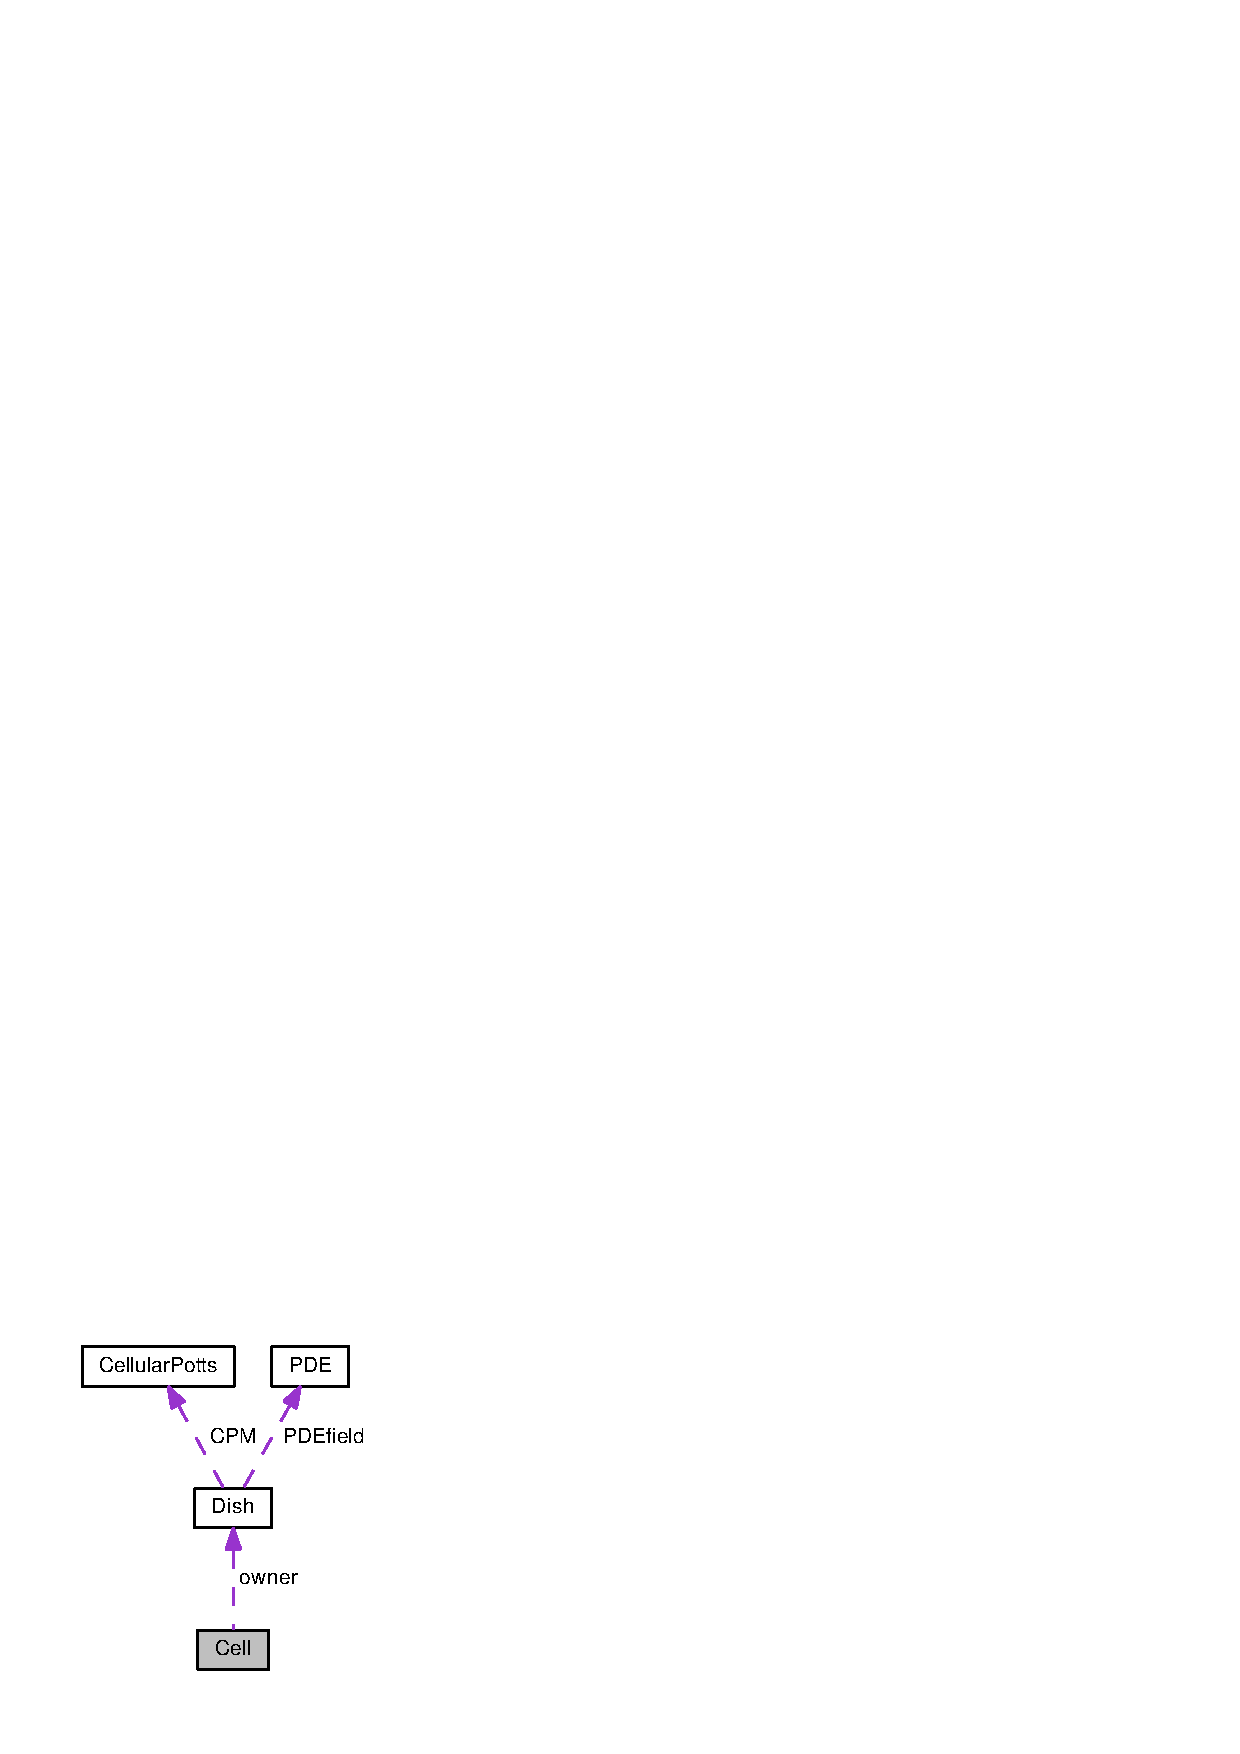
\includegraphics[width=179pt]{classCell__coll__graph}
\end{center}
\end{figure}
\subsection*{Public Member Functions}
\begin{DoxyCompactItemize}
\item 
{\bf Cell} (const {\bf Dish} \&who, int settau=1)
\begin{DoxyCompactList}\small\item\em Constructor to insert a cell into \doxyref{Dish}{p.}{classDish} \char`\"{}who\char`\"{}. \end{DoxyCompactList}\item 
{\bf Cell} (void)
\item 
{\bf $\sim$\-Cell} (void)
\item 
{\bf Cell} (const {\bf Cell} \&src)
\begin{DoxyCompactList}\small\item\em Default copy constructor. \end{DoxyCompactList}\item 
void {\bf Cell\-Birth} ({\bf Cell} \&{\bf mother})
\begin{DoxyCompactList}\small\item\em Add a new cell to the dish. \end{DoxyCompactList}\item 
{\bf Cell} \& {\bf operator=} (const {\bf Cell} \&src)
\begin{DoxyCompactList}\small\item\em Assignment operator. \end{DoxyCompactList}\item 
bool {\bf Alive\-P} (void) const 
\begin{DoxyCompactList}\small\item\em Returns false if \doxyref{Cell}{p.}{classCell} has apoptosed (vanished). \end{DoxyCompactList}\item 
int {\bf Colour} (void) const 
\begin{DoxyCompactList}\small\item\em Returns the cell colour. \end{DoxyCompactList}\item 
void {\bf set\-Tau} (int settau)
\begin{DoxyCompactList}\small\item\em Set cell type of this \doxyref{Cell}{p.}{classCell}. \end{DoxyCompactList}\item 
int {\bf get\-Tau} (void)
\begin{DoxyCompactList}\small\item\em Get cell type of this \doxyref{Cell}{p.}{classCell}. \end{DoxyCompactList}\item 
int {\bf Set\-Colour} (const int new\-\_\-colour)
\begin{DoxyCompactList}\small\item\em Set color of this cell to new\-\_\-colour, irrespective of type. \end{DoxyCompactList}\item 
int {\bf Energy\-Difference} (const {\bf Cell} \&cell2) const 
\item 
int {\bf Area} () const 
\begin{DoxyCompactList}\small\item\em Return \doxyref{Cell}{p.}{classCell}'s actual area. \end{DoxyCompactList}\item 
int {\bf Target\-Area} () const 
\begin{DoxyCompactList}\small\item\em Return \doxyref{Cell}{p.}{classCell}'s target area. \end{DoxyCompactList}\item 
double {\bf Target\-Length} () const 
\begin{DoxyCompactList}\small\item\em Return \doxyref{Cell}{p.}{classCell}'s target length. \end{DoxyCompactList}\item 
double {\bf Set\-Target\-Length} (double l)
\begin{DoxyCompactList}\small\item\em Set the \doxyref{Cell}{p.}{classCell}'s target length. \end{DoxyCompactList}\item 
void {\bf Print\-Inertia} (void)
\begin{DoxyCompactList}\small\item\em Debugging function used to print the cell's current inertia tensor (as used for calculations of the length ) \end{DoxyCompactList}\item 
double {\bf Length} (void)
\item 
void {\bf Renorm\-Polar\-Vec} (void)
\item 
int {\bf Sigma} () const 
\begin{DoxyCompactList}\small\item\em Returns the cell's cell identity number. \end{DoxyCompactList}\item 
int {\bf Set\-Target\-Area} (const int new\-\_\-area)
\begin{DoxyCompactList}\small\item\em Sets the target area of the cell. \end{DoxyCompactList}\item 
void {\bf Apoptose} ()
\begin{DoxyCompactList}\small\item\em Sends the current cell into apoptosis. \end{DoxyCompactList}\item 
int {\bf Increment\-Target\-Area} ()
\begin{DoxyCompactList}\small\item\em Decrement the cell's target area by one unit. \end{DoxyCompactList}\item 
int {\bf Decrement\-Target\-Area} ()
\begin{DoxyCompactList}\small\item\em Increment the cell's target area by one unit. \end{DoxyCompactList}\item 
int {\bf Mother} (void) const 
\begin{DoxyCompactList}\small\item\em \doxyref{Cell}{p.}{classCell} lineage tracking\-: get the cell's parent. \end{DoxyCompactList}\item 
int {\bf Daughter} (void) const 
\begin{DoxyCompactList}\small\item\em \doxyref{Cell}{p.}{classCell} lineage tracking\-: get the cell's daughter. \end{DoxyCompactList}\item 
int {\bf Times\-Divided} (void) const 
\begin{DoxyCompactList}\small\item\em Returns a counter keeping track of the number of divisions. \end{DoxyCompactList}\item 
int {\bf Date\-Of\-Birth} (void) const 
\begin{DoxyCompactList}\small\item\em Returns Monte Carlo Step (M\-C\-S) when this cell originated. \end{DoxyCompactList}\item 
int {\bf Colour\-Of\-Birth} (void) const 
\begin{DoxyCompactList}\small\item\em Returns the cell type at the time of birth. \end{DoxyCompactList}\item 
int {\bf Get\-J} (const {\bf Cell} \&c2) const 
\begin{DoxyCompactList}\small\item\em Returns the bond energy J between this cell and cell c2. \end{DoxyCompactList}\item 
double $\ast$ {\bf Set\-Grad} (double $\ast$g)
\begin{DoxyCompactList}\small\item\em Set the current gradient of the cell to g. Currently not in use. \end{DoxyCompactList}\item 
const double $\ast$ {\bf Get\-Grad} (void) const 
\begin{DoxyCompactList}\small\item\em Returns the cell's measured gradient. Currently not in use. \end{DoxyCompactList}\item 
const double {\bf Grad\-X} () const 
\begin{DoxyCompactList}\small\item\em Returns the cell's measured gradient. Currently not in use. \end{DoxyCompactList}\item 
const double {\bf Grad\-Y} () const 
\begin{DoxyCompactList}\small\item\em Returns the cell's measured gradient. Currently not in use. \end{DoxyCompactList}\item 
double $\ast$ {\bf Add\-To\-Grad} (double $\ast$g)
\begin{DoxyCompactList}\small\item\em Currently not in use (remove?) \end{DoxyCompactList}\item 
void {\bf Clear\-Grad} (void)
\begin{DoxyCompactList}\small\item\em Currently not in use (remove?) \end{DoxyCompactList}\item 
void {\bf Measure\-Cell\-Size} ({\bf Cell} \&c)
\end{DoxyCompactItemize}
\subsection*{Static Public Member Functions}
\begin{DoxyCompactItemize}
\item 
static void {\bf Clear\-J} (void)
\begin{DoxyCompactList}\small\item\em Clears the table of J's. \end{DoxyCompactList}\item 
static int {\bf Max\-Sigma} ()
\begin{DoxyCompactList}\small\item\em Returns the maximum cell identity number in the \doxyref{Dish}{p.}{classDish}. This would normally be the number of cells in the \doxyref{Dish}{p.}{classDish}, although the number includes apoptosed cells. \end{DoxyCompactList}\item 
static int {\bf Set\-J} (int t1, int t2, int val)
\begin{DoxyCompactList}\small\item\em Sets bond energy J between cell type t1 and t2 to val. \end{DoxyCompactList}\end{DoxyCompactItemize}
\subsection*{Public Attributes}
\begin{DoxyCompactItemize}
\item 
double {\bf polarvec} [9]
\end{DoxyCompactItemize}
\subsection*{Protected Attributes}
\begin{DoxyCompactItemize}
\item 
int {\bf colour}
\item 
bool {\bf alive}
\item 
int {\bf sigma}
\item 
int {\bf tau}
\item 
double {\bf length}
\item 
double {\bf target\-\_\-length}
\item 
int {\bf mother}
\item 
int {\bf daughter}
\item 
int {\bf times\-\_\-divided}
\item 
int {\bf date\-\_\-of\-\_\-birth}
\item 
int {\bf colour\-\_\-of\-\_\-birth}
\item 
int {\bf area}
\item 
int {\bf target\-\_\-area}
\item 
int {\bf growth\-\_\-threshold}
\item 
double {\bf v} [2]
\item 
int {\bf n\-\_\-copies}
\item 
double {\bf grad} [2]
\item 
double $\ast$ {\bf chem}
\item 
long int {\bf sum\-\_\-x}
\item 
long int {\bf sum\-\_\-y}
\item 
long int {\bf sum\-\_\-xx}
\item 
long int {\bf sum\-\_\-yy}
\item 
long int {\bf sum\-\_\-xy}
\item 
const {\bf Dish} $\ast$ {\bf owner}
\end{DoxyCompactItemize}
\subsection*{Static Protected Attributes}
\begin{DoxyCompactItemize}
\item 
static int $\ast$$\ast$ {\bf J} =0
\item 
static int {\bf maxtau} =0
\item 
static int {\bf amount} =0
\item 
static int {\bf capacity} =0
\item 
static int {\bf maxsigma} =0
\end{DoxyCompactItemize}
\subsection*{Friends}
\begin{DoxyCompactItemize}
\item 
class {\bf Dish}
\item 
class {\bf Cellular\-Potts}
\item 
class {\bf Info}
\end{DoxyCompactItemize}


\subsection{Constructor \& Destructor Documentation}
\index{Cell@{Cell}!Cell@{Cell}}
\index{Cell@{Cell}!Cell@{Cell}}
\subsubsection[{Cell}]{\setlength{\rightskip}{0pt plus 5cm}Cell\-::\-Cell (
\begin{DoxyParamCaption}
\item[{const {\bf Dish} \&}]{who, }
\item[{int}]{settau = {\ttfamily 1}}
\end{DoxyParamCaption}
)\hspace{0.3cm}{\ttfamily [inline]}}\label{classCell_a822aecd83d8aa95fab97641a88e60225}


Constructor to insert a cell into \doxyref{Dish}{p.}{classDish} \char`\"{}who\char`\"{}. 

Used to add a new \doxyref{Cell}{p.}{classCell} to the dish\-: new \doxyref{Cell}{p.}{classCell}(dish, celtype). 

References owner.

\index{Cell@{Cell}!Cell@{Cell}}
\index{Cell@{Cell}!Cell@{Cell}}
\subsubsection[{Cell}]{\setlength{\rightskip}{0pt plus 5cm}Cell\-::\-Cell (
\begin{DoxyParamCaption}
\item[{void}]{}
\end{DoxyParamCaption}
)\hspace{0.3cm}{\ttfamily [inline]}}\label{classCell_aab24f3f223f86c03968096edbd40a9f0}


References chem, and Parameter\-::n\-\_\-chem.

\index{Cell@{Cell}!$\sim$\-Cell@{$\sim$\-Cell}}
\index{$\sim$\-Cell@{$\sim$\-Cell}!Cell@{Cell}}
\subsubsection[{$\sim$\-Cell}]{\setlength{\rightskip}{0pt plus 5cm}Cell\-::$\sim$\-Cell (
\begin{DoxyParamCaption}
\item[{void}]{}
\end{DoxyParamCaption}
)}\label{classCell_a4206c923493126fb2f01c8cf53c78e69}
\index{Cell@{Cell}!Cell@{Cell}}
\index{Cell@{Cell}!Cell@{Cell}}
\subsubsection[{Cell}]{\setlength{\rightskip}{0pt plus 5cm}Cell\-::\-Cell (
\begin{DoxyParamCaption}
\item[{const {\bf Cell} \&}]{src}
\end{DoxyParamCaption}
)\hspace{0.3cm}{\ttfamily [inline]}}\label{classCell_a8a36eee6405552ddb5a27d2ce1a7272c}


Default copy constructor. 



References alive, amount, area, chem, colour\-\_\-of\-\_\-birth, date\-\_\-of\-\_\-birth, daughter, growth\-\_\-threshold, length, mother, Parameter\-::n\-\_\-chem, n\-\_\-copies, owner, sigma, sum\-\_\-x, sum\-\_\-xx, sum\-\_\-xy, sum\-\_\-y, sum\-\_\-yy, target\-\_\-area, target\-\_\-length, tau, times\-\_\-divided, and v.



\subsection{Member Function Documentation}
\index{Cell@{Cell}!Add\-To\-Grad@{Add\-To\-Grad}}
\index{Add\-To\-Grad@{Add\-To\-Grad}!Cell@{Cell}}
\subsubsection[{Add\-To\-Grad}]{\setlength{\rightskip}{0pt plus 5cm}double$\ast$ Cell\-::\-Add\-To\-Grad (
\begin{DoxyParamCaption}
\item[{double $\ast$}]{g}
\end{DoxyParamCaption}
)\hspace{0.3cm}{\ttfamily [inline]}}\label{classCell_a1f752d55345bfd01eed50f3f31759678}


Currently not in use (remove?) 



References grad.

\index{Cell@{Cell}!Alive\-P@{Alive\-P}}
\index{Alive\-P@{Alive\-P}!Cell@{Cell}}
\subsubsection[{Alive\-P}]{\setlength{\rightskip}{0pt plus 5cm}bool Cell\-::\-Alive\-P (
\begin{DoxyParamCaption}
\item[{void}]{}
\end{DoxyParamCaption}
) const\hspace{0.3cm}{\ttfamily [inline]}}\label{classCell_afcd8b017af857ae54f43c914d42ecef8}


Returns false if \doxyref{Cell}{p.}{classCell} has apoptosed (vanished). 



References alive.

\index{Cell@{Cell}!Apoptose@{Apoptose}}
\index{Apoptose@{Apoptose}!Cell@{Cell}}
\subsubsection[{Apoptose}]{\setlength{\rightskip}{0pt plus 5cm}void Cell\-::\-Apoptose (
\begin{DoxyParamCaption}
{}
\end{DoxyParamCaption}
)\hspace{0.3cm}{\ttfamily [inline]}}\label{classCell_a2b598309713229d89b14d7c1aa7d151a}


Sends the current cell into apoptosis. 



References alive.

\index{Cell@{Cell}!Area@{Area}}
\index{Area@{Area}!Cell@{Cell}}
\subsubsection[{Area}]{\setlength{\rightskip}{0pt plus 5cm}int Cell\-::\-Area (
\begin{DoxyParamCaption}
{}
\end{DoxyParamCaption}
) const\hspace{0.3cm}{\ttfamily [inline]}}\label{classCell_a21aa74dfaf504ffb34d9ab3a85a02e81}


Return \doxyref{Cell}{p.}{classCell}'s actual area. 



References area.



Referenced by Cellular\-Potts\-::\-Compactness(), Cellular\-Potts\-::\-Mean\-Cell\-Area(), Dish\-::\-Measure\-Chem\-Concentrations(), and Info\-::\-Menu().

\index{Cell@{Cell}!Cell\-Birth@{Cell\-Birth}}
\index{Cell\-Birth@{Cell\-Birth}!Cell@{Cell}}
\subsubsection[{Cell\-Birth}]{\setlength{\rightskip}{0pt plus 5cm}void Cell\-::\-Cell\-Birth (
\begin{DoxyParamCaption}
\item[{{\bf Cell} \&}]{mother}
\end{DoxyParamCaption}
)}\label{classCell_a387af5e97fced410b231aa730d87dd33}


Add a new cell to the dish. 

Call it as\-: new \doxyref{Cell(parent, true)}{p.}{classCell}; mother will be modified for ancestry administration!


\begin{DoxyParams}{Parameters}
{\em settau} & \doxyref{Cell}{p.}{classCell} type of daughter cell. \\
\hline
\end{DoxyParams}


References alive, chem, colour, daughter, grad, Parameter\-::n\-\_\-chem, owner, sigma, target\-\_\-length, tau, Dish\-::\-Time(), times\-\_\-divided, and v.

\index{Cell@{Cell}!Clear\-Grad@{Clear\-Grad}}
\index{Clear\-Grad@{Clear\-Grad}!Cell@{Cell}}
\subsubsection[{Clear\-Grad}]{\setlength{\rightskip}{0pt plus 5cm}void Cell\-::\-Clear\-Grad (
\begin{DoxyParamCaption}
\item[{void}]{}
\end{DoxyParamCaption}
)\hspace{0.3cm}{\ttfamily [inline]}}\label{classCell_a9c3fd8e71b9272d5229e3fad2761c321}


Currently not in use (remove?) 



References grad.

\index{Cell@{Cell}!Clear\-J@{Clear\-J}}
\index{Clear\-J@{Clear\-J}!Cell@{Cell}}
\subsubsection[{Clear\-J}]{\setlength{\rightskip}{0pt plus 5cm}void Cell\-::\-Clear\-J (
\begin{DoxyParamCaption}
\item[{void}]{}
\end{DoxyParamCaption}
)\hspace{0.3cm}{\ttfamily [static]}}\label{classCell_a8baa793d28c592ee85d63ad52ac2fb7d}


Clears the table of J's. 

This is only important for a feature called \char`\"{}\-Dynamic\-J's\char`\"{}, where J-\/values depend on internal states of the cells (such as a genetic network; see e.\-g. Hogeweg et al. 2000). The current version of T\-S\-T does not include such functionality. 

References E\-M\-P\-T\-Y.

\index{Cell@{Cell}!Colour@{Colour}}
\index{Colour@{Colour}!Cell@{Cell}}
\subsubsection[{Colour}]{\setlength{\rightskip}{0pt plus 5cm}int Cell\-::\-Colour (
\begin{DoxyParamCaption}
\item[{void}]{}
\end{DoxyParamCaption}
) const\hspace{0.3cm}{\ttfamily [inline]}}\label{classCell_a90cb6d57ff7baac384ea61fe2874747b}


Returns the cell colour. 



References tau.



Referenced by Info\-::\-Menu().

\index{Cell@{Cell}!Colour\-Of\-Birth@{Colour\-Of\-Birth}}
\index{Colour\-Of\-Birth@{Colour\-Of\-Birth}!Cell@{Cell}}
\subsubsection[{Colour\-Of\-Birth}]{\setlength{\rightskip}{0pt plus 5cm}int Cell\-::\-Colour\-Of\-Birth (
\begin{DoxyParamCaption}
\item[{void}]{}
\end{DoxyParamCaption}
) const\hspace{0.3cm}{\ttfamily [inline]}}\label{classCell_ae7905782540a639ddb1565e688106274}


Returns the cell type at the time of birth. 



References colour\-\_\-of\-\_\-birth.

\index{Cell@{Cell}!Date\-Of\-Birth@{Date\-Of\-Birth}}
\index{Date\-Of\-Birth@{Date\-Of\-Birth}!Cell@{Cell}}
\subsubsection[{Date\-Of\-Birth}]{\setlength{\rightskip}{0pt plus 5cm}int Cell\-::\-Date\-Of\-Birth (
\begin{DoxyParamCaption}
\item[{void}]{}
\end{DoxyParamCaption}
) const\hspace{0.3cm}{\ttfamily [inline]}}\label{classCell_a315f8306c20cd71e1199c5c27b6d7cd6}


Returns Monte Carlo Step (M\-C\-S) when this cell originated. 



References date\-\_\-of\-\_\-birth.

\index{Cell@{Cell}!Daughter@{Daughter}}
\index{Daughter@{Daughter}!Cell@{Cell}}
\subsubsection[{Daughter}]{\setlength{\rightskip}{0pt plus 5cm}int Cell\-::\-Daughter (
\begin{DoxyParamCaption}
\item[{void}]{}
\end{DoxyParamCaption}
) const\hspace{0.3cm}{\ttfamily [inline]}}\label{classCell_afc0c6d621b71384ff00ece060eb2b8b5}


\doxyref{Cell}{p.}{classCell} lineage tracking\-: get the cell's daughter. 



References daughter.

\index{Cell@{Cell}!Decrement\-Target\-Area@{Decrement\-Target\-Area}}
\index{Decrement\-Target\-Area@{Decrement\-Target\-Area}!Cell@{Cell}}
\subsubsection[{Decrement\-Target\-Area}]{\setlength{\rightskip}{0pt plus 5cm}int Cell\-::\-Decrement\-Target\-Area (
\begin{DoxyParamCaption}
{}
\end{DoxyParamCaption}
)\hspace{0.3cm}{\ttfamily [inline]}}\label{classCell_a9b90cf417c4fb1df8b4b005e6858a754}


Increment the cell's target area by one unit. 



References target\-\_\-area.

\index{Cell@{Cell}!Energy\-Difference@{Energy\-Difference}}
\index{Energy\-Difference@{Energy\-Difference}!Cell@{Cell}}
\subsubsection[{Energy\-Difference}]{\setlength{\rightskip}{0pt plus 5cm}int Cell\-::\-Energy\-Difference (
\begin{DoxyParamCaption}
\item[{const {\bf Cell} \&}]{cell2}
\end{DoxyParamCaption}
) const}\label{classCell_a2e48645e8b7e78f2f6718fe59e171717}


References sigma, and tau.

\index{Cell@{Cell}!Get\-Grad@{Get\-Grad}}
\index{Get\-Grad@{Get\-Grad}!Cell@{Cell}}
\subsubsection[{Get\-Grad}]{\setlength{\rightskip}{0pt plus 5cm}const double$\ast$ Cell\-::\-Get\-Grad (
\begin{DoxyParamCaption}
\item[{void}]{}
\end{DoxyParamCaption}
) const\hspace{0.3cm}{\ttfamily [inline]}}\label{classCell_a33637f75f6f371eff9e9ddeb21e122e7}


Returns the cell's measured gradient. Currently not in use. 



References grad.

\index{Cell@{Cell}!Get\-J@{Get\-J}}
\index{Get\-J@{Get\-J}!Cell@{Cell}}
\subsubsection[{Get\-J}]{\setlength{\rightskip}{0pt plus 5cm}int Cell\-::\-Get\-J (
\begin{DoxyParamCaption}
\item[{const {\bf Cell} \&}]{c2}
\end{DoxyParamCaption}
) const\hspace{0.3cm}{\ttfamily [inline]}}\label{classCell_a1e3148b7392cc2b4bb8a1887d26536e1}


Returns the bond energy J between this cell and cell c2. 



References J, and sigma.

\index{Cell@{Cell}!get\-Tau@{get\-Tau}}
\index{get\-Tau@{get\-Tau}!Cell@{Cell}}
\subsubsection[{get\-Tau}]{\setlength{\rightskip}{0pt plus 5cm}int Cell\-::get\-Tau (
\begin{DoxyParamCaption}
\item[{void}]{}
\end{DoxyParamCaption}
)\hspace{0.3cm}{\ttfamily [inline]}}\label{classCell_a9fbfdfe12c82591083e673987d35570a}


Get cell type of this \doxyref{Cell}{p.}{classCell}. 



References tau.

\index{Cell@{Cell}!Grad\-X@{Grad\-X}}
\index{Grad\-X@{Grad\-X}!Cell@{Cell}}
\subsubsection[{Grad\-X}]{\setlength{\rightskip}{0pt plus 5cm}const double Cell\-::\-Grad\-X (
\begin{DoxyParamCaption}
{}
\end{DoxyParamCaption}
) const\hspace{0.3cm}{\ttfamily [inline]}}\label{classCell_a173e84b97374593b5296a4a61b7c520b}


Returns the cell's measured gradient. Currently not in use. 



References grad.

\index{Cell@{Cell}!Grad\-Y@{Grad\-Y}}
\index{Grad\-Y@{Grad\-Y}!Cell@{Cell}}
\subsubsection[{Grad\-Y}]{\setlength{\rightskip}{0pt plus 5cm}const double Cell\-::\-Grad\-Y (
\begin{DoxyParamCaption}
{}
\end{DoxyParamCaption}
) const\hspace{0.3cm}{\ttfamily [inline]}}\label{classCell_a6119f2bdff326bd7bbcdbcb8495f3c22}


Returns the cell's measured gradient. Currently not in use. 



References grad.

\index{Cell@{Cell}!Increment\-Target\-Area@{Increment\-Target\-Area}}
\index{Increment\-Target\-Area@{Increment\-Target\-Area}!Cell@{Cell}}
\subsubsection[{Increment\-Target\-Area}]{\setlength{\rightskip}{0pt plus 5cm}int Cell\-::\-Increment\-Target\-Area (
\begin{DoxyParamCaption}
{}
\end{DoxyParamCaption}
)\hspace{0.3cm}{\ttfamily [inline]}}\label{classCell_a89086e3c8e2c7619030f86b0fcd2a0b2}


Decrement the cell's target area by one unit. 



References target\-\_\-area.



Referenced by Dish\-::\-Cell\-Growth\-And\-Division().

\index{Cell@{Cell}!Length@{Length}}
\index{Length@{Length}!Cell@{Cell}}
\subsubsection[{Length}]{\setlength{\rightskip}{0pt plus 5cm}double Cell\-::\-Length (
\begin{DoxyParamCaption}
\item[{void}]{}
\end{DoxyParamCaption}
)\hspace{0.3cm}{\ttfamily [inline]}}\label{classCell_ac038876b1cc38b8efea7338c853b98ca}


References length.

\index{Cell@{Cell}!Max\-Sigma@{Max\-Sigma}}
\index{Max\-Sigma@{Max\-Sigma}!Cell@{Cell}}
\subsubsection[{Max\-Sigma}]{\setlength{\rightskip}{0pt plus 5cm}static int Cell\-::\-Max\-Sigma (
\begin{DoxyParamCaption}
{}
\end{DoxyParamCaption}
)\hspace{0.3cm}{\ttfamily [inline]}, {\ttfamily [static]}}\label{classCell_a8b1e24a10e09376d69e7e52a39c5fad1}


Returns the maximum cell identity number in the \doxyref{Dish}{p.}{classDish}. This would normally be the number of cells in the \doxyref{Dish}{p.}{classDish}, although the number includes apoptosed cells. 



References maxsigma.



Referenced by Cellular\-Potts\-::\-Read\-Zygote\-Picture().

\index{Cell@{Cell}!Measure\-Cell\-Size@{Measure\-Cell\-Size}}
\index{Measure\-Cell\-Size@{Measure\-Cell\-Size}!Cell@{Cell}}
\subsubsection[{Measure\-Cell\-Size}]{\setlength{\rightskip}{0pt plus 5cm}void Cell\-::\-Measure\-Cell\-Size (
\begin{DoxyParamCaption}
\item[{{\bf Cell} \&}]{c}
\end{DoxyParamCaption}
)}\label{classCell_a8e798cf1b3cacb03713a9e45bca961e1}
After introducing a new \doxyref{Cell}{p.}{classCell} (e.\-g. with Grow\-In\-Cell) call this function to set the moments and areas right. 

Referenced by Info\-::\-Menu().

\index{Cell@{Cell}!Mother@{Mother}}
\index{Mother@{Mother}!Cell@{Cell}}
\subsubsection[{Mother}]{\setlength{\rightskip}{0pt plus 5cm}int Cell\-::\-Mother (
\begin{DoxyParamCaption}
\item[{void}]{}
\end{DoxyParamCaption}
) const\hspace{0.3cm}{\ttfamily [inline]}}\label{classCell_a1b0f0d4b8d528f76b55bccb1ecdabb2f}


\doxyref{Cell}{p.}{classCell} lineage tracking\-: get the cell's parent. 



References mother.

\index{Cell@{Cell}!operator=@{operator=}}
\index{operator=@{operator=}!Cell@{Cell}}
\subsubsection[{operator=}]{\setlength{\rightskip}{0pt plus 5cm}{\bf Cell}\& Cell\-::operator= (
\begin{DoxyParamCaption}
\item[{const {\bf Cell} \&}]{src}
\end{DoxyParamCaption}
)\hspace{0.3cm}{\ttfamily [inline]}}\label{classCell_a1cd1d7177642c146770197ef0eb3b55c}


Assignment operator. 

Called if one cell is assigned to another. Remember to change both assignment operator and copy constructor when adding new attributes to \doxyref{Cell}{p.}{classCell}. 

References alive, amount, area, chem, colour, length, Parameter\-::n\-\_\-chem, n\-\_\-copies, owner, sigma, sum\-\_\-x, sum\-\_\-xx, sum\-\_\-xy, sum\-\_\-y, sum\-\_\-yy, target\-\_\-area, target\-\_\-length, tau, and v.

\index{Cell@{Cell}!Print\-Inertia@{Print\-Inertia}}
\index{Print\-Inertia@{Print\-Inertia}!Cell@{Cell}}
\subsubsection[{Print\-Inertia}]{\setlength{\rightskip}{0pt plus 5cm}void Cell\-::\-Print\-Inertia (
\begin{DoxyParamCaption}
\item[{void}]{}
\end{DoxyParamCaption}
)\hspace{0.3cm}{\ttfamily [inline]}}\label{classCell_a4cdc14c24736d472c100a3382c3577c8}


Debugging function used to print the cell's current inertia tensor (as used for calculations of the length ) 



References area, sum\-\_\-x, sum\-\_\-xx, sum\-\_\-xy, sum\-\_\-y, and sum\-\_\-yy.

\index{Cell@{Cell}!Renorm\-Polar\-Vec@{Renorm\-Polar\-Vec}}
\index{Renorm\-Polar\-Vec@{Renorm\-Polar\-Vec}!Cell@{Cell}}
\subsubsection[{Renorm\-Polar\-Vec}]{\setlength{\rightskip}{0pt plus 5cm}void Cell\-::\-Renorm\-Polar\-Vec (
\begin{DoxyParamCaption}
\item[{void}]{}
\end{DoxyParamCaption}
)}\label{classCell_aa7117746e515e58cddc97362a9e244b0}
\index{Cell@{Cell}!Set\-Colour@{Set\-Colour}}
\index{Set\-Colour@{Set\-Colour}!Cell@{Cell}}
\subsubsection[{Set\-Colour}]{\setlength{\rightskip}{0pt plus 5cm}int Cell\-::\-Set\-Colour (
\begin{DoxyParamCaption}
\item[{const int}]{new\-\_\-colour}
\end{DoxyParamCaption}
)\hspace{0.3cm}{\ttfamily [inline]}}\label{classCell_aeafe2f67bdc876223f8871eb9f3e16ef}


Set color of this cell to new\-\_\-colour, irrespective of type. 



References colour.

\index{Cell@{Cell}!Set\-Grad@{Set\-Grad}}
\index{Set\-Grad@{Set\-Grad}!Cell@{Cell}}
\subsubsection[{Set\-Grad}]{\setlength{\rightskip}{0pt plus 5cm}double$\ast$ Cell\-::\-Set\-Grad (
\begin{DoxyParamCaption}
\item[{double $\ast$}]{g}
\end{DoxyParamCaption}
)\hspace{0.3cm}{\ttfamily [inline]}}\label{classCell_a45ba19b4e704592fd0cdd5270912fce2}


Set the current gradient of the cell to g. Currently not in use. 



References grad.

\index{Cell@{Cell}!Set\-J@{Set\-J}}
\index{Set\-J@{Set\-J}!Cell@{Cell}}
\subsubsection[{Set\-J}]{\setlength{\rightskip}{0pt plus 5cm}static int Cell\-::\-Set\-J (
\begin{DoxyParamCaption}
\item[{int}]{t1, }
\item[{int}]{t2, }
\item[{int}]{val}
\end{DoxyParamCaption}
)\hspace{0.3cm}{\ttfamily [inline]}, {\ttfamily [static]}}\label{classCell_a98f324f5c5829e53188c589373dc9f98}


Sets bond energy J between cell type t1 and t2 to val. 



References J.

\index{Cell@{Cell}!Set\-Target\-Area@{Set\-Target\-Area}}
\index{Set\-Target\-Area@{Set\-Target\-Area}!Cell@{Cell}}
\subsubsection[{Set\-Target\-Area}]{\setlength{\rightskip}{0pt plus 5cm}int Cell\-::\-Set\-Target\-Area (
\begin{DoxyParamCaption}
\item[{const int}]{new\-\_\-area}
\end{DoxyParamCaption}
)\hspace{0.3cm}{\ttfamily [inline]}}\label{classCell_a0f78f87720f0eca3520678bea6194b9f}


Sets the target area of the cell. 



References target\-\_\-area.



Referenced by Cellular\-Potts\-::\-Grow\-And\-Divide\-Cells(), and Info\-::\-Menu().

\index{Cell@{Cell}!Set\-Target\-Length@{Set\-Target\-Length}}
\index{Set\-Target\-Length@{Set\-Target\-Length}!Cell@{Cell}}
\subsubsection[{Set\-Target\-Length}]{\setlength{\rightskip}{0pt plus 5cm}double Cell\-::\-Set\-Target\-Length (
\begin{DoxyParamCaption}
\item[{double}]{l}
\end{DoxyParamCaption}
)\hspace{0.3cm}{\ttfamily [inline]}}\label{classCell_af4cacfabcefaec22f4c875bf7566f67d}


Set the \doxyref{Cell}{p.}{classCell}'s target length. 



References target\-\_\-length.



Referenced by Info\-::\-Menu(), and Cellular\-Potts\-::\-Reset\-Target\-Lengths().

\index{Cell@{Cell}!set\-Tau@{set\-Tau}}
\index{set\-Tau@{set\-Tau}!Cell@{Cell}}
\subsubsection[{set\-Tau}]{\setlength{\rightskip}{0pt plus 5cm}void Cell\-::set\-Tau (
\begin{DoxyParamCaption}
\item[{int}]{settau}
\end{DoxyParamCaption}
)\hspace{0.3cm}{\ttfamily [inline]}}\label{classCell_af3a3882fdf4e48130af67184cc70fe9d}


Set cell type of this \doxyref{Cell}{p.}{classCell}. 



References tau.



Referenced by Info\-::\-Menu().

\index{Cell@{Cell}!Sigma@{Sigma}}
\index{Sigma@{Sigma}!Cell@{Cell}}
\subsubsection[{Sigma}]{\setlength{\rightskip}{0pt plus 5cm}int Cell\-::\-Sigma (
\begin{DoxyParamCaption}
{}
\end{DoxyParamCaption}
) const\hspace{0.3cm}{\ttfamily [inline]}}\label{classCell_a348e0b2e02d03aa5f1cd4ab3ca8d16f0}


Returns the cell's cell identity number. 



References sigma.



Referenced by Info\-::\-Menu().

\index{Cell@{Cell}!Target\-Area@{Target\-Area}}
\index{Target\-Area@{Target\-Area}!Cell@{Cell}}
\subsubsection[{Target\-Area}]{\setlength{\rightskip}{0pt plus 5cm}int Cell\-::\-Target\-Area (
\begin{DoxyParamCaption}
{}
\end{DoxyParamCaption}
) const\hspace{0.3cm}{\ttfamily [inline]}}\label{classCell_a50535c6a42e2a462a44025129a72f93b}


Return \doxyref{Cell}{p.}{classCell}'s target area. 



References target\-\_\-area.



Referenced by Info\-::\-Menu().

\index{Cell@{Cell}!Target\-Length@{Target\-Length}}
\index{Target\-Length@{Target\-Length}!Cell@{Cell}}
\subsubsection[{Target\-Length}]{\setlength{\rightskip}{0pt plus 5cm}double Cell\-::\-Target\-Length (
\begin{DoxyParamCaption}
{}
\end{DoxyParamCaption}
) const\hspace{0.3cm}{\ttfamily [inline]}}\label{classCell_aac717d05dbf104463bcf51b9a8480843}


Return \doxyref{Cell}{p.}{classCell}'s target length. 

Length constraint is documented in Merks et al. 2006, Dev. Biol. 

References target\-\_\-length.

\index{Cell@{Cell}!Times\-Divided@{Times\-Divided}}
\index{Times\-Divided@{Times\-Divided}!Cell@{Cell}}
\subsubsection[{Times\-Divided}]{\setlength{\rightskip}{0pt plus 5cm}int Cell\-::\-Times\-Divided (
\begin{DoxyParamCaption}
\item[{void}]{}
\end{DoxyParamCaption}
) const\hspace{0.3cm}{\ttfamily [inline]}}\label{classCell_a5ff760f8ace1a7d47813441dcce6f2fe}


Returns a counter keeping track of the number of divisions. 



References times\-\_\-divided.



\subsection{Friends And Related Function Documentation}
\index{Cell@{Cell}!Cellular\-Potts@{Cellular\-Potts}}
\index{Cellular\-Potts@{Cellular\-Potts}!Cell@{Cell}}
\subsubsection[{Cellular\-Potts}]{\setlength{\rightskip}{0pt plus 5cm}friend class {\bf Cellular\-Potts}\hspace{0.3cm}{\ttfamily [friend]}}\label{classCell_ac0d1ad5d66ebb242178dd5da9c9d6fca}
\index{Cell@{Cell}!Dish@{Dish}}
\index{Dish@{Dish}!Cell@{Cell}}
\subsubsection[{Dish}]{\setlength{\rightskip}{0pt plus 5cm}friend class {\bf Dish}\hspace{0.3cm}{\ttfamily [friend]}}\label{classCell_aed9cb4dbc4f47dbc026e3287f7c2831b}
\index{Cell@{Cell}!Info@{Info}}
\index{Info@{Info}!Cell@{Cell}}
\subsubsection[{Info}]{\setlength{\rightskip}{0pt plus 5cm}friend class {\bf Info}\hspace{0.3cm}{\ttfamily [friend]}}\label{classCell_a4838ff865b8d8625c61d208a420f8212}


\subsection{Member Data Documentation}
\index{Cell@{Cell}!alive@{alive}}
\index{alive@{alive}!Cell@{Cell}}
\subsubsection[{alive}]{\setlength{\rightskip}{0pt plus 5cm}bool Cell\-::alive\hspace{0.3cm}{\ttfamily [protected]}}\label{classCell_a516ed0ccc2782e870bfe6ba56d15d86b}


Referenced by Alive\-P(), Apoptose(), Cell(), Cell\-Birth(), and operator=().

\index{Cell@{Cell}!amount@{amount}}
\index{amount@{amount}!Cell@{Cell}}
\subsubsection[{amount}]{\setlength{\rightskip}{0pt plus 5cm}int Cell\-::amount =0\hspace{0.3cm}{\ttfamily [static]}, {\ttfamily [protected]}}\label{classCell_a92a252a4aec7850e2bea34fcfd6ec5f0}


Referenced by Cell(), and operator=().

\index{Cell@{Cell}!area@{area}}
\index{area@{area}!Cell@{Cell}}
\subsubsection[{area}]{\setlength{\rightskip}{0pt plus 5cm}int Cell\-::area\hspace{0.3cm}{\ttfamily [protected]}}\label{classCell_ab8c82c118a975064f24933950c225133}


Referenced by Area(), Cell(), operator=(), and Print\-Inertia().

\index{Cell@{Cell}!capacity@{capacity}}
\index{capacity@{capacity}!Cell@{Cell}}
\subsubsection[{capacity}]{\setlength{\rightskip}{0pt plus 5cm}int Cell\-::capacity =0\hspace{0.3cm}{\ttfamily [static]}, {\ttfamily [protected]}}\label{classCell_a13afbf7c2a81d591cc414e8cc6965ad4}
\index{Cell@{Cell}!chem@{chem}}
\index{chem@{chem}!Cell@{Cell}}
\subsubsection[{chem}]{\setlength{\rightskip}{0pt plus 5cm}double$\ast$ Cell\-::chem\hspace{0.3cm}{\ttfamily [protected]}}\label{classCell_a67e85d8f9025fc82f44ce7e266021133}


Referenced by Cell(), Cell\-Birth(), Dish\-::\-Measure\-Chem\-Concentrations(), and operator=().

\index{Cell@{Cell}!colour@{colour}}
\index{colour@{colour}!Cell@{Cell}}
\subsubsection[{colour}]{\setlength{\rightskip}{0pt plus 5cm}int Cell\-::colour\hspace{0.3cm}{\ttfamily [protected]}}\label{classCell_a3a62f75d92e0a0225554c963e543f428}


Referenced by Cell\-Birth(), operator=(), and Set\-Colour().

\index{Cell@{Cell}!colour\-\_\-of\-\_\-birth@{colour\-\_\-of\-\_\-birth}}
\index{colour\-\_\-of\-\_\-birth@{colour\-\_\-of\-\_\-birth}!Cell@{Cell}}
\subsubsection[{colour\-\_\-of\-\_\-birth}]{\setlength{\rightskip}{0pt plus 5cm}int Cell\-::colour\-\_\-of\-\_\-birth\hspace{0.3cm}{\ttfamily [protected]}}\label{classCell_a7e116fda8ff80b6ebb03b9c43584a68c}


Referenced by Cell(), and Colour\-Of\-Birth().

\index{Cell@{Cell}!date\-\_\-of\-\_\-birth@{date\-\_\-of\-\_\-birth}}
\index{date\-\_\-of\-\_\-birth@{date\-\_\-of\-\_\-birth}!Cell@{Cell}}
\subsubsection[{date\-\_\-of\-\_\-birth}]{\setlength{\rightskip}{0pt plus 5cm}int Cell\-::date\-\_\-of\-\_\-birth\hspace{0.3cm}{\ttfamily [protected]}}\label{classCell_a9c97f4e44e305b2f39e953ba607e729a}


Referenced by Cell(), and Date\-Of\-Birth().

\index{Cell@{Cell}!daughter@{daughter}}
\index{daughter@{daughter}!Cell@{Cell}}
\subsubsection[{daughter}]{\setlength{\rightskip}{0pt plus 5cm}int Cell\-::daughter\hspace{0.3cm}{\ttfamily [protected]}}\label{classCell_a90a992f97f2316d043904caaffd7e439}


Referenced by Cell(), Cell\-Birth(), and Daughter().

\index{Cell@{Cell}!grad@{grad}}
\index{grad@{grad}!Cell@{Cell}}
\subsubsection[{grad}]{\setlength{\rightskip}{0pt plus 5cm}double Cell\-::grad[2]\hspace{0.3cm}{\ttfamily [protected]}}\label{classCell_aba7f037648153483d44f04d3cea7ef37}


Referenced by Add\-To\-Grad(), Cell\-Birth(), Clear\-Grad(), Get\-Grad(), Grad\-X(), Grad\-Y(), and Set\-Grad().

\index{Cell@{Cell}!growth\-\_\-threshold@{growth\-\_\-threshold}}
\index{growth\-\_\-threshold@{growth\-\_\-threshold}!Cell@{Cell}}
\subsubsection[{growth\-\_\-threshold}]{\setlength{\rightskip}{0pt plus 5cm}int Cell\-::growth\-\_\-threshold\hspace{0.3cm}{\ttfamily [protected]}}\label{classCell_ac0ec22ca2c2b77be00ade91ec2c176e2}


Referenced by Cell().

\index{Cell@{Cell}!J@{J}}
\index{J@{J}!Cell@{Cell}}
\subsubsection[{J}]{\setlength{\rightskip}{0pt plus 5cm}int $\ast$$\ast$ Cell\-::\-J =0\hspace{0.3cm}{\ttfamily [static]}, {\ttfamily [protected]}}\label{classCell_a7c7fb58882da8d7185438d4dcf44b291}


Referenced by Get\-J(), and Set\-J().

\index{Cell@{Cell}!length@{length}}
\index{length@{length}!Cell@{Cell}}
\subsubsection[{length}]{\setlength{\rightskip}{0pt plus 5cm}double Cell\-::length\hspace{0.3cm}{\ttfamily [protected]}}\label{classCell_a10a70197c4e757ad39177b146b5c2a67}


Referenced by Cell(), Length(), and operator=().

\index{Cell@{Cell}!maxsigma@{maxsigma}}
\index{maxsigma@{maxsigma}!Cell@{Cell}}
\subsubsection[{maxsigma}]{\setlength{\rightskip}{0pt plus 5cm}int Cell\-::maxsigma =0\hspace{0.3cm}{\ttfamily [static]}, {\ttfamily [protected]}}\label{classCell_ab423587adbfdc733ae4311c7e1ed3065}


Referenced by Dish\-::\-Constructor\-Body(), and Max\-Sigma().

\index{Cell@{Cell}!maxtau@{maxtau}}
\index{maxtau@{maxtau}!Cell@{Cell}}
\subsubsection[{maxtau}]{\setlength{\rightskip}{0pt plus 5cm}int Cell\-::maxtau =0\hspace{0.3cm}{\ttfamily [static]}, {\ttfamily [protected]}}\label{classCell_aca2b6fa3035757ea4c2cd8f30f7610ae}


Referenced by Cellular\-Potts\-::\-Set\-Random\-Types().

\index{Cell@{Cell}!mother@{mother}}
\index{mother@{mother}!Cell@{Cell}}
\subsubsection[{mother}]{\setlength{\rightskip}{0pt plus 5cm}int Cell\-::mother\hspace{0.3cm}{\ttfamily [protected]}}\label{classCell_a74435ead6958823c8c2f3e8f55d4429a}


Referenced by Cell(), and Mother().

\index{Cell@{Cell}!n\-\_\-copies@{n\-\_\-copies}}
\index{n\-\_\-copies@{n\-\_\-copies}!Cell@{Cell}}
\subsubsection[{n\-\_\-copies}]{\setlength{\rightskip}{0pt plus 5cm}int Cell\-::n\-\_\-copies\hspace{0.3cm}{\ttfamily [protected]}}\label{classCell_ac374476768b00e014877a8ff9097ebb8}


Referenced by Cell(), and operator=().

\index{Cell@{Cell}!owner@{owner}}
\index{owner@{owner}!Cell@{Cell}}
\subsubsection[{owner}]{\setlength{\rightskip}{0pt plus 5cm}const {\bf Dish}$\ast$ Cell\-::owner\hspace{0.3cm}{\ttfamily [protected]}}\label{classCell_a5ba3270256dca27969f1888cd9eb7a35}


Referenced by Cell(), Cell\-Birth(), operator=(), and Dish\-::\-Set\-Cell\-Owner().

\index{Cell@{Cell}!polarvec@{polarvec}}
\index{polarvec@{polarvec}!Cell@{Cell}}
\subsubsection[{polarvec}]{\setlength{\rightskip}{0pt plus 5cm}double Cell\-::polarvec[9]}\label{classCell_ad740a0c567d6adc4f5a4446f6066aefa}
\index{Cell@{Cell}!sigma@{sigma}}
\index{sigma@{sigma}!Cell@{Cell}}
\subsubsection[{sigma}]{\setlength{\rightskip}{0pt plus 5cm}int Cell\-::sigma\hspace{0.3cm}{\ttfamily [protected]}}\label{classCell_ab33b3a598d18d996805c9e9b255534af}


Referenced by Cell(), Cell\-Birth(), Energy\-Difference(), Get\-J(), operator=(), and Sigma().

\index{Cell@{Cell}!sum\-\_\-x@{sum\-\_\-x}}
\index{sum\-\_\-x@{sum\-\_\-x}!Cell@{Cell}}
\subsubsection[{sum\-\_\-x}]{\setlength{\rightskip}{0pt plus 5cm}long int Cell\-::sum\-\_\-x\hspace{0.3cm}{\ttfamily [protected]}}\label{classCell_a353ab5a64fff6d6474053135faaa1b4f}


Referenced by Cell(), operator=(), and Print\-Inertia().

\index{Cell@{Cell}!sum\-\_\-xx@{sum\-\_\-xx}}
\index{sum\-\_\-xx@{sum\-\_\-xx}!Cell@{Cell}}
\subsubsection[{sum\-\_\-xx}]{\setlength{\rightskip}{0pt plus 5cm}long int Cell\-::sum\-\_\-xx\hspace{0.3cm}{\ttfamily [protected]}}\label{classCell_ac2393f2cef20f69299d2d5554b65d1db}


Referenced by Cell(), operator=(), and Print\-Inertia().

\index{Cell@{Cell}!sum\-\_\-xy@{sum\-\_\-xy}}
\index{sum\-\_\-xy@{sum\-\_\-xy}!Cell@{Cell}}
\subsubsection[{sum\-\_\-xy}]{\setlength{\rightskip}{0pt plus 5cm}long int Cell\-::sum\-\_\-xy\hspace{0.3cm}{\ttfamily [protected]}}\label{classCell_ab0045032513131a0aace38724fde0dbf}


Referenced by Cell(), operator=(), and Print\-Inertia().

\index{Cell@{Cell}!sum\-\_\-y@{sum\-\_\-y}}
\index{sum\-\_\-y@{sum\-\_\-y}!Cell@{Cell}}
\subsubsection[{sum\-\_\-y}]{\setlength{\rightskip}{0pt plus 5cm}long int Cell\-::sum\-\_\-y\hspace{0.3cm}{\ttfamily [protected]}}\label{classCell_ac1e03d62523446833f65ea7644e7b349}


Referenced by Cell(), operator=(), and Print\-Inertia().

\index{Cell@{Cell}!sum\-\_\-yy@{sum\-\_\-yy}}
\index{sum\-\_\-yy@{sum\-\_\-yy}!Cell@{Cell}}
\subsubsection[{sum\-\_\-yy}]{\setlength{\rightskip}{0pt plus 5cm}long int Cell\-::sum\-\_\-yy\hspace{0.3cm}{\ttfamily [protected]}}\label{classCell_a7d1d8b070b6359988a7a52ee5487a356}


Referenced by Cell(), operator=(), and Print\-Inertia().

\index{Cell@{Cell}!target\-\_\-area@{target\-\_\-area}}
\index{target\-\_\-area@{target\-\_\-area}!Cell@{Cell}}
\subsubsection[{target\-\_\-area}]{\setlength{\rightskip}{0pt plus 5cm}int Cell\-::target\-\_\-area\hspace{0.3cm}{\ttfamily [protected]}}\label{classCell_a8b499ccc349212bde880a1ebfcd61d31}


Referenced by Cell(), Decrement\-Target\-Area(), Increment\-Target\-Area(), operator=(), Set\-Target\-Area(), and Target\-Area().

\index{Cell@{Cell}!target\-\_\-length@{target\-\_\-length}}
\index{target\-\_\-length@{target\-\_\-length}!Cell@{Cell}}
\subsubsection[{target\-\_\-length}]{\setlength{\rightskip}{0pt plus 5cm}double Cell\-::target\-\_\-length\hspace{0.3cm}{\ttfamily [protected]}}\label{classCell_a82397282c1f177eb3f1c52184b1a48a2}


Referenced by Cell(), Cell\-Birth(), operator=(), Set\-Target\-Length(), and Target\-Length().

\index{Cell@{Cell}!tau@{tau}}
\index{tau@{tau}!Cell@{Cell}}
\subsubsection[{tau}]{\setlength{\rightskip}{0pt plus 5cm}int Cell\-::tau\hspace{0.3cm}{\ttfamily [protected]}}\label{classCell_a2126c6575810792e5d287223ca86c0f0}


Referenced by Cell(), Cell\-Birth(), Colour(), Energy\-Difference(), get\-Tau(), operator=(), and set\-Tau().

\index{Cell@{Cell}!times\-\_\-divided@{times\-\_\-divided}}
\index{times\-\_\-divided@{times\-\_\-divided}!Cell@{Cell}}
\subsubsection[{times\-\_\-divided}]{\setlength{\rightskip}{0pt plus 5cm}int Cell\-::times\-\_\-divided\hspace{0.3cm}{\ttfamily [protected]}}\label{classCell_ab184f2651d0e764bf957b9a3f2e59df9}


Referenced by Cell(), Cell\-Birth(), and Times\-Divided().

\index{Cell@{Cell}!v@{v}}
\index{v@{v}!Cell@{Cell}}
\subsubsection[{v}]{\setlength{\rightskip}{0pt plus 5cm}double Cell\-::v[2]\hspace{0.3cm}{\ttfamily [protected]}}\label{classCell_ae2955e9ae15e9e549eaea9fb093fce33}


Referenced by Cell(), Cell\-Birth(), and operator=().



The documentation for this class was generated from the following files\-:\begin{DoxyCompactItemize}
\item 
{\bf cell.\-h}\item 
{\bf cell.\-cpp}\end{DoxyCompactItemize}

\section{Cellular\-Potts Class Reference}
\label{classCellularPotts}\index{Cellular\-Potts@{Cellular\-Potts}}


{\ttfamily \#include $<$ca.\-h$>$}

\subsection*{Public Member Functions}
\begin{DoxyCompactItemize}
\item 
{\bf Cellular\-Potts} (std\-::vector$<$ {\bf Cell} $>$ $\ast$cells, const int {\bf sizex}=200, const int {\bf sizey}=200)
\begin{DoxyCompactList}\small\item\em Constructs a C\-A field. This should be done in \char`\"{}\-Dish\char`\"{}. \end{DoxyCompactList}\item 
{\bf Cellular\-Potts} (void)
\item 
virtual void {\bf Allocate\-Sigma} (int sx, int sy)
\item 
virtual {\bf $\sim$\-Cellular\-Potts} ()
\item 
int $\ast$$\ast$ {\bf Search\-Nand\-Plot} ({\bf Graphics} $\ast$g=0, bool get\-\_\-neighbours=true)
\begin{DoxyCompactList}\small\item\em Plots the dish to the screen or to a movie and searches the neighbours. \end{DoxyCompactList}\item 
void {\bf Plot} ({\bf Graphics} $\ast$g)
\begin{DoxyCompactList}\small\item\em Plot the dish to \doxyref{Graphics}{p.}{classGraphics} window g. \end{DoxyCompactList}\item 
int $\ast$$\ast$ {\bf Search\-Neighbours} (void)
\begin{DoxyCompactList}\small\item\em Searches the cells' neighbors without plotting. \end{DoxyCompactList}\item 
int {\bf Mass} (void)
\begin{DoxyCompactList}\small\item\em Return the total area occupied by the cells. \end{DoxyCompactList}\item 
void {\bf Plot\-Sigma} ({\bf Graphics} $\ast$g, int mag=2)
\item 
void {\bf Divide\-Cells} (void)
\begin{DoxyCompactList}\small\item\em Divide all cells. \end{DoxyCompactList}\item 
void {\bf Divide\-Cells} (std\-::vector$<$ bool $>$ which\-\_\-cells)
\item 
int {\bf Amoebae\-Move} ({\bf P\-D\-E} $\ast$P\-D\-Efield=0)
\begin{DoxyCompactList}\small\item\em Monte Carlo Step. Returns summed energy change. \end{DoxyCompactList}\item 
void {\bf Read\-Zygote\-Picture} (void)
\begin{DoxyCompactList}\small\item\em Read initial cell shape from X\-P\-M file. Reads the initial cell shape from an include xpm picture called \char`\"{}\-Z\-Y\-G\-X\-P\-M(\-Z\-Y\-G\-O\-T\-E)\char`\"{}, and it allocates enough cells for it to the \doxyref{Dish}{p.}{classDish}. \end{DoxyCompactList}\item 
void {\bf Construct\-Init\-Cells} ({\bf Dish} \&beast)
\item 
int {\bf Time} () const 
\begin{DoxyCompactList}\small\item\em Returns the number of completed Monte Carlo steps. \end{DoxyCompactList}\item 
int {\bf Zygote\-Area} () const 
\item 
int {\bf Size\-X} () const 
\begin{DoxyCompactList}\small\item\em Return the horizontal size of the C\-A plane. \end{DoxyCompactList}\item 
int {\bf Size\-Y} () const 
\begin{DoxyCompactList}\small\item\em Return the vertical size of the C\-A plane. \end{DoxyCompactList}\item 
int {\bf Sigma} (const int x, const int y) const 
\begin{DoxyCompactList}\small\item\em Return the value of lattice site (x,y). \end{DoxyCompactList}\item 
void {\bf Replace} ({\bf Graphics} $\ast$g)
\item 
{\bf Dir} $\ast$ {\bf Find\-Cell\-Directions} (void) const 
\item 
int {\bf Throw\-In\-Cells} (int n, int cellsize)
\begin{DoxyCompactList}\small\item\em Initialize the C\-A plane with n circular cells fitting in a cellsize$^\wedge$2 square. \end{DoxyCompactList}\item 
int {\bf Grow\-In\-Cells} (int n\-\_\-cells, int cellsize, double subfield=1.)
\begin{DoxyCompactList}\small\item\em Initialize the C\-A plane with n cells using an Eden growth algorithm. \end{DoxyCompactList}\item 
int {\bf Grow\-In\-Cells} (int n\-\_\-cells, int cell\-\_\-size, int sx, int sy, int offset\-\_\-x, int offset\-\_\-y)
\item 
{\bf Cell} \& {\bf Add\-Cell} ({\bf Dish} \&beast)
\begin{DoxyCompactList}\small\item\em Adds a new \doxyref{Cell}{p.}{classCell} and returns a reference to it. \end{DoxyCompactList}\item 
void {\bf Show\-Directions} ({\bf Graphics} \&g, const {\bf Dir} $\ast$celldir) const 
\begin{DoxyCompactList}\small\item\em Display the division planes returned by Find\-Cell\-Directions. \end{DoxyCompactList}\item 
double {\bf Mean\-Cell\-Area} (void) const 
\begin{DoxyCompactList}\small\item\em Returns the mean area of the cells. \end{DoxyCompactList}\item 
double {\bf Cell\-Density} (void) const 
\begin{DoxyCompactList}\small\item\em Returns the cell density. \end{DoxyCompactList}\item 
void {\bf Reset\-Target\-Lengths} (void)
\begin{DoxyCompactList}\small\item\em Set target lengths of all cells to the value given in parameter file. \end{DoxyCompactList}\item 
void {\bf Set\-Random\-Types} (void)
\begin{DoxyCompactList}\small\item\em Give each cell a random cell type. \end{DoxyCompactList}\item 
void {\bf Grow\-And\-Divide\-Cells} (int growth\-\_\-rate)
\item 
{\bf Cell} \& {\bf get\-Cell} (int c)
\item 
double {\bf Draw\-Convex\-Hull} ({\bf Graphics} $\ast$g, int color=1)
\item 
double {\bf Compactness} (double $\ast$res\-\_\-compactness=0, double $\ast$res\-\_\-area=0, double $\ast$res\-\_\-cell\-\_\-area=0)
\end{DoxyCompactItemize}
\subsection*{Public Attributes}
\begin{DoxyCompactItemize}
\item 
int {\bf spins\-\_\-converted}
\end{DoxyCompactItemize}
\subsection*{Protected Member Functions}
\begin{DoxyCompactItemize}
\item 
void {\bf Base\-Initialisation} (std\-::vector$<$ {\bf Cell} $>$ $\ast$cell)
\end{DoxyCompactItemize}
\subsection*{Protected Attributes}
\begin{DoxyCompactItemize}
\item 
int $\ast$$\ast$ {\bf sigma}
\item 
int {\bf sizex}
\item 
int {\bf sizey}
\end{DoxyCompactItemize}
\subsection*{Friends}
\begin{DoxyCompactItemize}
\item 
class {\bf Info}
\item 
class {\bf Morphometry}
\end{DoxyCompactItemize}


\subsection{Constructor \& Destructor Documentation}
\index{Cellular\-Potts@{Cellular\-Potts}!Cellular\-Potts@{Cellular\-Potts}}
\index{Cellular\-Potts@{Cellular\-Potts}!CellularPotts@{Cellular\-Potts}}
\subsubsection[{Cellular\-Potts}]{\setlength{\rightskip}{0pt plus 5cm}Cellular\-Potts\-::\-Cellular\-Potts (
\begin{DoxyParamCaption}
\item[{std\-::vector$<$ {\bf Cell} $>$ $\ast$}]{cells, }
\item[{const int}]{sizex = {\ttfamily 200}, }
\item[{const int}]{sizey = {\ttfamily 200}}
\end{DoxyParamCaption}
)}\label{classCellularPotts_a47dc236b8000f1f9ed6c878b8e73b93d}


Constructs a C\-A field. This should be done in \char`\"{}\-Dish\char`\"{}. 

\index{Cellular\-Potts@{Cellular\-Potts}!Cellular\-Potts@{Cellular\-Potts}}
\index{Cellular\-Potts@{Cellular\-Potts}!CellularPotts@{Cellular\-Potts}}
\subsubsection[{Cellular\-Potts}]{\setlength{\rightskip}{0pt plus 5cm}Cellular\-Potts\-::\-Cellular\-Potts (
\begin{DoxyParamCaption}
\item[{void}]{}
\end{DoxyParamCaption}
)}\label{classCellularPotts_a66498f271321bcd83867f50b0875f537}


References Parameter\-::neighbours, and Parameter\-::\-T.

\index{Cellular\-Potts@{Cellular\-Potts}!$\sim$\-Cellular\-Potts@{$\sim$\-Cellular\-Potts}}
\index{$\sim$\-Cellular\-Potts@{$\sim$\-Cellular\-Potts}!CellularPotts@{Cellular\-Potts}}
\subsubsection[{$\sim$\-Cellular\-Potts}]{\setlength{\rightskip}{0pt plus 5cm}Cellular\-Potts\-::$\sim$\-Cellular\-Potts (
\begin{DoxyParamCaption}
\item[{void}]{}
\end{DoxyParamCaption}
)\hspace{0.3cm}{\ttfamily [virtual]}}\label{classCellularPotts_a4e2aba67abc979f87003b539676d4e10}


\subsection{Member Function Documentation}
\index{Cellular\-Potts@{Cellular\-Potts}!Add\-Cell@{Add\-Cell}}
\index{Add\-Cell@{Add\-Cell}!CellularPotts@{Cellular\-Potts}}
\subsubsection[{Add\-Cell}]{\setlength{\rightskip}{0pt plus 5cm}{\bf Cell}\& Cellular\-Potts\-::\-Add\-Cell (
\begin{DoxyParamCaption}
\item[{{\bf Dish} \&}]{beast}
\end{DoxyParamCaption}
)\hspace{0.3cm}{\ttfamily [inline]}}\label{classCellularPotts_a66bc8e06610891a6bd1857bbb13452f9}


Adds a new \doxyref{Cell}{p.}{classCell} and returns a reference to it. 

\index{Cellular\-Potts@{Cellular\-Potts}!Allocate\-Sigma@{Allocate\-Sigma}}
\index{Allocate\-Sigma@{Allocate\-Sigma}!CellularPotts@{Cellular\-Potts}}
\subsubsection[{Allocate\-Sigma}]{\setlength{\rightskip}{0pt plus 5cm}void Cellular\-Potts\-::\-Allocate\-Sigma (
\begin{DoxyParamCaption}
\item[{int}]{sx, }
\item[{int}]{sy}
\end{DoxyParamCaption}
)\hspace{0.3cm}{\ttfamily [virtual]}}\label{classCellularPotts_a669103985248ae144731f7c94724822b}


References Memory\-Warning().

\index{Cellular\-Potts@{Cellular\-Potts}!Amoebae\-Move@{Amoebae\-Move}}
\index{Amoebae\-Move@{Amoebae\-Move}!CellularPotts@{Cellular\-Potts}}
\subsubsection[{Amoebae\-Move}]{\setlength{\rightskip}{0pt plus 5cm}int Cellular\-Potts\-::\-Amoebae\-Move (
\begin{DoxyParamCaption}
\item[{{\bf P\-D\-E} $\ast$}]{P\-D\-Efield = {\ttfamily 0}}
\end{DoxyParamCaption}
)}\label{classCellularPotts_af9a06db9be8caf7439f7a4c51fae8284}


Monte Carlo Step. Returns summed energy change. 

Implements the core C\-P\-M algorithm. Carries out one M\-C\-S. \begin{DoxyReturn}{Returns}
Total energy change during M\-C\-S. 
\end{DoxyReturn}


References Parameter\-::conn\-\_\-diss, Parameter\-::periodic\-\_\-boundaries, and R\-A\-N\-D\-O\-M().

\index{Cellular\-Potts@{Cellular\-Potts}!Base\-Initialisation@{Base\-Initialisation}}
\index{Base\-Initialisation@{Base\-Initialisation}!CellularPotts@{Cellular\-Potts}}
\subsubsection[{Base\-Initialisation}]{\setlength{\rightskip}{0pt plus 5cm}void Cellular\-Potts\-::\-Base\-Initialisation (
\begin{DoxyParamCaption}
\item[{std\-::vector$<$ {\bf Cell} $>$ $\ast$}]{cell}
\end{DoxyParamCaption}
)\hspace{0.3cm}{\ttfamily [protected]}}\label{classCellularPotts_a7c7ab77eca8e8f37409a2eb33e04259d}


References Parameter\-::neighbours, and Parameter\-::\-T.

\index{Cellular\-Potts@{Cellular\-Potts}!Cell\-Density@{Cell\-Density}}
\index{Cell\-Density@{Cell\-Density}!CellularPotts@{Cellular\-Potts}}
\subsubsection[{Cell\-Density}]{\setlength{\rightskip}{0pt plus 5cm}double Cellular\-Potts\-::\-Cell\-Density (
\begin{DoxyParamCaption}
\item[{void}]{}
\end{DoxyParamCaption}
) const}\label{classCellularPotts_aeec3e9b2f80cc6cb1ba50b714472e356}


Returns the cell density. 

\doxyref{Cell}{p.}{classCell} density is defined as the area occupied by cells divided by the size of the field. \index{Cellular\-Potts@{Cellular\-Potts}!Compactness@{Compactness}}
\index{Compactness@{Compactness}!CellularPotts@{Cellular\-Potts}}
\subsubsection[{Compactness}]{\setlength{\rightskip}{0pt plus 5cm}double Cellular\-Potts\-::\-Compactness (
\begin{DoxyParamCaption}
\item[{double $\ast$}]{res\-\_\-compactness = {\ttfamily 0}, }
\item[{double $\ast$}]{res\-\_\-area = {\ttfamily 0}, }
\item[{double $\ast$}]{res\-\_\-cell\-\_\-area = {\ttfamily 0}}
\end{DoxyParamCaption}
)}\label{classCellularPotts_af32cfd40a935811f34a34ded6966a7eb}
Calculate compactness (summed\-\_\-area/hull\-\_\-area) of all cells. This is a good measure for the density. \begin{DoxyReturn}{Returns}
Compactness. 
\end{DoxyReturn}


References Cell\-::\-Area(), chain\-Hull\-\_\-2\-D(), Point\-::x, and Point\-::y.

\index{Cellular\-Potts@{Cellular\-Potts}!Construct\-Init\-Cells@{Construct\-Init\-Cells}}
\index{Construct\-Init\-Cells@{Construct\-Init\-Cells}!CellularPotts@{Cellular\-Potts}}
\subsubsection[{Construct\-Init\-Cells}]{\setlength{\rightskip}{0pt plus 5cm}void Cellular\-Potts\-::\-Construct\-Init\-Cells (
\begin{DoxyParamCaption}
\item[{{\bf Dish} \&}]{beast}
\end{DoxyParamCaption}
)}\label{classCellularPotts_a9566d64c6641303e85c5eef9ae341183}


References Parameter\-::target\-\_\-area.

\index{Cellular\-Potts@{Cellular\-Potts}!Divide\-Cells@{Divide\-Cells}}
\index{Divide\-Cells@{Divide\-Cells}!CellularPotts@{Cellular\-Potts}}
\subsubsection[{Divide\-Cells}]{\setlength{\rightskip}{0pt plus 5cm}void Cellular\-Potts\-::\-Divide\-Cells (
\begin{DoxyParamCaption}
\item[{void}]{}
\end{DoxyParamCaption}
)\hspace{0.3cm}{\ttfamily [inline]}}\label{classCellularPotts_abeb159c2b9095666fa7fca2dcce71dd2}


Divide all cells. 

\index{Cellular\-Potts@{Cellular\-Potts}!Divide\-Cells@{Divide\-Cells}}
\index{Divide\-Cells@{Divide\-Cells}!CellularPotts@{Cellular\-Potts}}
\subsubsection[{Divide\-Cells}]{\setlength{\rightskip}{0pt plus 5cm}void Cellular\-Potts\-::\-Divide\-Cells (
\begin{DoxyParamCaption}
\item[{std\-::vector$<$ bool $>$}]{which\-\_\-cells}
\end{DoxyParamCaption}
)}\label{classCellularPotts_a651a2d70d4dd58ce00eaec5ce483c5a5}
Divide all cells marked \char`\"{}true\char`\"{} in which\-\_\-cells.


\begin{DoxyParams}{Parameters}
{\em which\-\_\-cells} & is a vector$<$bool$>$ with the same number of elements as the number of cells. It is a mask indicating which cells should be divided; each cell marked true will be divided.\\
\hline
\end{DoxyParams}
If which\-\_\-cells is empty, this method divides all cells. \index{Cellular\-Potts@{Cellular\-Potts}!Draw\-Convex\-Hull@{Draw\-Convex\-Hull}}
\index{Draw\-Convex\-Hull@{Draw\-Convex\-Hull}!CellularPotts@{Cellular\-Potts}}
\subsubsection[{Draw\-Convex\-Hull}]{\setlength{\rightskip}{0pt plus 5cm}double Cellular\-Potts\-::\-Draw\-Convex\-Hull (
\begin{DoxyParamCaption}
\item[{{\bf Graphics} $\ast$}]{g, }
\item[{int}]{color = {\ttfamily 1}}
\end{DoxyParamCaption}
)}\label{classCellularPotts_aed1233da3a36aae791fda27ed0171306}
Draw convex hull around all cells. \begin{DoxyReturn}{Returns}
The area of the convex hull in lattice sites. 
\end{DoxyReturn}


References chain\-Hull\-\_\-2\-D(), Graphics\-::\-Line(), Point\-::x, and Point\-::y.

\index{Cellular\-Potts@{Cellular\-Potts}!Find\-Cell\-Directions@{Find\-Cell\-Directions}}
\index{Find\-Cell\-Directions@{Find\-Cell\-Directions}!CellularPotts@{Cellular\-Potts}}
\subsubsection[{Find\-Cell\-Directions}]{\setlength{\rightskip}{0pt plus 5cm}{\bf Dir} $\ast$ Cellular\-Potts\-::\-Find\-Cell\-Directions (
\begin{DoxyParamCaption}
\item[{void}]{}
\end{DoxyParamCaption}
) const}\label{classCellularPotts_a040fd56fdded68386307c5aefa15aca2}
In this method the principal axes of the cells are computed using the method described in \char`\"{}\-Biometry\char`\"{}, box 15.\-5 \begin{DoxyReturn}{Returns}
a pointer to a \char`\"{}new[$\,$]\char`\"{}ed array containing the directions. The memory has to be freed afterwards using the delete[] operator 
\end{DoxyReturn}


References Dir\-::aa1, Dir\-::aa2, Dir\-::bb1, Dir\-::bb2, Dir\-::lb1, Dir\-::lb2, and Memory\-Warning().

\index{Cellular\-Potts@{Cellular\-Potts}!get\-Cell@{get\-Cell}}
\index{get\-Cell@{get\-Cell}!CellularPotts@{Cellular\-Potts}}
\subsubsection[{get\-Cell}]{\setlength{\rightskip}{0pt plus 5cm}{\bf Cell}\& Cellular\-Potts\-::get\-Cell (
\begin{DoxyParamCaption}
\item[{int}]{c}
\end{DoxyParamCaption}
)\hspace{0.3cm}{\ttfamily [inline]}}\label{classCellularPotts_a1a9415acab561a6bed6bbbde8b45be6f}
\index{Cellular\-Potts@{Cellular\-Potts}!Grow\-And\-Divide\-Cells@{Grow\-And\-Divide\-Cells}}
\index{Grow\-And\-Divide\-Cells@{Grow\-And\-Divide\-Cells}!CellularPotts@{Cellular\-Potts}}
\subsubsection[{Grow\-And\-Divide\-Cells}]{\setlength{\rightskip}{0pt plus 5cm}void Cellular\-Potts\-::\-Grow\-And\-Divide\-Cells (
\begin{DoxyParamCaption}
\item[{int}]{growth\-\_\-rate}
\end{DoxyParamCaption}
)}\label{classCellularPotts_a2b07faf41fd8c395c1f98f98f0c8eeac}
Cells grow until twice their original target\-\_\-length, then divide, with rate \char`\"{}growth\-\_\-rate\char`\"{} 

References Cell\-::\-Set\-Target\-Area(), and Parameter\-::target\-\_\-area.

\index{Cellular\-Potts@{Cellular\-Potts}!Grow\-In\-Cells@{Grow\-In\-Cells}}
\index{Grow\-In\-Cells@{Grow\-In\-Cells}!CellularPotts@{Cellular\-Potts}}
\subsubsection[{Grow\-In\-Cells}]{\setlength{\rightskip}{0pt plus 5cm}int Cellular\-Potts\-::\-Grow\-In\-Cells (
\begin{DoxyParamCaption}
\item[{int}]{n\-\_\-cells, }
\item[{int}]{cellsize, }
\item[{double}]{subfield = {\ttfamily 1.}}
\end{DoxyParamCaption}
)}\label{classCellularPotts_aee86af6c88b6f54ade7b2b41626a41eb}


Initialize the C\-A plane with n cells using an Eden growth algorithm. 


\begin{DoxyParams}{Parameters}
{\em n} & Number of cells. \\
\hline
{\em cellsize} & Number of Eden growth iterations. \\
\hline
{\em subfield} & Defines a centered frame of size (size/subfield)$^\wedge$2 in which all cell will be positioned. \\
\hline
\end{DoxyParams}
\begin{DoxyReturn}{Returns}
Index of last cell inserted. 
\end{DoxyReturn}
\index{Cellular\-Potts@{Cellular\-Potts}!Grow\-In\-Cells@{Grow\-In\-Cells}}
\index{Grow\-In\-Cells@{Grow\-In\-Cells}!CellularPotts@{Cellular\-Potts}}
\subsubsection[{Grow\-In\-Cells}]{\setlength{\rightskip}{0pt plus 5cm}int Cellular\-Potts\-::\-Grow\-In\-Cells (
\begin{DoxyParamCaption}
\item[{int}]{n\-\_\-cells, }
\item[{int}]{cell\-\_\-size, }
\item[{int}]{sx, }
\item[{int}]{sy, }
\item[{int}]{offset\-\_\-x, }
\item[{int}]{offset\-\_\-y}
\end{DoxyParamCaption}
)}\label{classCellularPotts_a6ffb2aad630eaaff5a07b78a810c5c0a}


References Memory\-Warning(), R\-A\-N\-D\-O\-M(), and Random\-Number().

\index{Cellular\-Potts@{Cellular\-Potts}!Mass@{Mass}}
\index{Mass@{Mass}!CellularPotts@{Cellular\-Potts}}
\subsubsection[{Mass}]{\setlength{\rightskip}{0pt plus 5cm}int Cellular\-Potts\-::\-Mass (
\begin{DoxyParamCaption}
\item[{void}]{}
\end{DoxyParamCaption}
)\hspace{0.3cm}{\ttfamily [inline]}}\label{classCellularPotts_a1f4baf392d90a705fdce8231be2a2e67}


Return the total area occupied by the cells. 



References sigma, sizex, and sizey.

\index{Cellular\-Potts@{Cellular\-Potts}!Mean\-Cell\-Area@{Mean\-Cell\-Area}}
\index{Mean\-Cell\-Area@{Mean\-Cell\-Area}!CellularPotts@{Cellular\-Potts}}
\subsubsection[{Mean\-Cell\-Area}]{\setlength{\rightskip}{0pt plus 5cm}double Cellular\-Potts\-::\-Mean\-Cell\-Area (
\begin{DoxyParamCaption}
\item[{void}]{}
\end{DoxyParamCaption}
) const}\label{classCellularPotts_a9fd7f275fe4d84f1a1fa3cd99254c5f5}


Returns the mean area of the cells. 



References Cell\-::\-Area().

\index{Cellular\-Potts@{Cellular\-Potts}!Plot@{Plot}}
\index{Plot@{Plot}!CellularPotts@{Cellular\-Potts}}
\subsubsection[{Plot}]{\setlength{\rightskip}{0pt plus 5cm}void Cellular\-Potts\-::\-Plot (
\begin{DoxyParamCaption}
\item[{{\bf Graphics} $\ast$}]{g}
\end{DoxyParamCaption}
)\hspace{0.3cm}{\ttfamily [inline]}}\label{classCellularPotts_a11f6adf742a518ad543ca5d144278926}


Plot the dish to \doxyref{Graphics}{p.}{classGraphics} window g. 



References Search\-Nand\-Plot().

\index{Cellular\-Potts@{Cellular\-Potts}!Plot\-Sigma@{Plot\-Sigma}}
\index{Plot\-Sigma@{Plot\-Sigma}!CellularPotts@{Cellular\-Potts}}
\subsubsection[{Plot\-Sigma}]{\setlength{\rightskip}{0pt plus 5cm}void Cellular\-Potts\-::\-Plot\-Sigma (
\begin{DoxyParamCaption}
\item[{{\bf Graphics} $\ast$}]{g, }
\item[{int}]{mag = {\ttfamily 2}}
\end{DoxyParamCaption}
)}\label{classCellularPotts_a0866b5925006bafd9c492fcd52302415}
Plot the cells according to their cell identity, not their type.

The black lines are omitted.

A simple method to plot all sigma's in window without the black lines 

References Graphics\-::\-Point().

\index{Cellular\-Potts@{Cellular\-Potts}!Read\-Zygote\-Picture@{Read\-Zygote\-Picture}}
\index{Read\-Zygote\-Picture@{Read\-Zygote\-Picture}!CellularPotts@{Cellular\-Potts}}
\subsubsection[{Read\-Zygote\-Picture}]{\setlength{\rightskip}{0pt plus 5cm}void Cellular\-Potts\-::\-Read\-Zygote\-Picture (
\begin{DoxyParamCaption}
\item[{void}]{}
\end{DoxyParamCaption}
)}\label{classCellularPotts_a0057e535a3050503d8c598df752be81d}


Read initial cell shape from X\-P\-M file. Reads the initial cell shape from an include xpm picture called \char`\"{}\-Z\-Y\-G\-X\-P\-M(\-Z\-Y\-G\-O\-T\-E)\char`\"{}, and it allocates enough cells for it to the \doxyref{Dish}{p.}{classDish}. 



References Cell\-::\-Max\-Sigma(), Memory\-Warning(), Z\-Y\-G\-O\-T\-E, and Z\-Y\-G\-X\-P\-M.

\index{Cellular\-Potts@{Cellular\-Potts}!Replace@{Replace}}
\index{Replace@{Replace}!CellularPotts@{Cellular\-Potts}}
\subsubsection[{Replace}]{\setlength{\rightskip}{0pt plus 5cm}void Cellular\-Potts\-::\-Replace (
\begin{DoxyParamCaption}
\item[{{\bf Graphics} $\ast$}]{g}
\end{DoxyParamCaption}
)}\label{classCellularPotts_abefc69293247deaa78666c863e1ab4df}
\index{Cellular\-Potts@{Cellular\-Potts}!Reset\-Target\-Lengths@{Reset\-Target\-Lengths}}
\index{Reset\-Target\-Lengths@{Reset\-Target\-Lengths}!CellularPotts@{Cellular\-Potts}}
\subsubsection[{Reset\-Target\-Lengths}]{\setlength{\rightskip}{0pt plus 5cm}void Cellular\-Potts\-::\-Reset\-Target\-Lengths (
\begin{DoxyParamCaption}
\item[{void}]{}
\end{DoxyParamCaption}
)}\label{classCellularPotts_a67fead3fd912c9175edb9f06c4e198cb}


Set target lengths of all cells to the value given in parameter file. 



References Cell\-::\-Set\-Target\-Length(), and Parameter\-::target\-\_\-length.

\index{Cellular\-Potts@{Cellular\-Potts}!Search\-Nand\-Plot@{Search\-Nand\-Plot}}
\index{Search\-Nand\-Plot@{Search\-Nand\-Plot}!CellularPotts@{Cellular\-Potts}}
\subsubsection[{Search\-Nand\-Plot}]{\setlength{\rightskip}{0pt plus 5cm}int $\ast$$\ast$ Cellular\-Potts\-::\-Search\-Nand\-Plot (
\begin{DoxyParamCaption}
\item[{{\bf Graphics} $\ast$}]{g = {\ttfamily 0}, }
\item[{bool}]{get\-\_\-neighbours = {\ttfamily true}}
\end{DoxyParamCaption}
)}\label{classCellularPotts_a747d71d26a03ced7b61f6a43cc8dbdbb}


Plots the dish to the screen or to a movie and searches the neighbours. 

These distinct tasks have been lumped together in the same method because both for drawing the black lines between the cells and for searching the neighbours the cell borders have to be determined. 

References E\-M\-P\-T\-Y, Memory\-Warning(), and Graphics\-::\-Point().



Referenced by Plot(), and Search\-Neighbours().

\index{Cellular\-Potts@{Cellular\-Potts}!Search\-Neighbours@{Search\-Neighbours}}
\index{Search\-Neighbours@{Search\-Neighbours}!CellularPotts@{Cellular\-Potts}}
\subsubsection[{Search\-Neighbours}]{\setlength{\rightskip}{0pt plus 5cm}int$\ast$$\ast$ Cellular\-Potts\-::\-Search\-Neighbours (
\begin{DoxyParamCaption}
\item[{void}]{}
\end{DoxyParamCaption}
)\hspace{0.3cm}{\ttfamily [inline]}}\label{classCellularPotts_ad357d21d29b87ba214f0f70353aec996}


Searches the cells' neighbors without plotting. 



References Search\-Nand\-Plot().

\index{Cellular\-Potts@{Cellular\-Potts}!Set\-Random\-Types@{Set\-Random\-Types}}
\index{Set\-Random\-Types@{Set\-Random\-Types}!CellularPotts@{Cellular\-Potts}}
\subsubsection[{Set\-Random\-Types}]{\setlength{\rightskip}{0pt plus 5cm}void Cellular\-Potts\-::\-Set\-Random\-Types (
\begin{DoxyParamCaption}
\item[{void}]{}
\end{DoxyParamCaption}
)}\label{classCellularPotts_acb31aaed8dbbfb3b075fc21e2d666c12}


Give each cell a random cell type. 

The number of cell types is defined by the J parameter file. (See Jtable in parameter file). 

References Cell\-::maxtau, and Random\-Number().

\index{Cellular\-Potts@{Cellular\-Potts}!Show\-Directions@{Show\-Directions}}
\index{Show\-Directions@{Show\-Directions}!CellularPotts@{Cellular\-Potts}}
\subsubsection[{Show\-Directions}]{\setlength{\rightskip}{0pt plus 5cm}void Cellular\-Potts\-::\-Show\-Directions (
\begin{DoxyParamCaption}
\item[{{\bf Graphics} \&}]{g, }
\item[{const {\bf Dir} $\ast$}]{celldir}
\end{DoxyParamCaption}
) const}\label{classCellularPotts_abe83f80c8c52829981fa2cb0d7cc52a9}


Display the division planes returned by Find\-Cell\-Directions. 


\begin{DoxyParams}{Parameters}
{\em g} & \doxyref{Graphics}{p.}{classGraphics} window \\
\hline
{\em celldir} & cell axes as returned by Find\-Cell\-Directions. \\
\hline
\end{DoxyParams}


References Dir\-::aa1, Dir\-::bb1, and Graphics\-::\-Line().

\index{Cellular\-Potts@{Cellular\-Potts}!Sigma@{Sigma}}
\index{Sigma@{Sigma}!CellularPotts@{Cellular\-Potts}}
\subsubsection[{Sigma}]{\setlength{\rightskip}{0pt plus 5cm}int Cellular\-Potts\-::\-Sigma (
\begin{DoxyParamCaption}
\item[{const int}]{x, }
\item[{const int}]{y}
\end{DoxyParamCaption}
) const\hspace{0.3cm}{\ttfamily [inline]}}\label{classCellularPotts_af9917c53b829ec87082d00e75cb9a9bf}


Return the value of lattice site (x,y). 

i.\-e. This will return the index of the cell which occupies site (x,y). 

References sigma.



Referenced by P\-D\-E\-::\-Plot().

\index{Cellular\-Potts@{Cellular\-Potts}!Size\-X@{Size\-X}}
\index{Size\-X@{Size\-X}!CellularPotts@{Cellular\-Potts}}
\subsubsection[{Size\-X}]{\setlength{\rightskip}{0pt plus 5cm}int Cellular\-Potts\-::\-Size\-X (
\begin{DoxyParamCaption}
{}
\end{DoxyParamCaption}
) const\hspace{0.3cm}{\ttfamily [inline]}}\label{classCellularPotts_a2a177142d5c9691984c5c463a911c573}


Return the horizontal size of the C\-A plane. 



References sizex.

\index{Cellular\-Potts@{Cellular\-Potts}!Size\-Y@{Size\-Y}}
\index{Size\-Y@{Size\-Y}!CellularPotts@{Cellular\-Potts}}
\subsubsection[{Size\-Y}]{\setlength{\rightskip}{0pt plus 5cm}int Cellular\-Potts\-::\-Size\-Y (
\begin{DoxyParamCaption}
{}
\end{DoxyParamCaption}
) const\hspace{0.3cm}{\ttfamily [inline]}}\label{classCellularPotts_a3bae48f37c3fcd45dbd4130a9449f992}


Return the vertical size of the C\-A plane. 



References sizey.

\index{Cellular\-Potts@{Cellular\-Potts}!Throw\-In\-Cells@{Throw\-In\-Cells}}
\index{Throw\-In\-Cells@{Throw\-In\-Cells}!CellularPotts@{Cellular\-Potts}}
\subsubsection[{Throw\-In\-Cells}]{\setlength{\rightskip}{0pt plus 5cm}int Cellular\-Potts\-::\-Throw\-In\-Cells (
\begin{DoxyParamCaption}
\item[{int}]{n, }
\item[{int}]{cellsize}
\end{DoxyParamCaption}
)}\label{classCellularPotts_a568014835d075361e62ec6d2489a7db3}


Initialize the C\-A plane with n circular cells fitting in a cellsize$^\wedge$2 square. 

! Fill the plane with initial cells \begin{DoxyReturn}{Returns}
actual amount of cells (some are not draw due to overlap) 
\end{DoxyReturn}


References Random\-Number().

\index{Cellular\-Potts@{Cellular\-Potts}!Time@{Time}}
\index{Time@{Time}!CellularPotts@{Cellular\-Potts}}
\subsubsection[{Time}]{\setlength{\rightskip}{0pt plus 5cm}int Cellular\-Potts\-::\-Time (
\begin{DoxyParamCaption}
{}
\end{DoxyParamCaption}
) const\hspace{0.3cm}{\ttfamily [inline]}}\label{classCellularPotts_a01a4b189a2388f75ce32390675a47db4}


Returns the number of completed Monte Carlo steps. 

\index{Cellular\-Potts@{Cellular\-Potts}!Zygote\-Area@{Zygote\-Area}}
\index{Zygote\-Area@{Zygote\-Area}!CellularPotts@{Cellular\-Potts}}
\subsubsection[{Zygote\-Area}]{\setlength{\rightskip}{0pt plus 5cm}int Cellular\-Potts\-::\-Zygote\-Area (
\begin{DoxyParamCaption}
{}
\end{DoxyParamCaption}
) const\hspace{0.3cm}{\ttfamily [inline]}}\label{classCellularPotts_af9f855fd184f8fbbdd0f9f1f3351e5ad}


\subsection{Friends And Related Function Documentation}
\index{Cellular\-Potts@{Cellular\-Potts}!Info@{Info}}
\index{Info@{Info}!CellularPotts@{Cellular\-Potts}}
\subsubsection[{Info}]{\setlength{\rightskip}{0pt plus 5cm}friend class {\bf Info}\hspace{0.3cm}{\ttfamily [friend]}}\label{classCellularPotts_a4838ff865b8d8625c61d208a420f8212}
\index{Cellular\-Potts@{Cellular\-Potts}!Morphometry@{Morphometry}}
\index{Morphometry@{Morphometry}!CellularPotts@{Cellular\-Potts}}
\subsubsection[{Morphometry}]{\setlength{\rightskip}{0pt plus 5cm}friend class Morphometry\hspace{0.3cm}{\ttfamily [friend]}}\label{classCellularPotts_a2593c600f6299dcd541c319ed4c35e0f}


\subsection{Member Data Documentation}
\index{Cellular\-Potts@{Cellular\-Potts}!sigma@{sigma}}
\index{sigma@{sigma}!CellularPotts@{Cellular\-Potts}}
\subsubsection[{sigma}]{\setlength{\rightskip}{0pt plus 5cm}int$\ast$$\ast$ Cellular\-Potts\-::sigma\hspace{0.3cm}{\ttfamily [protected]}}\label{classCellularPotts_a917afb990a67fed9b84b5937e2302657}


Referenced by Mass(), and Sigma().

\index{Cellular\-Potts@{Cellular\-Potts}!sizex@{sizex}}
\index{sizex@{sizex}!CellularPotts@{Cellular\-Potts}}
\subsubsection[{sizex}]{\setlength{\rightskip}{0pt plus 5cm}int Cellular\-Potts\-::sizex\hspace{0.3cm}{\ttfamily [protected]}}\label{classCellularPotts_abc15e6c75d38e40b7e0bf9e207edec6b}


Referenced by Mass(), and Size\-X().

\index{Cellular\-Potts@{Cellular\-Potts}!sizey@{sizey}}
\index{sizey@{sizey}!CellularPotts@{Cellular\-Potts}}
\subsubsection[{sizey}]{\setlength{\rightskip}{0pt plus 5cm}int Cellular\-Potts\-::sizey\hspace{0.3cm}{\ttfamily [protected]}}\label{classCellularPotts_a49d3233d669045680f343176473e946a}


Referenced by Mass(), and Size\-Y().

\index{Cellular\-Potts@{Cellular\-Potts}!spins\-\_\-converted@{spins\-\_\-converted}}
\index{spins\-\_\-converted@{spins\-\_\-converted}!CellularPotts@{Cellular\-Potts}}
\subsubsection[{spins\-\_\-converted}]{\setlength{\rightskip}{0pt plus 5cm}int Cellular\-Potts\-::spins\-\_\-converted}\label{classCellularPotts_a988007556bb6eb946b51b158551253d6}


The documentation for this class was generated from the following files\-:\begin{DoxyCompactItemize}
\item 
{\bf ca.\-h}\item 
{\bf ca.\-cpp}\end{DoxyCompactItemize}

\doxysection{co Struct Reference}
\hypertarget{structco}{}\label{structco}\index{co@{co}}
\doxysubsubsection*{Public Attributes}
\begin{DoxyCompactItemize}
\item 
\Hypertarget{structco_aa2a442cbad252e0913325d91bdca57e9}\label{structco_aa2a442cbad252e0913325d91bdca57e9} 
long {\bfseries x}
\item 
\Hypertarget{structco_a7b2b62fdcde442d48678336b406cac15}\label{structco_a7b2b62fdcde442d48678336b406cac15} 
long {\bfseries y}
\end{DoxyCompactItemize}


The documentation for this struct was generated from the following file\+:\begin{DoxyCompactItemize}
\item 
/\+Users/koenkeijzer/\+Documents/\+CPM/\+Tissue-\/\+Simulation-\/\+Toolkit/src/graphics/x11graph.\+cpp\end{DoxyCompactItemize}

\section{Dir Class Reference}
\label{classDir}\index{Dir@{Dir}}


{\ttfamily \#include $<$ca.\-h$>$}

\subsection*{Public Member Functions}
\begin{DoxyCompactItemize}
\item 
{\bf Dir} ()
\end{DoxyCompactItemize}
\subsection*{Public Attributes}
\begin{DoxyCompactItemize}
\item 
double {\bf aa1}
\item 
double {\bf aa2}
\item 
double {\bf bb1}
\item 
double {\bf bb2}
\item 
double {\bf lb1}
\item 
double {\bf lb2}
\end{DoxyCompactItemize}
\subsection*{Friends}
\begin{DoxyCompactItemize}
\item 
class {\bf Cellular\-Potts}
\end{DoxyCompactItemize}


\subsection{Constructor \& Destructor Documentation}
\index{Dir@{Dir}!Dir@{Dir}}
\index{Dir@{Dir}!Dir@{Dir}}
\subsubsection[{Dir}]{\setlength{\rightskip}{0pt plus 5cm}Dir\-::\-Dir (
\begin{DoxyParamCaption}
{}
\end{DoxyParamCaption}
)\hspace{0.3cm}{\ttfamily [inline]}}\label{classDir_a115c8eedb11ea03f79338a780920ae84}


References aa1, aa2, bb1, bb2, lb1, and lb2.



\subsection{Friends And Related Function Documentation}
\index{Dir@{Dir}!Cellular\-Potts@{Cellular\-Potts}}
\index{Cellular\-Potts@{Cellular\-Potts}!Dir@{Dir}}
\subsubsection[{Cellular\-Potts}]{\setlength{\rightskip}{0pt plus 5cm}friend class {\bf Cellular\-Potts}\hspace{0.3cm}{\ttfamily [friend]}}\label{classDir_ac0d1ad5d66ebb242178dd5da9c9d6fca}


\subsection{Member Data Documentation}
\index{Dir@{Dir}!aa1@{aa1}}
\index{aa1@{aa1}!Dir@{Dir}}
\subsubsection[{aa1}]{\setlength{\rightskip}{0pt plus 5cm}double Dir\-::aa1}\label{classDir_aed210344e39cb7edd401559719b01881}


Referenced by Dir(), Cellular\-Potts\-::\-Find\-Cell\-Directions(), and Cellular\-Potts\-::\-Show\-Directions().

\index{Dir@{Dir}!aa2@{aa2}}
\index{aa2@{aa2}!Dir@{Dir}}
\subsubsection[{aa2}]{\setlength{\rightskip}{0pt plus 5cm}double Dir\-::aa2}\label{classDir_a915e16caa261f904806ec252866a2f2c}


Referenced by Dir(), and Cellular\-Potts\-::\-Find\-Cell\-Directions().

\index{Dir@{Dir}!bb1@{bb1}}
\index{bb1@{bb1}!Dir@{Dir}}
\subsubsection[{bb1}]{\setlength{\rightskip}{0pt plus 5cm}double Dir\-::bb1}\label{classDir_a0be1015ba39907391c063a0b5698a160}


Referenced by Dir(), Cellular\-Potts\-::\-Find\-Cell\-Directions(), and Cellular\-Potts\-::\-Show\-Directions().

\index{Dir@{Dir}!bb2@{bb2}}
\index{bb2@{bb2}!Dir@{Dir}}
\subsubsection[{bb2}]{\setlength{\rightskip}{0pt plus 5cm}double Dir\-::bb2}\label{classDir_aa578cc4eff239f8e446b63a845d1863d}


Referenced by Dir(), and Cellular\-Potts\-::\-Find\-Cell\-Directions().

\index{Dir@{Dir}!lb1@{lb1}}
\index{lb1@{lb1}!Dir@{Dir}}
\subsubsection[{lb1}]{\setlength{\rightskip}{0pt plus 5cm}double Dir\-::lb1}\label{classDir_a4b1989ae87c3b9c674f11a43bc99eccf}


Referenced by Dir(), and Cellular\-Potts\-::\-Find\-Cell\-Directions().

\index{Dir@{Dir}!lb2@{lb2}}
\index{lb2@{lb2}!Dir@{Dir}}
\subsubsection[{lb2}]{\setlength{\rightskip}{0pt plus 5cm}double Dir\-::lb2}\label{classDir_a5385fd570923d98e5d4d5ae12e5ca320}


Referenced by Dir(), and Cellular\-Potts\-::\-Find\-Cell\-Directions().



The documentation for this class was generated from the following file\-:\begin{DoxyCompactItemize}
\item 
{\bf ca.\-h}\end{DoxyCompactItemize}

\section{Dish Class Reference}
\label{classDish}\index{Dish@{Dish}}


The virtual Petri dish.  




{\ttfamily \#include $<$dish.\-h$>$}



Collaboration diagram for Dish\-:
\nopagebreak
\begin{figure}[H]
\begin{center}
\leavevmode
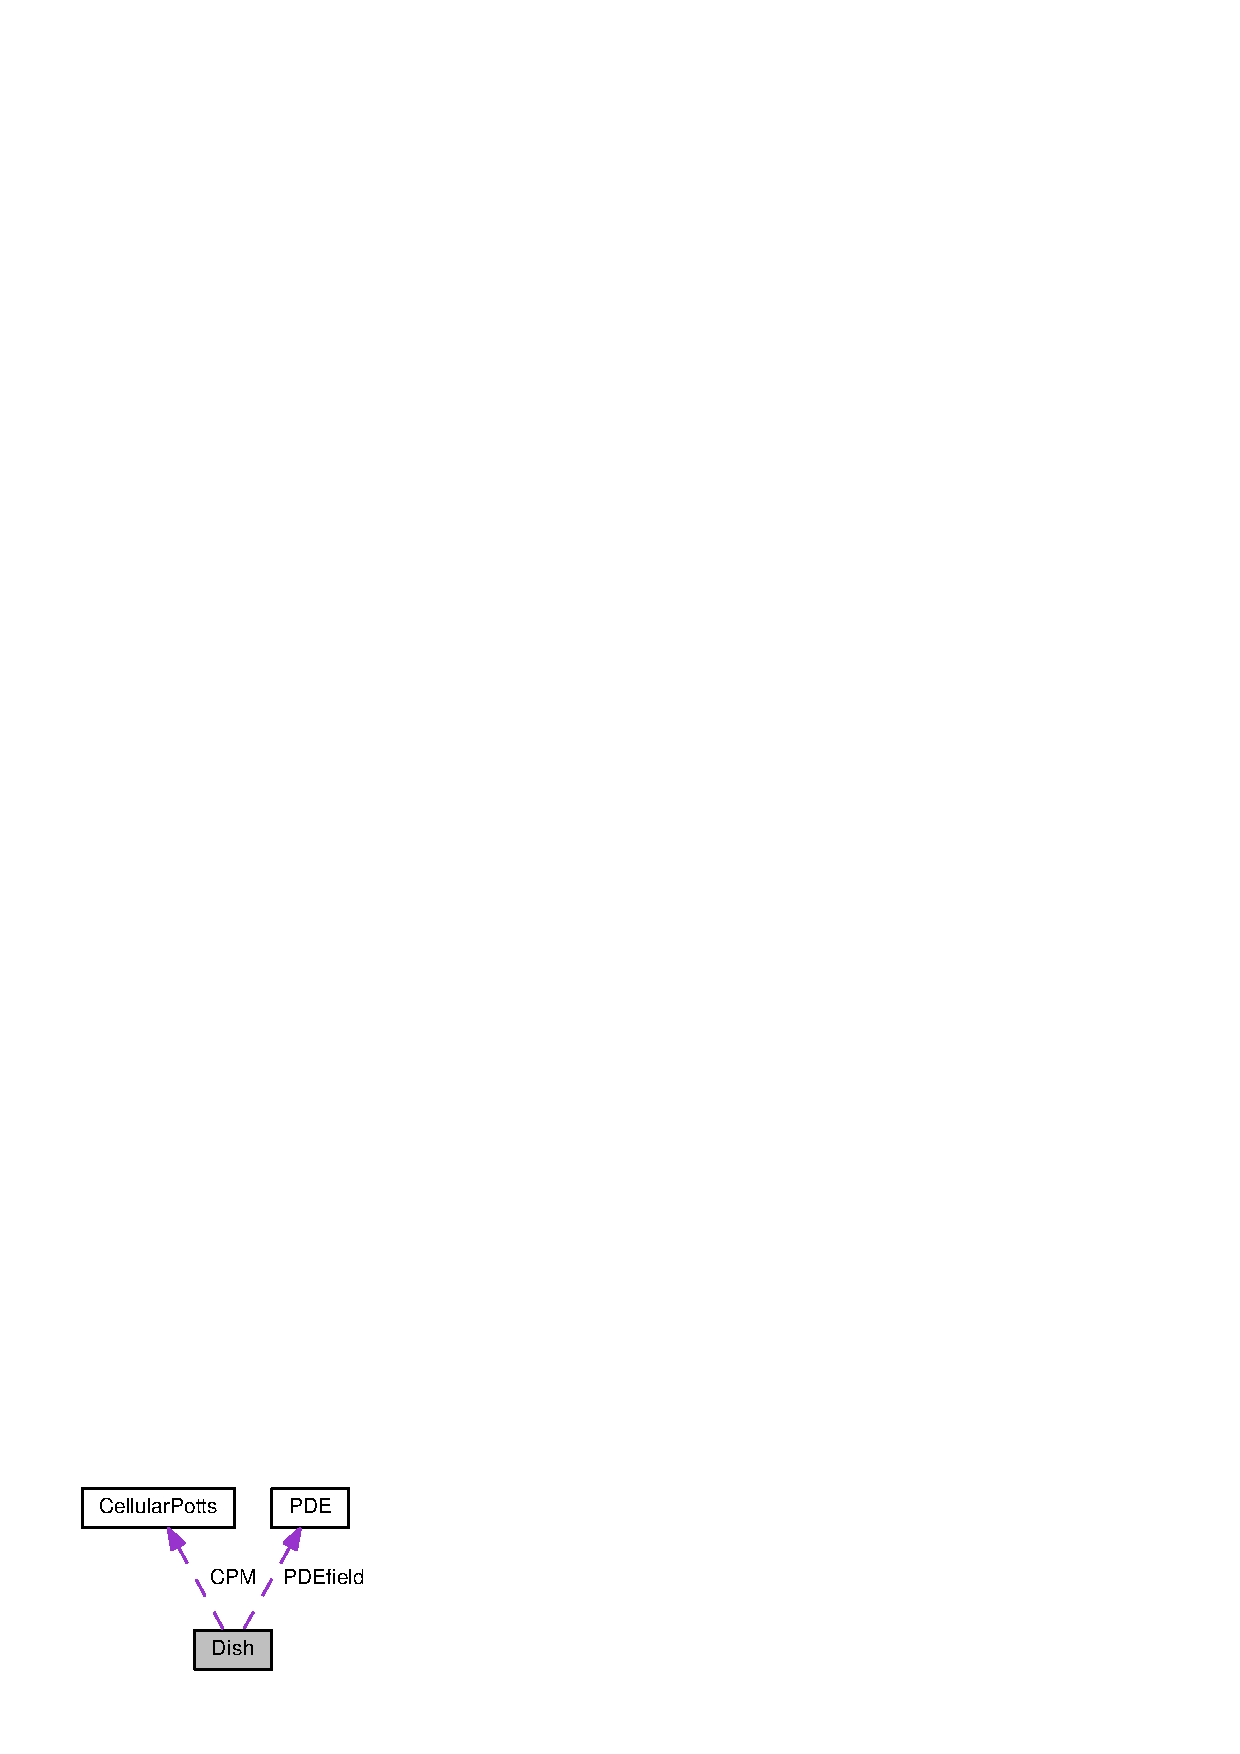
\includegraphics[width=179pt]{classDish__coll__graph}
\end{center}
\end{figure}
\subsection*{Public Member Functions}
\begin{DoxyCompactItemize}
\item 
{\bf Dish} (void)
\item 
void {\bf Init} (void)
\begin{DoxyCompactList}\small\item\em Init defines the initial state of the virtual cell culture. \end{DoxyCompactList}\item 
void {\bf Constructor\-Body} (void)
\item 
virtual {\bf $\sim$\-Dish} ()
\item 
void {\bf Plot} ({\bf Graphics} $\ast$g)
\begin{DoxyCompactList}\small\item\em Plot the \doxyref{Dish}{p.}{classDish} to graphics window g. \end{DoxyCompactList}\item 
int {\bf Zygote\-Area} (void) const 
\item 
int {\bf Time} (void) const 
\begin{DoxyCompactList}\small\item\em Returns the number of completed Monte Carlo Steps. \end{DoxyCompactList}\item 
int {\bf Count\-Cells} (void) const 
\begin{DoxyCompactList}\small\item\em Returns the number of cells in the dish, excluding apoptosed cells. \end{DoxyCompactList}\item 
void {\bf Cell\-Growth\-And\-Division} (void)
\begin{DoxyCompactList}\small\item\em Stretched induced cell growth and division. \end{DoxyCompactList}\item 
int {\bf Area} (void) const 
\begin{DoxyCompactList}\small\item\em . Returns the summed area of all cells in the dish \end{DoxyCompactList}\item 
int {\bf Target\-Area} (void) const 
\begin{DoxyCompactList}\small\item\em Returns the summed of all cells target area in the dish. \end{DoxyCompactList}\item 
int {\bf Size\-X} (void)
\begin{DoxyCompactList}\small\item\em Returns the horizontal size of the dish. \end{DoxyCompactList}\item 
int {\bf Size\-Y} (void)
\begin{DoxyCompactList}\small\item\em Returns the horizontal size of the dish. \end{DoxyCompactList}\item 
{\bf Cell} \& {\bf get\-Cell} (int c)
\begin{DoxyCompactList}\small\item\em Returns a reference to cell number \char`\"{}c\char`\"{}. \end{DoxyCompactList}\item 
void {\bf Clear\-Grads} (void)
\item 
void {\bf Measure\-Chem\-Concentrations} (void)
\end{DoxyCompactItemize}
\subsection*{Public Attributes}
\begin{DoxyCompactItemize}
\item 
{\bf P\-D\-E} $\ast$ {\bf P\-D\-Efield}
\item 
{\bf Cellular\-Potts} $\ast$ {\bf C\-P\-M}
\end{DoxyCompactItemize}
\subsection*{Protected Member Functions}
\begin{DoxyCompactItemize}
\item 
void {\bf Set\-Cell\-Owner} ({\bf Cell} \&which\-\_\-cell)
\begin{DoxyCompactList}\small\item\em Assign a the cell to the current \doxyref{Dish}{p.}{classDish}. \end{DoxyCompactList}\end{DoxyCompactItemize}
\subsection*{Protected Attributes}
\begin{DoxyCompactItemize}
\item 
std\-::vector$<$ {\bf Cell} $>$ {\bf cell}
\begin{DoxyCompactList}\small\item\em The cells in the Petri dish; accessible to derived classes. \end{DoxyCompactList}\end{DoxyCompactItemize}
\subsection*{Friends}
\begin{DoxyCompactItemize}
\item 
class {\bf Info}
\end{DoxyCompactItemize}


\subsection{Detailed Description}
The virtual Petri dish. 

Hosts the cells with states and the C\-A-\/plane. 

\subsection{Constructor \& Destructor Documentation}
\index{Dish@{Dish}!Dish@{Dish}}
\index{Dish@{Dish}!Dish@{Dish}}
\subsubsection[{Dish}]{\setlength{\rightskip}{0pt plus 5cm}Dish\-::\-Dish (
\begin{DoxyParamCaption}
\item[{void}]{}
\end{DoxyParamCaption}
)}\label{classDish_af0f707b604af60f65683fb27a0e73de2}


References Parameter\-::n\-\_\-chem, Parameter\-::sizex, Parameter\-::sizey, and Parameter\-::target\-\_\-area.

\index{Dish@{Dish}!$\sim$\-Dish@{$\sim$\-Dish}}
\index{$\sim$\-Dish@{$\sim$\-Dish}!Dish@{Dish}}
\subsubsection[{$\sim$\-Dish}]{\setlength{\rightskip}{0pt plus 5cm}Dish\-::$\sim$\-Dish (
\begin{DoxyParamCaption}
{}
\end{DoxyParamCaption}
)\hspace{0.3cm}{\ttfamily [virtual]}}\label{classDish_a6ea34b164531bdf29a57e3b4060af111}


\subsection{Member Function Documentation}
\index{Dish@{Dish}!Area@{Area}}
\index{Area@{Area}!Dish@{Dish}}
\subsubsection[{Area}]{\setlength{\rightskip}{0pt plus 5cm}int Dish\-::\-Area (
\begin{DoxyParamCaption}
\item[{void}]{}
\end{DoxyParamCaption}
) const}\label{classDish_a575eb2325f18ed4cb4bd04912ebe0658}


. Returns the summed area of all cells in the dish 

\index{Dish@{Dish}!Cell\-Growth\-And\-Division@{Cell\-Growth\-And\-Division}}
\index{Cell\-Growth\-And\-Division@{Cell\-Growth\-And\-Division}!Dish@{Dish}}
\subsubsection[{Cell\-Growth\-And\-Division}]{\setlength{\rightskip}{0pt plus 5cm}void Dish\-::\-Cell\-Growth\-And\-Division (
\begin{DoxyParamCaption}
\item[{void}]{}
\end{DoxyParamCaption}
)}\label{classDish_a41c5667d06a94812b78a83355b266770}


Stretched induced cell growth and division. 

See Hogeweg (2000), Journal of Theoretical Biology.

Find stretched cells, and increase their target area. Find enlarged cells, and divide them. 

References Cell\-::\-Increment\-Target\-Area().

\index{Dish@{Dish}!Clear\-Grads@{Clear\-Grads}}
\index{Clear\-Grads@{Clear\-Grads}!Dish@{Dish}}
\subsubsection[{Clear\-Grads}]{\setlength{\rightskip}{0pt plus 5cm}void Dish\-::\-Clear\-Grads (
\begin{DoxyParamCaption}
\item[{void}]{}
\end{DoxyParamCaption}
)}\label{classDish_acf2e4c3b278746cdeef77fe4e4ed16c3}
\index{Dish@{Dish}!Constructor\-Body@{Constructor\-Body}}
\index{Constructor\-Body@{Constructor\-Body}!Dish@{Dish}}
\subsubsection[{Constructor\-Body}]{\setlength{\rightskip}{0pt plus 5cm}void Dish\-::\-Constructor\-Body (
\begin{DoxyParamCaption}
\item[{void}]{}
\end{DoxyParamCaption}
)}\label{classDish_a7180a1e281da830a4d64a630ce728017}


References Cell\-::maxsigma.

\index{Dish@{Dish}!Count\-Cells@{Count\-Cells}}
\index{Count\-Cells@{Count\-Cells}!Dish@{Dish}}
\subsubsection[{Count\-Cells}]{\setlength{\rightskip}{0pt plus 5cm}int Dish\-::\-Count\-Cells (
\begin{DoxyParamCaption}
\item[{void}]{}
\end{DoxyParamCaption}
) const}\label{classDish_a0728f035933718f1f08d1b07d8e77dd1}


Returns the number of cells in the dish, excluding apoptosed cells. 

\index{Dish@{Dish}!get\-Cell@{get\-Cell}}
\index{get\-Cell@{get\-Cell}!Dish@{Dish}}
\subsubsection[{get\-Cell}]{\setlength{\rightskip}{0pt plus 5cm}{\bf Cell}\& Dish\-::get\-Cell (
\begin{DoxyParamCaption}
\item[{int}]{c}
\end{DoxyParamCaption}
)\hspace{0.3cm}{\ttfamily [inline]}}\label{classDish_a68612ff30d41a691d9b808474685b940}


Returns a reference to cell number \char`\"{}c\char`\"{}. 



References cell.

\index{Dish@{Dish}!Init@{Init}}
\index{Init@{Init}!Dish@{Dish}}
\subsubsection[{Init}]{\setlength{\rightskip}{0pt plus 5cm}void Dish\-::\-Init (
\begin{DoxyParamCaption}
\item[{void}]{}
\end{DoxyParamCaption}
)}\label{classDish_aae99b3ba84abb07cacdaba97e35844bd}


Init defines the initial state of the virtual cell culture. 

Define \doxyref{Init()}{p.}{classDish_aae99b3ba84abb07cacdaba97e35844bd} in your main file describing the simulation set up, within the block I\-N\-I\-T \{ \}. See for examples \doxyref{vessel.\-cpp}{p.}{vessel_8cpp} and \doxyref{sorting.\-cpp}{p.}{sorting_8cpp}. \index{Dish@{Dish}!Measure\-Chem\-Concentrations@{Measure\-Chem\-Concentrations}}
\index{Measure\-Chem\-Concentrations@{Measure\-Chem\-Concentrations}!Dish@{Dish}}
\subsubsection[{Measure\-Chem\-Concentrations}]{\setlength{\rightskip}{0pt plus 5cm}void Dish\-::\-Measure\-Chem\-Concentrations (
\begin{DoxyParamCaption}
\item[{void}]{}
\end{DoxyParamCaption}
)}\label{classDish_a8590b706fcf6bc66b52004b0289d1353}


References Cell\-::\-Area(), Cell\-::chem, and Parameter\-::n\-\_\-chem.

\index{Dish@{Dish}!Plot@{Plot}}
\index{Plot@{Plot}!Dish@{Dish}}
\subsubsection[{Plot}]{\setlength{\rightskip}{0pt plus 5cm}void Dish\-::\-Plot (
\begin{DoxyParamCaption}
\item[{{\bf Graphics} $\ast$}]{g}
\end{DoxyParamCaption}
)}\label{classDish_aac30508ed8fdc83a659451f738786ee6}


Plot the \doxyref{Dish}{p.}{classDish} to graphics window g. 

Simply calls C\-P\-M-\/$>$Plot. \index{Dish@{Dish}!Set\-Cell\-Owner@{Set\-Cell\-Owner}}
\index{Set\-Cell\-Owner@{Set\-Cell\-Owner}!Dish@{Dish}}
\subsubsection[{Set\-Cell\-Owner}]{\setlength{\rightskip}{0pt plus 5cm}void Dish\-::\-Set\-Cell\-Owner (
\begin{DoxyParamCaption}
\item[{{\bf Cell} \&}]{which\-\_\-cell}
\end{DoxyParamCaption}
)\hspace{0.3cm}{\ttfamily [protected]}}\label{classDish_a1e73feecedc005f2782aaf2e37ab2df6}


Assign a the cell to the current \doxyref{Dish}{p.}{classDish}. 



References Cell\-::owner.

\index{Dish@{Dish}!Size\-X@{Size\-X}}
\index{Size\-X@{Size\-X}!Dish@{Dish}}
\subsubsection[{Size\-X}]{\setlength{\rightskip}{0pt plus 5cm}int Dish\-::\-Size\-X (
\begin{DoxyParamCaption}
\item[{void}]{}
\end{DoxyParamCaption}
)}\label{classDish_a403577ee8ef78a8cb7b2b4d888167649}


Returns the horizontal size of the dish. 

\index{Dish@{Dish}!Size\-Y@{Size\-Y}}
\index{Size\-Y@{Size\-Y}!Dish@{Dish}}
\subsubsection[{Size\-Y}]{\setlength{\rightskip}{0pt plus 5cm}int Dish\-::\-Size\-Y (
\begin{DoxyParamCaption}
\item[{void}]{}
\end{DoxyParamCaption}
)}\label{classDish_aee8463a854b44635bb7917c39af70040}


Returns the horizontal size of the dish. 

\index{Dish@{Dish}!Target\-Area@{Target\-Area}}
\index{Target\-Area@{Target\-Area}!Dish@{Dish}}
\subsubsection[{Target\-Area}]{\setlength{\rightskip}{0pt plus 5cm}int Dish\-::\-Target\-Area (
\begin{DoxyParamCaption}
\item[{void}]{}
\end{DoxyParamCaption}
) const}\label{classDish_ad7630eed11b5bd545a4ebfc736988b86}


Returns the summed of all cells target area in the dish. 

\index{Dish@{Dish}!Time@{Time}}
\index{Time@{Time}!Dish@{Dish}}
\subsubsection[{Time}]{\setlength{\rightskip}{0pt plus 5cm}int Dish\-::\-Time (
\begin{DoxyParamCaption}
\item[{void}]{}
\end{DoxyParamCaption}
) const}\label{classDish_a98a644d8e6a7a79111e9203359a3ee0a}


Returns the number of completed Monte Carlo Steps. 



Referenced by Cell\-::\-Cell\-Birth().

\index{Dish@{Dish}!Zygote\-Area@{Zygote\-Area}}
\index{Zygote\-Area@{Zygote\-Area}!Dish@{Dish}}
\subsubsection[{Zygote\-Area}]{\setlength{\rightskip}{0pt plus 5cm}int Dish\-::\-Zygote\-Area (
\begin{DoxyParamCaption}
\item[{void}]{}
\end{DoxyParamCaption}
) const}\label{classDish_aed5a6aa8f6a5cc4e1f301fb2b201a685}


\subsection{Friends And Related Function Documentation}
\index{Dish@{Dish}!Info@{Info}}
\index{Info@{Info}!Dish@{Dish}}
\subsubsection[{Info}]{\setlength{\rightskip}{0pt plus 5cm}friend class {\bf Info}\hspace{0.3cm}{\ttfamily [friend]}}\label{classDish_a4838ff865b8d8625c61d208a420f8212}


\subsection{Member Data Documentation}
\index{Dish@{Dish}!cell@{cell}}
\index{cell@{cell}!Dish@{Dish}}
\subsubsection[{cell}]{\setlength{\rightskip}{0pt plus 5cm}std\-::vector$<${\bf Cell}$>$ Dish\-::cell\hspace{0.3cm}{\ttfamily [protected]}}\label{classDish_a033f004ac525f6edbf0af46819acf707}


The cells in the Petri dish; accessible to derived classes. 



Referenced by get\-Cell().

\index{Dish@{Dish}!C\-P\-M@{C\-P\-M}}
\index{C\-P\-M@{C\-P\-M}!Dish@{Dish}}
\subsubsection[{C\-P\-M}]{\setlength{\rightskip}{0pt plus 5cm}{\bf Cellular\-Potts}$\ast$ Dish\-::\-C\-P\-M}\label{classDish_a61c008708298cb9c949546af9ce2c98d}
\index{Dish@{Dish}!P\-D\-Efield@{P\-D\-Efield}}
\index{P\-D\-Efield@{P\-D\-Efield}!Dish@{Dish}}
\subsubsection[{P\-D\-Efield}]{\setlength{\rightskip}{0pt plus 5cm}{\bf P\-D\-E}$\ast$ Dish\-::\-P\-D\-Efield}\label{classDish_a096ba06e44f54deb7c9b16669876cd2c}


The documentation for this class was generated from the following files\-:\begin{DoxyCompactItemize}
\item 
{\bf dish.\-h}\item 
{\bf dish.\-cpp}\end{DoxyCompactItemize}

\section{Graphics Class Reference}
\label{classGraphics}\index{Graphics@{Graphics}}


A\-P\-I for \doxyref{Graphics}{p.}{classGraphics} windows.  




{\ttfamily \#include $<$graph.\-h$>$}



Inheritance diagram for Graphics\-:
\nopagebreak
\begin{figure}[H]
\begin{center}
\leavevmode
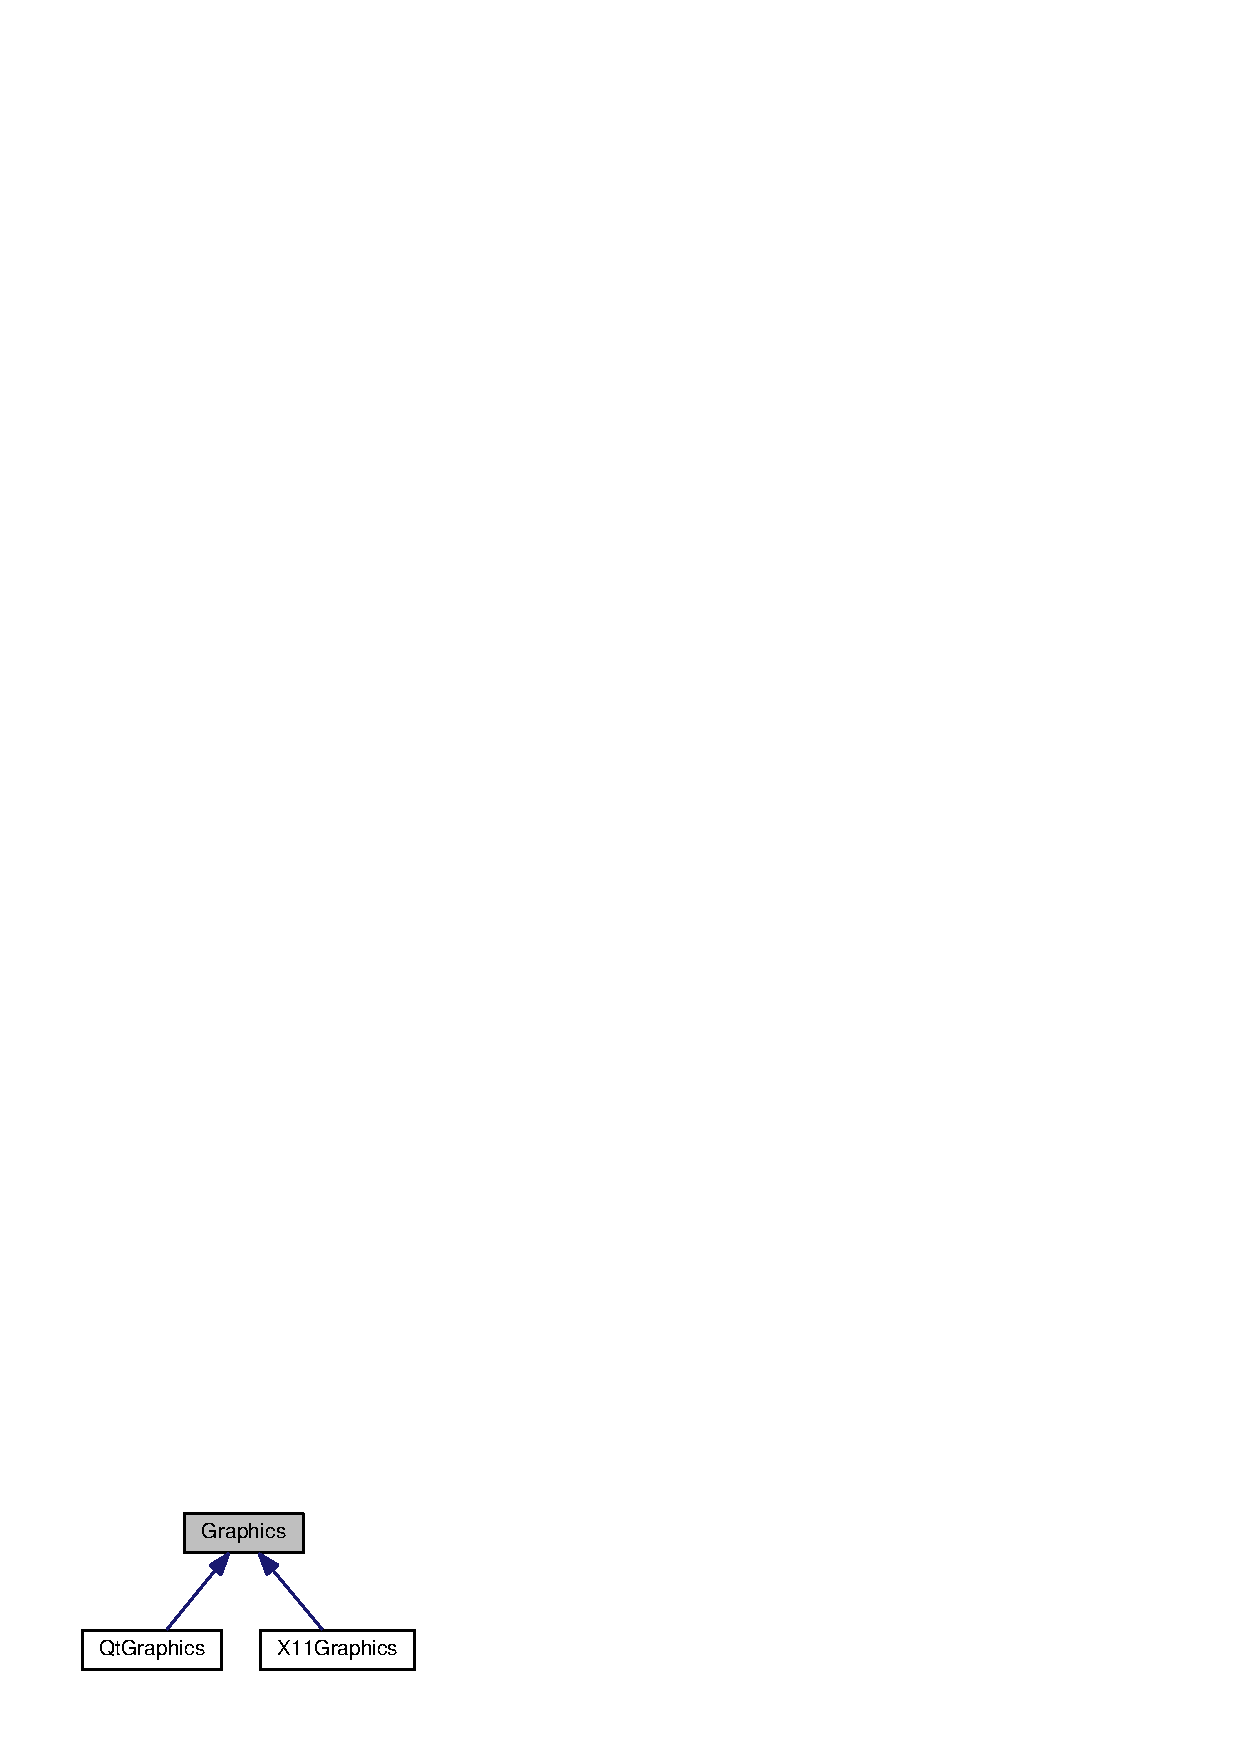
\includegraphics[width=203pt]{classGraphics__inherit__graph}
\end{center}
\end{figure}
\subsection*{Public Member Functions}
\begin{DoxyCompactItemize}
\item 
virtual {\bf $\sim$\-Graphics} (void)
\item 
virtual void {\bf Begin\-Scene} (void)
\begin{DoxyCompactList}\small\item\em \doxyref{Begin\-Scene()}{p.}{classGraphics_afc5b72e258d26775418c72c78d078e4b} must be called before calling drawing functions. \end{DoxyCompactList}\item 
virtual void {\bf End\-Scene} (void)
\begin{DoxyCompactList}\small\item\em \doxyref{End\-Scene()}{p.}{classGraphics_a9f97b7c6506dcba845a1da457398fa90} must be called to flush the drawing buffer and display the scene. \end{DoxyCompactList}\item 
virtual void {\bf Point} (int color, int x, int y)=0
\begin{DoxyCompactList}\small\item\em Plot a point in the \doxyref{Graphics}{p.}{classGraphics} window. \end{DoxyCompactList}\item 
virtual void {\bf Line} (int x1, int y1, int x2, int y2, int colour)=0
\begin{DoxyCompactList}\small\item\em Draws a line (obviously... \-:-\/) \end{DoxyCompactList}\item 
virtual int {\bf Get\-X\-Y\-Coo} (int $\ast$X, int $\ast$Y)=0
\begin{DoxyCompactList}\small\item\em Probes the Window for user interaction, with mouse or keyboard. \end{DoxyCompactList}\item 
virtual int {\bf X\-Field} (void) const 
\begin{DoxyCompactList}\small\item\em Returns the width of the \doxyref{Graphics}{p.}{classGraphics} window, in pixels. \end{DoxyCompactList}\item 
virtual int {\bf Y\-Field} (void) const 
\begin{DoxyCompactList}\small\item\em Returns the height of the \doxyref{Graphics}{p.}{classGraphics} window, in pixels. \end{DoxyCompactList}\item 
virtual void {\bf Write} (char $\ast$fname, int quality=-\/1)=0
\begin{DoxyCompactList}\small\item\em Writes the Image to a file. \end{DoxyCompactList}\item 
virtual void {\bf Time\-Step} (void)
\begin{DoxyCompactList}\small\item\em Implement this member function in your simulation code. \end{DoxyCompactList}\item 
virtual void {\bf Field} (const int $\ast$$\ast$f, int mag=1)
\begin{DoxyCompactList}\small\item\em Plots a field of values given by $\ast$$\ast$f, using color coding given by colormap file. \end{DoxyCompactList}\end{DoxyCompactItemize}


\subsection{Detailed Description}
A\-P\-I for \doxyref{Graphics}{p.}{classGraphics} windows. 

No implementation here. Implemented by \doxyref{X11\-Graphics}{p.}{classX11Graphics} and \doxyref{Qt\-Graphics}{p.}{classQtGraphics}. 

\subsection{Constructor \& Destructor Documentation}
\index{Graphics@{Graphics}!$\sim$\-Graphics@{$\sim$\-Graphics}}
\index{$\sim$\-Graphics@{$\sim$\-Graphics}!Graphics@{Graphics}}
\subsubsection[{$\sim$\-Graphics}]{\setlength{\rightskip}{0pt plus 5cm}virtual Graphics\-::$\sim$\-Graphics (
\begin{DoxyParamCaption}
\item[{void}]{}
\end{DoxyParamCaption}
)\hspace{0.3cm}{\ttfamily [inline]}, {\ttfamily [virtual]}}\label{classGraphics_ae6b6c5a05e2fe1f05c871f1eb7e8ac19}


\subsection{Member Function Documentation}
\index{Graphics@{Graphics}!Begin\-Scene@{Begin\-Scene}}
\index{Begin\-Scene@{Begin\-Scene}!Graphics@{Graphics}}
\subsubsection[{Begin\-Scene}]{\setlength{\rightskip}{0pt plus 5cm}virtual void Graphics\-::\-Begin\-Scene (
\begin{DoxyParamCaption}
\item[{void}]{}
\end{DoxyParamCaption}
)\hspace{0.3cm}{\ttfamily [inline]}, {\ttfamily [virtual]}}\label{classGraphics_afc5b72e258d26775418c72c78d078e4b}


\doxyref{Begin\-Scene()}{p.}{classGraphics_afc5b72e258d26775418c72c78d078e4b} must be called before calling drawing functions. 



Reimplemented in {\bf X11\-Graphics} \doxyref{}{p.}{classX11Graphics_af90168e2537eb714dd0d916a2c543f74}, and {\bf Qt\-Graphics} \doxyref{}{p.}{classQtGraphics_afd6200f3cbb931d811791f7683425f84}.

\index{Graphics@{Graphics}!End\-Scene@{End\-Scene}}
\index{End\-Scene@{End\-Scene}!Graphics@{Graphics}}
\subsubsection[{End\-Scene}]{\setlength{\rightskip}{0pt plus 5cm}virtual void Graphics\-::\-End\-Scene (
\begin{DoxyParamCaption}
\item[{void}]{}
\end{DoxyParamCaption}
)\hspace{0.3cm}{\ttfamily [inline]}, {\ttfamily [virtual]}}\label{classGraphics_a9f97b7c6506dcba845a1da457398fa90}


\doxyref{End\-Scene()}{p.}{classGraphics_a9f97b7c6506dcba845a1da457398fa90} must be called to flush the drawing buffer and display the scene. 



Reimplemented in {\bf X11\-Graphics} \doxyref{}{p.}{classX11Graphics_aeafb2bf394ef9dfd3aa9b390d2b21d7a}, and {\bf Qt\-Graphics} \doxyref{}{p.}{classQtGraphics_a937c2227c5d121f56f9651d3aeccc27a}.

\index{Graphics@{Graphics}!Field@{Field}}
\index{Field@{Field}!Graphics@{Graphics}}
\subsubsection[{Field}]{\setlength{\rightskip}{0pt plus 5cm}virtual void Graphics\-::\-Field (
\begin{DoxyParamCaption}
\item[{const int $\ast$$\ast$}]{f, }
\item[{int}]{mag = {\ttfamily 1}}
\end{DoxyParamCaption}
)\hspace{0.3cm}{\ttfamily [inline]}, {\ttfamily [virtual]}}\label{classGraphics_a22105e059337daabadfa68838811099f}


Plots a field of values given by $\ast$$\ast$f, using color coding given by colormap file. 

Only implemented in \doxyref{X11\-Graphics}{p.}{classX11Graphics}. No checks. Usage not recommended.


\begin{DoxyParams}{Parameters}
{\em f} & Double pointer to array of integers, giving color indices using standard colormap ('default.\-ctb'). \\
\hline
{\em mag} & magnification factor. \\
\hline
\end{DoxyParams}


Reimplemented in {\bf X11\-Graphics} \doxyref{}{p.}{classX11Graphics_a4ba01ab14685f860af345b4ac17f3339}.

\index{Graphics@{Graphics}!Get\-X\-Y\-Coo@{Get\-X\-Y\-Coo}}
\index{Get\-X\-Y\-Coo@{Get\-X\-Y\-Coo}!Graphics@{Graphics}}
\subsubsection[{Get\-X\-Y\-Coo}]{\setlength{\rightskip}{0pt plus 5cm}virtual int Graphics\-::\-Get\-X\-Y\-Coo (
\begin{DoxyParamCaption}
\item[{int $\ast$}]{X, }
\item[{int $\ast$}]{Y}
\end{DoxyParamCaption}
)\hspace{0.3cm}{\ttfamily [pure virtual]}}\label{classGraphics_a39257f929b38739ed42e8d463c4f42c3}


Probes the Window for user interaction, with mouse or keyboard. 

This function should return immediately, and return 0 if there was no user interaction.


\begin{DoxyParams}{Parameters}
{\em $\ast$\-X,$\ast$\-Y} & Pointer where the clicked coordinate will be stored. \\
\hline
\end{DoxyParams}


Implemented in {\bf X11\-Graphics} \doxyref{}{p.}{classX11Graphics_a2d3f6a3d4b3f0131dbfb9253d51f0ebc}, and {\bf Qt\-Graphics} \doxyref{}{p.}{classQtGraphics_a497ca587ebbac0336589066147de3ab5}.



Referenced by Info\-::\-Click\-Cell().

\index{Graphics@{Graphics}!Line@{Line}}
\index{Line@{Line}!Graphics@{Graphics}}
\subsubsection[{Line}]{\setlength{\rightskip}{0pt plus 5cm}virtual void Graphics\-::\-Line (
\begin{DoxyParamCaption}
\item[{int}]{x1, }
\item[{int}]{y1, }
\item[{int}]{x2, }
\item[{int}]{y2, }
\item[{int}]{colour}
\end{DoxyParamCaption}
)\hspace{0.3cm}{\ttfamily [pure virtual]}}\label{classGraphics_a8e049566ac4cf6168b04f0f8be7a9820}


Draws a line (obviously... \-:-\/) 


\begin{DoxyParams}{Parameters}
{\em x1,y1} & First coordinate pair. \\
\hline
{\em x2,y2} & Second coordinate pair. \\
\hline
{\em color} & Color of the line, as given in the colormap file \char`\"{}default.\-ctb\char`\"{}. \\
\hline
\end{DoxyParams}


Implemented in {\bf X11\-Graphics} \doxyref{}{p.}{classX11Graphics_a8126d246d7925babf273df1fa948466d}, and {\bf Qt\-Graphics} \doxyref{}{p.}{classQtGraphics_a4ca1bd37d041d0741fd4c82e0705511b}.



Referenced by Cellular\-Potts\-::\-Draw\-Convex\-Hull(), P\-D\-E\-::\-Plot\-Vector\-Field(), and Cellular\-Potts\-::\-Show\-Directions().

\index{Graphics@{Graphics}!Point@{Point}}
\index{Point@{Point}!Graphics@{Graphics}}
\subsubsection[{Point}]{\setlength{\rightskip}{0pt plus 5cm}virtual void Graphics\-::\-Point (
\begin{DoxyParamCaption}
\item[{int}]{color, }
\item[{int}]{x, }
\item[{int}]{y}
\end{DoxyParamCaption}
)\hspace{0.3cm}{\ttfamily [pure virtual]}}\label{classGraphics_a123e1b2c757c39bf329517af332c24eb}


Plot a point in the \doxyref{Graphics}{p.}{classGraphics} window. 


\begin{DoxyParams}{Parameters}
{\em color} & Color index, as defined in colormap file \char`\"{}default.\-ctb\char`\"{}, which should be in the same directory as the executable. \\
\hline
{\em x,y} & Coordinate of point, in \doxyref{Graphics}{p.}{classGraphics} coordinates (typically twice as large as the cellular automata coordinates). \\
\hline
\end{DoxyParams}


Implemented in {\bf X11\-Graphics} \doxyref{}{p.}{classX11Graphics_aac47663836332028e6a382af6a2c622c}, and {\bf Qt\-Graphics} \doxyref{}{p.}{classQtGraphics_ad02ff8ba69d13148f79afd516563b822}.



Referenced by conrec(), P\-D\-E\-::\-Plot(), Cellular\-Potts\-::\-Plot\-Sigma(), and Cellular\-Potts\-::\-Search\-Nand\-Plot().

\index{Graphics@{Graphics}!Time\-Step@{Time\-Step}}
\index{Time\-Step@{Time\-Step}!Graphics@{Graphics}}
\subsubsection[{Time\-Step}]{\setlength{\rightskip}{0pt plus 5cm}virtual void Graphics\-::\-Time\-Step (
\begin{DoxyParamCaption}
\item[{void}]{}
\end{DoxyParamCaption}
)\hspace{0.3cm}{\ttfamily [inline]}, {\ttfamily [virtual]}}\label{classGraphics_aa1b61fa6f6bc50aceff6f320ce5b9be2}


Implement this member function in your simulation code. 

Include all actions that should be carried out during a simulation step, including \doxyref{P\-D\-E}{p.}{classPDE} and C\-P\-M simulation steps. See the included examples (\doxyref{vessel.\-cpp}{p.}{vessel_8cpp}, \doxyref{sorting.\-cpp}{p.}{sorting_8cpp}) for more information. 

Reimplemented in {\bf X11\-Graphics} \doxyref{}{p.}{classX11Graphics_a44567816671f4055f76999432509d505}, and {\bf Qt\-Graphics} \doxyref{}{p.}{classQtGraphics_a6c3e54b681404b550417628910557ade}.

\index{Graphics@{Graphics}!Write@{Write}}
\index{Write@{Write}!Graphics@{Graphics}}
\subsubsection[{Write}]{\setlength{\rightskip}{0pt plus 5cm}virtual void Graphics\-::\-Write (
\begin{DoxyParamCaption}
\item[{char $\ast$}]{fname, }
\item[{int}]{quality = {\ttfamily -\/1}}
\end{DoxyParamCaption}
)\hspace{0.3cm}{\ttfamily [pure virtual]}}\label{classGraphics_af98a333b8be25817669e615b1cd6c73d}


Writes the Image to a file. 

File format is inferred from file extension. Currently only P\-N\-G is supported by the X-\/\-Windows implementation; the Qt-\/implentation supports all formats supported by Qt.


\begin{DoxyParams}{Parameters}
{\em fname} & File name with standard image file extension (e.\-g. png). \\
\hline
{\em quality} & Quality of J\-P\-E\-G images, defaults to -\/1 (no value provided). \\
\hline
\end{DoxyParams}


Implemented in {\bf X11\-Graphics} \doxyref{}{p.}{classX11Graphics_a82f63efbb9969b69a59c850356d219d3}, and {\bf Qt\-Graphics} \doxyref{}{p.}{classQtGraphics_a2b3ae718854987c2746f8d723fbf3fa6}.

\index{Graphics@{Graphics}!X\-Field@{X\-Field}}
\index{X\-Field@{X\-Field}!Graphics@{Graphics}}
\subsubsection[{X\-Field}]{\setlength{\rightskip}{0pt plus 5cm}virtual int Graphics\-::\-X\-Field (
\begin{DoxyParamCaption}
\item[{void}]{}
\end{DoxyParamCaption}
) const\hspace{0.3cm}{\ttfamily [inline]}, {\ttfamily [virtual]}}\label{classGraphics_a57a2d92f0744fe35be0a712803178a4f}


Returns the width of the \doxyref{Graphics}{p.}{classGraphics} window, in pixels. 



Reimplemented in {\bf X11\-Graphics} \doxyref{}{p.}{classX11Graphics_a16e04390d5a23f68e5556504460f55df}, and {\bf Qt\-Graphics} \doxyref{}{p.}{classQtGraphics_ae18cae9c5ade06e287f40190b919639d}.

\index{Graphics@{Graphics}!Y\-Field@{Y\-Field}}
\index{Y\-Field@{Y\-Field}!Graphics@{Graphics}}
\subsubsection[{Y\-Field}]{\setlength{\rightskip}{0pt plus 5cm}virtual int Graphics\-::\-Y\-Field (
\begin{DoxyParamCaption}
\item[{void}]{}
\end{DoxyParamCaption}
) const\hspace{0.3cm}{\ttfamily [inline]}, {\ttfamily [virtual]}}\label{classGraphics_ad9df13b4bb136c8c5ca802ec8f382e47}


Returns the height of the \doxyref{Graphics}{p.}{classGraphics} window, in pixels. 



Reimplemented in {\bf X11\-Graphics} \doxyref{}{p.}{classX11Graphics_ab0b8df7d9fad28f5a377ca45894de113}, and {\bf Qt\-Graphics} \doxyref{}{p.}{classQtGraphics_a9945f6ee5fa3ddf649a5a4ac52785356}.



The documentation for this class was generated from the following file\-:\begin{DoxyCompactItemize}
\item 
{\bf graph.\-h}\end{DoxyCompactItemize}

\section{Info Class Reference}
\label{classInfo}\index{Info@{Info}}


Enables interactive querying of the simulation.  




{\ttfamily \#include $<$info.\-h$>$}

\subsection*{Public Member Functions}
\begin{DoxyCompactItemize}
\item 
{\bf Info} ({\bf Dish} \&dish, {\bf Graphics} \&graphics, std\-::ostream \&out=std\-::cout)
\begin{DoxyCompactList}\small\item\em Constructs and \doxyref{Info}{p.}{classInfo} class dish with specified graphics window. \end{DoxyCompactList}\item 
void {\bf Menu} (void)
\begin{DoxyCompactList}\small\item\em Reads out key presses in the \doxyref{Graphics}{p.}{classGraphics} window and interprets them. \end{DoxyCompactList}\item 
void {\bf Write\-C\-O\-M} (int cell\-\_\-id, std\-::ostream \&out=std\-::cout)
\begin{DoxyCompactList}\small\item\em Writes center of mass of cell \char`\"{}cell\-\_\-id\char`\"{} to stream out. \end{DoxyCompactList}\item 
{\bf Cell} \& {\bf Click\-Cell} ({\bf Graphics} $\ast$g)
\begin{DoxyCompactList}\small\item\em Waits until the user clicks a cell and returns a reference to it. \end{DoxyCompactList}\end{DoxyCompactItemize}


\subsection{Detailed Description}
Enables interactive querying of the simulation. 

Only using key presses, to be defined in \doxyref{Info\-::\-Menu()}{p.}{classInfo_af684a1acfe0ed9c185bbc6a886856f2f}.

Right-\/click menu in future Qt-\/linked versions? 

\subsection{Constructor \& Destructor Documentation}
\index{Info@{Info}!Info@{Info}}
\index{Info@{Info}!Info@{Info}}
\subsubsection[{Info}]{\setlength{\rightskip}{0pt plus 5cm}Info\-::\-Info (
\begin{DoxyParamCaption}
\item[{{\bf Dish} \&}]{dish, }
\item[{{\bf Graphics} \&}]{graphics, }
\item[{std\-::ostream \&}]{out = {\ttfamily std\-:\-:cout}}
\end{DoxyParamCaption}
)}\label{classInfo_a11adc40bc41bed325a30dc5f75d4f813}


Constructs and \doxyref{Info}{p.}{classInfo} class dish with specified graphics window. 


\begin{DoxyParams}{Parameters}
{\em dish} & The virtual Petri dish to query. \\
\hline
{\em graphics} & The \doxyref{Graphics}{p.}{classGraphics} window displaying the dish. \\
\hline
{\em out} & (optional) Stream into which info is written. Default\-: console. \\
\hline
\end{DoxyParams}


References Info().



Referenced by Info().



\subsection{Member Function Documentation}
\index{Info@{Info}!Click\-Cell@{Click\-Cell}}
\index{Click\-Cell@{Click\-Cell}!Info@{Info}}
\subsubsection[{Click\-Cell}]{\setlength{\rightskip}{0pt plus 5cm}{\bf Cell} \& Info\-::\-Click\-Cell (
\begin{DoxyParamCaption}
\item[{{\bf Graphics} $\ast$}]{g}
\end{DoxyParamCaption}
)}\label{classInfo_ad66d701be2b8fa2cfde606da7cb88037}


Waits until the user clicks a cell and returns a reference to it. 



References Graphics\-::\-Get\-X\-Y\-Coo().

\index{Info@{Info}!Menu@{Menu}}
\index{Menu@{Menu}!Info@{Info}}
\subsubsection[{Menu}]{\setlength{\rightskip}{0pt plus 5cm}void Info\-::\-Menu (
\begin{DoxyParamCaption}
\item[{void}]{}
\end{DoxyParamCaption}
)}\label{classInfo_af684a1acfe0ed9c185bbc6a886856f2f}


Reads out key presses in the \doxyref{Graphics}{p.}{classGraphics} window and interprets them. 

If you want to define extra interactive queries, redefine this method.

If you want a nice G\-U\-I menu, reimplement this method. 

References Cell\-::\-Area(), Cell\-::\-Colour(), Parameter\-::lambda, Cell\-::\-Measure\-Cell\-Size(), par, Read\-Double(), Cell\-::\-Set\-Target\-Area(), Cell\-::\-Set\-Target\-Length(), Cell\-::set\-Tau(), Cell\-::\-Sigma(), Parameter\-::size\-\_\-init\-\_\-cells, Cell\-::\-Target\-Area(), and Yes\-No\-P().

\index{Info@{Info}!Write\-C\-O\-M@{Write\-C\-O\-M}}
\index{Write\-C\-O\-M@{Write\-C\-O\-M}!Info@{Info}}
\subsubsection[{Write\-C\-O\-M}]{\setlength{\rightskip}{0pt plus 5cm}void Info\-::\-Write\-C\-O\-M (
\begin{DoxyParamCaption}
\item[{int}]{cell\-\_\-id, }
\item[{std\-::ostream \&}]{out = {\ttfamily std\-:\-:cout}}
\end{DoxyParamCaption}
)}\label{classInfo_a45d87e9467834ab5f24f7e5cbc3b228e}


Writes center of mass of cell \char`\"{}cell\-\_\-id\char`\"{} to stream out. 



The documentation for this class was generated from the following files\-:\begin{DoxyCompactItemize}
\item 
{\bf info.\-h}\item 
{\bf info.\-cpp}\end{DoxyCompactItemize}

\section{li Struct Reference}
\label{structli}\index{li@{li}}


{\ttfamily \#include $<$x11graph.\-h$>$}

\subsection*{Public Attributes}
\begin{DoxyCompactItemize}
\item 
int {\bf x1}
\item 
int {\bf y1}
\item 
int {\bf x2}
\item 
int {\bf y2}
\end{DoxyCompactItemize}


\subsection{Member Data Documentation}
\index{li@{li}!x1@{x1}}
\index{x1@{x1}!li@{li}}
\subsubsection[{x1}]{\setlength{\rightskip}{0pt plus 5cm}int li\-::x1}\label{structli_a57c8bc45f69d7de1d3bb4df66952c09e}


Referenced by X11\-Graphics\-::\-Crop\-Size().

\index{li@{li}!x2@{x2}}
\index{x2@{x2}!li@{li}}
\subsubsection[{x2}]{\setlength{\rightskip}{0pt plus 5cm}int li\-::x2}\label{structli_a9a9bd5f6e0628029f86a6922b88c32fb}


Referenced by X11\-Graphics\-::\-Crop\-Size().

\index{li@{li}!y1@{y1}}
\index{y1@{y1}!li@{li}}
\subsubsection[{y1}]{\setlength{\rightskip}{0pt plus 5cm}int li\-::y1}\label{structli_a58ba11127ad629266e2e17de2244b615}


Referenced by X11\-Graphics\-::\-Crop\-Size().

\index{li@{li}!y2@{y2}}
\index{y2@{y2}!li@{li}}
\subsubsection[{y2}]{\setlength{\rightskip}{0pt plus 5cm}int li\-::y2}\label{structli_a43186c1e3dcafab057189d99abe65aa9}


Referenced by X11\-Graphics\-::\-Crop\-Size().



The documentation for this struct was generated from the following file\-:\begin{DoxyCompactItemize}
\item 
{\bf x11graph.\-h}\end{DoxyCompactItemize}

\section{Parameter Class Reference}
\label{classParameter}\index{Parameter@{Parameter}}


{\ttfamily \#include $<$parameter.\-h$>$}

\subsection*{Public Member Functions}
\begin{DoxyCompactItemize}
\item 
{\bf Parameter} ()
\item 
{\bf $\sim$\-Parameter} ()
\item 
void {\bf Clean\-Up} (void)
\item 
void {\bf Read} (const char $\ast$filename)
\item 
void {\bf Write} (ostream \&os) const 
\end{DoxyCompactItemize}
\subsection*{Public Attributes}
\begin{DoxyCompactItemize}
\item 
double {\bf T}
\item 
int {\bf target\-\_\-area}
\item 
int {\bf target\-\_\-length}
\item 
double {\bf lambda}
\item 
double {\bf lambda2}
\item 
char $\ast$ {\bf Jtable}
\item 
int {\bf conn\-\_\-diss}
\item 
bool {\bf vecadherinknockout}
\item 
bool {\bf extensiononly}
\item 
int {\bf chemotaxis}
\item 
int {\bf border\-\_\-energy}
\item 
int {\bf neighbours}
\item 
bool {\bf periodic\-\_\-boundaries}
\item 
int {\bf n\-\_\-chem}
\item 
double $\ast$ {\bf diff\-\_\-coeff}
\item 
double $\ast$ {\bf decay\-\_\-rate}
\item 
double $\ast$ {\bf secr\-\_\-rate}
\item 
double {\bf saturation}
\item 
double {\bf dt}
\item 
double {\bf dx}
\item 
int {\bf pde\-\_\-its}
\item 
int {\bf n\-\_\-init\-\_\-cells}
\item 
int {\bf size\-\_\-init\-\_\-cells}
\item 
int {\bf sizex}
\item 
int {\bf sizey}
\item 
int {\bf divisions}
\item 
int {\bf mcs}
\item 
int {\bf rseed}
\item 
double {\bf subfield}
\item 
int {\bf relaxation}
\item 
int {\bf storage\-\_\-stride}
\item 
bool {\bf graphics}
\item 
bool {\bf store}
\item 
char $\ast$ {\bf datadir}
\end{DoxyCompactItemize}


\subsection{Constructor \& Destructor Documentation}
\index{Parameter@{Parameter}!Parameter@{Parameter}}
\index{Parameter@{Parameter}!Parameter@{Parameter}}
\subsubsection[{Parameter}]{\setlength{\rightskip}{0pt plus 5cm}Parameter\-::\-Parameter (
\begin{DoxyParamCaption}
{}
\end{DoxyParamCaption}
)}\label{classParameter_a5ba93ca36c3261d3850e67f92717c2f5}


References border\-\_\-energy, chemotaxis, conn\-\_\-diss, datadir, decay\-\_\-rate, diff\-\_\-coeff, divisions, dt, dx, extensiononly, graphics, Jtable, lambda, lambda2, mcs, n\-\_\-chem, n\-\_\-init\-\_\-cells, neighbours, pde\-\_\-its, periodic\-\_\-boundaries, relaxation, rseed, saturation, secr\-\_\-rate, size\-\_\-init\-\_\-cells, sizex, sizey, storage\-\_\-stride, store, subfield, T, target\-\_\-area, target\-\_\-length, and vecadherinknockout.

\index{Parameter@{Parameter}!$\sim$\-Parameter@{$\sim$\-Parameter}}
\index{$\sim$\-Parameter@{$\sim$\-Parameter}!Parameter@{Parameter}}
\subsubsection[{$\sim$\-Parameter}]{\setlength{\rightskip}{0pt plus 5cm}Parameter\-::$\sim$\-Parameter (
\begin{DoxyParamCaption}
{}
\end{DoxyParamCaption}
)}\label{classParameter_a6e2ade42a712f1d3675653329266e42d}


References Clean\-Up().



\subsection{Member Function Documentation}
\index{Parameter@{Parameter}!Clean\-Up@{Clean\-Up}}
\index{Clean\-Up@{Clean\-Up}!Parameter@{Parameter}}
\subsubsection[{Clean\-Up}]{\setlength{\rightskip}{0pt plus 5cm}void Parameter\-::\-Clean\-Up (
\begin{DoxyParamCaption}
\item[{void}]{}
\end{DoxyParamCaption}
)}\label{classParameter_ae940a56270cfd05e0b5bb32cda16a04d}


References datadir, decay\-\_\-rate, diff\-\_\-coeff, Jtable, and secr\-\_\-rate.



Referenced by Read(), and $\sim$\-Parameter().

\index{Parameter@{Parameter}!Read@{Read}}
\index{Read@{Read}!Parameter@{Parameter}}
\subsubsection[{Read}]{\setlength{\rightskip}{0pt plus 5cm}void Parameter\-::\-Read (
\begin{DoxyParamCaption}
\item[{const char $\ast$}]{filename}
\end{DoxyParamCaption}
)}\label{classParameter_a782c08151af6fb1d7469f7aed7bc087f}


References bgetpar(), border\-\_\-energy, chemotaxis, Clean\-Up(), conn\-\_\-diss, datadir, decay\-\_\-rate, dgetparlist(), diff\-\_\-coeff, divisions, dt, dx, extensiononly, fgetpar(), graphics, igetpar(), Jtable, lambda, lambda2, mcs, n\-\_\-chem, n\-\_\-init\-\_\-cells, neighbours, Open\-Read\-File(), pde\-\_\-its, periodic\-\_\-boundaries, relaxation, rseed, saturation, secr\-\_\-rate, sgetpar(), size\-\_\-init\-\_\-cells, sizex, sizey, storage\-\_\-stride, store, subfield, T, target\-\_\-area, target\-\_\-length, and vecadherinknockout.

\index{Parameter@{Parameter}!Write@{Write}}
\index{Write@{Write}!Parameter@{Parameter}}
\subsubsection[{Write}]{\setlength{\rightskip}{0pt plus 5cm}void Parameter\-::\-Write (
\begin{DoxyParamCaption}
\item[{ostream \&}]{os}
\end{DoxyParamCaption}
) const}\label{classParameter_a791420cc5ff3d2545208524e55f5aed9}


References border\-\_\-energy, chemotaxis, conn\-\_\-diss, datadir, decay\-\_\-rate, diff\-\_\-coeff, divisions, dt, dx, extensiononly, graphics, Jtable, lambda, lambda2, mcs, n\-\_\-chem, n\-\_\-init\-\_\-cells, neighbours, pde\-\_\-its, periodic\-\_\-boundaries, relaxation, rseed, saturation, sbool(), secr\-\_\-rate, size\-\_\-init\-\_\-cells, sizex, sizey, storage\-\_\-stride, store, subfield, T, target\-\_\-area, target\-\_\-length, and vecadherinknockout.



Referenced by operator$<$$<$().



\subsection{Member Data Documentation}
\index{Parameter@{Parameter}!border\-\_\-energy@{border\-\_\-energy}}
\index{border\-\_\-energy@{border\-\_\-energy}!Parameter@{Parameter}}
\subsubsection[{border\-\_\-energy}]{\setlength{\rightskip}{0pt plus 5cm}int Parameter\-::border\-\_\-energy}\label{classParameter_a74a5d8dda11933be5fa245e66eb84ae7}


Referenced by Parameter(), Read(), and Write().

\index{Parameter@{Parameter}!chemotaxis@{chemotaxis}}
\index{chemotaxis@{chemotaxis}!Parameter@{Parameter}}
\subsubsection[{chemotaxis}]{\setlength{\rightskip}{0pt plus 5cm}int Parameter\-::chemotaxis}\label{classParameter_a97714f93d9eedf704c0cc90d1cfd8700}


Referenced by Parameter(), Read(), and Write().

\index{Parameter@{Parameter}!conn\-\_\-diss@{conn\-\_\-diss}}
\index{conn\-\_\-diss@{conn\-\_\-diss}!Parameter@{Parameter}}
\subsubsection[{conn\-\_\-diss}]{\setlength{\rightskip}{0pt plus 5cm}int Parameter\-::conn\-\_\-diss}\label{classParameter_a7a6355f8ab31f60c84d3162bca148e3f}


Referenced by Cellular\-Potts\-::\-Amoebae\-Move(), Parameter(), Read(), and Write().

\index{Parameter@{Parameter}!datadir@{datadir}}
\index{datadir@{datadir}!Parameter@{Parameter}}
\subsubsection[{datadir}]{\setlength{\rightskip}{0pt plus 5cm}char$\ast$ Parameter\-::datadir}\label{classParameter_ae5baf621c215b4dadd0bb6552b43e004}


Referenced by Clean\-Up(), Parameter(), Read(), and Write().

\index{Parameter@{Parameter}!decay\-\_\-rate@{decay\-\_\-rate}}
\index{decay\-\_\-rate@{decay\-\_\-rate}!Parameter@{Parameter}}
\subsubsection[{decay\-\_\-rate}]{\setlength{\rightskip}{0pt plus 5cm}double$\ast$ Parameter\-::decay\-\_\-rate}\label{classParameter_a2db8148cff89a8da75fd22e3fb4666f2}


Referenced by Clean\-Up(), Parameter(), Read(), and Write().

\index{Parameter@{Parameter}!diff\-\_\-coeff@{diff\-\_\-coeff}}
\index{diff\-\_\-coeff@{diff\-\_\-coeff}!Parameter@{Parameter}}
\subsubsection[{diff\-\_\-coeff}]{\setlength{\rightskip}{0pt plus 5cm}double$\ast$ Parameter\-::diff\-\_\-coeff}\label{classParameter_a765fb5cedaec624a564ae1c1b9586037}


Referenced by Clean\-Up(), P\-D\-E\-::\-Diffuse(), Parameter(), Read(), and Write().

\index{Parameter@{Parameter}!divisions@{divisions}}
\index{divisions@{divisions}!Parameter@{Parameter}}
\subsubsection[{divisions}]{\setlength{\rightskip}{0pt plus 5cm}int Parameter\-::divisions}\label{classParameter_ae56b79b9a0846a46b52da1cb744fc266}


Referenced by Parameter(), Read(), and Write().

\index{Parameter@{Parameter}!dt@{dt}}
\index{dt@{dt}!Parameter@{Parameter}}
\subsubsection[{dt}]{\setlength{\rightskip}{0pt plus 5cm}double Parameter\-::dt}\label{classParameter_a449433a72de2c33f6365b7a001bac882}


Referenced by P\-D\-E\-::\-Diffuse(), Parameter(), Read(), and Write().

\index{Parameter@{Parameter}!dx@{dx}}
\index{dx@{dx}!Parameter@{Parameter}}
\subsubsection[{dx}]{\setlength{\rightskip}{0pt plus 5cm}double Parameter\-::dx}\label{classParameter_aea78163d89aecf54460b2b63b57d76ad}


Referenced by P\-D\-E\-::\-Diffuse(), Parameter(), Read(), and Write().

\index{Parameter@{Parameter}!extensiononly@{extensiononly}}
\index{extensiononly@{extensiononly}!Parameter@{Parameter}}
\subsubsection[{extensiononly}]{\setlength{\rightskip}{0pt plus 5cm}bool Parameter\-::extensiononly}\label{classParameter_a4adbb3447b62ed10e79417fc05e6e001}


Referenced by Parameter(), Read(), and Write().

\index{Parameter@{Parameter}!graphics@{graphics}}
\index{graphics@{graphics}!Parameter@{Parameter}}
\subsubsection[{graphics}]{\setlength{\rightskip}{0pt plus 5cm}bool Parameter\-::graphics}\label{classParameter_acea32477ca47dac4bf4d9c2ccab7658a}


Referenced by X11\-Graphics\-::\-End\-Scene(), X11\-Graphics\-::\-Field(), X11\-Graphics\-::\-Get\-X\-Y\-Coo(), Parameter(), X11\-Graphics\-::\-Point(), Read(), Write(), and X11\-Graphics\-::\-X11\-Graphics().

\index{Parameter@{Parameter}!Jtable@{Jtable}}
\index{Jtable@{Jtable}!Parameter@{Parameter}}
\subsubsection[{Jtable}]{\setlength{\rightskip}{0pt plus 5cm}char$\ast$ Parameter\-::\-Jtable}\label{classParameter_ad84d139492ebfd01f300386758931eae}


Referenced by Clean\-Up(), Parameter(), Read(), and Write().

\index{Parameter@{Parameter}!lambda@{lambda}}
\index{lambda@{lambda}!Parameter@{Parameter}}
\subsubsection[{lambda}]{\setlength{\rightskip}{0pt plus 5cm}double Parameter\-::lambda}\label{classParameter_abe9f230c003765ad37939333cfa611e7}


Referenced by Info\-::\-Menu(), Parameter(), Read(), and Write().

\index{Parameter@{Parameter}!lambda2@{lambda2}}
\index{lambda2@{lambda2}!Parameter@{Parameter}}
\subsubsection[{lambda2}]{\setlength{\rightskip}{0pt plus 5cm}double Parameter\-::lambda2}\label{classParameter_a696a2e8c2d3cd0fde64fc5bef92d923c}


Referenced by Parameter(), Read(), and Write().

\index{Parameter@{Parameter}!mcs@{mcs}}
\index{mcs@{mcs}!Parameter@{Parameter}}
\subsubsection[{mcs}]{\setlength{\rightskip}{0pt plus 5cm}int Parameter\-::mcs}\label{classParameter_a8990daa643bf7dce987b70dec133e051}


Referenced by Parameter(), Read(), Qt\-Graphics\-::\-Time\-Step\-Wrap(), and Write().

\index{Parameter@{Parameter}!n\-\_\-chem@{n\-\_\-chem}}
\index{n\-\_\-chem@{n\-\_\-chem}!Parameter@{Parameter}}
\subsubsection[{n\-\_\-chem}]{\setlength{\rightskip}{0pt plus 5cm}int Parameter\-::n\-\_\-chem}\label{classParameter_a9ab71e0a3c6c62f399a4e407ed873413}


Referenced by Cell\-::\-Cell(), Cell\-::\-Cell\-Birth(), Dish\-::\-Dish(), P\-D\-E\-::\-Grad\-C(), Dish\-::\-Measure\-Chem\-Concentrations(), Cell\-::operator=(), Parameter(), Read(), and Write().

\index{Parameter@{Parameter}!n\-\_\-init\-\_\-cells@{n\-\_\-init\-\_\-cells}}
\index{n\-\_\-init\-\_\-cells@{n\-\_\-init\-\_\-cells}!Parameter@{Parameter}}
\subsubsection[{n\-\_\-init\-\_\-cells}]{\setlength{\rightskip}{0pt plus 5cm}int Parameter\-::n\-\_\-init\-\_\-cells}\label{classParameter_a47b338bf43853dd9748507dc94031a77}


Referenced by Parameter(), Read(), and Write().

\index{Parameter@{Parameter}!neighbours@{neighbours}}
\index{neighbours@{neighbours}!Parameter@{Parameter}}
\subsubsection[{neighbours}]{\setlength{\rightskip}{0pt plus 5cm}int Parameter\-::neighbours}\label{classParameter_ac5e1853f89c4f29e764107a756adb01e}


Referenced by Cellular\-Potts\-::\-Base\-Initialisation(), Cellular\-Potts\-::\-Cellular\-Potts(), Parameter(), Read(), and Write().

\index{Parameter@{Parameter}!pde\-\_\-its@{pde\-\_\-its}}
\index{pde\-\_\-its@{pde\-\_\-its}!Parameter@{Parameter}}
\subsubsection[{pde\-\_\-its}]{\setlength{\rightskip}{0pt plus 5cm}int Parameter\-::pde\-\_\-its}\label{classParameter_ac8b28cf98a3fd3d968e70380e5dd3a98}


Referenced by Parameter(), Read(), and Write().

\index{Parameter@{Parameter}!periodic\-\_\-boundaries@{periodic\-\_\-boundaries}}
\index{periodic\-\_\-boundaries@{periodic\-\_\-boundaries}!Parameter@{Parameter}}
\subsubsection[{periodic\-\_\-boundaries}]{\setlength{\rightskip}{0pt plus 5cm}bool Parameter\-::periodic\-\_\-boundaries}\label{classParameter_a55f9594e40df76174643fb30f26e944c}


Referenced by Cellular\-Potts\-::\-Amoebae\-Move(), P\-D\-E\-::\-Diffuse(), Parameter(), Read(), and Write().

\index{Parameter@{Parameter}!relaxation@{relaxation}}
\index{relaxation@{relaxation}!Parameter@{Parameter}}
\subsubsection[{relaxation}]{\setlength{\rightskip}{0pt plus 5cm}int Parameter\-::relaxation}\label{classParameter_aa6d28d768aa21496ac9c776aa20dfd63}


Referenced by Parameter(), Read(), and Write().

\index{Parameter@{Parameter}!rseed@{rseed}}
\index{rseed@{rseed}!Parameter@{Parameter}}
\subsubsection[{rseed}]{\setlength{\rightskip}{0pt plus 5cm}int Parameter\-::rseed}\label{classParameter_a14a5bc515660de8d834f6a1dac4149c6}


Referenced by Parameter(), Read(), and Write().

\index{Parameter@{Parameter}!saturation@{saturation}}
\index{saturation@{saturation}!Parameter@{Parameter}}
\subsubsection[{saturation}]{\setlength{\rightskip}{0pt plus 5cm}double Parameter\-::saturation}\label{classParameter_a9decf7ab300d9a52c96a63cf742b1ffd}


Referenced by Parameter(), Read(), sat(), and Write().

\index{Parameter@{Parameter}!secr\-\_\-rate@{secr\-\_\-rate}}
\index{secr\-\_\-rate@{secr\-\_\-rate}!Parameter@{Parameter}}
\subsubsection[{secr\-\_\-rate}]{\setlength{\rightskip}{0pt plus 5cm}double$\ast$ Parameter\-::secr\-\_\-rate}\label{classParameter_a7a41d757395efdd11f1c156ff57650dc}


Referenced by Clean\-Up(), Parameter(), Read(), and Write().

\index{Parameter@{Parameter}!size\-\_\-init\-\_\-cells@{size\-\_\-init\-\_\-cells}}
\index{size\-\_\-init\-\_\-cells@{size\-\_\-init\-\_\-cells}!Parameter@{Parameter}}
\subsubsection[{size\-\_\-init\-\_\-cells}]{\setlength{\rightskip}{0pt plus 5cm}int Parameter\-::size\-\_\-init\-\_\-cells}\label{classParameter_a69a0eb4b7cc3c10f5e76b4993dc0e286}


Referenced by Info\-::\-Menu(), Parameter(), Read(), and Write().

\index{Parameter@{Parameter}!sizex@{sizex}}
\index{sizex@{sizex}!Parameter@{Parameter}}
\subsubsection[{sizex}]{\setlength{\rightskip}{0pt plus 5cm}int Parameter\-::sizex}\label{classParameter_a0db8dffd08c8c9ba6075395997216b75}


Referenced by Dish\-::\-Dish(), Parameter(), Read(), and Write().

\index{Parameter@{Parameter}!sizey@{sizey}}
\index{sizey@{sizey}!Parameter@{Parameter}}
\subsubsection[{sizey}]{\setlength{\rightskip}{0pt plus 5cm}int Parameter\-::sizey}\label{classParameter_a3e347ac0e13db69c015b9e9fb22ee329}


Referenced by Dish\-::\-Dish(), Parameter(), Read(), and Write().

\index{Parameter@{Parameter}!storage\-\_\-stride@{storage\-\_\-stride}}
\index{storage\-\_\-stride@{storage\-\_\-stride}!Parameter@{Parameter}}
\subsubsection[{storage\-\_\-stride}]{\setlength{\rightskip}{0pt plus 5cm}int Parameter\-::storage\-\_\-stride}\label{classParameter_a725af0001c9e86c26b87decbe5729ef3}


Referenced by X11\-Graphics\-::\-End\-Scene(), Parameter(), Read(), and Write().

\index{Parameter@{Parameter}!store@{store}}
\index{store@{store}!Parameter@{Parameter}}
\subsubsection[{store}]{\setlength{\rightskip}{0pt plus 5cm}bool Parameter\-::store}\label{classParameter_a080a32bb479e647562cacf5f201c3693}


Referenced by Parameter(), Read(), Write(), and X11\-Graphics\-::\-X11\-Graphics().

\index{Parameter@{Parameter}!subfield@{subfield}}
\index{subfield@{subfield}!Parameter@{Parameter}}
\subsubsection[{subfield}]{\setlength{\rightskip}{0pt plus 5cm}double Parameter\-::subfield}\label{classParameter_ad61ae689dbc8e7af94a677ce5f045d4b}


Referenced by Parameter(), Read(), and Write().

\index{Parameter@{Parameter}!T@{T}}
\index{T@{T}!Parameter@{Parameter}}
\subsubsection[{T}]{\setlength{\rightskip}{0pt plus 5cm}double Parameter\-::\-T}\label{classParameter_a7aa07d76341e5333f7d264d197f2ed97}


Referenced by Cellular\-Potts\-::\-Base\-Initialisation(), Cellular\-Potts\-::\-Cellular\-Potts(), Parameter(), Read(), and Write().

\index{Parameter@{Parameter}!target\-\_\-area@{target\-\_\-area}}
\index{target\-\_\-area@{target\-\_\-area}!Parameter@{Parameter}}
\subsubsection[{target\-\_\-area}]{\setlength{\rightskip}{0pt plus 5cm}int Parameter\-::target\-\_\-area}\label{classParameter_acea77fed0fddbdedffb23983329dba08}


Referenced by Cellular\-Potts\-::\-Construct\-Init\-Cells(), Dish\-::\-Dish(), Cellular\-Potts\-::\-Grow\-And\-Divide\-Cells(), Parameter(), Read(), and Write().

\index{Parameter@{Parameter}!target\-\_\-length@{target\-\_\-length}}
\index{target\-\_\-length@{target\-\_\-length}!Parameter@{Parameter}}
\subsubsection[{target\-\_\-length}]{\setlength{\rightskip}{0pt plus 5cm}int Parameter\-::target\-\_\-length}\label{classParameter_a633d4f4d84c30aa4c415987666899daf}


Referenced by Parameter(), Read(), Cellular\-Potts\-::\-Reset\-Target\-Lengths(), and Write().

\index{Parameter@{Parameter}!vecadherinknockout@{vecadherinknockout}}
\index{vecadherinknockout@{vecadherinknockout}!Parameter@{Parameter}}
\subsubsection[{vecadherinknockout}]{\setlength{\rightskip}{0pt plus 5cm}bool Parameter\-::vecadherinknockout}\label{classParameter_af988e19cde95eccda16ea2f709aab03a}


Referenced by Parameter(), Read(), and Write().



The documentation for this class was generated from the following files\-:\begin{DoxyCompactItemize}
\item 
{\bf parameter.\-h}\item 
{\bf parameter.\-cpp}\end{DoxyCompactItemize}

\section{P\-D\-E Class Reference}
\label{classPDE}\index{P\-D\-E@{P\-D\-E}}


{\ttfamily \#include $<$pde.\-h$>$}

\subsection*{Public Member Functions}
\begin{DoxyCompactItemize}
\item 
{\bf P\-D\-E} (const int {\bf layers}, const int {\bf sizex}, const int {\bf sizey})
\begin{DoxyCompactList}\small\item\em Constructor for \doxyref{P\-D\-E}{p.}{classPDE} object containing arbitrary number of planes. \end{DoxyCompactList}\item 
virtual {\bf $\sim$\-P\-D\-E} ()
\item 
void {\bf Plot} ({\bf Graphics} $\ast$g, const int layer=0)
\begin{DoxyCompactList}\small\item\em Plots one layer of the \doxyref{P\-D\-E}{p.}{classPDE} plane to a \doxyref{Graphics}{p.}{classGraphics} window. \end{DoxyCompactList}\item 
void {\bf Plot} ({\bf Graphics} $\ast$g, {\bf Cellular\-Potts} $\ast$cpm, const int layer=0)
\begin{DoxyCompactList}\small\item\em Plots one layer of the \doxyref{P\-D\-E}{p.}{classPDE} to a \doxyref{Graphics}{p.}{classGraphics} window, but not over the cells. \end{DoxyCompactList}\item 
void {\bf Contour\-Plot} ({\bf Graphics} $\ast$g, int layer=0, int colour=1)
\begin{DoxyCompactList}\small\item\em Plots the \doxyref{P\-D\-E}{p.}{classPDE} field using contour lines. \end{DoxyCompactList}\item 
int {\bf Size\-X} () const 
\begin{DoxyCompactList}\small\item\em Returns the horizontal size of the \doxyref{P\-D\-E}{p.}{classPDE} planes. \end{DoxyCompactList}\item 
int {\bf Size\-Y} () const 
\begin{DoxyCompactList}\small\item\em Returns the vertical size of the \doxyref{P\-D\-E}{p.}{classPDE} planes. \end{DoxyCompactList}\item 
int {\bf Layers} () const 
\begin{DoxyCompactList}\small\item\em Returns the number of \doxyref{P\-D\-E}{p.}{classPDE} layers in the \doxyref{P\-D\-E}{p.}{classPDE} object. \end{DoxyCompactList}\item 
double {\bf Sigma} (const int layer, const int x, const int y) const 
\begin{DoxyCompactList}\small\item\em Returns the value of grid point x,y of \doxyref{P\-D\-E}{p.}{classPDE} plane \char`\"{}layer\char`\"{}. \end{DoxyCompactList}\item 
void {\bf set\-Value} (const int layer, const int x, const int y, const double value)
\begin{DoxyCompactList}\small\item\em Sets grid point x,y of \doxyref{P\-D\-E}{p.}{classPDE} plane \char`\"{}layer\char`\"{} to value \char`\"{}value\char`\"{}. \end{DoxyCompactList}\item 
void {\bf addto\-Value} (const int layer, const int x, const int y, const double value)
\begin{DoxyCompactList}\small\item\em Adds a number to a \doxyref{P\-D\-E}{p.}{classPDE} grid point. \end{DoxyCompactList}\item 
double {\bf Max} (int l)
\begin{DoxyCompactList}\small\item\em Gets the maximum value of \doxyref{P\-D\-E}{p.}{classPDE} layer l. \end{DoxyCompactList}\item 
double {\bf Min} (int l)
\begin{DoxyCompactList}\small\item\em Returns the minimum value of \doxyref{P\-D\-E}{p.}{classPDE} layer l. \end{DoxyCompactList}\item 
void {\bf Diffuse} (int repeat)
\begin{DoxyCompactList}\small\item\em Carry out \$n\$ diffusion steps for all \doxyref{P\-D\-E}{p.}{classPDE} planes. \end{DoxyCompactList}\item 
void {\bf No\-Flux\-Boundaries} (void)
\begin{DoxyCompactList}\small\item\em Implementation of no-\/flux boundaries. \end{DoxyCompactList}\item 
void {\bf Absorbing\-Boundaries} (void)
\begin{DoxyCompactList}\small\item\em Implementation of absorbing boundaries. \end{DoxyCompactList}\item 
void {\bf Periodic\-Boundaries} (void)
\begin{DoxyCompactList}\small\item\em Implementation of periodic boundaries. \end{DoxyCompactList}\item 
void {\bf Secrete} ({\bf Cellular\-Potts} $\ast$cpm)
\begin{DoxyCompactList}\small\item\em Reaction and interaction of C\-P\-M plane with \doxyref{P\-D\-E}{p.}{classPDE} planes. \end{DoxyCompactList}\item 
double {\bf The\-Time} (void) const 
\begin{DoxyCompactList}\small\item\em Returns cumulative \char`\"{}simulated\char`\"{} time, i.\-e. number of time steps $\ast$ dt. \end{DoxyCompactList}\item 
double {\bf Get\-Chem\-Amount} (const int layer=-\/1)
\begin{DoxyCompactList}\small\item\em Returns summed amount of chemical in \doxyref{P\-D\-E}{p.}{classPDE} plane \char`\"{}layer\char`\"{}. \end{DoxyCompactList}\item 
void {\bf Grad\-C} (int layer=0, int first\-\_\-grad\-\_\-layer=1)
\item 
void {\bf Plot\-Vector\-Field} ({\bf Graphics} \&g, int stride, int linelength, int first\-\_\-grad\-\_\-layer=1)
\end{DoxyCompactItemize}
\subsection*{Protected Member Functions}
\begin{DoxyCompactItemize}
\item 
virtual int {\bf Map\-Colour} (double val)
\begin{DoxyCompactList}\small\item\em Used in Plot. Takes a color and turns it into a grey value. \end{DoxyCompactList}\item 
{\bf P\-D\-E} (void)
\begin{DoxyCompactList}\small\item\em empty constructor (necessary for derivation) \end{DoxyCompactList}\item 
virtual double $\ast$$\ast$$\ast$ {\bf Allocate\-Sigma} (const int {\bf layers}, const int sx, const int sy)
\begin{DoxyCompactList}\small\item\em Allocates a \doxyref{P\-D\-E}{p.}{classPDE} plane (internal use). \end{DoxyCompactList}\end{DoxyCompactItemize}
\subsection*{Protected Attributes}
\begin{DoxyCompactItemize}
\item 
double $\ast$$\ast$$\ast$ {\bf sigma}
\item 
double $\ast$$\ast$$\ast$ {\bf alt\-\_\-sigma}
\item 
int {\bf sizex}
\item 
int {\bf sizey}
\item 
int {\bf layers}
\end{DoxyCompactItemize}
\subsection*{Friends}
\begin{DoxyCompactItemize}
\item 
class {\bf Info}
\end{DoxyCompactItemize}


\subsection{Constructor \& Destructor Documentation}
\index{P\-D\-E@{P\-D\-E}!P\-D\-E@{P\-D\-E}}
\index{P\-D\-E@{P\-D\-E}!PDE@{P\-D\-E}}
\subsubsection[{P\-D\-E}]{\setlength{\rightskip}{0pt plus 5cm}P\-D\-E\-::\-P\-D\-E (
\begin{DoxyParamCaption}
\item[{const int}]{l, }
\item[{const int}]{sx, }
\item[{const int}]{sy}
\end{DoxyParamCaption}
)}\label{classPDE_a26e55d038cf6f7a74f23c6b9fe42e21a}


Constructor for \doxyref{P\-D\-E}{p.}{classPDE} object containing arbitrary number of planes. 


\begin{DoxyParams}{Parameters}
{\em layers} & Number of \doxyref{P\-D\-E}{p.}{classPDE} planes \\
\hline
{\em sizex} & horizontal size of \doxyref{P\-D\-E}{p.}{classPDE} planes \\
\hline
{\em sizey} & vertical size of \doxyref{P\-D\-E}{p.}{classPDE} planes\\
\hline
\end{DoxyParams}
P\-R\-I\-V\-A\-T\-E 

References Allocate\-Sigma(), alt\-\_\-sigma, layers, sigma, sizex, and sizey.

\index{P\-D\-E@{P\-D\-E}!$\sim$\-P\-D\-E@{$\sim$\-P\-D\-E}}
\index{$\sim$\-P\-D\-E@{$\sim$\-P\-D\-E}!PDE@{P\-D\-E}}
\subsubsection[{$\sim$\-P\-D\-E}]{\setlength{\rightskip}{0pt plus 5cm}P\-D\-E\-::$\sim$\-P\-D\-E (
\begin{DoxyParamCaption}
\item[{void}]{}
\end{DoxyParamCaption}
)\hspace{0.3cm}{\ttfamily [virtual]}}\label{classPDE_a8bbaac045dd29a9a228795bcb6e66a2e}


References alt\-\_\-sigma, and sigma.

\index{P\-D\-E@{P\-D\-E}!P\-D\-E@{P\-D\-E}}
\index{P\-D\-E@{P\-D\-E}!PDE@{P\-D\-E}}
\subsubsection[{P\-D\-E}]{\setlength{\rightskip}{0pt plus 5cm}P\-D\-E\-::\-P\-D\-E (
\begin{DoxyParamCaption}
\item[{void}]{}
\end{DoxyParamCaption}
)\hspace{0.3cm}{\ttfamily [protected]}}\label{classPDE_a5b65074e6bd20cc1f25d23e22e4a045f}


empty constructor (necessary for derivation) 



References alt\-\_\-sigma, layers, sigma, sizex, and sizey.



\subsection{Member Function Documentation}
\index{P\-D\-E@{P\-D\-E}!Absorbing\-Boundaries@{Absorbing\-Boundaries}}
\index{Absorbing\-Boundaries@{Absorbing\-Boundaries}!PDE@{P\-D\-E}}
\subsubsection[{Absorbing\-Boundaries}]{\setlength{\rightskip}{0pt plus 5cm}void P\-D\-E\-::\-Absorbing\-Boundaries (
\begin{DoxyParamCaption}
\item[{void}]{}
\end{DoxyParamCaption}
)}\label{classPDE_afac99f334bc55268bca1233a588754a5}


Implementation of absorbing boundaries. 

Called internally (optionally) by \doxyref{Diffuse()}{p.}{classPDE_a87267de223db53722e17b69983a5d544}. 

References layers, sigma, sizex, and sizey.



Referenced by Diffuse().

\index{P\-D\-E@{P\-D\-E}!addto\-Value@{addto\-Value}}
\index{addto\-Value@{addto\-Value}!PDE@{P\-D\-E}}
\subsubsection[{addto\-Value}]{\setlength{\rightskip}{0pt plus 5cm}void P\-D\-E\-::addto\-Value (
\begin{DoxyParamCaption}
\item[{const int}]{layer, }
\item[{const int}]{x, }
\item[{const int}]{y, }
\item[{const double}]{value}
\end{DoxyParamCaption}
)\hspace{0.3cm}{\ttfamily [inline]}}\label{classPDE_a29670e4f83b4d1b514ee2873015c01c4}


Adds a number to a \doxyref{P\-D\-E}{p.}{classPDE} grid point. 


\begin{DoxyParams}{Parameters}
{\em layer} & \doxyref{P\-D\-E}{p.}{classPDE} plane. \\
\hline
{\em x,y} & grid point \\
\hline
{\em value} & value to add \\
\hline
\end{DoxyParams}


References sigma.

\index{P\-D\-E@{P\-D\-E}!Allocate\-Sigma@{Allocate\-Sigma}}
\index{Allocate\-Sigma@{Allocate\-Sigma}!PDE@{P\-D\-E}}
\subsubsection[{Allocate\-Sigma}]{\setlength{\rightskip}{0pt plus 5cm}double $\ast$$\ast$$\ast$ P\-D\-E\-::\-Allocate\-Sigma (
\begin{DoxyParamCaption}
\item[{const int}]{layers, }
\item[{const int}]{sx, }
\item[{const int}]{sy}
\end{DoxyParamCaption}
)\hspace{0.3cm}{\ttfamily [protected]}, {\ttfamily [virtual]}}\label{classPDE_a1d1c622b27969e97339730f313fbfde5}


Allocates a \doxyref{P\-D\-E}{p.}{classPDE} plane (internal use). 

For internal use, can be reimplemented in derived class to change method of memory allocation. 

References layers, Memory\-Warning(), sizex, and sizey.



Referenced by P\-D\-E().

\index{P\-D\-E@{P\-D\-E}!Contour\-Plot@{Contour\-Plot}}
\index{Contour\-Plot@{Contour\-Plot}!PDE@{P\-D\-E}}
\subsubsection[{Contour\-Plot}]{\setlength{\rightskip}{0pt plus 5cm}void P\-D\-E\-::\-Contour\-Plot (
\begin{DoxyParamCaption}
\item[{{\bf Graphics} $\ast$}]{g, }
\item[{int}]{layer = {\ttfamily 0}, }
\item[{int}]{colour = {\ttfamily 1}}
\end{DoxyParamCaption}
)}\label{classPDE_ab5043669e9ad1706078f8e70f8fcfff9}


Plots the \doxyref{P\-D\-E}{p.}{classPDE} field using contour lines. 


\begin{DoxyParams}{Parameters}
{\em g} & \doxyref{Graphics}{p.}{classGraphics} window. \\
\hline
{\em layer} & The \doxyref{P\-D\-E}{p.}{classPDE} plane to be plotted. Default layer 0. \\
\hline
{\em colour} & Color to use for the contour lines, as defined in the \char`\"{}default.\-ctb\char`\"{} color map file, which should be in the same directory as the executable. Default color 1 (black in the default color map). \\
\hline
\end{DoxyParams}


References conrec(), max, Max(), min, Min(), sigma, sizex, and sizey.

\index{P\-D\-E@{P\-D\-E}!Diffuse@{Diffuse}}
\index{Diffuse@{Diffuse}!PDE@{P\-D\-E}}
\subsubsection[{Diffuse}]{\setlength{\rightskip}{0pt plus 5cm}void P\-D\-E\-::\-Diffuse (
\begin{DoxyParamCaption}
\item[{int}]{repeat}
\end{DoxyParamCaption}
)}\label{classPDE_a87267de223db53722e17b69983a5d544}


Carry out \$n\$ diffusion steps for all \doxyref{P\-D\-E}{p.}{classPDE} planes. 

We use a forward Euler method here. Can be replaced for better algorithm.


\begin{DoxyParams}{Parameters}
{\em repeat} & Number of steps.\\
\hline
\end{DoxyParams}
Time step dt, space step dx, diffusion coefficient diff\-\_\-coeff and boundary conditions (bool periodic\-\_\-boundary) are set as global parameters in a parameter file using class \doxyref{Parameter}{p.}{classParameter}. 

References Absorbing\-Boundaries(), alt\-\_\-sigma, Parameter\-::diff\-\_\-coeff, Parameter\-::dt, Parameter\-::dx, layers, Parameter\-::periodic\-\_\-boundaries, Periodic\-Boundaries(), sigma, sizex, and sizey.

\index{P\-D\-E@{P\-D\-E}!Get\-Chem\-Amount@{Get\-Chem\-Amount}}
\index{Get\-Chem\-Amount@{Get\-Chem\-Amount}!PDE@{P\-D\-E}}
\subsubsection[{Get\-Chem\-Amount}]{\setlength{\rightskip}{0pt plus 5cm}double P\-D\-E\-::\-Get\-Chem\-Amount (
\begin{DoxyParamCaption}
\item[{const int}]{layer = {\ttfamily -\/1}}
\end{DoxyParamCaption}
)}\label{classPDE_a673bc12536828414a609ed3ff9947af6}


Returns summed amount of chemical in \doxyref{P\-D\-E}{p.}{classPDE} plane \char`\"{}layer\char`\"{}. 


\begin{DoxyParams}{Parameters}
{\em layer} & The \doxyref{P\-D\-E}{p.}{classPDE} plane of which to sum the chemicals. layer=-\/1 (default) returns the summed amount of chemical in all planes. \\
\hline
\end{DoxyParams}


References layers, sigma, sizex, and sizey.

\index{P\-D\-E@{P\-D\-E}!Grad\-C@{Grad\-C}}
\index{Grad\-C@{Grad\-C}!PDE@{P\-D\-E}}
\subsubsection[{Grad\-C}]{\setlength{\rightskip}{0pt plus 5cm}void P\-D\-E\-::\-Grad\-C (
\begin{DoxyParamCaption}
\item[{int}]{layer = {\ttfamily 0}, }
\item[{int}]{first\-\_\-grad\-\_\-layer = {\ttfamily 1}}
\end{DoxyParamCaption}
)}\label{classPDE_adc6288d408d24a6aec3789aa61e05750}
Calculates the first and second order gradients, i.\-e. gradx, grady, gradxx, gradxy and gradyy and puts them in the next three chemical fields. Not currently used and might need some redoing. Make sure you have allocated sufficient fields (this method generates five planes).


\begin{DoxyParams}{Parameters}
{\em layer} & \doxyref{P\-D\-E}{p.}{classPDE} plane of which to calculate the gradients (default 0) \\
\hline
{\em first\-\_\-grad\-\_\-layer} & first plane of five in which to write the results (default 1). \\
\hline
\end{DoxyParams}


References Parameter\-::n\-\_\-chem, sigma, sizex, and sizey.

\index{P\-D\-E@{P\-D\-E}!Layers@{Layers}}
\index{Layers@{Layers}!PDE@{P\-D\-E}}
\subsubsection[{Layers}]{\setlength{\rightskip}{0pt plus 5cm}int P\-D\-E\-::\-Layers (
\begin{DoxyParamCaption}
{}
\end{DoxyParamCaption}
) const\hspace{0.3cm}{\ttfamily [inline]}}\label{classPDE_a37c666d7f0262530d11877c0d2651f7d}


Returns the number of \doxyref{P\-D\-E}{p.}{classPDE} layers in the \doxyref{P\-D\-E}{p.}{classPDE} object. 



References layers.

\index{P\-D\-E@{P\-D\-E}!Map\-Colour@{Map\-Colour}}
\index{Map\-Colour@{Map\-Colour}!PDE@{P\-D\-E}}
\subsubsection[{Map\-Colour}]{\setlength{\rightskip}{0pt plus 5cm}virtual int P\-D\-E\-::\-Map\-Colour (
\begin{DoxyParamCaption}
\item[{double}]{val}
\end{DoxyParamCaption}
)\hspace{0.3cm}{\ttfamily [protected]}, {\ttfamily [virtual]}}\label{classPDE_a33986e19d9010ffa56b0859c0405480b}


Used in Plot. Takes a color and turns it into a grey value. 


\begin{DoxyParams}{Parameters}
{\em val} & Value from \doxyref{P\-D\-E}{p.}{classPDE} plane.\\
\hline
\end{DoxyParams}
Implement this function in you main simulation code. See e.\-g. \doxyref{vessel.\-cpp}{p.}{vessel_8cpp}. 

Referenced by Plot().

\index{P\-D\-E@{P\-D\-E}!Max@{Max}}
\index{Max@{Max}!PDE@{P\-D\-E}}
\subsubsection[{Max}]{\setlength{\rightskip}{0pt plus 5cm}double P\-D\-E\-::\-Max (
\begin{DoxyParamCaption}
\item[{int}]{l}
\end{DoxyParamCaption}
)\hspace{0.3cm}{\ttfamily [inline]}}\label{classPDE_a779371dd76cd15a4a21dac87983281ac}


Gets the maximum value of \doxyref{P\-D\-E}{p.}{classPDE} layer l. 


\begin{DoxyParams}{Parameters}
{\em l} & layer \\
\hline
\end{DoxyParams}
\begin{DoxyReturn}{Returns}
Maximum value in layer l. 
\end{DoxyReturn}


References max, sigma, sizex, and sizey.



Referenced by Contour\-Plot().

\index{P\-D\-E@{P\-D\-E}!Min@{Min}}
\index{Min@{Min}!PDE@{P\-D\-E}}
\subsubsection[{Min}]{\setlength{\rightskip}{0pt plus 5cm}double P\-D\-E\-::\-Min (
\begin{DoxyParamCaption}
\item[{int}]{l}
\end{DoxyParamCaption}
)\hspace{0.3cm}{\ttfamily [inline]}}\label{classPDE_a01de12055a70df7c8e97935d902fb943}


Returns the minimum value of \doxyref{P\-D\-E}{p.}{classPDE} layer l. 


\begin{DoxyParams}{Parameters}
{\em l} & layer \\
\hline
\end{DoxyParams}
\begin{DoxyReturn}{Returns}
Minimum value in layer l. 
\end{DoxyReturn}


References min, sigma, sizex, and sizey.



Referenced by Contour\-Plot().

\index{P\-D\-E@{P\-D\-E}!No\-Flux\-Boundaries@{No\-Flux\-Boundaries}}
\index{No\-Flux\-Boundaries@{No\-Flux\-Boundaries}!PDE@{P\-D\-E}}
\subsubsection[{No\-Flux\-Boundaries}]{\setlength{\rightskip}{0pt plus 5cm}void P\-D\-E\-::\-No\-Flux\-Boundaries (
\begin{DoxyParamCaption}
\item[{void}]{}
\end{DoxyParamCaption}
)}\label{classPDE_ad90263eebb1f949b3d895a72eadb5c99}


Implementation of no-\/flux boundaries. 

Called internally (optionally) by \doxyref{Diffuse()}{p.}{classPDE_a87267de223db53722e17b69983a5d544}. 

References layers, sigma, sizex, and sizey.

\index{P\-D\-E@{P\-D\-E}!Periodic\-Boundaries@{Periodic\-Boundaries}}
\index{Periodic\-Boundaries@{Periodic\-Boundaries}!PDE@{P\-D\-E}}
\subsubsection[{Periodic\-Boundaries}]{\setlength{\rightskip}{0pt plus 5cm}void P\-D\-E\-::\-Periodic\-Boundaries (
\begin{DoxyParamCaption}
\item[{void}]{}
\end{DoxyParamCaption}
)}\label{classPDE_a325a81a07e4d90037cab41bcef052e48}


Implementation of periodic boundaries. 

Called internally (optionally) by \doxyref{Diffuse()}{p.}{classPDE_a87267de223db53722e17b69983a5d544}. 

References layers, sigma, sizex, and sizey.



Referenced by Diffuse().

\index{P\-D\-E@{P\-D\-E}!Plot@{Plot}}
\index{Plot@{Plot}!PDE@{P\-D\-E}}
\subsubsection[{Plot}]{\setlength{\rightskip}{0pt plus 5cm}void P\-D\-E\-::\-Plot (
\begin{DoxyParamCaption}
\item[{{\bf Graphics} $\ast$}]{g, }
\item[{const int}]{layer = {\ttfamily 0}}
\end{DoxyParamCaption}
)}\label{classPDE_a5ee8b22db3003bc67582f2bf9f8ff70f}


Plots one layer of the \doxyref{P\-D\-E}{p.}{classPDE} plane to a \doxyref{Graphics}{p.}{classGraphics} window. 


\begin{DoxyParams}{Parameters}
{\em g} & \doxyref{Graphics}{p.}{classGraphics} window. \\
\hline
{\em layer} & The \doxyref{P\-D\-E}{p.}{classPDE} plane to be plotted. Default layer 0. \\
\hline
\end{DoxyParams}


References Map\-Colour(), Graphics\-::\-Point(), sigma, sizex, and sizey.

\index{P\-D\-E@{P\-D\-E}!Plot@{Plot}}
\index{Plot@{Plot}!PDE@{P\-D\-E}}
\subsubsection[{Plot}]{\setlength{\rightskip}{0pt plus 5cm}void P\-D\-E\-::\-Plot (
\begin{DoxyParamCaption}
\item[{{\bf Graphics} $\ast$}]{g, }
\item[{{\bf Cellular\-Potts} $\ast$}]{cpm, }
\item[{const int}]{layer = {\ttfamily 0}}
\end{DoxyParamCaption}
)}\label{classPDE_aa98ccb03f76ac2b901cc4eb59eb1feda}


Plots one layer of the \doxyref{P\-D\-E}{p.}{classPDE} to a \doxyref{Graphics}{p.}{classGraphics} window, but not over the cells. 


\begin{DoxyParams}{Parameters}
{\em g} & \doxyref{Graphics}{p.}{classGraphics} window. \\
\hline
{\em cpm} & \doxyref{Cellular\-Potts}{p.}{classCellularPotts} object containing the cells. \\
\hline
{\em layer} & The \doxyref{P\-D\-E}{p.}{classPDE} plane to be plotted. Default layer 0. \\
\hline
\end{DoxyParams}


References Map\-Colour(), Graphics\-::\-Point(), Cellular\-Potts\-::\-Sigma(), sigma, sizex, and sizey.

\index{P\-D\-E@{P\-D\-E}!Plot\-Vector\-Field@{Plot\-Vector\-Field}}
\index{Plot\-Vector\-Field@{Plot\-Vector\-Field}!PDE@{P\-D\-E}}
\subsubsection[{Plot\-Vector\-Field}]{\setlength{\rightskip}{0pt plus 5cm}void P\-D\-E\-::\-Plot\-Vector\-Field (
\begin{DoxyParamCaption}
\item[{{\bf Graphics} \&}]{g, }
\item[{int}]{stride, }
\item[{int}]{linelength, }
\item[{int}]{first\-\_\-grad\-\_\-layer = {\ttfamily 1}}
\end{DoxyParamCaption}
)}\label{classPDE_a1b7cbc32113d7fe9edeac9e5f5d52d21}
Plots a field of the first order gradients, i.\-e. gradx and grady; assumes you have called Grad\-C before. Not currently used and might need some redoing.


\begin{DoxyParams}{Parameters}
{\em g} & \doxyref{Graphics}{p.}{classGraphics} window \\
\hline
{\em stride} & Number of grid points between vectors (drawn as lines, currently. \\
\hline
{\em linelength} & Length of vector lines, in pixels. \\
\hline
{\em first\-\_\-grad\-\_\-layer} & first plane of two which contain the calculated gradients (default 1). \\
\hline
\end{DoxyParams}


References Graphics\-::\-Line(), sigma, sizex, and sizey.

\index{P\-D\-E@{P\-D\-E}!Secrete@{Secrete}}
\index{Secrete@{Secrete}!PDE@{P\-D\-E}}
\subsubsection[{Secrete}]{\setlength{\rightskip}{0pt plus 5cm}void P\-D\-E\-::\-Secrete (
\begin{DoxyParamCaption}
\item[{{\bf Cellular\-Potts} $\ast$}]{cpm}
\end{DoxyParamCaption}
)}\label{classPDE_ae0133274ce74a52b159ee1d9626c934d}


Reaction and interaction of C\-P\-M plane with \doxyref{P\-D\-E}{p.}{classPDE} planes. 


\begin{DoxyParams}{Parameters}
{\em cpm} & \doxyref{Cellular\-Potts}{p.}{classCellularPotts} plane the \doxyref{P\-D\-E}{p.}{classPDE} plane interacts with\\
\hline
\end{DoxyParams}
You should implement this member function as part of your main simulation code. See for an example \doxyref{vessel.\-cpp}{p.}{vessel_8cpp}. \index{P\-D\-E@{P\-D\-E}!set\-Value@{set\-Value}}
\index{set\-Value@{set\-Value}!PDE@{P\-D\-E}}
\subsubsection[{set\-Value}]{\setlength{\rightskip}{0pt plus 5cm}void P\-D\-E\-::set\-Value (
\begin{DoxyParamCaption}
\item[{const int}]{layer, }
\item[{const int}]{x, }
\item[{const int}]{y, }
\item[{const double}]{value}
\end{DoxyParamCaption}
)\hspace{0.3cm}{\ttfamily [inline]}}\label{classPDE_af61b2465812eb6625c725d9ab67817dc}


Sets grid point x,y of \doxyref{P\-D\-E}{p.}{classPDE} plane \char`\"{}layer\char`\"{} to value \char`\"{}value\char`\"{}. 


\begin{DoxyParams}{Parameters}
{\em layer} & \doxyref{P\-D\-E}{p.}{classPDE} plane. \\
\hline
{\em x,y} & grid point \\
\hline
{\em value} & new contents \\
\hline
\end{DoxyParams}


References sigma.

\index{P\-D\-E@{P\-D\-E}!Sigma@{Sigma}}
\index{Sigma@{Sigma}!PDE@{P\-D\-E}}
\subsubsection[{Sigma}]{\setlength{\rightskip}{0pt plus 5cm}double P\-D\-E\-::\-Sigma (
\begin{DoxyParamCaption}
\item[{const int}]{layer, }
\item[{const int}]{x, }
\item[{const int}]{y}
\end{DoxyParamCaption}
) const\hspace{0.3cm}{\ttfamily [inline]}}\label{classPDE_ab3d96517157284a7a81866fe7323aae4}


Returns the value of grid point x,y of \doxyref{P\-D\-E}{p.}{classPDE} plane \char`\"{}layer\char`\"{}. 

Warning, no range checking done.


\begin{DoxyParams}{Parameters}
{\em layer} & the \doxyref{P\-D\-E}{p.}{classPDE} plane to probe. \\
\hline
{\em x,y} & grid point to probe. \\
\hline
\end{DoxyParams}


References sigma.

\index{P\-D\-E@{P\-D\-E}!Size\-X@{Size\-X}}
\index{Size\-X@{Size\-X}!PDE@{P\-D\-E}}
\subsubsection[{Size\-X}]{\setlength{\rightskip}{0pt plus 5cm}int P\-D\-E\-::\-Size\-X (
\begin{DoxyParamCaption}
\item[{void}]{}
\end{DoxyParamCaption}
) const\hspace{0.3cm}{\ttfamily [inline]}}\label{classPDE_a4a9384f97c8839bb9d5f3823b064b10f}


Returns the horizontal size of the \doxyref{P\-D\-E}{p.}{classPDE} planes. 



References sizex.

\index{P\-D\-E@{P\-D\-E}!Size\-Y@{Size\-Y}}
\index{Size\-Y@{Size\-Y}!PDE@{P\-D\-E}}
\subsubsection[{Size\-Y}]{\setlength{\rightskip}{0pt plus 5cm}int P\-D\-E\-::\-Size\-Y (
\begin{DoxyParamCaption}
\item[{void}]{}
\end{DoxyParamCaption}
) const\hspace{0.3cm}{\ttfamily [inline]}}\label{classPDE_acc497da736175fb117fdb15b069dbdcf}


Returns the vertical size of the \doxyref{P\-D\-E}{p.}{classPDE} planes. 



References sizey.

\index{P\-D\-E@{P\-D\-E}!The\-Time@{The\-Time}}
\index{The\-Time@{The\-Time}!PDE@{P\-D\-E}}
\subsubsection[{The\-Time}]{\setlength{\rightskip}{0pt plus 5cm}double P\-D\-E\-::\-The\-Time (
\begin{DoxyParamCaption}
\item[{void}]{}
\end{DoxyParamCaption}
) const\hspace{0.3cm}{\ttfamily [inline]}}\label{classPDE_a3f7ae7cb94667f6d9086a3200260cc70}


Returns cumulative \char`\"{}simulated\char`\"{} time, i.\-e. number of time steps $\ast$ dt. 



\subsection{Friends And Related Function Documentation}
\index{P\-D\-E@{P\-D\-E}!Info@{Info}}
\index{Info@{Info}!PDE@{P\-D\-E}}
\subsubsection[{Info}]{\setlength{\rightskip}{0pt plus 5cm}friend class {\bf Info}\hspace{0.3cm}{\ttfamily [friend]}}\label{classPDE_a4838ff865b8d8625c61d208a420f8212}


\subsection{Member Data Documentation}
\index{P\-D\-E@{P\-D\-E}!alt\-\_\-sigma@{alt\-\_\-sigma}}
\index{alt\-\_\-sigma@{alt\-\_\-sigma}!PDE@{P\-D\-E}}
\subsubsection[{alt\-\_\-sigma}]{\setlength{\rightskip}{0pt plus 5cm}double$\ast$$\ast$$\ast$ P\-D\-E\-::alt\-\_\-sigma\hspace{0.3cm}{\ttfamily [protected]}}\label{classPDE_a344ee7abccad1efa5163458d23455d43}


Referenced by Diffuse(), P\-D\-E(), and $\sim$\-P\-D\-E().

\index{P\-D\-E@{P\-D\-E}!layers@{layers}}
\index{layers@{layers}!PDE@{P\-D\-E}}
\subsubsection[{layers}]{\setlength{\rightskip}{0pt plus 5cm}int P\-D\-E\-::layers\hspace{0.3cm}{\ttfamily [protected]}}\label{classPDE_a8991908f6b46d1f53c2f95c2bb342253}


Referenced by Absorbing\-Boundaries(), Allocate\-Sigma(), Diffuse(), Get\-Chem\-Amount(), Layers(), No\-Flux\-Boundaries(), P\-D\-E(), and Periodic\-Boundaries().

\index{P\-D\-E@{P\-D\-E}!sigma@{sigma}}
\index{sigma@{sigma}!PDE@{P\-D\-E}}
\subsubsection[{sigma}]{\setlength{\rightskip}{0pt plus 5cm}double$\ast$$\ast$$\ast$ P\-D\-E\-::sigma\hspace{0.3cm}{\ttfamily [protected]}}\label{classPDE_a218ba62235c8368bdfbcaa9e57f920c0}


Referenced by Absorbing\-Boundaries(), addto\-Value(), Contour\-Plot(), Diffuse(), Get\-Chem\-Amount(), Grad\-C(), Max(), Min(), No\-Flux\-Boundaries(), P\-D\-E(), Periodic\-Boundaries(), Plot(), Plot\-Vector\-Field(), set\-Value(), Sigma(), and $\sim$\-P\-D\-E().

\index{P\-D\-E@{P\-D\-E}!sizex@{sizex}}
\index{sizex@{sizex}!PDE@{P\-D\-E}}
\subsubsection[{sizex}]{\setlength{\rightskip}{0pt plus 5cm}int P\-D\-E\-::sizex\hspace{0.3cm}{\ttfamily [protected]}}\label{classPDE_a48207ac0f367e49e8d0b7a9a70447ec9}


Referenced by Absorbing\-Boundaries(), Allocate\-Sigma(), Contour\-Plot(), Diffuse(), Get\-Chem\-Amount(), Grad\-C(), Max(), Min(), No\-Flux\-Boundaries(), P\-D\-E(), Periodic\-Boundaries(), Plot(), Plot\-Vector\-Field(), and Size\-X().

\index{P\-D\-E@{P\-D\-E}!sizey@{sizey}}
\index{sizey@{sizey}!PDE@{P\-D\-E}}
\subsubsection[{sizey}]{\setlength{\rightskip}{0pt plus 5cm}int P\-D\-E\-::sizey\hspace{0.3cm}{\ttfamily [protected]}}\label{classPDE_a483039b76c63f705b94aee757573af4d}


Referenced by Absorbing\-Boundaries(), Allocate\-Sigma(), Contour\-Plot(), Diffuse(), Get\-Chem\-Amount(), Grad\-C(), Max(), Min(), No\-Flux\-Boundaries(), P\-D\-E(), Periodic\-Boundaries(), Plot(), Plot\-Vector\-Field(), and Size\-Y().



The documentation for this class was generated from the following files\-:\begin{DoxyCompactItemize}
\item 
{\bf pde.\-h}\item 
{\bf pde.\-cpp}\end{DoxyCompactItemize}

\section{Point Class Reference}
\label{classPoint}\index{Point@{Point}}


{\ttfamily \#include $<$hull.\-h$>$}

\subsection*{Public Member Functions}
\begin{DoxyCompactItemize}
\item 
{\bf Point} (float xx, float yy)
\item 
{\bf Point} (void)
\end{DoxyCompactItemize}
\subsection*{Public Attributes}
\begin{DoxyCompactItemize}
\item 
float {\bf x}
\item 
float {\bf y}
\end{DoxyCompactItemize}


\subsection{Constructor \& Destructor Documentation}
\index{Point@{Point}!Point@{Point}}
\index{Point@{Point}!Point@{Point}}
\subsubsection[{Point}]{\setlength{\rightskip}{0pt plus 5cm}Point\-::\-Point (
\begin{DoxyParamCaption}
\item[{float}]{xx, }
\item[{float}]{yy}
\end{DoxyParamCaption}
)\hspace{0.3cm}{\ttfamily [inline]}}\label{classPoint_ab94fc19e727da73826ed2a4f9ad7670e}


References x, and y.

\index{Point@{Point}!Point@{Point}}
\index{Point@{Point}!Point@{Point}}
\subsubsection[{Point}]{\setlength{\rightskip}{0pt plus 5cm}Point\-::\-Point (
\begin{DoxyParamCaption}
\item[{void}]{}
\end{DoxyParamCaption}
)\hspace{0.3cm}{\ttfamily [inline]}}\label{classPoint_a94dc19d9beda0018169bd5ef8cd730c3}


References x, and y.



\subsection{Member Data Documentation}
\index{Point@{Point}!x@{x}}
\index{x@{x}!Point@{Point}}
\subsubsection[{x}]{\setlength{\rightskip}{0pt plus 5cm}float Point\-::x}\label{classPoint_a05dfe2dfbde813ad234b514f30e662f1}


Referenced by chain\-Hull\-\_\-2\-D(), Cellular\-Potts\-::\-Compactness(), Cellular\-Potts\-::\-Draw\-Convex\-Hull(), is\-Left(), and Point().

\index{Point@{Point}!y@{y}}
\index{y@{y}!Point@{Point}}
\subsubsection[{y}]{\setlength{\rightskip}{0pt plus 5cm}float Point\-::y}\label{classPoint_a6101960c8d2d4e8ea1d32c9234bbeb8d}


Referenced by Cellular\-Potts\-::\-Compactness(), Cellular\-Potts\-::\-Draw\-Convex\-Hull(), is\-Left(), and Point().



The documentation for this class was generated from the following file\-:\begin{DoxyCompactItemize}
\item 
{\bf hull.\-h}\end{DoxyCompactItemize}

\section{Qt\-Graphics Class Reference}
\label{classQtGraphics}\index{Qt\-Graphics@{Qt\-Graphics}}


{\ttfamily \#include $<$qtgraph.\-h$>$}



Inheritance diagram for Qt\-Graphics\-:
\nopagebreak
\begin{figure}[H]
\begin{center}
\leavevmode
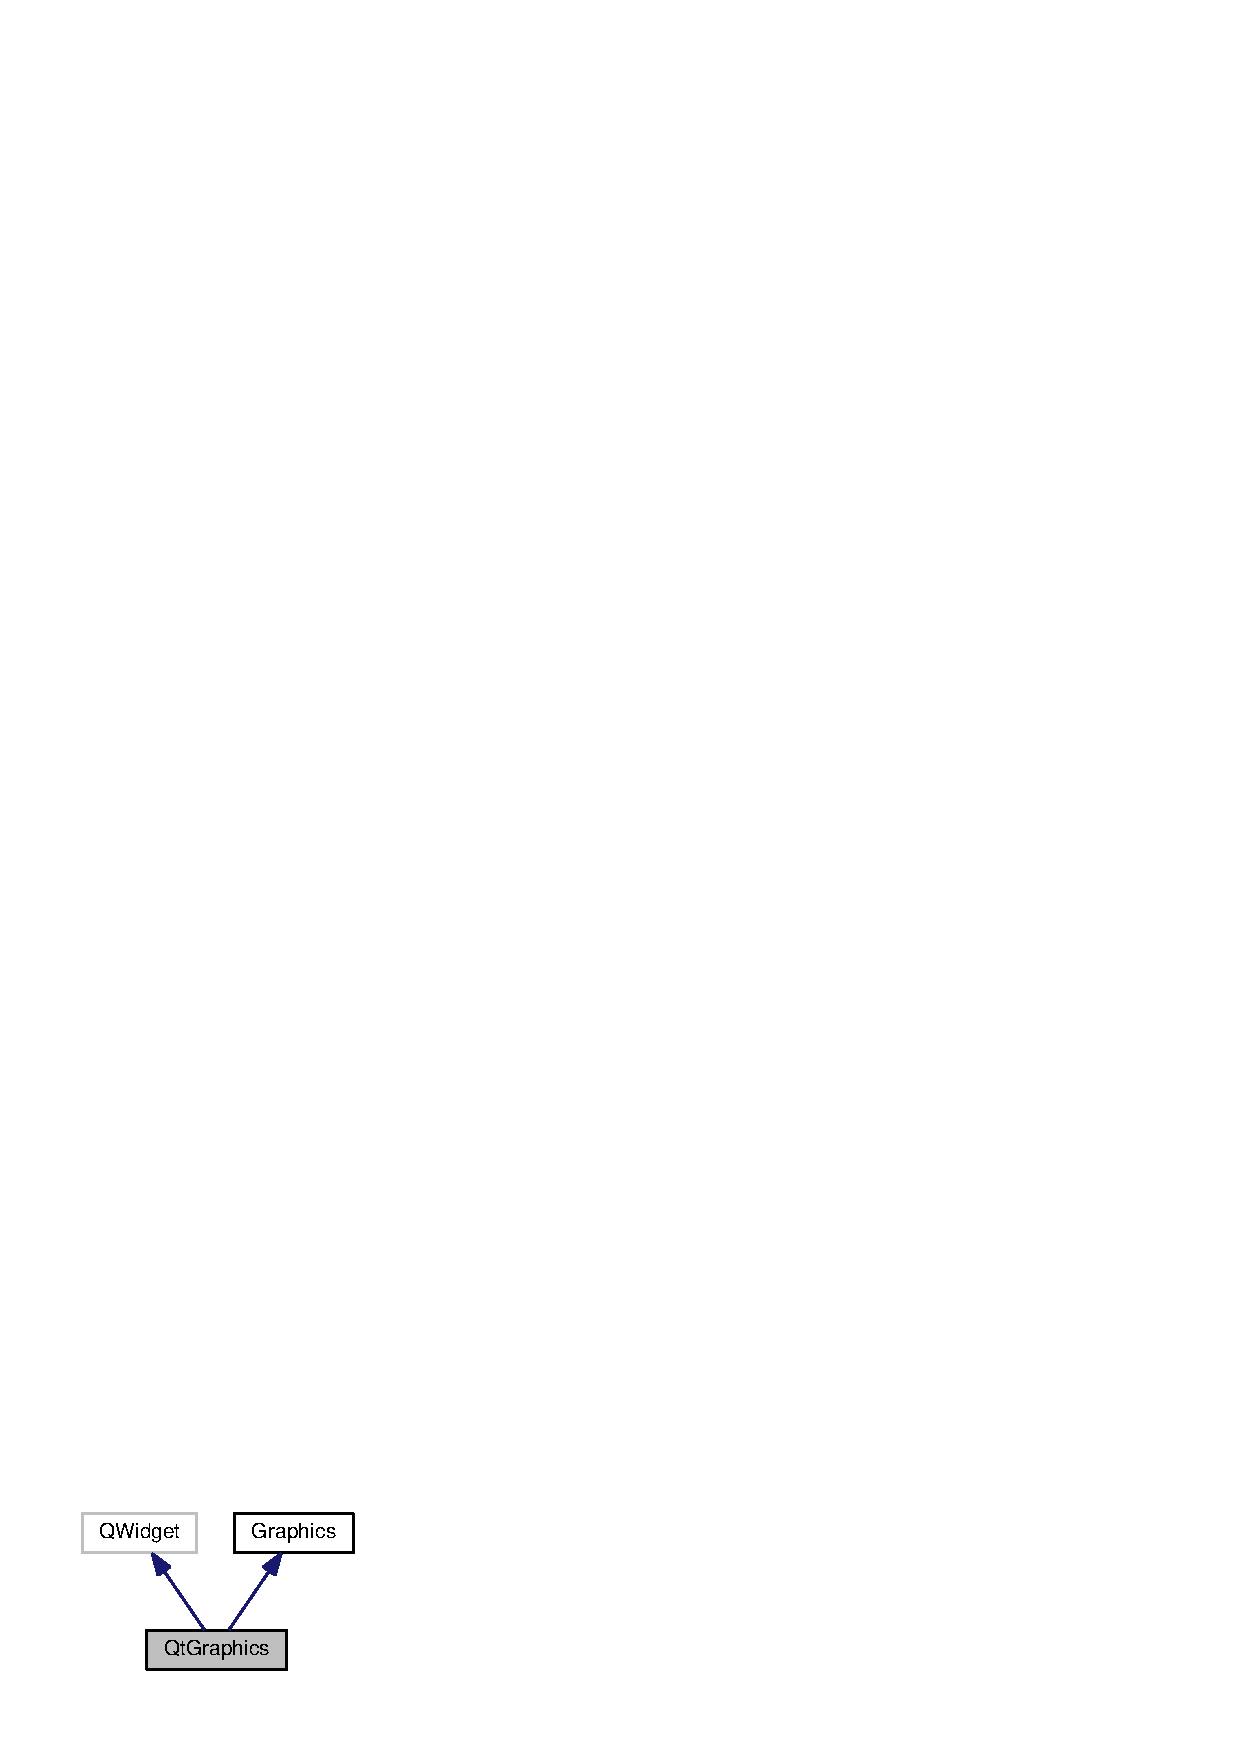
\includegraphics[width=173pt]{classQtGraphics__inherit__graph}
\end{center}
\end{figure}


Collaboration diagram for Qt\-Graphics\-:
\nopagebreak
\begin{figure}[H]
\begin{center}
\leavevmode
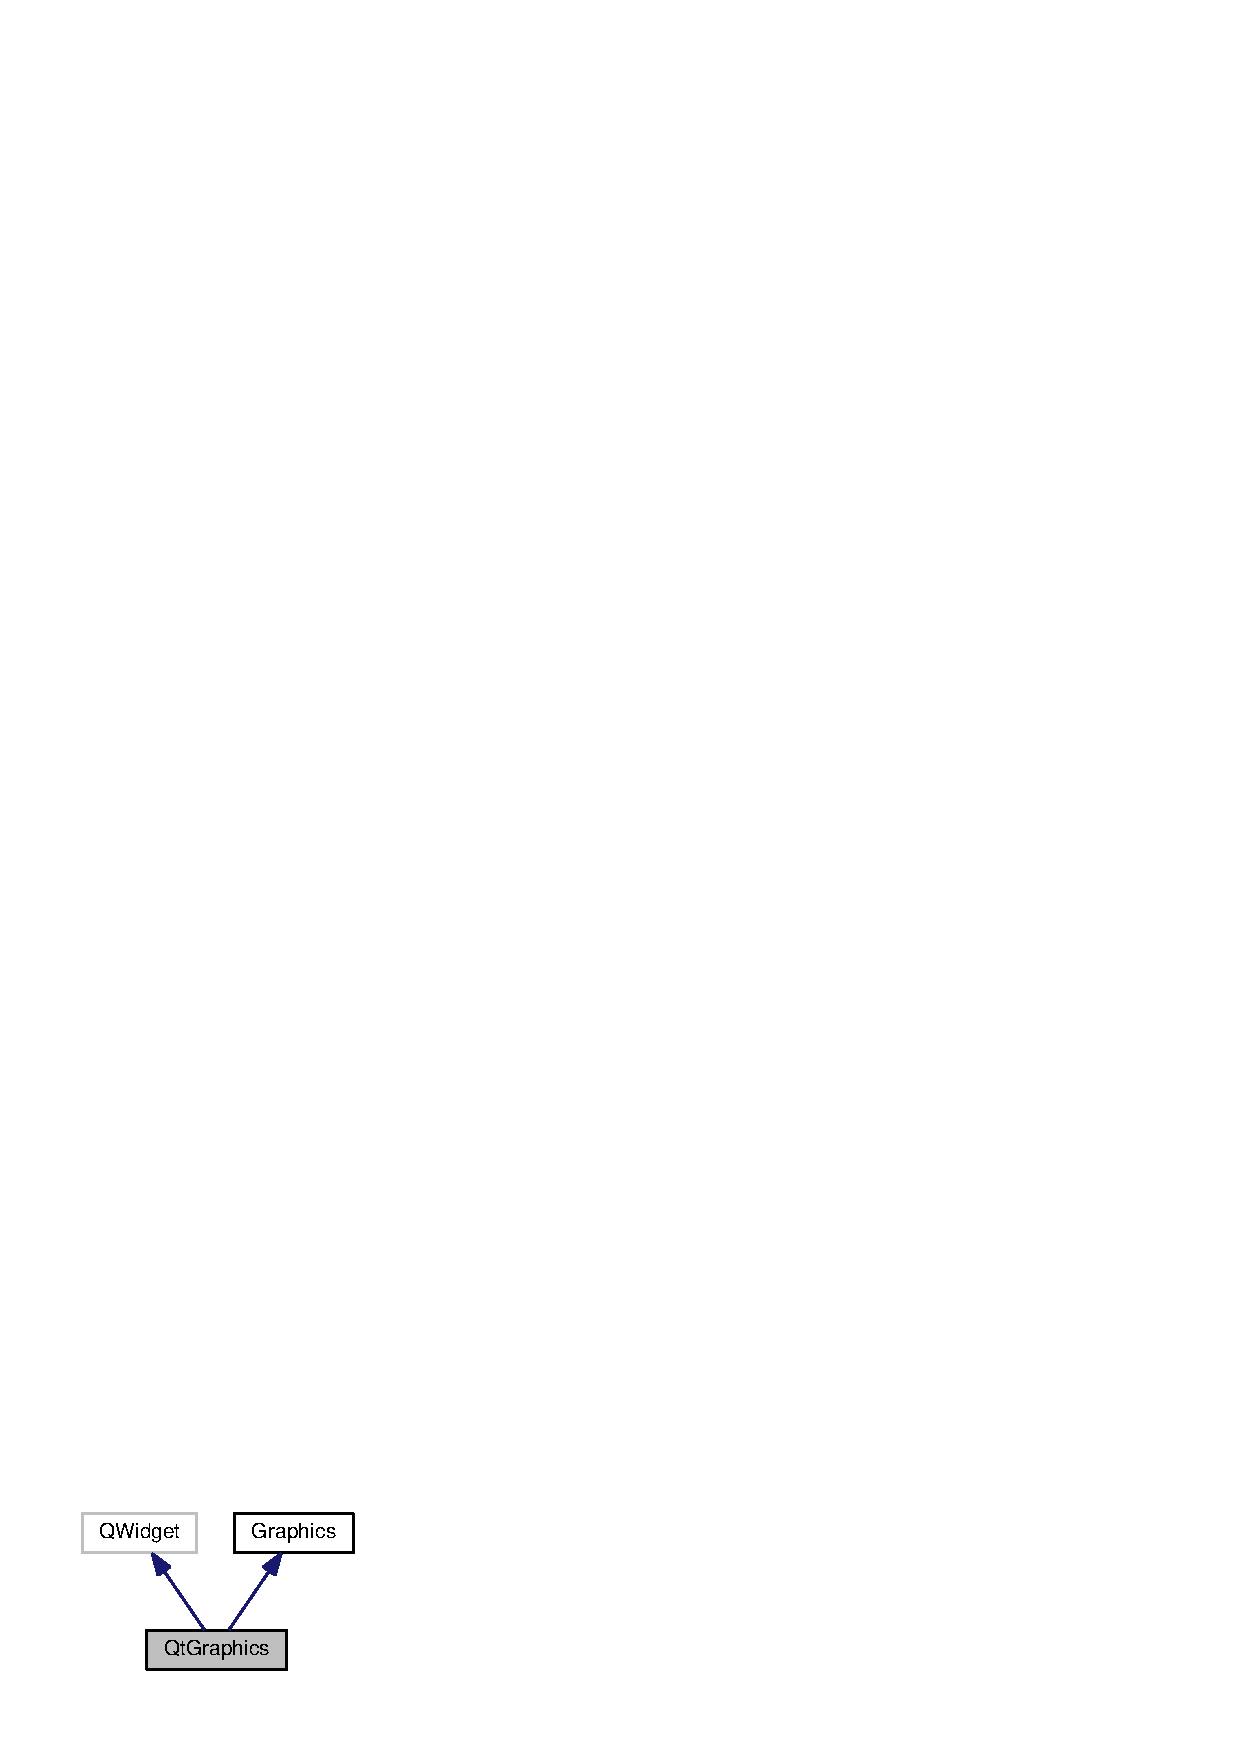
\includegraphics[width=173pt]{classQtGraphics__coll__graph}
\end{center}
\end{figure}
\subsection*{Public Slots}
\begin{DoxyCompactItemize}
\item 
void {\bf Time\-Step\-Wrap} (void)
\end{DoxyCompactItemize}
\subsection*{Signals}
\begin{DoxyCompactItemize}
\item 
void {\bf Simulation\-Done} (void)
\end{DoxyCompactItemize}
\subsection*{Public Member Functions}
\begin{DoxyCompactItemize}
\item 
{\bf Qt\-Graphics} (int xfield, int yfield, const char $\ast$movie\-\_\-file=0)
\item 
{\bf Qt\-Graphics} (Q\-Widget $\ast$parent, const char $\ast$name, int xfield, int yfield, const char $\ast$movie\-\_\-file=0)
\item 
virtual {\bf $\sim$\-Qt\-Graphics} (void)
\item 
virtual void {\bf Begin\-Scene} (void)
\begin{DoxyCompactList}\small\item\em \doxyref{Begin\-Scene()}{p.}{classQtGraphics_afd6200f3cbb931d811791f7683425f84} must be called before calling drawing functions. \end{DoxyCompactList}\item 
virtual void {\bf End\-Scene} (void)
\begin{DoxyCompactList}\small\item\em \doxyref{End\-Scene()}{p.}{classQtGraphics_a937c2227c5d121f56f9651d3aeccc27a} must be called to flush the drawing buffer and display the scene. \end{DoxyCompactList}\item 
virtual void {\bf Point} (int colour, int i, int j)
\begin{DoxyCompactList}\small\item\em Plot a point in the \doxyref{Graphics}{p.}{classGraphics} window. \end{DoxyCompactList}\item 
virtual void {\bf Line} (int x1, int y1, int x2, int y2, int colour)
\begin{DoxyCompactList}\small\item\em Draws a line (obviously... \-:-\/) \end{DoxyCompactList}\item 
virtual int {\bf Get\-X\-Y\-Coo} (int $\ast$X, int $\ast$Y)
\begin{DoxyCompactList}\small\item\em Probes the Window for user interaction, with mouse or keyboard. \end{DoxyCompactList}\item 
virtual int {\bf X\-Field} (void) const 
\begin{DoxyCompactList}\small\item\em Returns the width of the \doxyref{Graphics}{p.}{classGraphics} window, in pixels. \end{DoxyCompactList}\item 
virtual int {\bf Y\-Field} (void) const 
\begin{DoxyCompactList}\small\item\em Returns the height of the \doxyref{Graphics}{p.}{classGraphics} window, in pixels. \end{DoxyCompactList}\item 
virtual void {\bf Write} (char $\ast$fname, int quality=-\/1)
\begin{DoxyCompactList}\small\item\em Writes the Image to a file. \end{DoxyCompactList}\item 
void {\bf Clear\-Image} (void)
\item 
virtual void {\bf Time\-Step} (void)
\begin{DoxyCompactList}\small\item\em Implement this member function in your simulation code. \end{DoxyCompactList}\item 
virtual void {\bf resize\-Event} (Q\-Resize\-Event $\ast$event)
\end{DoxyCompactItemize}


\subsection{Constructor \& Destructor Documentation}
\index{Qt\-Graphics@{Qt\-Graphics}!Qt\-Graphics@{Qt\-Graphics}}
\index{Qt\-Graphics@{Qt\-Graphics}!QtGraphics@{Qt\-Graphics}}
\subsubsection[{Qt\-Graphics}]{\setlength{\rightskip}{0pt plus 5cm}Qt\-Graphics\-::\-Qt\-Graphics (
\begin{DoxyParamCaption}
\item[{int}]{xfield, }
\item[{int}]{yfield, }
\item[{const char $\ast$}]{movie\-\_\-file = {\ttfamily 0}}
\end{DoxyParamCaption}
)}\label{classQtGraphics_ac88e86da51667aca614769e96dd0a139}


Referenced by Qt\-Graphics().

\index{Qt\-Graphics@{Qt\-Graphics}!Qt\-Graphics@{Qt\-Graphics}}
\index{Qt\-Graphics@{Qt\-Graphics}!QtGraphics@{Qt\-Graphics}}
\subsubsection[{Qt\-Graphics}]{\setlength{\rightskip}{0pt plus 5cm}Qt\-Graphics\-::\-Qt\-Graphics (
\begin{DoxyParamCaption}
\item[{Q\-Widget $\ast$}]{parent, }
\item[{const char $\ast$}]{name, }
\item[{int}]{xfield, }
\item[{int}]{yfield, }
\item[{const char $\ast$}]{movie\-\_\-file = {\ttfamily 0}}
\end{DoxyParamCaption}
)\hspace{0.3cm}{\ttfamily [inline]}}\label{classQtGraphics_afc0891f050f33443d6b74ff3d23bd4a6}


References Qt\-Graphics().

\index{Qt\-Graphics@{Qt\-Graphics}!$\sim$\-Qt\-Graphics@{$\sim$\-Qt\-Graphics}}
\index{$\sim$\-Qt\-Graphics@{$\sim$\-Qt\-Graphics}!QtGraphics@{Qt\-Graphics}}
\subsubsection[{$\sim$\-Qt\-Graphics}]{\setlength{\rightskip}{0pt plus 5cm}Qt\-Graphics\-::$\sim$\-Qt\-Graphics (
\begin{DoxyParamCaption}
\item[{void}]{}
\end{DoxyParamCaption}
)\hspace{0.3cm}{\ttfamily [virtual]}}\label{classQtGraphics_ad223f63bd79cb211ac915a025bb04e91}


\subsection{Member Function Documentation}
\index{Qt\-Graphics@{Qt\-Graphics}!Begin\-Scene@{Begin\-Scene}}
\index{Begin\-Scene@{Begin\-Scene}!QtGraphics@{Qt\-Graphics}}
\subsubsection[{Begin\-Scene}]{\setlength{\rightskip}{0pt plus 5cm}void Qt\-Graphics\-::\-Begin\-Scene (
\begin{DoxyParamCaption}
\item[{void}]{}
\end{DoxyParamCaption}
)\hspace{0.3cm}{\ttfamily [virtual]}}\label{classQtGraphics_afd6200f3cbb931d811791f7683425f84}


\doxyref{Begin\-Scene()}{p.}{classQtGraphics_afd6200f3cbb931d811791f7683425f84} must be called before calling drawing functions. 



Reimplemented from {\bf Graphics} \doxyref{}{p.}{classGraphics_afc5b72e258d26775418c72c78d078e4b}.

\index{Qt\-Graphics@{Qt\-Graphics}!Clear\-Image@{Clear\-Image}}
\index{Clear\-Image@{Clear\-Image}!QtGraphics@{Qt\-Graphics}}
\subsubsection[{Clear\-Image}]{\setlength{\rightskip}{0pt plus 5cm}void Qt\-Graphics\-::\-Clear\-Image (
\begin{DoxyParamCaption}
\item[{void}]{}
\end{DoxyParamCaption}
)\hspace{0.3cm}{\ttfamily [inline]}}\label{classQtGraphics_acf960a2e8ccb605bb73dcd5694150a40}
\index{Qt\-Graphics@{Qt\-Graphics}!End\-Scene@{End\-Scene}}
\index{End\-Scene@{End\-Scene}!QtGraphics@{Qt\-Graphics}}
\subsubsection[{End\-Scene}]{\setlength{\rightskip}{0pt plus 5cm}void Qt\-Graphics\-::\-End\-Scene (
\begin{DoxyParamCaption}
\item[{void}]{}
\end{DoxyParamCaption}
)\hspace{0.3cm}{\ttfamily [virtual]}}\label{classQtGraphics_a937c2227c5d121f56f9651d3aeccc27a}


\doxyref{End\-Scene()}{p.}{classQtGraphics_a937c2227c5d121f56f9651d3aeccc27a} must be called to flush the drawing buffer and display the scene. 



Reimplemented from {\bf Graphics} \doxyref{}{p.}{classGraphics_a9f97b7c6506dcba845a1da457398fa90}.

\index{Qt\-Graphics@{Qt\-Graphics}!Get\-X\-Y\-Coo@{Get\-X\-Y\-Coo}}
\index{Get\-X\-Y\-Coo@{Get\-X\-Y\-Coo}!QtGraphics@{Qt\-Graphics}}
\subsubsection[{Get\-X\-Y\-Coo}]{\setlength{\rightskip}{0pt plus 5cm}int Qt\-Graphics\-::\-Get\-X\-Y\-Coo (
\begin{DoxyParamCaption}
\item[{int $\ast$}]{X, }
\item[{int $\ast$}]{Y}
\end{DoxyParamCaption}
)\hspace{0.3cm}{\ttfamily [virtual]}}\label{classQtGraphics_a497ca587ebbac0336589066147de3ab5}


Probes the Window for user interaction, with mouse or keyboard. 

This function should return immediately, and return 0 if there was no user interaction.


\begin{DoxyParams}{Parameters}
{\em $\ast$\-X,$\ast$\-Y} & Pointer where the clicked coordinate will be stored. \\
\hline
\end{DoxyParams}


Implements {\bf Graphics} \doxyref{}{p.}{classGraphics_a39257f929b38739ed42e8d463c4f42c3}.

\index{Qt\-Graphics@{Qt\-Graphics}!Line@{Line}}
\index{Line@{Line}!QtGraphics@{Qt\-Graphics}}
\subsubsection[{Line}]{\setlength{\rightskip}{0pt plus 5cm}void Qt\-Graphics\-::\-Line (
\begin{DoxyParamCaption}
\item[{int}]{x1, }
\item[{int}]{y1, }
\item[{int}]{x2, }
\item[{int}]{y2, }
\item[{int}]{colour}
\end{DoxyParamCaption}
)\hspace{0.3cm}{\ttfamily [virtual]}}\label{classQtGraphics_a4ca1bd37d041d0741fd4c82e0705511b}


Draws a line (obviously... \-:-\/) 


\begin{DoxyParams}{Parameters}
{\em x1,y1} & First coordinate pair. \\
\hline
{\em x2,y2} & Second coordinate pair. \\
\hline
{\em color} & Color of the line, as given in the colormap file \char`\"{}default.\-ctb\char`\"{}. \\
\hline
\end{DoxyParams}


Implements {\bf Graphics} \doxyref{}{p.}{classGraphics_a8e049566ac4cf6168b04f0f8be7a9820}.

\index{Qt\-Graphics@{Qt\-Graphics}!Point@{Point}}
\index{Point@{Point}!QtGraphics@{Qt\-Graphics}}
\subsubsection[{Point}]{\setlength{\rightskip}{0pt plus 5cm}void Qt\-Graphics\-::\-Point (
\begin{DoxyParamCaption}
\item[{int}]{color, }
\item[{int}]{x, }
\item[{int}]{y}
\end{DoxyParamCaption}
)\hspace{0.3cm}{\ttfamily [virtual]}}\label{classQtGraphics_ad02ff8ba69d13148f79afd516563b822}


Plot a point in the \doxyref{Graphics}{p.}{classGraphics} window. 


\begin{DoxyParams}{Parameters}
{\em color} & Color index, as defined in colormap file \char`\"{}default.\-ctb\char`\"{}, which should be in the same directory as the executable. \\
\hline
{\em x,y} & Coordinate of point, in \doxyref{Graphics}{p.}{classGraphics} coordinates (typically twice as large as the cellular automata coordinates). \\
\hline
\end{DoxyParams}


Implements {\bf Graphics} \doxyref{}{p.}{classGraphics_a123e1b2c757c39bf329517af332c24eb}.

\index{Qt\-Graphics@{Qt\-Graphics}!resize\-Event@{resize\-Event}}
\index{resize\-Event@{resize\-Event}!QtGraphics@{Qt\-Graphics}}
\subsubsection[{resize\-Event}]{\setlength{\rightskip}{0pt plus 5cm}void Qt\-Graphics\-::resize\-Event (
\begin{DoxyParamCaption}
\item[{Q\-Resize\-Event $\ast$}]{event}
\end{DoxyParamCaption}
)\hspace{0.3cm}{\ttfamily [virtual]}}\label{classQtGraphics_ae8bbdebe79908f7d0d728407438edcef}
\index{Qt\-Graphics@{Qt\-Graphics}!Simulation\-Done@{Simulation\-Done}}
\index{Simulation\-Done@{Simulation\-Done}!QtGraphics@{Qt\-Graphics}}
\subsubsection[{Simulation\-Done}]{\setlength{\rightskip}{0pt plus 5cm}void Qt\-Graphics\-::\-Simulation\-Done (
\begin{DoxyParamCaption}
\item[{void}]{}
\end{DoxyParamCaption}
)\hspace{0.3cm}{\ttfamily [signal]}}\label{classQtGraphics_ad3a71c2118a9f6156bd12a953c1f7788}
\index{Qt\-Graphics@{Qt\-Graphics}!Time\-Step@{Time\-Step}}
\index{Time\-Step@{Time\-Step}!QtGraphics@{Qt\-Graphics}}
\subsubsection[{Time\-Step}]{\setlength{\rightskip}{0pt plus 5cm}virtual void Qt\-Graphics\-::\-Time\-Step (
\begin{DoxyParamCaption}
\item[{void}]{}
\end{DoxyParamCaption}
)\hspace{0.3cm}{\ttfamily [virtual]}}\label{classQtGraphics_a6c3e54b681404b550417628910557ade}


Implement this member function in your simulation code. 

Include all actions that should be carried out during a simulation step, including \doxyref{P\-D\-E}{p.}{classPDE} and C\-P\-M simulation steps. See the included examples (\doxyref{vessel.\-cpp}{p.}{vessel_8cpp}, \doxyref{sorting.\-cpp}{p.}{sorting_8cpp}) for more information. 

Reimplemented from {\bf Graphics} \doxyref{}{p.}{classGraphics_aa1b61fa6f6bc50aceff6f320ce5b9be2}.

\index{Qt\-Graphics@{Qt\-Graphics}!Time\-Step\-Wrap@{Time\-Step\-Wrap}}
\index{Time\-Step\-Wrap@{Time\-Step\-Wrap}!QtGraphics@{Qt\-Graphics}}
\subsubsection[{Time\-Step\-Wrap}]{\setlength{\rightskip}{0pt plus 5cm}void Qt\-Graphics\-::\-Time\-Step\-Wrap (
\begin{DoxyParamCaption}
\item[{void}]{}
\end{DoxyParamCaption}
)\hspace{0.3cm}{\ttfamily [slot]}}\label{classQtGraphics_ab6ef76ce60c71c106e36c329c6d3b594}


References Parameter\-::mcs, and par.

\index{Qt\-Graphics@{Qt\-Graphics}!Write@{Write}}
\index{Write@{Write}!QtGraphics@{Qt\-Graphics}}
\subsubsection[{Write}]{\setlength{\rightskip}{0pt plus 5cm}void Qt\-Graphics\-::\-Write (
\begin{DoxyParamCaption}
\item[{char $\ast$}]{fname, }
\item[{int}]{quality = {\ttfamily -\/1}}
\end{DoxyParamCaption}
)\hspace{0.3cm}{\ttfamily [virtual]}}\label{classQtGraphics_a2b3ae718854987c2746f8d723fbf3fa6}


Writes the Image to a file. 

File format is inferred from file extension. Currently only P\-N\-G is supported by the X-\/\-Windows implementation; the Qt-\/implentation supports all formats supported by Qt.


\begin{DoxyParams}{Parameters}
{\em fname} & File name with standard image file extension (e.\-g. png). \\
\hline
{\em quality} & Quality of J\-P\-E\-G images, defaults to -\/1 (no value provided). \\
\hline
\end{DoxyParams}


Implements {\bf Graphics} \doxyref{}{p.}{classGraphics_af98a333b8be25817669e615b1cd6c73d}.

\index{Qt\-Graphics@{Qt\-Graphics}!X\-Field@{X\-Field}}
\index{X\-Field@{X\-Field}!QtGraphics@{Qt\-Graphics}}
\subsubsection[{X\-Field}]{\setlength{\rightskip}{0pt plus 5cm}virtual int Qt\-Graphics\-::\-X\-Field (
\begin{DoxyParamCaption}
\item[{void}]{}
\end{DoxyParamCaption}
) const\hspace{0.3cm}{\ttfamily [inline]}, {\ttfamily [virtual]}}\label{classQtGraphics_ae18cae9c5ade06e287f40190b919639d}


Returns the width of the \doxyref{Graphics}{p.}{classGraphics} window, in pixels. 



Reimplemented from {\bf Graphics} \doxyref{}{p.}{classGraphics_a57a2d92f0744fe35be0a712803178a4f}.

\index{Qt\-Graphics@{Qt\-Graphics}!Y\-Field@{Y\-Field}}
\index{Y\-Field@{Y\-Field}!QtGraphics@{Qt\-Graphics}}
\subsubsection[{Y\-Field}]{\setlength{\rightskip}{0pt plus 5cm}virtual int Qt\-Graphics\-::\-Y\-Field (
\begin{DoxyParamCaption}
\item[{void}]{}
\end{DoxyParamCaption}
) const\hspace{0.3cm}{\ttfamily [inline]}, {\ttfamily [virtual]}}\label{classQtGraphics_a9945f6ee5fa3ddf649a5a4ac52785356}


Returns the height of the \doxyref{Graphics}{p.}{classGraphics} window, in pixels. 



Reimplemented from {\bf Graphics} \doxyref{}{p.}{classGraphics_ad9df13b4bb136c8c5ca802ec8f382e47}.



The documentation for this class was generated from the following files\-:\begin{DoxyCompactItemize}
\item 
{\bf qtgraph.\-h}\item 
{\bf qt3graph.\-cpp}\item 
{\bf qtgraph.\-cpp}\end{DoxyCompactItemize}

\section{X11\-Graphics Class Reference}
\label{classX11Graphics}\index{X11\-Graphics@{X11\-Graphics}}


X-\/\-Windows implementation of \doxyref{Graphics}{p.}{classGraphics} interface.  




{\ttfamily \#include $<$x11graph.\-h$>$}



Inheritance diagram for X11\-Graphics\-:
\nopagebreak
\begin{figure}[H]
\begin{center}
\leavevmode
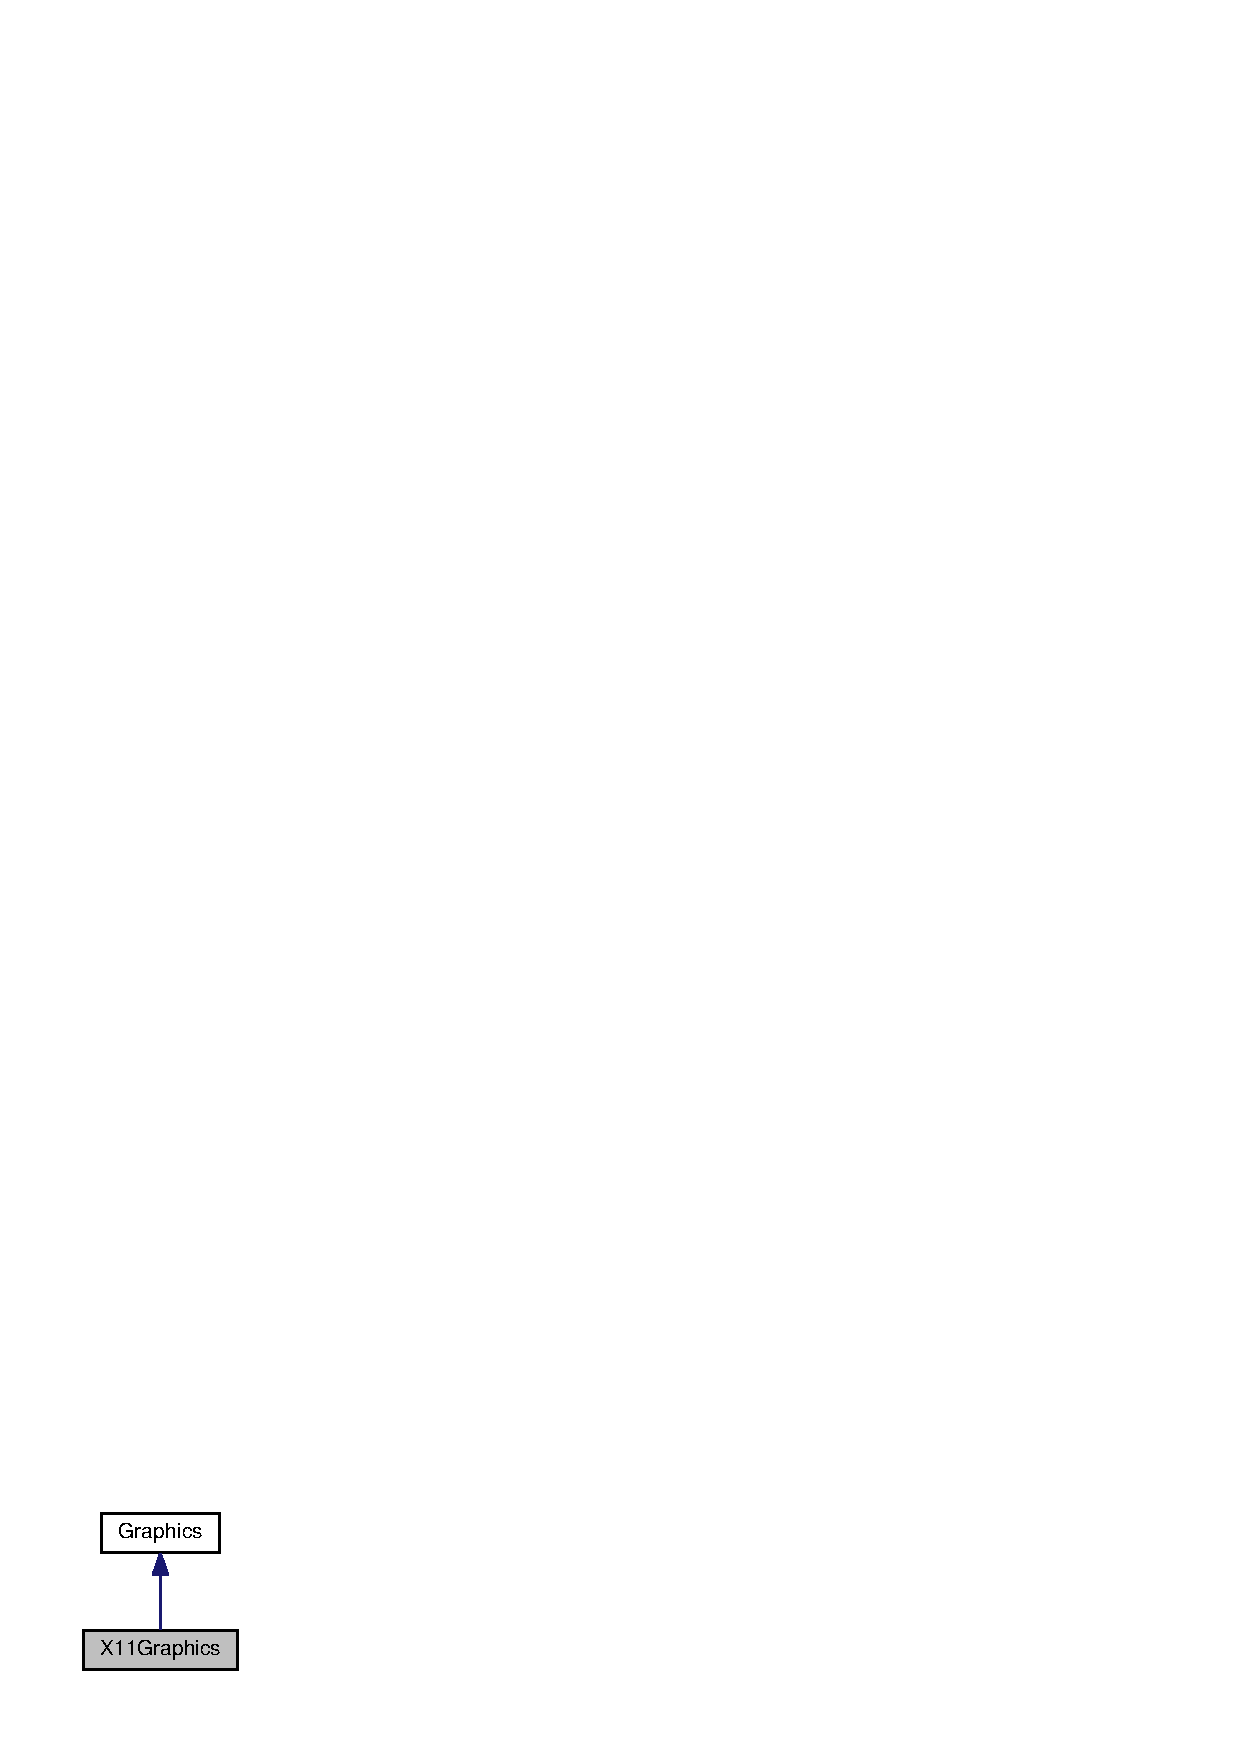
\includegraphics[width=118pt]{classX11Graphics__inherit__graph}
\end{center}
\end{figure}


Collaboration diagram for X11\-Graphics\-:
\nopagebreak
\begin{figure}[H]
\begin{center}
\leavevmode
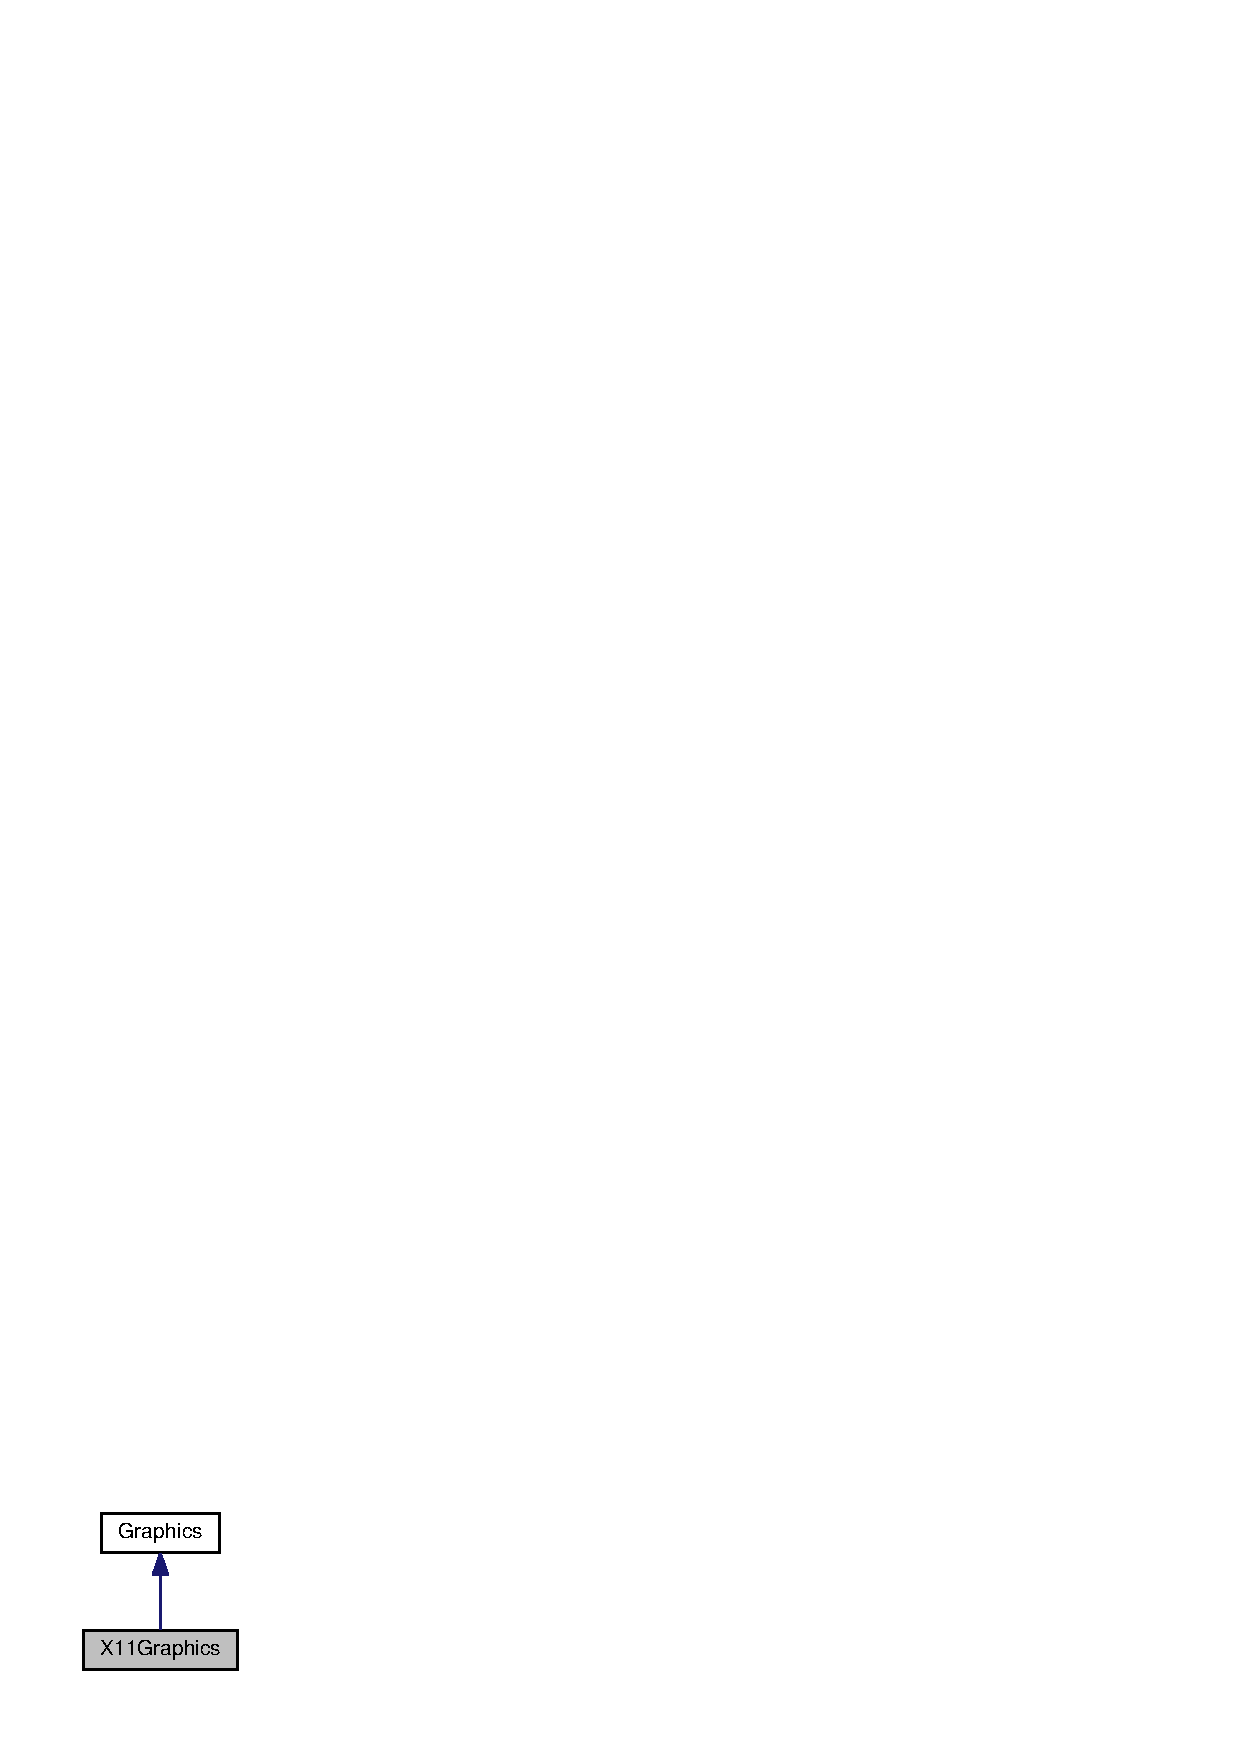
\includegraphics[width=118pt]{classX11Graphics__coll__graph}
\end{center}
\end{figure}
\subsection*{Public Member Functions}
\begin{DoxyCompactItemize}
\item 
{\bf X11\-Graphics} (int xfield, int yfield, const char $\ast$movie\-\_\-file=0)
\item 
virtual {\bf $\sim$\-X11\-Graphics} (void)
\item 
virtual void {\bf Begin\-Scene} (void)
\begin{DoxyCompactList}\small\item\em \doxyref{Begin\-Scene()}{p.}{classX11Graphics_af90168e2537eb714dd0d916a2c543f74} must be called before calling drawing functions. \end{DoxyCompactList}\item 
virtual void {\bf End\-Scene} (void)
\begin{DoxyCompactList}\small\item\em \doxyref{End\-Scene()}{p.}{classX11Graphics_aeafb2bf394ef9dfd3aa9b390d2b21d7a} must be called to flush the drawing buffer and display the scene. \end{DoxyCompactList}\item 
void {\bf Flush} (void)
\begin{DoxyCompactList}\small\item\em Flushes scene to window. Normally called by \doxyref{End\-Scene()}{p.}{classX11Graphics_aeafb2bf394ef9dfd3aa9b390d2b21d7a}. \end{DoxyCompactList}\item 
virtual void {\bf Point} (int color, int x, int y)
\begin{DoxyCompactList}\small\item\em Plot a point in the \doxyref{Graphics}{p.}{classGraphics} window. \end{DoxyCompactList}\item 
virtual void {\bf Line} (int x1, int y1, int x2, int y2, int colour)
\begin{DoxyCompactList}\small\item\em Draws a line (obviously... \-:-\/) \end{DoxyCompactList}\item 
void {\bf Field} (const int $\ast$$\ast$r, int mag=1)
\begin{DoxyCompactList}\small\item\em Plots a field of values given by $\ast$$\ast$f, using color coding given by colormap file. \end{DoxyCompactList}\item 
virtual int {\bf Get\-X\-Y\-Coo} (int $\ast$X, int $\ast$Y)
\begin{DoxyCompactList}\small\item\em Probes the Window for user interaction, with mouse or keyboard. \end{DoxyCompactList}\item 
char $\ast$ {\bf Change\-Title} (const char $\ast$message)
\begin{DoxyCompactList}\small\item\em Changes the title bar of the \doxyref{Graphics}{p.}{classGraphics} window. \end{DoxyCompactList}\item 
void {\bf Recover\-Title} (void)
\begin{DoxyCompactList}\small\item\em Recovers the title prior to the last call of \doxyref{Change\-Title()}{p.}{classX11Graphics_adcce6fa1eab8d9a059333e9b1cc8580e}. \end{DoxyCompactList}\item 
{\bf Line\-Type} {\bf Crop\-Size} (void)
\begin{DoxyCompactList}\small\item\em Returns the upper left and lower right coordinates of the area occupied by cells. \end{DoxyCompactList}\item 
{\bf Coordinate} {\bf Replace\-Beast} ({\bf Coordinate} old\-\_\-size, {\bf Coordinate} new\-\_\-size)
\begin{DoxyCompactList}\small\item\em This member function was part of functionality that enables interactive resizing of the Window and C\-P\-M field, and followed by interactive replacement of the \doxyref{Dish}{p.}{classDish}'s contents. The current version of C\-P\-M does not contain such functionality. \end{DoxyCompactList}\item 
virtual int {\bf X\-Field} (void) const 
\begin{DoxyCompactList}\small\item\em Returns the width of the \doxyref{Graphics}{p.}{classGraphics} window, in pixels. \end{DoxyCompactList}\item 
virtual int {\bf Y\-Field} (void) const 
\begin{DoxyCompactList}\small\item\em Returns the height of the \doxyref{Graphics}{p.}{classGraphics} window, in pixels. \end{DoxyCompactList}\item 
virtual void {\bf Write} (char $\ast$fname, int quality=-\/1)
\begin{DoxyCompactList}\small\item\em Writes the Image to a file. \end{DoxyCompactList}\item 
void {\bf Clear\-Image} (void)
\begin{DoxyCompactList}\small\item\em Clears all pixels in the Image. \end{DoxyCompactList}\item 
virtual void {\bf Time\-Step} (void)
\begin{DoxyCompactList}\small\item\em Implement this member function in your simulation code. \end{DoxyCompactList}\end{DoxyCompactItemize}


\subsection{Detailed Description}
X-\/\-Windows implementation of \doxyref{Graphics}{p.}{classGraphics} interface. 

For A\-P\-I see documentation of base class \doxyref{Graphics}{p.}{classGraphics}.

Has a number extra features\-: see below. 

\subsection{Constructor \& Destructor Documentation}
\index{X11\-Graphics@{X11\-Graphics}!X11\-Graphics@{X11\-Graphics}}
\index{X11\-Graphics@{X11\-Graphics}!X11Graphics@{X11\-Graphics}}
\subsubsection[{X11\-Graphics}]{\setlength{\rightskip}{0pt plus 5cm}X11\-Graphics\-::\-X11\-Graphics (
\begin{DoxyParamCaption}
\item[{int}]{xfield, }
\item[{int}]{yfield, }
\item[{const char $\ast$}]{movie\-\_\-file = {\ttfamily 0}}
\end{DoxyParamCaption}
)}\label{classX11Graphics_a3aacea46496509c62c7d5c351dd9ddae}


References Parameter\-::graphics, and Parameter\-::store.

\index{X11\-Graphics@{X11\-Graphics}!$\sim$\-X11\-Graphics@{$\sim$\-X11\-Graphics}}
\index{$\sim$\-X11\-Graphics@{$\sim$\-X11\-Graphics}!X11Graphics@{X11\-Graphics}}
\subsubsection[{$\sim$\-X11\-Graphics}]{\setlength{\rightskip}{0pt plus 5cm}X11\-Graphics\-::$\sim$\-X11\-Graphics (
\begin{DoxyParamCaption}
\item[{void}]{}
\end{DoxyParamCaption}
)\hspace{0.3cm}{\ttfamily [virtual]}}\label{classX11Graphics_a8231cf37901518bda06b8b6c3aafb8cf}


\subsection{Member Function Documentation}
\index{X11\-Graphics@{X11\-Graphics}!Begin\-Scene@{Begin\-Scene}}
\index{Begin\-Scene@{Begin\-Scene}!X11Graphics@{X11\-Graphics}}
\subsubsection[{Begin\-Scene}]{\setlength{\rightskip}{0pt plus 5cm}void X11\-Graphics\-::\-Begin\-Scene (
\begin{DoxyParamCaption}
\item[{void}]{}
\end{DoxyParamCaption}
)\hspace{0.3cm}{\ttfamily [virtual]}}\label{classX11Graphics_af90168e2537eb714dd0d916a2c543f74}


\doxyref{Begin\-Scene()}{p.}{classX11Graphics_af90168e2537eb714dd0d916a2c543f74} must be called before calling drawing functions. 



Reimplemented from {\bf Graphics} \doxyref{}{p.}{classGraphics_afc5b72e258d26775418c72c78d078e4b}.

\index{X11\-Graphics@{X11\-Graphics}!Change\-Title@{Change\-Title}}
\index{Change\-Title@{Change\-Title}!X11Graphics@{X11\-Graphics}}
\subsubsection[{Change\-Title}]{\setlength{\rightskip}{0pt plus 5cm}char $\ast$ X11\-Graphics\-::\-Change\-Title (
\begin{DoxyParamCaption}
\item[{const char $\ast$}]{message}
\end{DoxyParamCaption}
)}\label{classX11Graphics_adcce6fa1eab8d9a059333e9b1cc8580e}


Changes the title bar of the \doxyref{Graphics}{p.}{classGraphics} window. 


\begin{DoxyParams}{Parameters}
{\em message} & Text to display in title bar. \\
\hline
\end{DoxyParams}


Referenced by Recover\-Title(), and Replace\-Beast().

\index{X11\-Graphics@{X11\-Graphics}!Clear\-Image@{Clear\-Image}}
\index{Clear\-Image@{Clear\-Image}!X11Graphics@{X11\-Graphics}}
\subsubsection[{Clear\-Image}]{\setlength{\rightskip}{0pt plus 5cm}void X11\-Graphics\-::\-Clear\-Image (
\begin{DoxyParamCaption}
\item[{void}]{}
\end{DoxyParamCaption}
)\hspace{0.3cm}{\ttfamily [inline]}}\label{classX11Graphics_a5191f505f8bc85fbe8c33992fa9fe4f1}


Clears all pixels in the Image. 



References Point().

\index{X11\-Graphics@{X11\-Graphics}!Crop\-Size@{Crop\-Size}}
\index{Crop\-Size@{Crop\-Size}!X11Graphics@{X11\-Graphics}}
\subsubsection[{Crop\-Size}]{\setlength{\rightskip}{0pt plus 5cm}{\bf Line\-Type} X11\-Graphics\-::\-Crop\-Size (
\begin{DoxyParamCaption}
\item[{void}]{}
\end{DoxyParamCaption}
)}\label{classX11Graphics_a71f50f8405a9ceae42e4035ab7d41451}


Returns the upper left and lower right coordinates of the area occupied by cells. 

\begin{DoxyReturn}{Returns}
Bounding box as a Line\-Type structure \{int x1,int y1,int x2,int y2\}.
\end{DoxyReturn}
Warning\-: Assumes the window only displays cells (i.\-e. no \doxyref{P\-D\-E}{p.}{classPDE} fields etc.). If you need this, better implement it as a member function of class \doxyref{Cellular\-Potts}{p.}{classCellularPotts}. 

References li\-::x1, li\-::x2, li\-::y1, and li\-::y2.

\index{X11\-Graphics@{X11\-Graphics}!End\-Scene@{End\-Scene}}
\index{End\-Scene@{End\-Scene}!X11Graphics@{X11\-Graphics}}
\subsubsection[{End\-Scene}]{\setlength{\rightskip}{0pt plus 5cm}void X11\-Graphics\-::\-End\-Scene (
\begin{DoxyParamCaption}
\item[{void}]{}
\end{DoxyParamCaption}
)\hspace{0.3cm}{\ttfamily [virtual]}}\label{classX11Graphics_aeafb2bf394ef9dfd3aa9b390d2b21d7a}


\doxyref{End\-Scene()}{p.}{classX11Graphics_aeafb2bf394ef9dfd3aa9b390d2b21d7a} must be called to flush the drawing buffer and display the scene. 



Reimplemented from {\bf Graphics} \doxyref{}{p.}{classGraphics_a9f97b7c6506dcba845a1da457398fa90}.



References Parameter\-::graphics, and Parameter\-::storage\-\_\-stride.



Referenced by Field(), and Get\-X\-Y\-Coo().

\index{X11\-Graphics@{X11\-Graphics}!Field@{Field}}
\index{Field@{Field}!X11Graphics@{X11\-Graphics}}
\subsubsection[{Field}]{\setlength{\rightskip}{0pt plus 5cm}void X11\-Graphics\-::\-Field (
\begin{DoxyParamCaption}
\item[{const int $\ast$$\ast$}]{f, }
\item[{int}]{mag = {\ttfamily 1}}
\end{DoxyParamCaption}
)\hspace{0.3cm}{\ttfamily [virtual]}}\label{classX11Graphics_a4ba01ab14685f860af345b4ac17f3339}


Plots a field of values given by $\ast$$\ast$f, using color coding given by colormap file. 

Only implemented in \doxyref{X11\-Graphics}{p.}{classX11Graphics}. No checks. Usage not recommended.


\begin{DoxyParams}{Parameters}
{\em f} & Double pointer to array of integers, giving color indices using standard colormap ('default.\-ctb'). \\
\hline
{\em mag} & magnification factor. \\
\hline
\end{DoxyParams}


Reimplemented from {\bf Graphics} \doxyref{}{p.}{classGraphics_a22105e059337daabadfa68838811099f}.



References End\-Scene(), Parameter\-::graphics, and Point().

\index{X11\-Graphics@{X11\-Graphics}!Flush@{Flush}}
\index{Flush@{Flush}!X11Graphics@{X11\-Graphics}}
\subsubsection[{Flush}]{\setlength{\rightskip}{0pt plus 5cm}void X11\-Graphics\-::\-Flush (
\begin{DoxyParamCaption}
\item[{void}]{}
\end{DoxyParamCaption}
)\hspace{0.3cm}{\ttfamily [inline]}}\label{classX11Graphics_af7dc9389d25610c90f8da7f33bf42ecb}


Flushes scene to window. Normally called by \doxyref{End\-Scene()}{p.}{classX11Graphics_aeafb2bf394ef9dfd3aa9b390d2b21d7a}. 

\index{X11\-Graphics@{X11\-Graphics}!Get\-X\-Y\-Coo@{Get\-X\-Y\-Coo}}
\index{Get\-X\-Y\-Coo@{Get\-X\-Y\-Coo}!X11Graphics@{X11\-Graphics}}
\subsubsection[{Get\-X\-Y\-Coo}]{\setlength{\rightskip}{0pt plus 5cm}int X11\-Graphics\-::\-Get\-X\-Y\-Coo (
\begin{DoxyParamCaption}
\item[{int $\ast$}]{X, }
\item[{int $\ast$}]{Y}
\end{DoxyParamCaption}
)\hspace{0.3cm}{\ttfamily [virtual]}}\label{classX11Graphics_a2d3f6a3d4b3f0131dbfb9253d51f0ebc}


Probes the Window for user interaction, with mouse or keyboard. 

This function should return immediately, and return 0 if there was no user interaction.


\begin{DoxyParams}{Parameters}
{\em $\ast$\-X,$\ast$\-Y} & Pointer where the clicked coordinate will be stored. \\
\hline
\end{DoxyParams}


Implements {\bf Graphics} \doxyref{}{p.}{classGraphics_a39257f929b38739ed42e8d463c4f42c3}.



References End\-Scene(), Parameter\-::graphics, K\-E\-Y\-B\-U\-F\-S\-I\-Z\-E, M\-O\-T\-I\-O\-N, and R\-E\-S\-I\-Z\-E.



Referenced by Replace\-Beast().

\index{X11\-Graphics@{X11\-Graphics}!Line@{Line}}
\index{Line@{Line}!X11Graphics@{X11\-Graphics}}
\subsubsection[{Line}]{\setlength{\rightskip}{0pt plus 5cm}void X11\-Graphics\-::\-Line (
\begin{DoxyParamCaption}
\item[{int}]{x1, }
\item[{int}]{y1, }
\item[{int}]{x2, }
\item[{int}]{y2, }
\item[{int}]{colour}
\end{DoxyParamCaption}
)\hspace{0.3cm}{\ttfamily [virtual]}}\label{classX11Graphics_a8126d246d7925babf273df1fa948466d}


Draws a line (obviously... \-:-\/) 


\begin{DoxyParams}{Parameters}
{\em x1,y1} & First coordinate pair. \\
\hline
{\em x2,y2} & Second coordinate pair. \\
\hline
{\em color} & Color of the line, as given in the colormap file \char`\"{}default.\-ctb\char`\"{}. \\
\hline
\end{DoxyParams}


Implements {\bf Graphics} \doxyref{}{p.}{classGraphics_a8e049566ac4cf6168b04f0f8be7a9820}.



References Point(), and S\-W\-A\-P.

\index{X11\-Graphics@{X11\-Graphics}!Point@{Point}}
\index{Point@{Point}!X11Graphics@{X11\-Graphics}}
\subsubsection[{Point}]{\setlength{\rightskip}{0pt plus 5cm}void X11\-Graphics\-::\-Point (
\begin{DoxyParamCaption}
\item[{int}]{color, }
\item[{int}]{x, }
\item[{int}]{y}
\end{DoxyParamCaption}
)\hspace{0.3cm}{\ttfamily [virtual]}}\label{classX11Graphics_aac47663836332028e6a382af6a2c622c}


Plot a point in the \doxyref{Graphics}{p.}{classGraphics} window. 


\begin{DoxyParams}{Parameters}
{\em color} & Color index, as defined in colormap file \char`\"{}default.\-ctb\char`\"{}, which should be in the same directory as the executable. \\
\hline
{\em x,y} & Coordinate of point, in \doxyref{Graphics}{p.}{classGraphics} coordinates (typically twice as large as the cellular automata coordinates). \\
\hline
\end{DoxyParams}


Implements {\bf Graphics} \doxyref{}{p.}{classGraphics_a123e1b2c757c39bf329517af332c24eb}.



References Parameter\-::graphics.



Referenced by Clear\-Image(), Field(), and Line().

\index{X11\-Graphics@{X11\-Graphics}!Recover\-Title@{Recover\-Title}}
\index{Recover\-Title@{Recover\-Title}!X11Graphics@{X11\-Graphics}}
\subsubsection[{Recover\-Title}]{\setlength{\rightskip}{0pt plus 5cm}void X11\-Graphics\-::\-Recover\-Title (
\begin{DoxyParamCaption}
\item[{void}]{}
\end{DoxyParamCaption}
)}\label{classX11Graphics_a6b8fc3f7590a2f9ae5be1a3917b28cce}


Recovers the title prior to the last call of \doxyref{Change\-Title()}{p.}{classX11Graphics_adcce6fa1eab8d9a059333e9b1cc8580e}. 



References Change\-Title().



Referenced by Replace\-Beast().

\index{X11\-Graphics@{X11\-Graphics}!Replace\-Beast@{Replace\-Beast}}
\index{Replace\-Beast@{Replace\-Beast}!X11Graphics@{X11\-Graphics}}
\subsubsection[{Replace\-Beast}]{\setlength{\rightskip}{0pt plus 5cm}{\bf Coordinate} X11\-Graphics\-::\-Replace\-Beast (
\begin{DoxyParamCaption}
\item[{{\bf Coordinate}}]{old\-\_\-size, }
\item[{{\bf Coordinate}}]{new\-\_\-size}
\end{DoxyParamCaption}
)}\label{classX11Graphics_a934f355d684c9cb35542a6e63ff859be}


This member function was part of functionality that enables interactive resizing of the Window and C\-P\-M field, and followed by interactive replacement of the \doxyref{Dish}{p.}{classDish}'s contents. The current version of C\-P\-M does not contain such functionality. 



References Change\-Title(), Get\-X\-Y\-Coo(), M\-O\-T\-I\-O\-N, Recover\-Title(), T\-R\-U\-E, co\-::x, and co\-::y.

\index{X11\-Graphics@{X11\-Graphics}!Time\-Step@{Time\-Step}}
\index{Time\-Step@{Time\-Step}!X11Graphics@{X11\-Graphics}}
\subsubsection[{Time\-Step}]{\setlength{\rightskip}{0pt plus 5cm}virtual void X11\-Graphics\-::\-Time\-Step (
\begin{DoxyParamCaption}
\item[{void}]{}
\end{DoxyParamCaption}
)\hspace{0.3cm}{\ttfamily [virtual]}}\label{classX11Graphics_a44567816671f4055f76999432509d505}


Implement this member function in your simulation code. 

Include all actions that should be carried out during a simulation step, including \doxyref{P\-D\-E}{p.}{classPDE} and C\-P\-M simulation steps. See the included examples (\doxyref{vessel.\-cpp}{p.}{vessel_8cpp}, \doxyref{sorting.\-cpp}{p.}{sorting_8cpp}) for more information. 

Reimplemented from {\bf Graphics} \doxyref{}{p.}{classGraphics_aa1b61fa6f6bc50aceff6f320ce5b9be2}.

\index{X11\-Graphics@{X11\-Graphics}!Write@{Write}}
\index{Write@{Write}!X11Graphics@{X11\-Graphics}}
\subsubsection[{Write}]{\setlength{\rightskip}{0pt plus 5cm}void X11\-Graphics\-::\-Write (
\begin{DoxyParamCaption}
\item[{char $\ast$}]{fname, }
\item[{int}]{quality = {\ttfamily -\/1}}
\end{DoxyParamCaption}
)\hspace{0.3cm}{\ttfamily [virtual]}}\label{classX11Graphics_a82f63efbb9969b69a59c850356d219d3}


Writes the Image to a file. 

File format is inferred from file extension. Currently only P\-N\-G is supported by the X-\/\-Windows implementation; the Qt-\/implentation supports all formats supported by Qt.


\begin{DoxyParams}{Parameters}
{\em fname} & File name with standard image file extension (e.\-g. png). \\
\hline
{\em quality} & Quality of J\-P\-E\-G images, defaults to -\/1 (no value provided). \\
\hline
\end{DoxyParams}


Implements {\bf Graphics} \doxyref{}{p.}{classGraphics_af98a333b8be25817669e615b1cd6c73d}.

\index{X11\-Graphics@{X11\-Graphics}!X\-Field@{X\-Field}}
\index{X\-Field@{X\-Field}!X11Graphics@{X11\-Graphics}}
\subsubsection[{X\-Field}]{\setlength{\rightskip}{0pt plus 5cm}virtual int X11\-Graphics\-::\-X\-Field (
\begin{DoxyParamCaption}
\item[{void}]{}
\end{DoxyParamCaption}
) const\hspace{0.3cm}{\ttfamily [inline]}, {\ttfamily [virtual]}}\label{classX11Graphics_a16e04390d5a23f68e5556504460f55df}


Returns the width of the \doxyref{Graphics}{p.}{classGraphics} window, in pixels. 



Reimplemented from {\bf Graphics} \doxyref{}{p.}{classGraphics_a57a2d92f0744fe35be0a712803178a4f}.

\index{X11\-Graphics@{X11\-Graphics}!Y\-Field@{Y\-Field}}
\index{Y\-Field@{Y\-Field}!X11Graphics@{X11\-Graphics}}
\subsubsection[{Y\-Field}]{\setlength{\rightskip}{0pt plus 5cm}virtual int X11\-Graphics\-::\-Y\-Field (
\begin{DoxyParamCaption}
\item[{void}]{}
\end{DoxyParamCaption}
) const\hspace{0.3cm}{\ttfamily [inline]}, {\ttfamily [virtual]}}\label{classX11Graphics_ab0b8df7d9fad28f5a377ca45894de113}


Returns the height of the \doxyref{Graphics}{p.}{classGraphics} window, in pixels. 



Reimplemented from {\bf Graphics} \doxyref{}{p.}{classGraphics_ad9df13b4bb136c8c5ca802ec8f382e47}.



The documentation for this class was generated from the following files\-:\begin{DoxyCompactItemize}
\item 
{\bf x11graph.\-h}\item 
{\bf x11graph.\-cpp}\end{DoxyCompactItemize}

\chapter{File Documentation}
\section{ca.\-cpp File Reference}
\label{ca_8cpp}\index{ca.\-cpp@{ca.\-cpp}}
{\ttfamily \#include $<$stdio.\-h$>$}\\*
{\ttfamily \#include $<$math.\-h$>$}\\*
{\ttfamily \#include $<$cstdlib$>$}\\*
{\ttfamily \#include $<$cstring$>$}\\*
{\ttfamily \#include \char`\"{}sticky.\-h\char`\"{}}\\*
{\ttfamily \#include \char`\"{}random.\-h\char`\"{}}\\*
{\ttfamily \#include \char`\"{}ca.\-h\char`\"{}}\\*
{\ttfamily \#include \char`\"{}parameter.\-h\char`\"{}}\\*
{\ttfamily \#include \char`\"{}dish.\-h\char`\"{}}\\*
{\ttfamily \#include \char`\"{}sqr.\-h\char`\"{}}\\*
{\ttfamily \#include \char`\"{}crash.\-h\char`\"{}}\\*
{\ttfamily \#include \char`\"{}hull.\-h\char`\"{}}\\*
{\ttfamily \#include \char`\"{}init.\-xpm\char`\"{}}\\*
{\ttfamily \#include $<$fstream$>$}\\*
Include dependency graph for ca.\-cpp\-:
\nopagebreak
\begin{figure}[H]
\begin{center}
\leavevmode
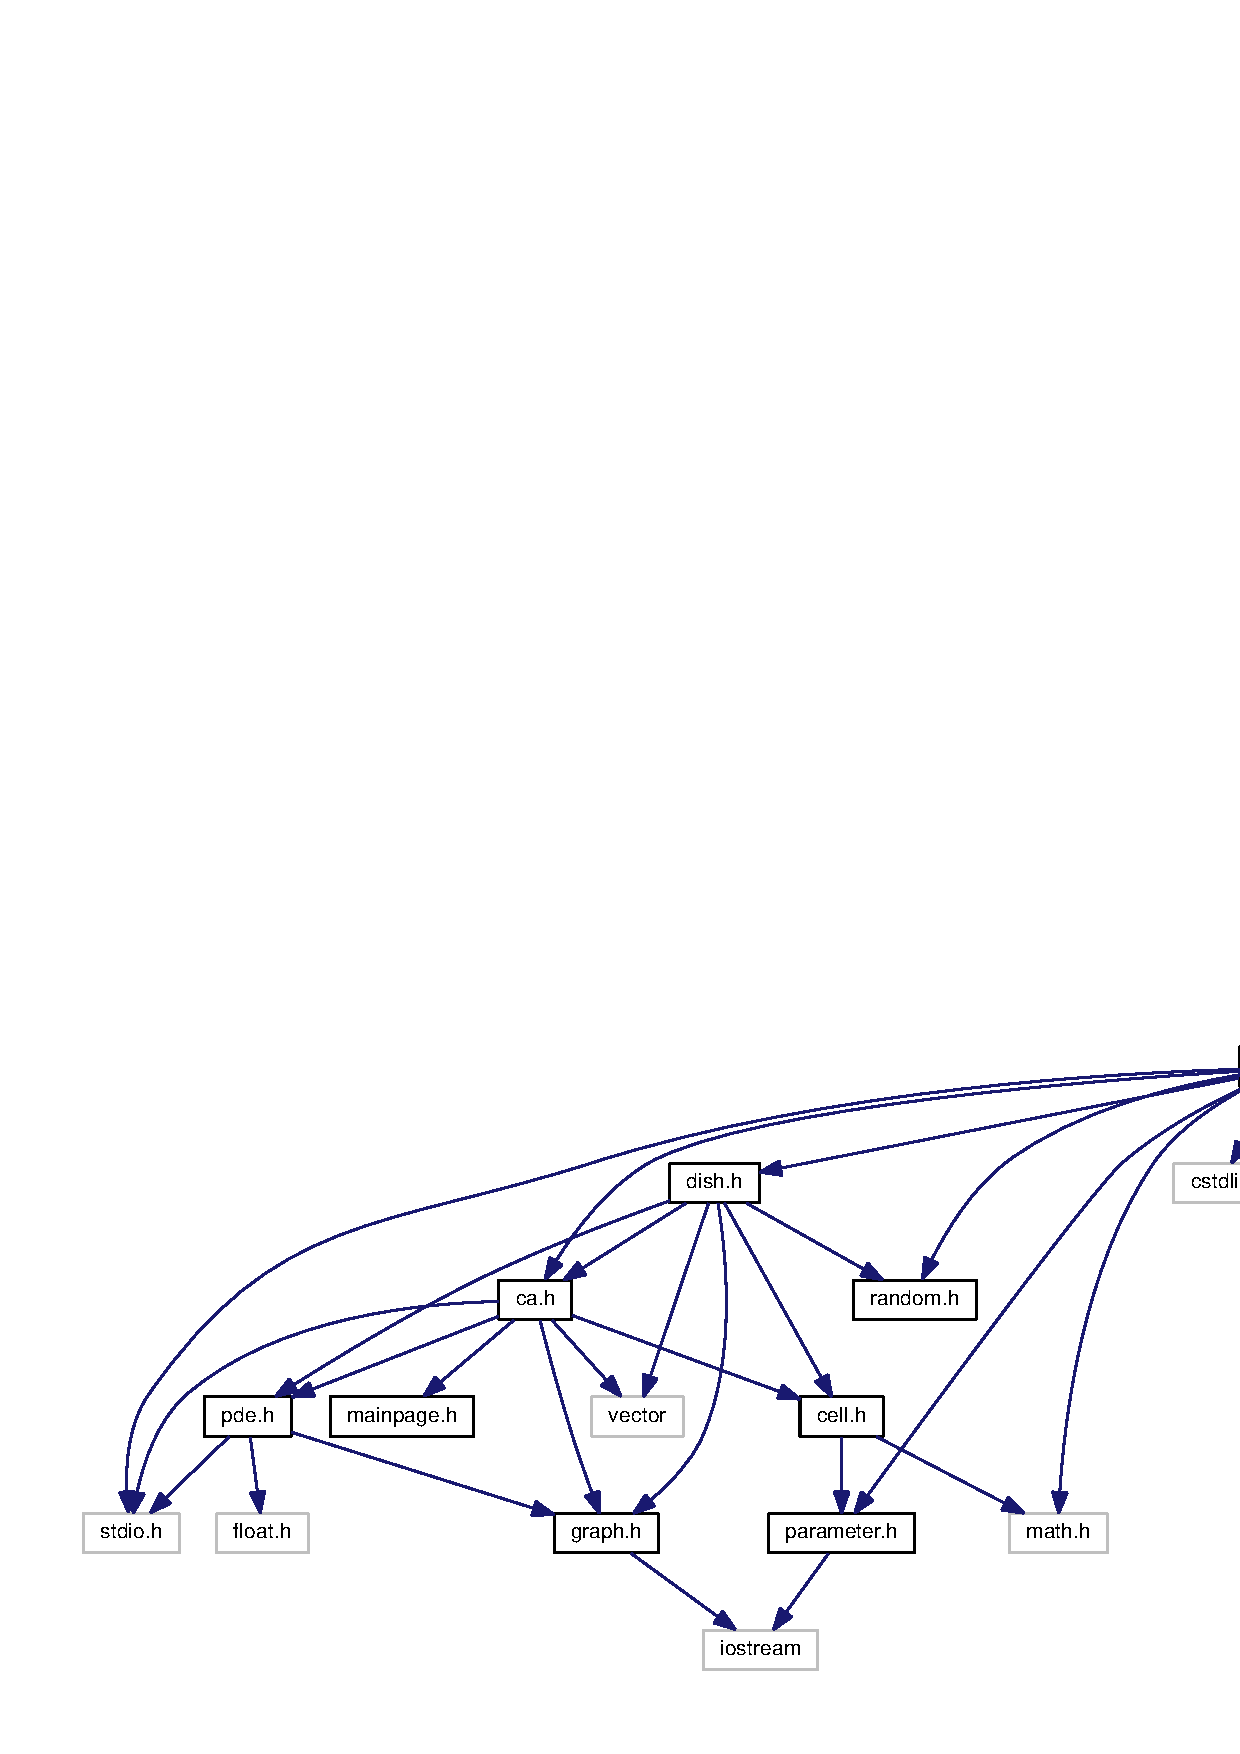
\includegraphics[width=350pt]{ca_8cpp__incl}
\end{center}
\end{figure}
\subsection*{Macros}
\begin{DoxyCompactItemize}
\item 
\#define {\bf Z\-Y\-G\-F\-I\-L\-E}(Z)~$<$Z.\-xpm$>$
\item 
\#define {\bf X\-P\-M}(Z)~Z \#\# \-\_\-xpm
\item 
\#define {\bf Z\-Y\-G\-X\-P\-M}(Z)~{\bf X\-P\-M}(Z)
\item 
\#define {\bf Z\-Y\-G\-O\-T\-E}~init
\end{DoxyCompactItemize}
\subsection*{Functions}
\begin{DoxyCompactItemize}
\item 
double {\bf sat} (double x)
\end{DoxyCompactItemize}
\subsection*{Variables}
\begin{DoxyCompactItemize}
\item 
double {\bf copyprob} [{\bf B\-O\-L\-T\-Z\-M\-A\-N\-N}]
\item 
{\bf Parameter} {\bf par}
\end{DoxyCompactItemize}


\subsection{Macro Definition Documentation}
\index{ca.\-cpp@{ca.\-cpp}!X\-P\-M@{X\-P\-M}}
\index{X\-P\-M@{X\-P\-M}!ca.cpp@{ca.\-cpp}}
\subsubsection[{X\-P\-M}]{\setlength{\rightskip}{0pt plus 5cm}\#define X\-P\-M(
\begin{DoxyParamCaption}
\item[{}]{Z}
\end{DoxyParamCaption}
)~Z \#\# \-\_\-xpm}\label{ca_8cpp_ad195202f179c1ef76500bbe0e69474b8}
\index{ca.\-cpp@{ca.\-cpp}!Z\-Y\-G\-F\-I\-L\-E@{Z\-Y\-G\-F\-I\-L\-E}}
\index{Z\-Y\-G\-F\-I\-L\-E@{Z\-Y\-G\-F\-I\-L\-E}!ca.cpp@{ca.\-cpp}}
\subsubsection[{Z\-Y\-G\-F\-I\-L\-E}]{\setlength{\rightskip}{0pt plus 5cm}\#define Z\-Y\-G\-F\-I\-L\-E(
\begin{DoxyParamCaption}
\item[{}]{Z}
\end{DoxyParamCaption}
)~$<$Z.\-xpm$>$}\label{ca_8cpp_a0340a027666cf38546bcc2b4c6c3f07d}
\index{ca.\-cpp@{ca.\-cpp}!Z\-Y\-G\-O\-T\-E@{Z\-Y\-G\-O\-T\-E}}
\index{Z\-Y\-G\-O\-T\-E@{Z\-Y\-G\-O\-T\-E}!ca.cpp@{ca.\-cpp}}
\subsubsection[{Z\-Y\-G\-O\-T\-E}]{\setlength{\rightskip}{0pt plus 5cm}\#define Z\-Y\-G\-O\-T\-E~init}\label{ca_8cpp_ac02cf23c66d15fb723526d2350a26e43}


Referenced by Cellular\-Potts\-::\-Read\-Zygote\-Picture().

\index{ca.\-cpp@{ca.\-cpp}!Z\-Y\-G\-X\-P\-M@{Z\-Y\-G\-X\-P\-M}}
\index{Z\-Y\-G\-X\-P\-M@{Z\-Y\-G\-X\-P\-M}!ca.cpp@{ca.\-cpp}}
\subsubsection[{Z\-Y\-G\-X\-P\-M}]{\setlength{\rightskip}{0pt plus 5cm}\#define Z\-Y\-G\-X\-P\-M(
\begin{DoxyParamCaption}
\item[{}]{Z}
\end{DoxyParamCaption}
)~{\bf X\-P\-M}(Z)}\label{ca_8cpp_afcc64ea4488ea5d2fd670d5965629262}


Referenced by Cellular\-Potts\-::\-Read\-Zygote\-Picture().



\subsection{Function Documentation}
\index{ca.\-cpp@{ca.\-cpp}!sat@{sat}}
\index{sat@{sat}!ca.cpp@{ca.\-cpp}}
\subsubsection[{sat}]{\setlength{\rightskip}{0pt plus 5cm}double sat (
\begin{DoxyParamCaption}
\item[{double}]{x}
\end{DoxyParamCaption}
)}\label{ca_8cpp_accb67a5931e1b30ac028a9e5af36dd0d}


References Parameter\-::saturation.



\subsection{Variable Documentation}
\index{ca.\-cpp@{ca.\-cpp}!copyprob@{copyprob}}
\index{copyprob@{copyprob}!ca.cpp@{ca.\-cpp}}
\subsubsection[{copyprob}]{\setlength{\rightskip}{0pt plus 5cm}double copyprob[{\bf B\-O\-L\-T\-Z\-M\-A\-N\-N}]}\label{ca_8cpp_aa5a446f73035e36b8932a2d0fd6fde76}
\index{ca.\-cpp@{ca.\-cpp}!par@{par}}
\index{par@{par}!ca.cpp@{ca.\-cpp}}
\subsubsection[{par}]{\setlength{\rightskip}{0pt plus 5cm}{\bf Parameter} par}\label{ca_8cpp_aa11a52593a908c20a7259a3e72c0b348}


Referenced by Qt\-Graphics\-::\-Time\-Step\-Wrap().


\section{ca.\-h File Reference}
\label{ca_8h}\index{ca.\-h@{ca.\-h}}
{\ttfamily \#include \char`\"{}mainpage.\-h\char`\"{}}\\*
{\ttfamily \#include $<$vector$>$}\\*
{\ttfamily \#include $<$stdio.\-h$>$}\\*
{\ttfamily \#include \char`\"{}graph.\-h\char`\"{}}\\*
{\ttfamily \#include \char`\"{}pde.\-h\char`\"{}}\\*
{\ttfamily \#include \char`\"{}cell.\-h\char`\"{}}\\*
Include dependency graph for ca.\-h\-:
\nopagebreak
\begin{figure}[H]
\begin{center}
\leavevmode
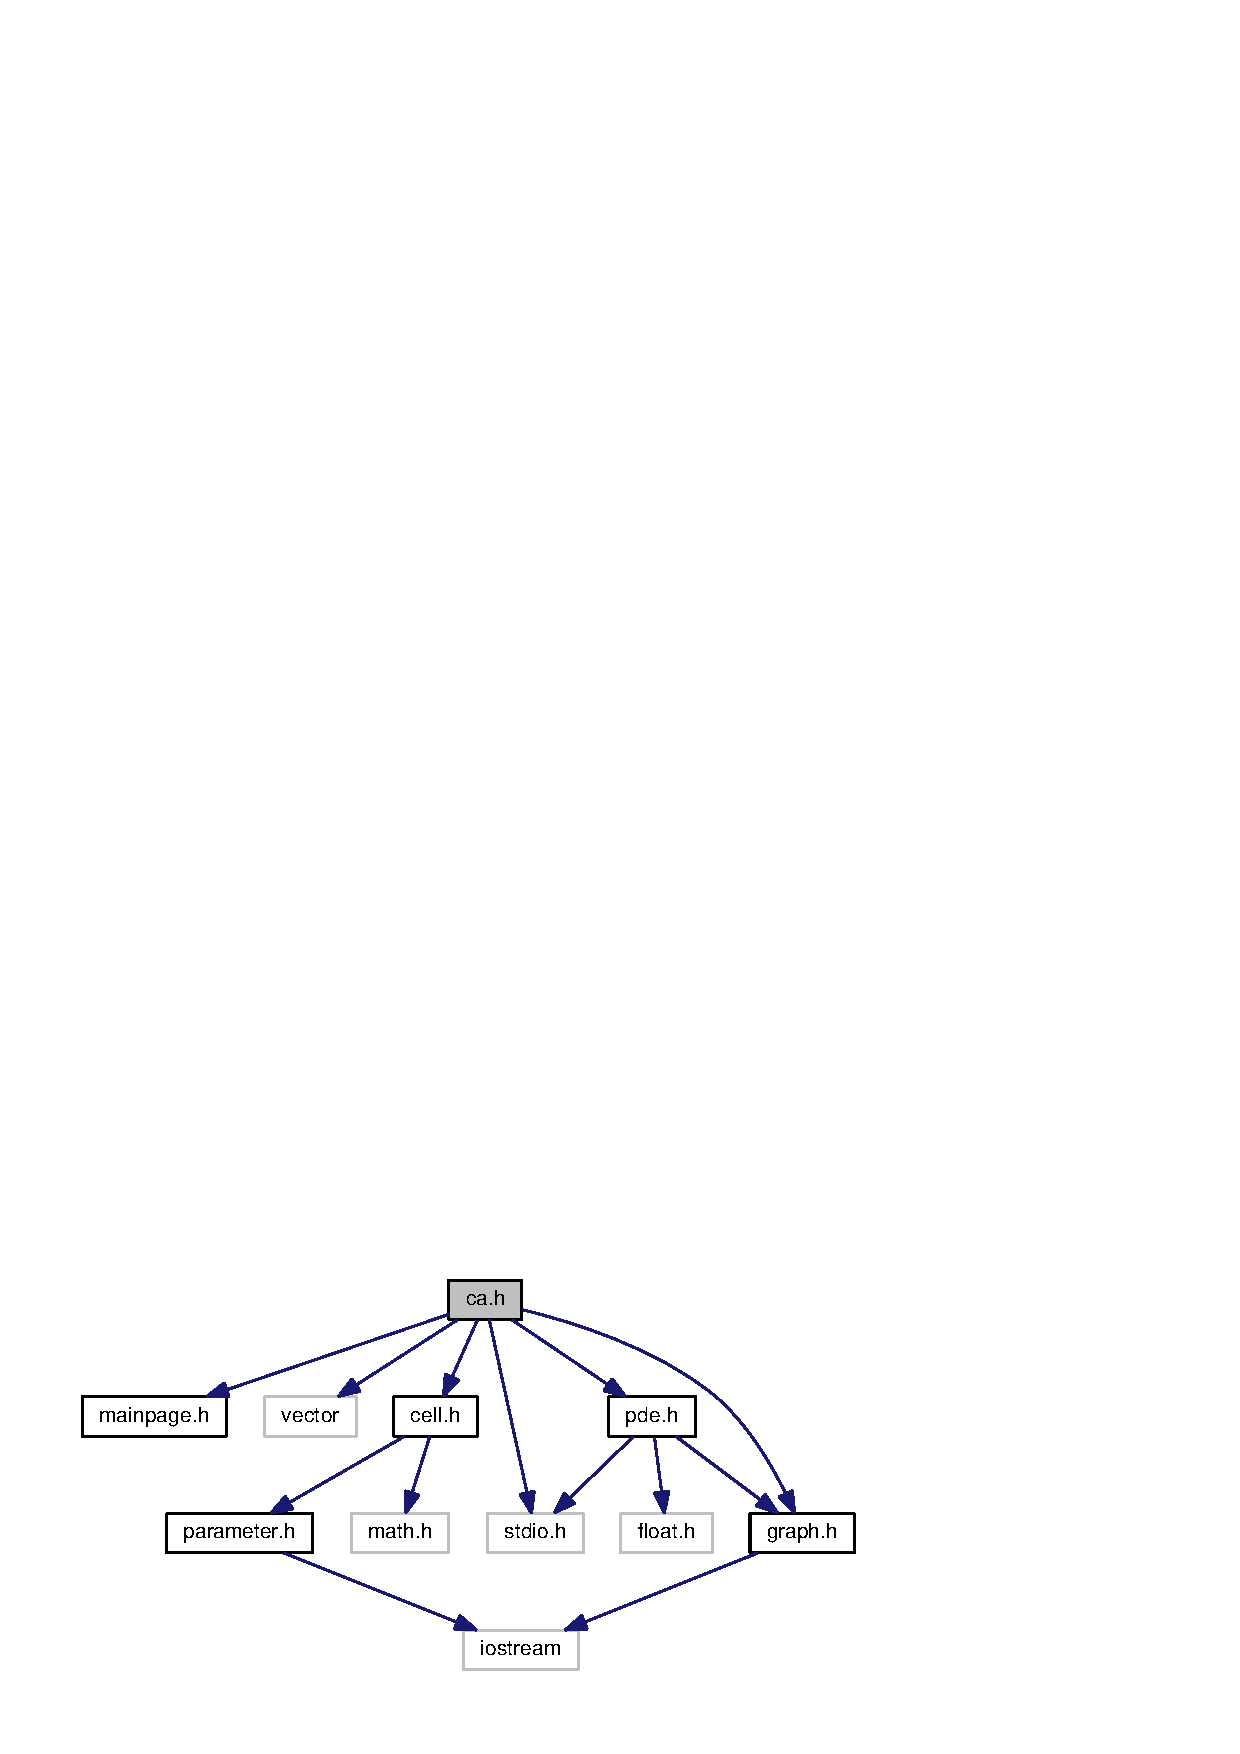
\includegraphics[width=350pt]{ca_8h__incl}
\end{center}
\end{figure}
This graph shows which files directly or indirectly include this file\-:
\nopagebreak
\begin{figure}[H]
\begin{center}
\leavevmode
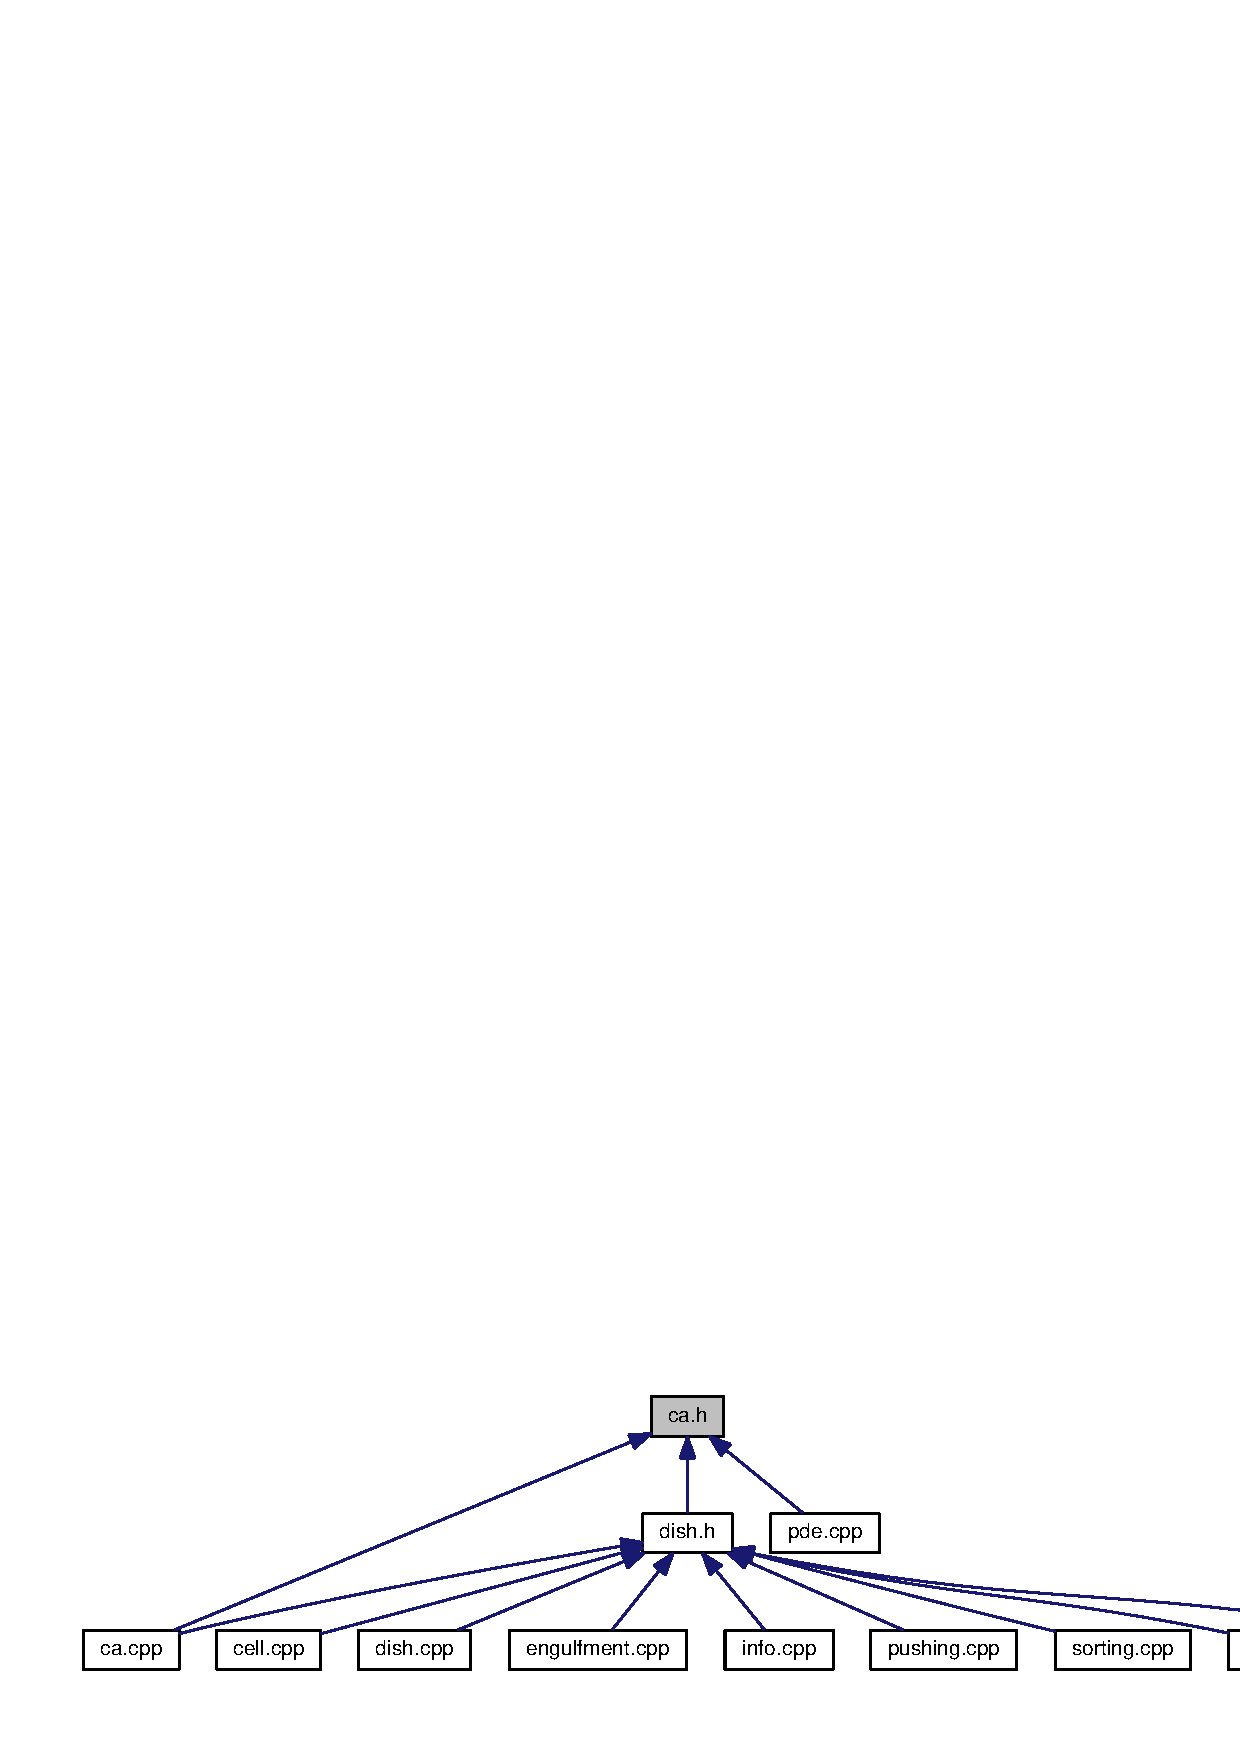
\includegraphics[width=350pt]{ca_8h__dep__incl}
\end{center}
\end{figure}
\subsection*{Classes}
\begin{DoxyCompactItemize}
\item 
class {\bf Dir}
\item 
class {\bf Cellular\-Potts}
\end{DoxyCompactItemize}

\section{cell.\-cpp File Reference}
\label{cell_8cpp}\index{cell.\-cpp@{cell.\-cpp}}
{\ttfamily \#include $<$list$>$}\\*
{\ttfamily \#include $<$vector$>$}\\*
{\ttfamily \#include $<$stdio.\-h$>$}\\*
{\ttfamily \#include $<$fstream$>$}\\*
{\ttfamily \#include $<$malloc.\-h$>$}\\*
{\ttfamily \#include \char`\"{}cell.\-h\char`\"{}}\\*
{\ttfamily \#include \char`\"{}sticky.\-h\char`\"{}}\\*
{\ttfamily \#include \char`\"{}parameter.\-h\char`\"{}}\\*
{\ttfamily \#include \char`\"{}dish.\-h\char`\"{}}\\*
Include dependency graph for cell.\-cpp\-:
\nopagebreak
\begin{figure}[H]
\begin{center}
\leavevmode
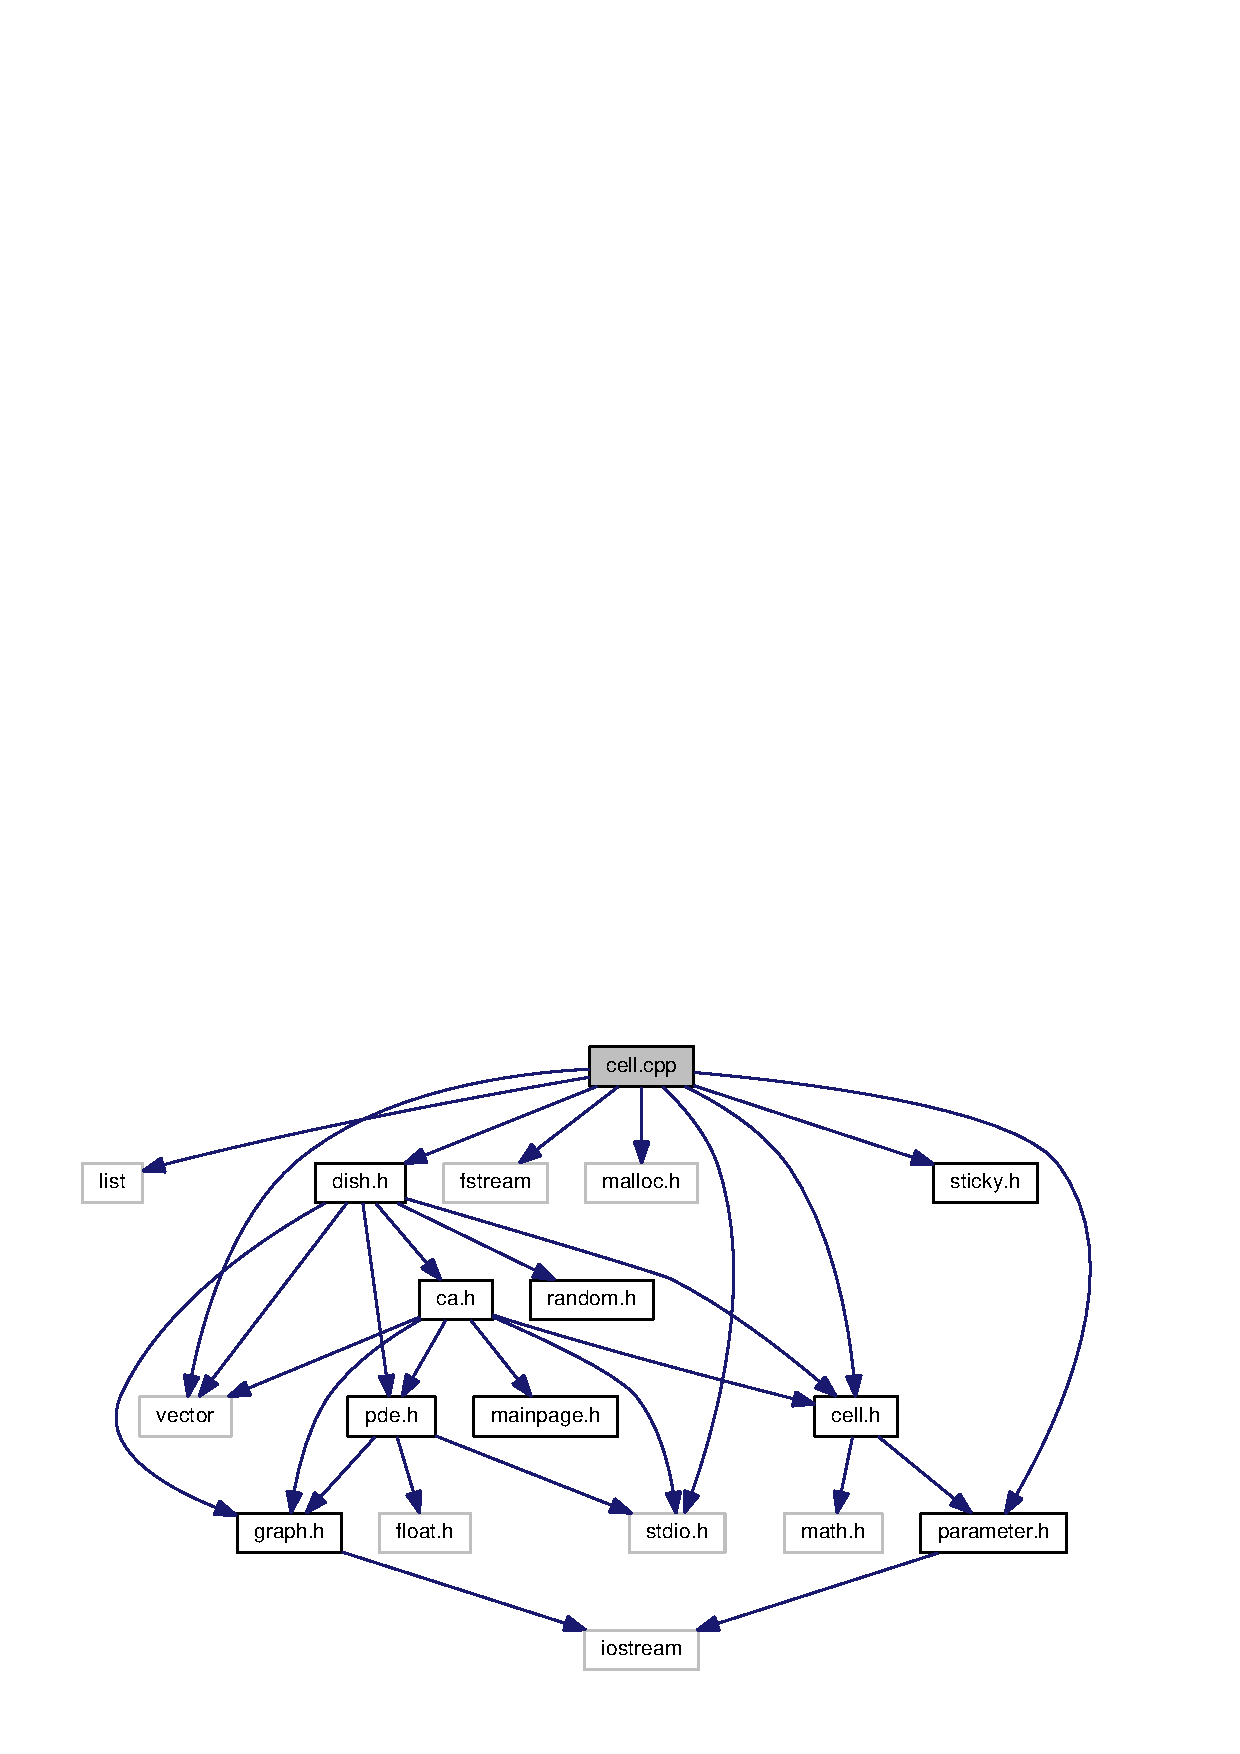
\includegraphics[width=350pt]{cell_8cpp__incl}
\end{center}
\end{figure}
\subsection*{Macros}
\begin{DoxyCompactItemize}
\item 
\#define {\bf H\-A\-S\-H\-C\-O\-L\-N\-U\-M}~255
\end{DoxyCompactItemize}
\subsection*{Variables}
\begin{DoxyCompactItemize}
\item 
{\bf Parameter} {\bf par}
\end{DoxyCompactItemize}


\subsection{Macro Definition Documentation}
\index{cell.\-cpp@{cell.\-cpp}!H\-A\-S\-H\-C\-O\-L\-N\-U\-M@{H\-A\-S\-H\-C\-O\-L\-N\-U\-M}}
\index{H\-A\-S\-H\-C\-O\-L\-N\-U\-M@{H\-A\-S\-H\-C\-O\-L\-N\-U\-M}!cell.cpp@{cell.\-cpp}}
\subsubsection[{H\-A\-S\-H\-C\-O\-L\-N\-U\-M}]{\setlength{\rightskip}{0pt plus 5cm}\#define H\-A\-S\-H\-C\-O\-L\-N\-U\-M~255}\label{cell_8cpp_a4af06ace089d6565d5478df65ebecae5}


\subsection{Variable Documentation}
\index{cell.\-cpp@{cell.\-cpp}!par@{par}}
\index{par@{par}!cell.cpp@{cell.\-cpp}}
\subsubsection[{par}]{\setlength{\rightskip}{0pt plus 5cm}{\bf Parameter} par}\label{cell_8cpp_aa11a52593a908c20a7259a3e72c0b348}

\section{cell.\-h File Reference}
\label{cell_8h}\index{cell.\-h@{cell.\-h}}
{\ttfamily \#include \char`\"{}parameter.\-h\char`\"{}}\\*
{\ttfamily \#include $<$math.\-h$>$}\\*
Include dependency graph for cell.\-h\-:
\nopagebreak
\begin{figure}[H]
\begin{center}
\leavevmode
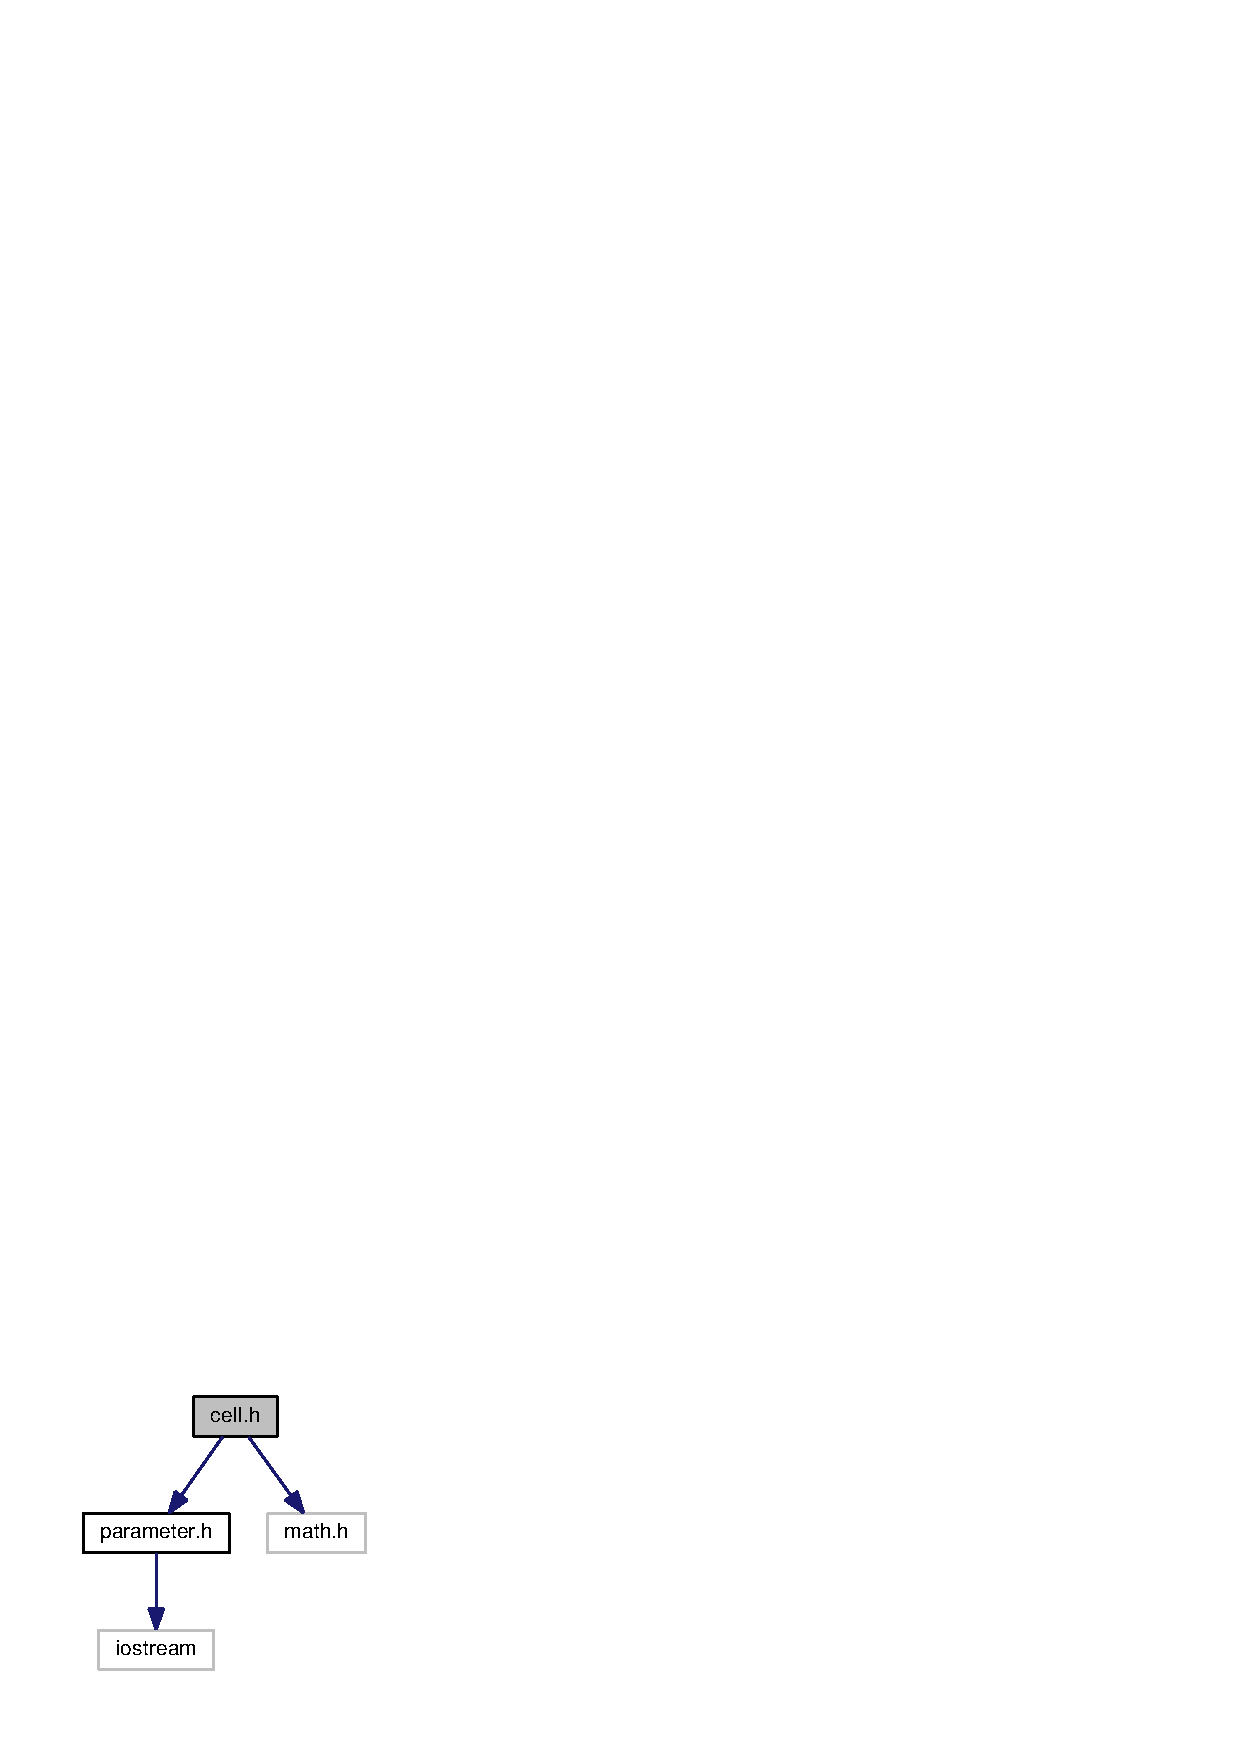
\includegraphics[width=179pt]{cell_8h__incl}
\end{center}
\end{figure}
This graph shows which files directly or indirectly include this file\-:
\nopagebreak
\begin{figure}[H]
\begin{center}
\leavevmode
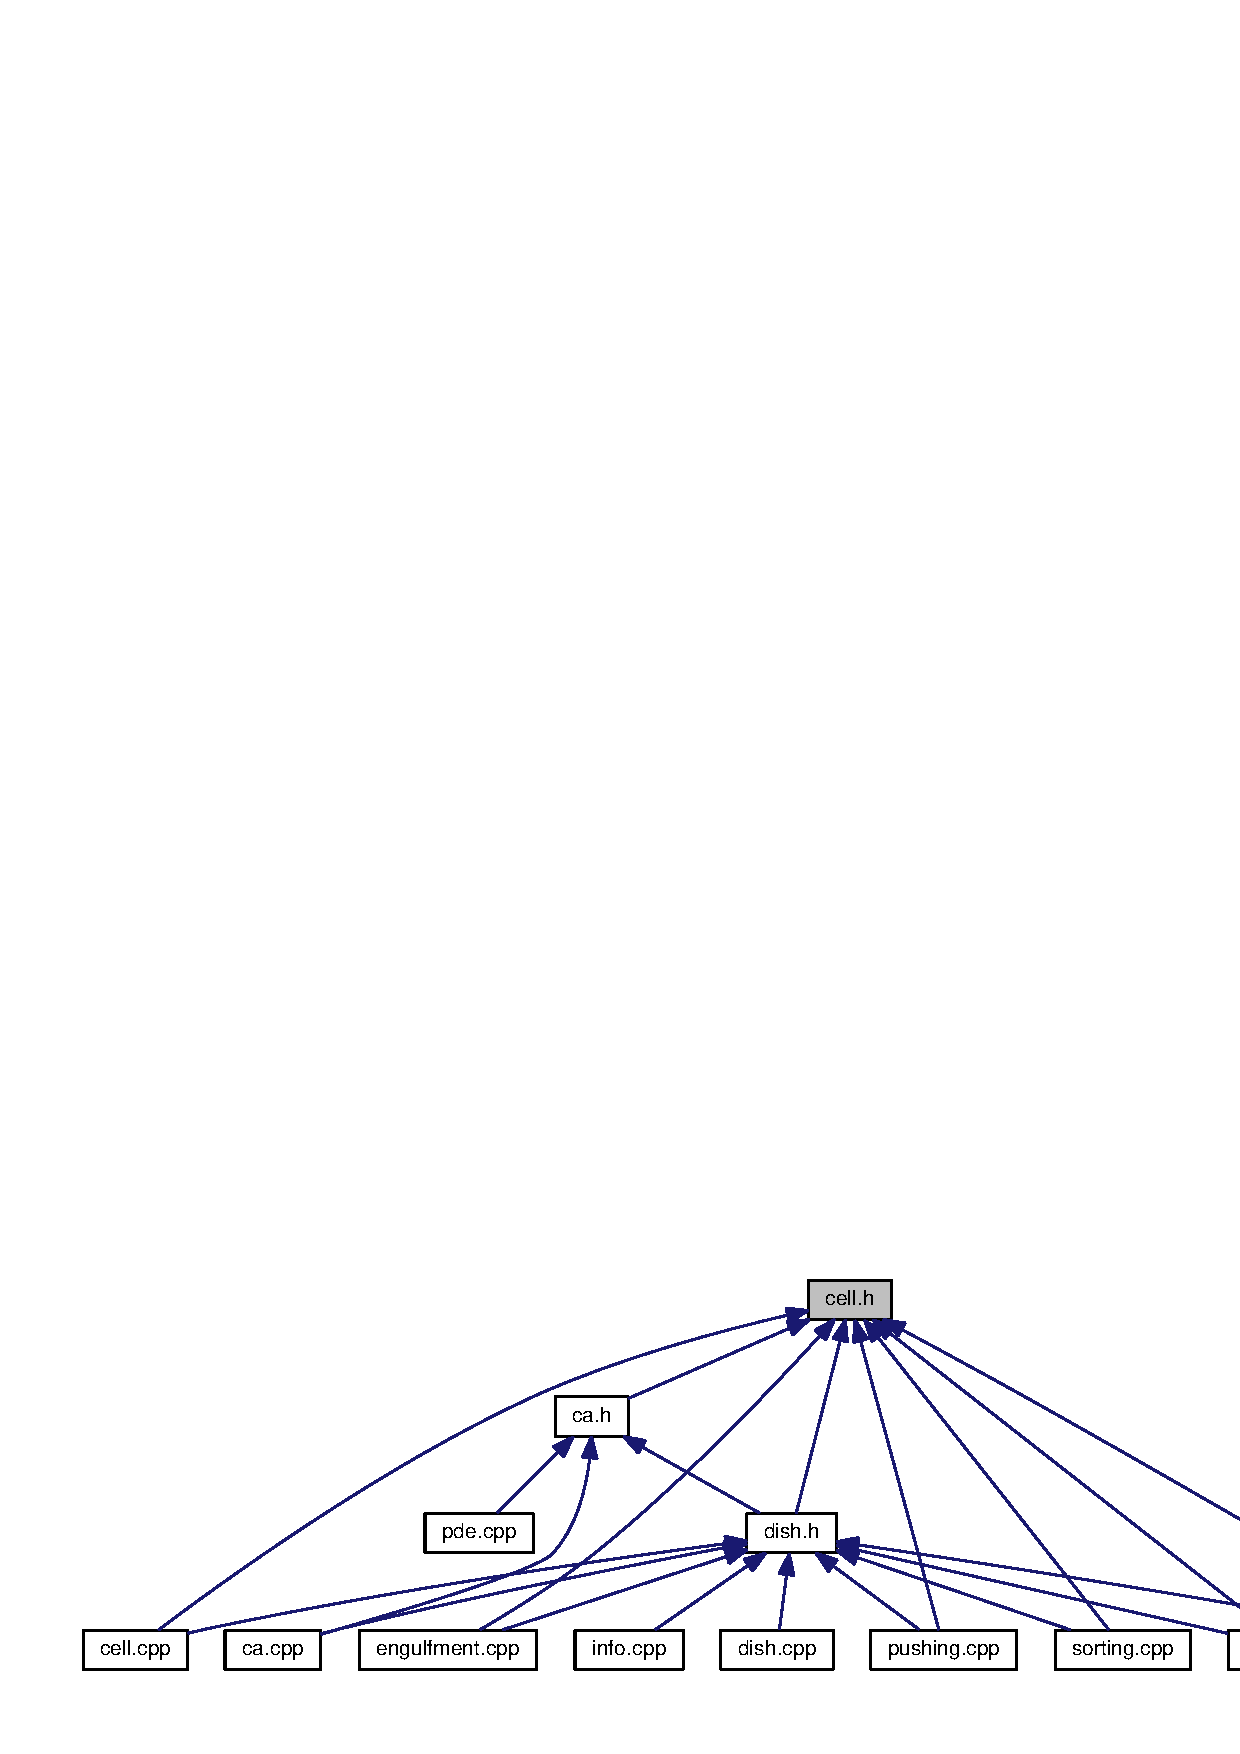
\includegraphics[width=350pt]{cell_8h__dep__incl}
\end{center}
\end{figure}
\subsection*{Classes}
\begin{DoxyCompactItemize}
\item 
class {\bf Cell}
\end{DoxyCompactItemize}
\subsection*{Variables}
\begin{DoxyCompactItemize}
\item 
{\bf Parameter} {\bf par}
\end{DoxyCompactItemize}


\subsection{Variable Documentation}
\index{cell.\-h@{cell.\-h}!par@{par}}
\index{par@{par}!cell.h@{cell.\-h}}
\subsubsection[{par}]{\setlength{\rightskip}{0pt plus 5cm}{\bf Parameter} par}\label{cell_8h_aa11a52593a908c20a7259a3e72c0b348}

\section{conrec.\-cpp File Reference}
\label{conrec_8cpp}\index{conrec.\-cpp@{conrec.\-cpp}}
{\ttfamily \#include $<$stdio.\-h$>$}\\*
{\ttfamily \#include $<$math.\-h$>$}\\*
{\ttfamily \#include \char`\"{}graph.\-h\char`\"{}}\\*
{\ttfamily \#include \char`\"{}conrec.\-h\char`\"{}}\\*
Include dependency graph for conrec.\-cpp\-:
\nopagebreak
\begin{figure}[H]
\begin{center}
\leavevmode
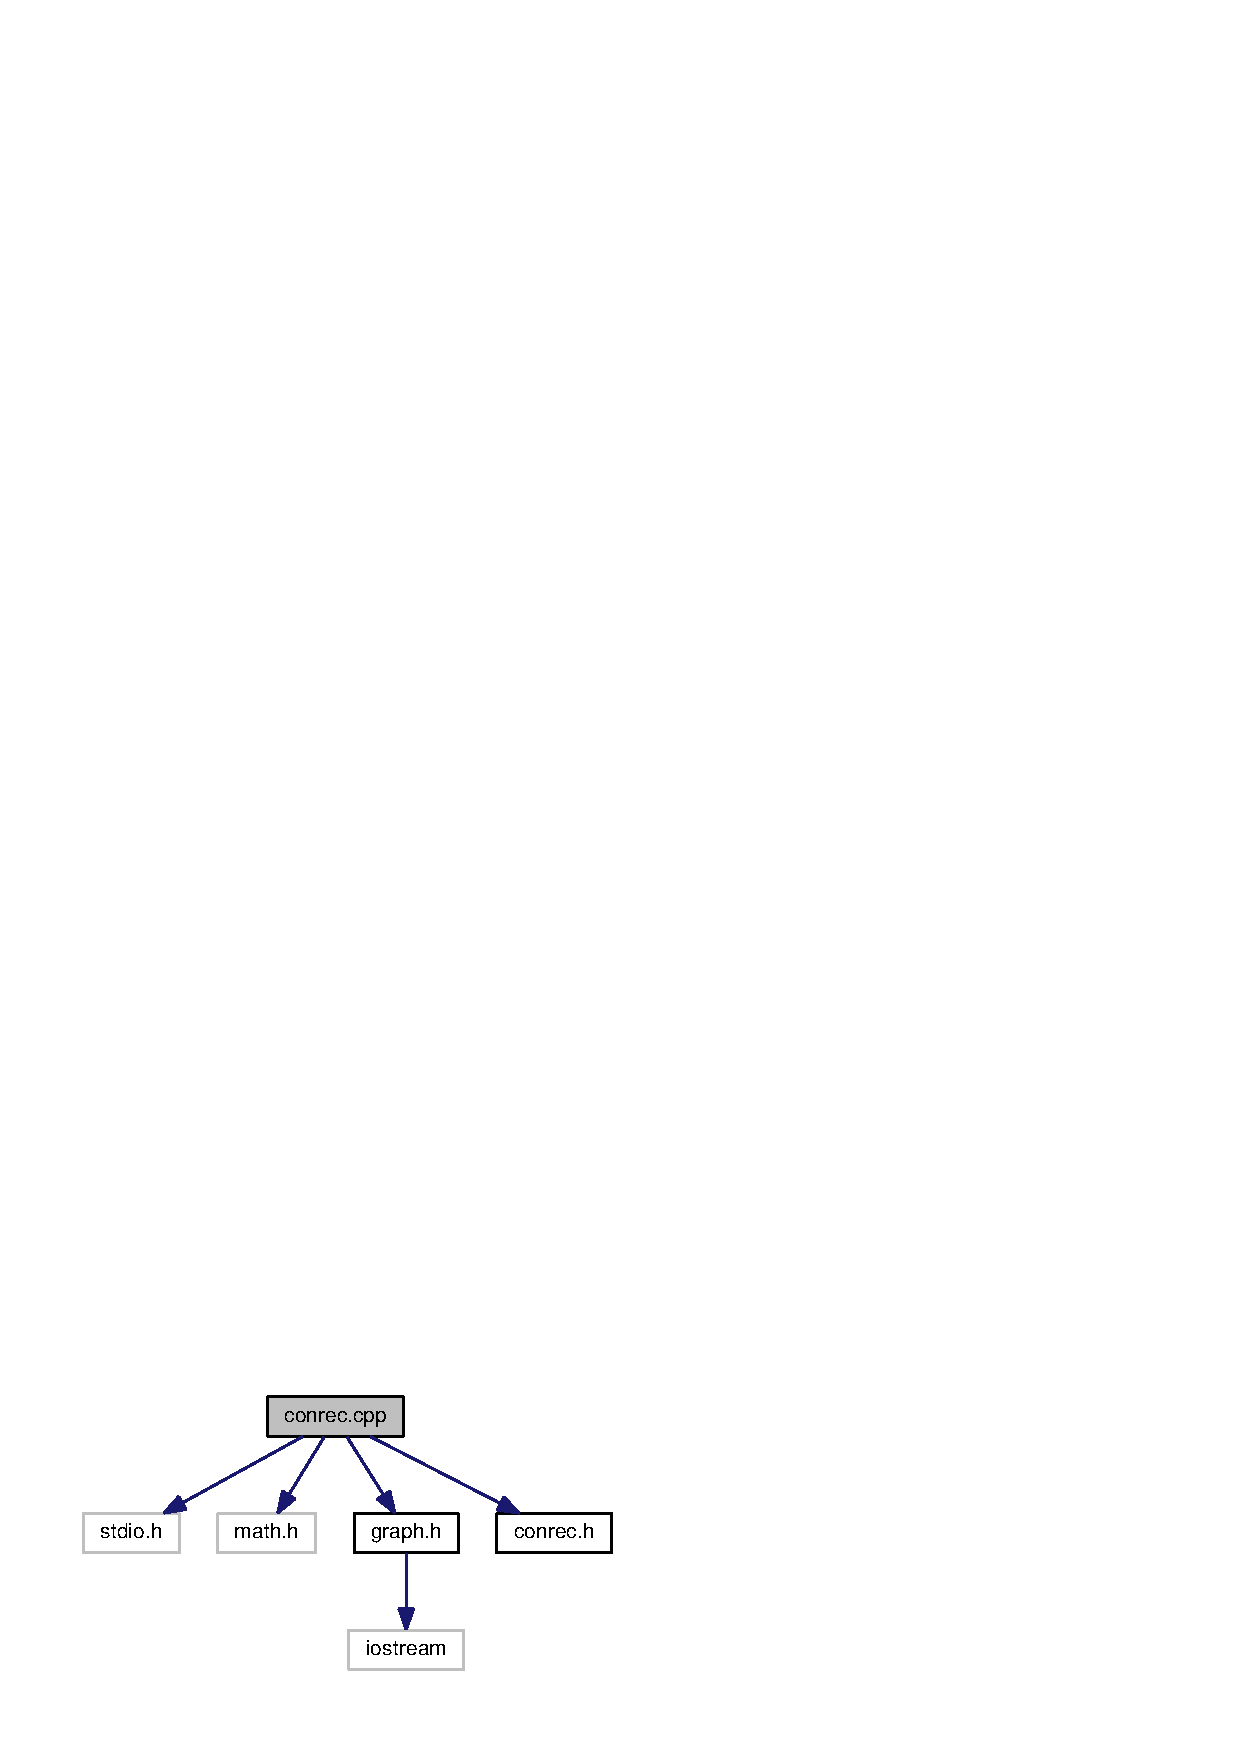
\includegraphics[width=297pt]{conrec_8cpp__incl}
\end{center}
\end{figure}
\subsection*{Macros}
\begin{DoxyCompactItemize}
\item 
\#define {\bf xsect}(p1, p2)~(h[p2]$\ast$xh[p1]-\/h[p1]$\ast$xh[p2])/(h[p2]-\/h[p1])
\item 
\#define {\bf ysect}(p1, p2)~(h[p2]$\ast$yh[p1]-\/h[p1]$\ast$yh[p2])/(h[p2]-\/h[p1])
\item 
\#define {\bf min}(x, y)~(x$<$y?x\-:y)
\item 
\#define {\bf max}(x, y)~(x$>$y?x\-:y)
\end{DoxyCompactItemize}
\subsection*{Functions}
\begin{DoxyCompactItemize}
\item 
int {\bf conrec} (double $\ast$$\ast$d, int ilb, int iub, int jlb, int jub, double $\ast$x, double $\ast$y, int nc, double $\ast$z, {\bf Graphics} $\ast$g, int colour)
\begin{DoxyCompactList}\small\item\em Paul Bourke's conrec algorithm to draw contour lines of \doxyref{P\-D\-E}{p.}{classPDE} fields. \end{DoxyCompactList}\end{DoxyCompactItemize}


\subsection{Macro Definition Documentation}
\index{conrec.\-cpp@{conrec.\-cpp}!max@{max}}
\index{max@{max}!conrec.cpp@{conrec.\-cpp}}
\subsubsection[{max}]{\setlength{\rightskip}{0pt plus 5cm}\#define max(
\begin{DoxyParamCaption}
\item[{}]{x, }
\item[{}]{y}
\end{DoxyParamCaption}
)~(x$>$y?x\-:y)}\label{conrec_8cpp_ac39d9cef6a5e030ba8d9e11121054268}


Referenced by conrec(), P\-D\-E\-::\-Contour\-Plot(), and P\-D\-E\-::\-Max().

\index{conrec.\-cpp@{conrec.\-cpp}!min@{min}}
\index{min@{min}!conrec.cpp@{conrec.\-cpp}}
\subsubsection[{min}]{\setlength{\rightskip}{0pt plus 5cm}\#define min(
\begin{DoxyParamCaption}
\item[{}]{x, }
\item[{}]{y}
\end{DoxyParamCaption}
)~(x$<$y?x\-:y)}\label{conrec_8cpp_abb702d8b501669a23aa0ab3b281b9384}


Referenced by conrec(), P\-D\-E\-::\-Contour\-Plot(), and P\-D\-E\-::\-Min().

\index{conrec.\-cpp@{conrec.\-cpp}!xsect@{xsect}}
\index{xsect@{xsect}!conrec.cpp@{conrec.\-cpp}}
\subsubsection[{xsect}]{\setlength{\rightskip}{0pt plus 5cm}\#define xsect(
\begin{DoxyParamCaption}
\item[{}]{p1, }
\item[{}]{p2}
\end{DoxyParamCaption}
)~(h[p2]$\ast$xh[p1]-\/h[p1]$\ast$xh[p2])/(h[p2]-\/h[p1])}\label{conrec_8cpp_a1945de04712b1719569931533875fddc}


Referenced by conrec().

\index{conrec.\-cpp@{conrec.\-cpp}!ysect@{ysect}}
\index{ysect@{ysect}!conrec.cpp@{conrec.\-cpp}}
\subsubsection[{ysect}]{\setlength{\rightskip}{0pt plus 5cm}\#define ysect(
\begin{DoxyParamCaption}
\item[{}]{p1, }
\item[{}]{p2}
\end{DoxyParamCaption}
)~(h[p2]$\ast$yh[p1]-\/h[p1]$\ast$yh[p2])/(h[p2]-\/h[p1])}\label{conrec_8cpp_a9280aea3f72512414a0ac224816b2604}


Referenced by conrec().



\subsection{Function Documentation}
\index{conrec.\-cpp@{conrec.\-cpp}!conrec@{conrec}}
\index{conrec@{conrec}!conrec.cpp@{conrec.\-cpp}}
\subsubsection[{conrec}]{\setlength{\rightskip}{0pt plus 5cm}int conrec (
\begin{DoxyParamCaption}
\item[{double $\ast$$\ast$}]{d, }
\item[{int}]{ilb, }
\item[{int}]{iub, }
\item[{int}]{jlb, }
\item[{int}]{jub, }
\item[{double $\ast$}]{x, }
\item[{double $\ast$}]{y, }
\item[{int}]{nc, }
\item[{double $\ast$}]{z, }
\item[{{\bf Graphics} $\ast$}]{g, }
\item[{int}]{colour = {\ttfamily 1}}
\end{DoxyParamCaption}
)}\label{conrec_8cpp_a6e7a0b7c5669bfd7cd8b598d97a599c4}


Paul Bourke's conrec algorithm to draw contour lines of \doxyref{P\-D\-E}{p.}{classPDE} fields. 

C-\/code Copyright (c) 1996-\/1997 Nicholas Yue. 

References max, min, Graphics\-::\-Point(), xsect, and ysect.



Referenced by P\-D\-E\-::\-Contour\-Plot().


\section{conrec.\-h File Reference}
\label{conrec_8h}\index{conrec.\-h@{conrec.\-h}}
This graph shows which files directly or indirectly include this file\-:
\nopagebreak
\begin{figure}[H]
\begin{center}
\leavevmode
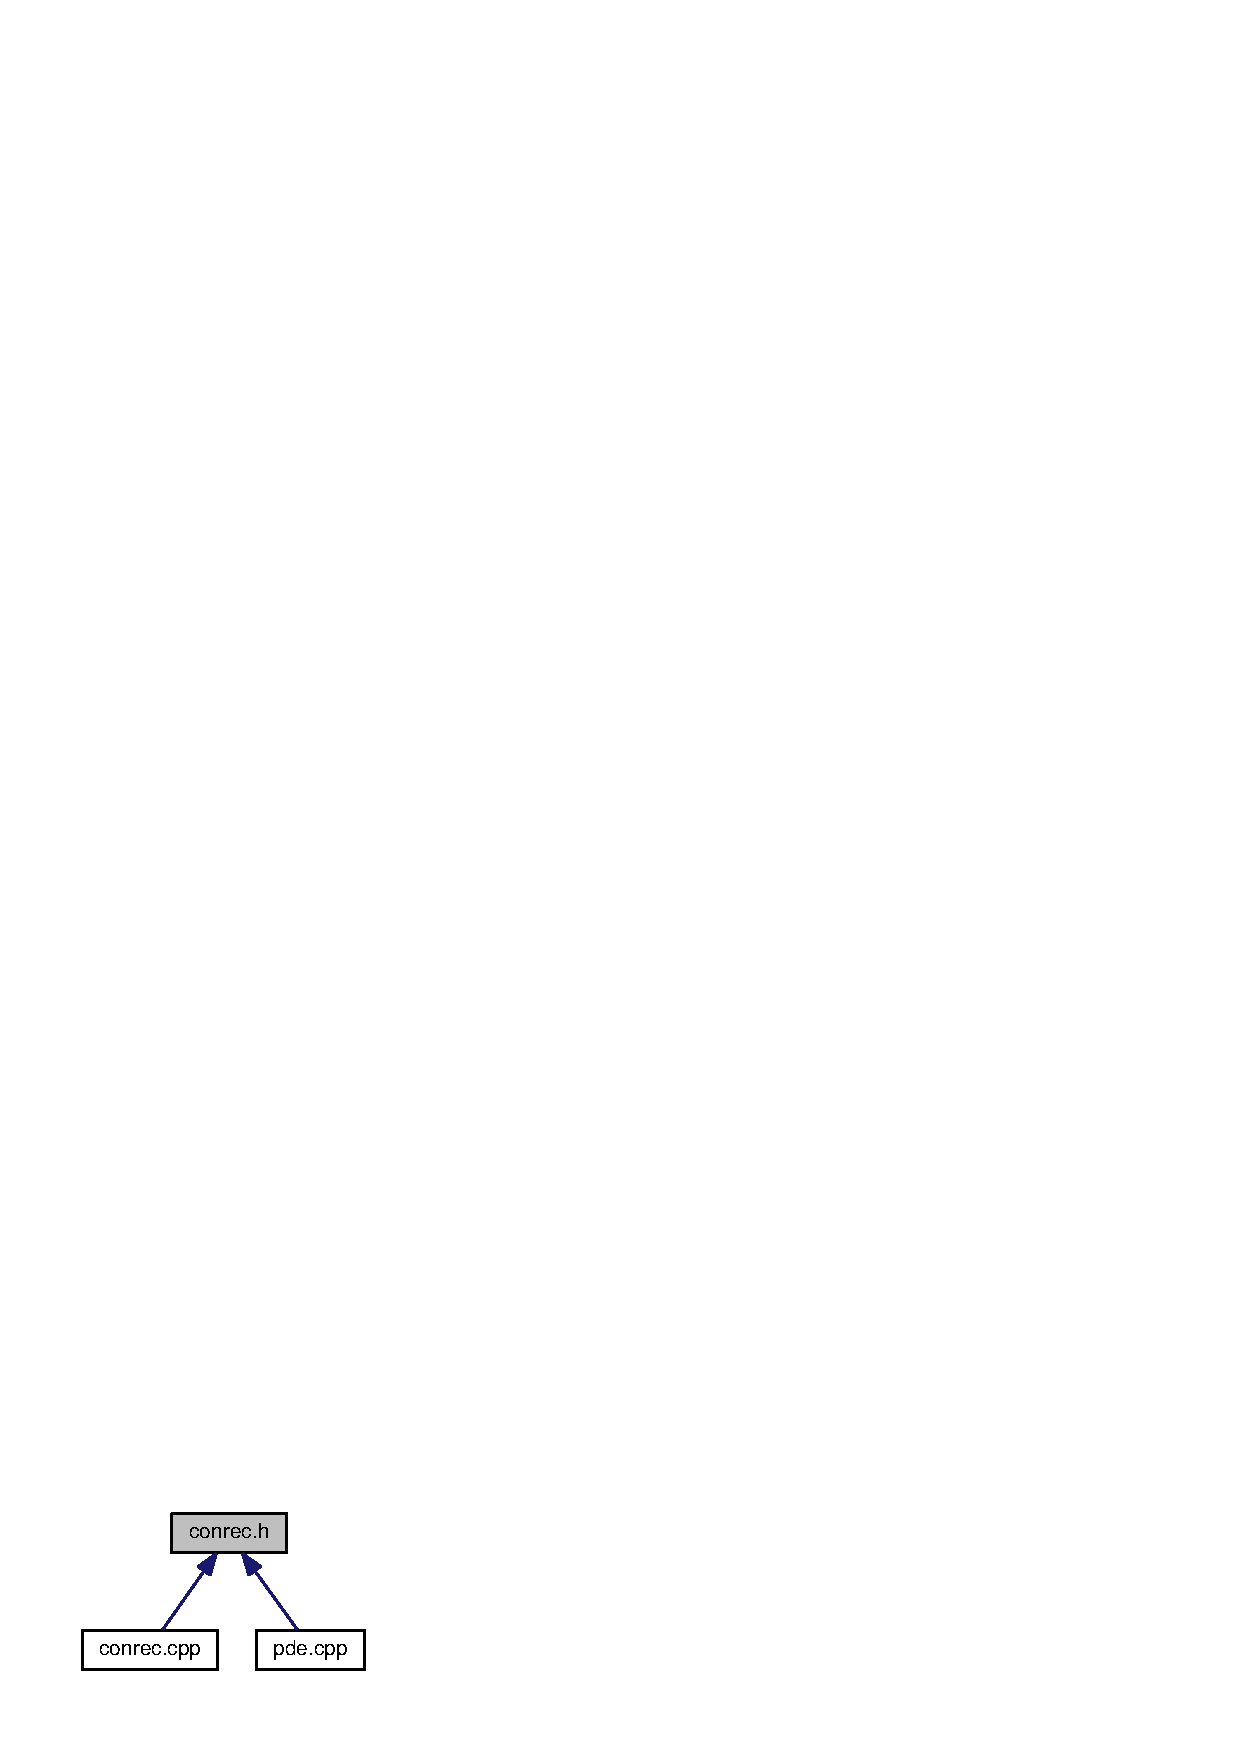
\includegraphics[width=179pt]{conrec_8h__dep__incl}
\end{center}
\end{figure}
\subsection*{Functions}
\begin{DoxyCompactItemize}
\item 
int {\bf conrec} (double $\ast$$\ast$d, int ilb, int iub, int jlb, int jub, double $\ast$x, double $\ast$y, int nc, double $\ast$z, {\bf Graphics} $\ast$g, int colour=1)
\begin{DoxyCompactList}\small\item\em Paul Bourke's conrec algorithm to draw contour lines of \doxyref{P\-D\-E}{p.}{classPDE} fields. \end{DoxyCompactList}\end{DoxyCompactItemize}


\subsection{Function Documentation}
\index{conrec.\-h@{conrec.\-h}!conrec@{conrec}}
\index{conrec@{conrec}!conrec.h@{conrec.\-h}}
\subsubsection[{conrec}]{\setlength{\rightskip}{0pt plus 5cm}int conrec (
\begin{DoxyParamCaption}
\item[{double $\ast$$\ast$}]{d, }
\item[{int}]{ilb, }
\item[{int}]{iub, }
\item[{int}]{jlb, }
\item[{int}]{jub, }
\item[{double $\ast$}]{x, }
\item[{double $\ast$}]{y, }
\item[{int}]{nc, }
\item[{double $\ast$}]{z, }
\item[{{\bf Graphics} $\ast$}]{g, }
\item[{int}]{colour = {\ttfamily 1}}
\end{DoxyParamCaption}
)}\label{conrec_8h_a7da5dc0856966b48ec671c4fb42fb524}


Paul Bourke's conrec algorithm to draw contour lines of \doxyref{P\-D\-E}{p.}{classPDE} fields. 

C-\/code Copyright (c) 1996-\/1997 Nicholas Yue. 

References max, min, Graphics\-::\-Point(), xsect, and ysect.



Referenced by P\-D\-E\-::\-Contour\-Plot().


\section{crash.\-cpp File Reference}
\label{crash_8cpp}\index{crash.\-cpp@{crash.\-cpp}}
{\ttfamily \#include $<$signal.\-h$>$}\\*
{\ttfamily \#include $<$stdio.\-h$>$}\\*
{\ttfamily \#include $<$stdlib.\-h$>$}\\*
{\ttfamily \#include $<$malloc.\-h$>$}\\*
{\ttfamily \#include $<$string.\-h$>$}\\*
{\ttfamily \#include \char`\"{}sticky.\-h\char`\"{}}\\*
{\ttfamily \#include \char`\"{}crash.\-h\char`\"{}}\\*
Include dependency graph for crash.\-cpp\-:
\nopagebreak
\begin{figure}[H]
\begin{center}
\leavevmode
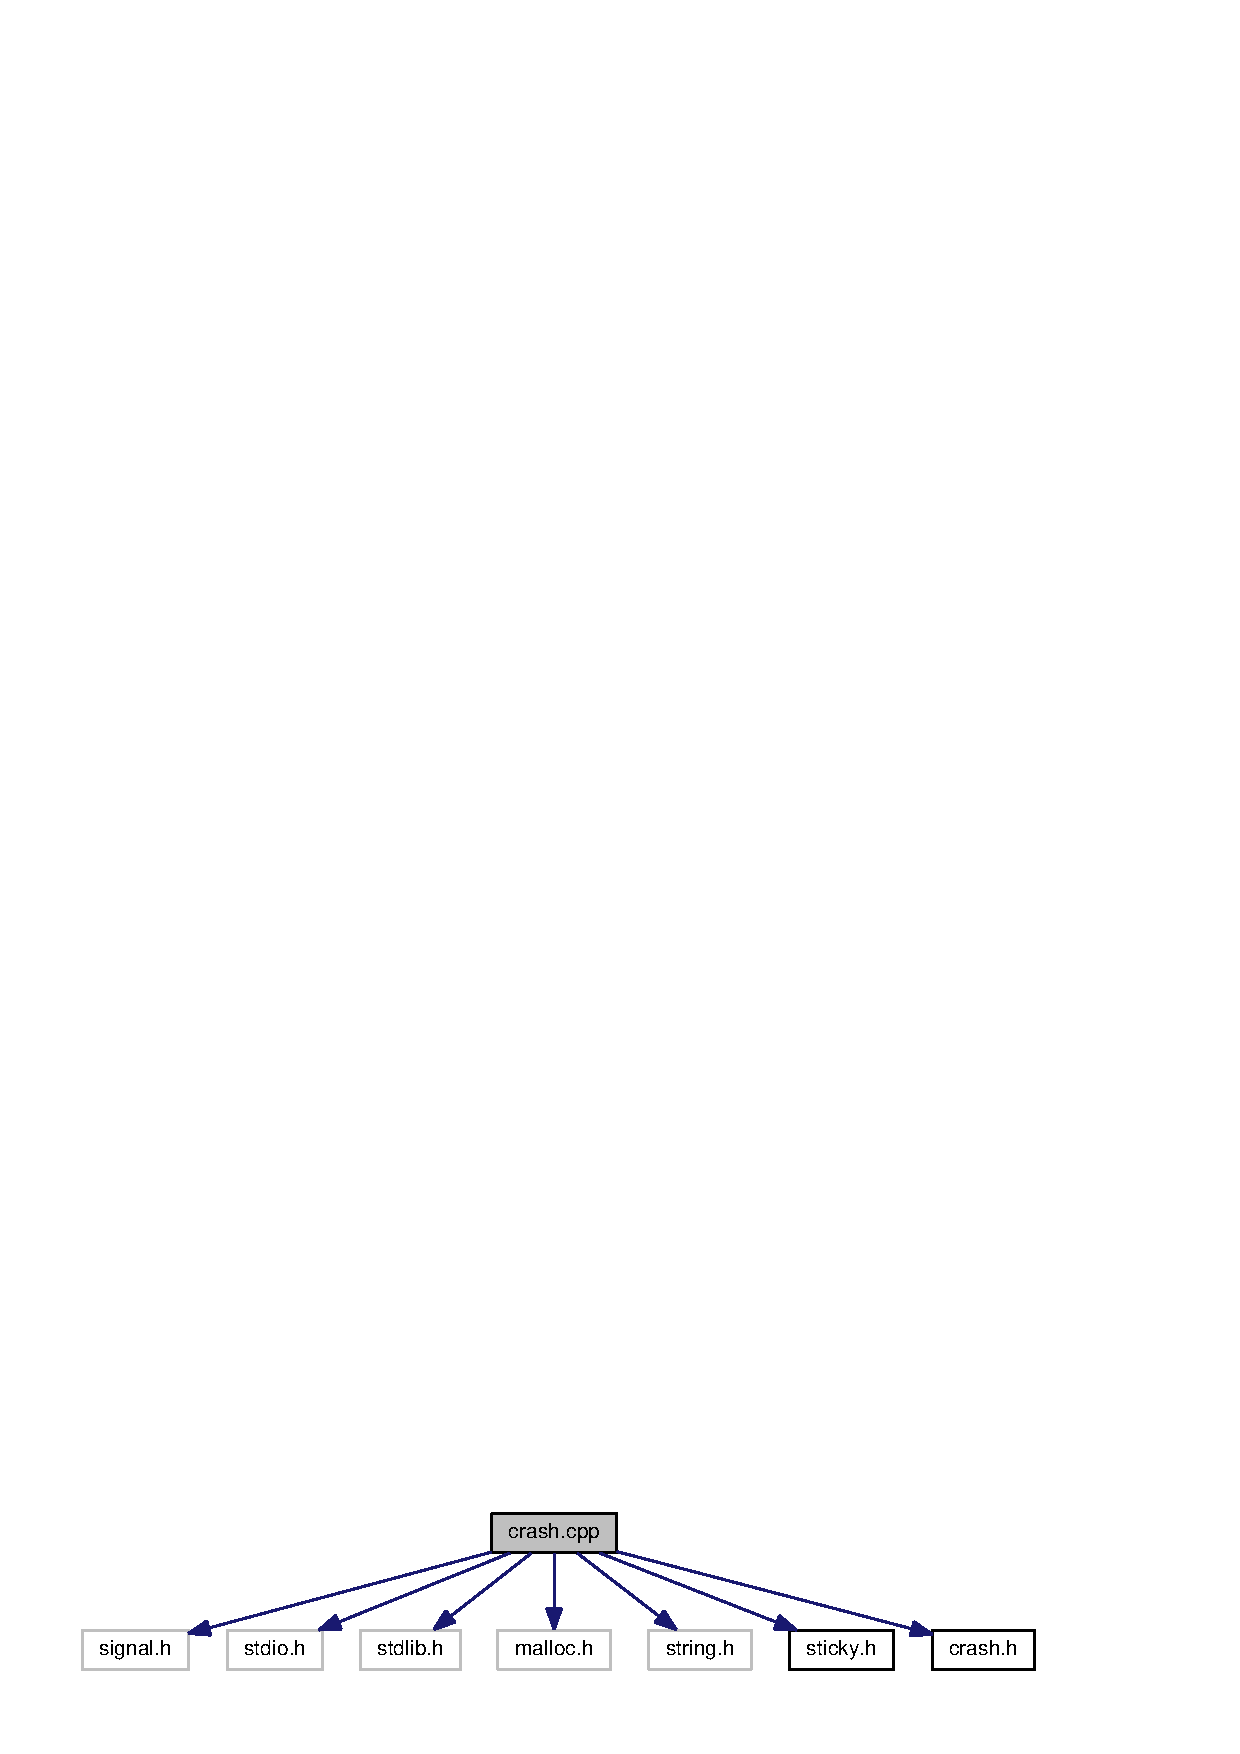
\includegraphics[width=350pt]{crash_8cpp__incl}
\end{center}
\end{figure}
\subsection*{Macros}
\begin{DoxyCompactItemize}
\item 
\#define {\bf N\-O\-P\-V\-M}
\end{DoxyCompactItemize}
\subsection*{Functions}
\begin{DoxyCompactItemize}
\item 
void {\bf Start\-S\-I\-G\-I\-N\-T\-Handling} ()
\item 
void {\bf Handle\-S\-I\-G\-I\-N\-T} (int dummy)
\item 
void {\bf Start\-S\-I\-G\-S\-E\-G\-V\-Handling} ()
\item 
void {\bf Handle\-S\-I\-G\-S\-E\-G\-V} (int dummy)
\item 
void {\bf Nice\-Message} ()
\item 
void {\bf Memory\-Warning} (void)
\item 
void {\bf Crash} (char $\ast$message)
\end{DoxyCompactItemize}


\subsection{Macro Definition Documentation}
\index{crash.\-cpp@{crash.\-cpp}!N\-O\-P\-V\-M@{N\-O\-P\-V\-M}}
\index{N\-O\-P\-V\-M@{N\-O\-P\-V\-M}!crash.cpp@{crash.\-cpp}}
\subsubsection[{N\-O\-P\-V\-M}]{\setlength{\rightskip}{0pt plus 5cm}\#define N\-O\-P\-V\-M}\label{crash_8cpp_affeb851a50e0fe35fa29a8b04113bcf1}


\subsection{Function Documentation}
\index{crash.\-cpp@{crash.\-cpp}!Crash@{Crash}}
\index{Crash@{Crash}!crash.cpp@{crash.\-cpp}}
\subsubsection[{Crash}]{\setlength{\rightskip}{0pt plus 5cm}void Crash (
\begin{DoxyParamCaption}
\item[{char $\ast$}]{message}
\end{DoxyParamCaption}
)}\label{crash_8cpp_aa1a68e59048ea7e4b1e8ec147425715f}


Referenced by Handle\-S\-I\-G\-I\-N\-T(), Handle\-S\-I\-G\-S\-E\-G\-V(), and Memory\-Warning().

\index{crash.\-cpp@{crash.\-cpp}!Handle\-S\-I\-G\-I\-N\-T@{Handle\-S\-I\-G\-I\-N\-T}}
\index{Handle\-S\-I\-G\-I\-N\-T@{Handle\-S\-I\-G\-I\-N\-T}!crash.cpp@{crash.\-cpp}}
\subsubsection[{Handle\-S\-I\-G\-I\-N\-T}]{\setlength{\rightskip}{0pt plus 5cm}void Handle\-S\-I\-G\-I\-N\-T (
\begin{DoxyParamCaption}
\item[{int}]{dummy}
\end{DoxyParamCaption}
)}\label{crash_8cpp_a9204dc74d558cf88808a07563c0720e7}


References Crash().



Referenced by Start\-S\-I\-G\-I\-N\-T\-Handling().

\index{crash.\-cpp@{crash.\-cpp}!Handle\-S\-I\-G\-S\-E\-G\-V@{Handle\-S\-I\-G\-S\-E\-G\-V}}
\index{Handle\-S\-I\-G\-S\-E\-G\-V@{Handle\-S\-I\-G\-S\-E\-G\-V}!crash.cpp@{crash.\-cpp}}
\subsubsection[{Handle\-S\-I\-G\-S\-E\-G\-V}]{\setlength{\rightskip}{0pt plus 5cm}void Handle\-S\-I\-G\-S\-E\-G\-V (
\begin{DoxyParamCaption}
\item[{int}]{dummy}
\end{DoxyParamCaption}
)}\label{crash_8cpp_a8b93c1fe9e113ae0de5b3fec7d9c96c3}


References Crash().



Referenced by Start\-S\-I\-G\-S\-E\-G\-V\-Handling().

\index{crash.\-cpp@{crash.\-cpp}!Memory\-Warning@{Memory\-Warning}}
\index{Memory\-Warning@{Memory\-Warning}!crash.cpp@{crash.\-cpp}}
\subsubsection[{Memory\-Warning}]{\setlength{\rightskip}{0pt plus 5cm}void Memory\-Warning (
\begin{DoxyParamCaption}
\item[{void}]{}
\end{DoxyParamCaption}
)}\label{crash_8cpp_aa7a71c80db8162c3dbcf8d4343abd3eb}


References Crash().



Referenced by Cellular\-Potts\-::\-Allocate\-Sigma(), P\-D\-E\-::\-Allocate\-Sigma(), Cellular\-Potts\-::\-Find\-Cell\-Directions(), Cellular\-Potts\-::\-Grow\-In\-Cells(), Cellular\-Potts\-::\-Read\-Zygote\-Picture(), and Cellular\-Potts\-::\-Search\-Nand\-Plot().

\index{crash.\-cpp@{crash.\-cpp}!Nice\-Message@{Nice\-Message}}
\index{Nice\-Message@{Nice\-Message}!crash.cpp@{crash.\-cpp}}
\subsubsection[{Nice\-Message}]{\setlength{\rightskip}{0pt plus 5cm}void Nice\-Message (
\begin{DoxyParamCaption}
{}
\end{DoxyParamCaption}
)}\label{crash_8cpp_a12d2cdb667c7fc02143f95f6caf5b299}


Referenced by Start\-S\-I\-G\-I\-N\-T\-Handling().

\index{crash.\-cpp@{crash.\-cpp}!Start\-S\-I\-G\-I\-N\-T\-Handling@{Start\-S\-I\-G\-I\-N\-T\-Handling}}
\index{Start\-S\-I\-G\-I\-N\-T\-Handling@{Start\-S\-I\-G\-I\-N\-T\-Handling}!crash.cpp@{crash.\-cpp}}
\subsubsection[{Start\-S\-I\-G\-I\-N\-T\-Handling}]{\setlength{\rightskip}{0pt plus 5cm}void Start\-S\-I\-G\-I\-N\-T\-Handling (
\begin{DoxyParamCaption}
{}
\end{DoxyParamCaption}
)}\label{crash_8cpp_a8f556bfd09e856fb90fcd0d8569102ac}


References Handle\-S\-I\-G\-I\-N\-T(), and Nice\-Message().

\index{crash.\-cpp@{crash.\-cpp}!Start\-S\-I\-G\-S\-E\-G\-V\-Handling@{Start\-S\-I\-G\-S\-E\-G\-V\-Handling}}
\index{Start\-S\-I\-G\-S\-E\-G\-V\-Handling@{Start\-S\-I\-G\-S\-E\-G\-V\-Handling}!crash.cpp@{crash.\-cpp}}
\subsubsection[{Start\-S\-I\-G\-S\-E\-G\-V\-Handling}]{\setlength{\rightskip}{0pt plus 5cm}void Start\-S\-I\-G\-S\-E\-G\-V\-Handling (
\begin{DoxyParamCaption}
{}
\end{DoxyParamCaption}
)}\label{crash_8cpp_ad8a6bbf5a9b18ae6a4f66ae84d16d48a}


References Handle\-S\-I\-G\-S\-E\-G\-V().


\section{crash.\-h File Reference}
\label{crash_8h}\index{crash.\-h@{crash.\-h}}
This graph shows which files directly or indirectly include this file\-:
\nopagebreak
\begin{figure}[H]
\begin{center}
\leavevmode
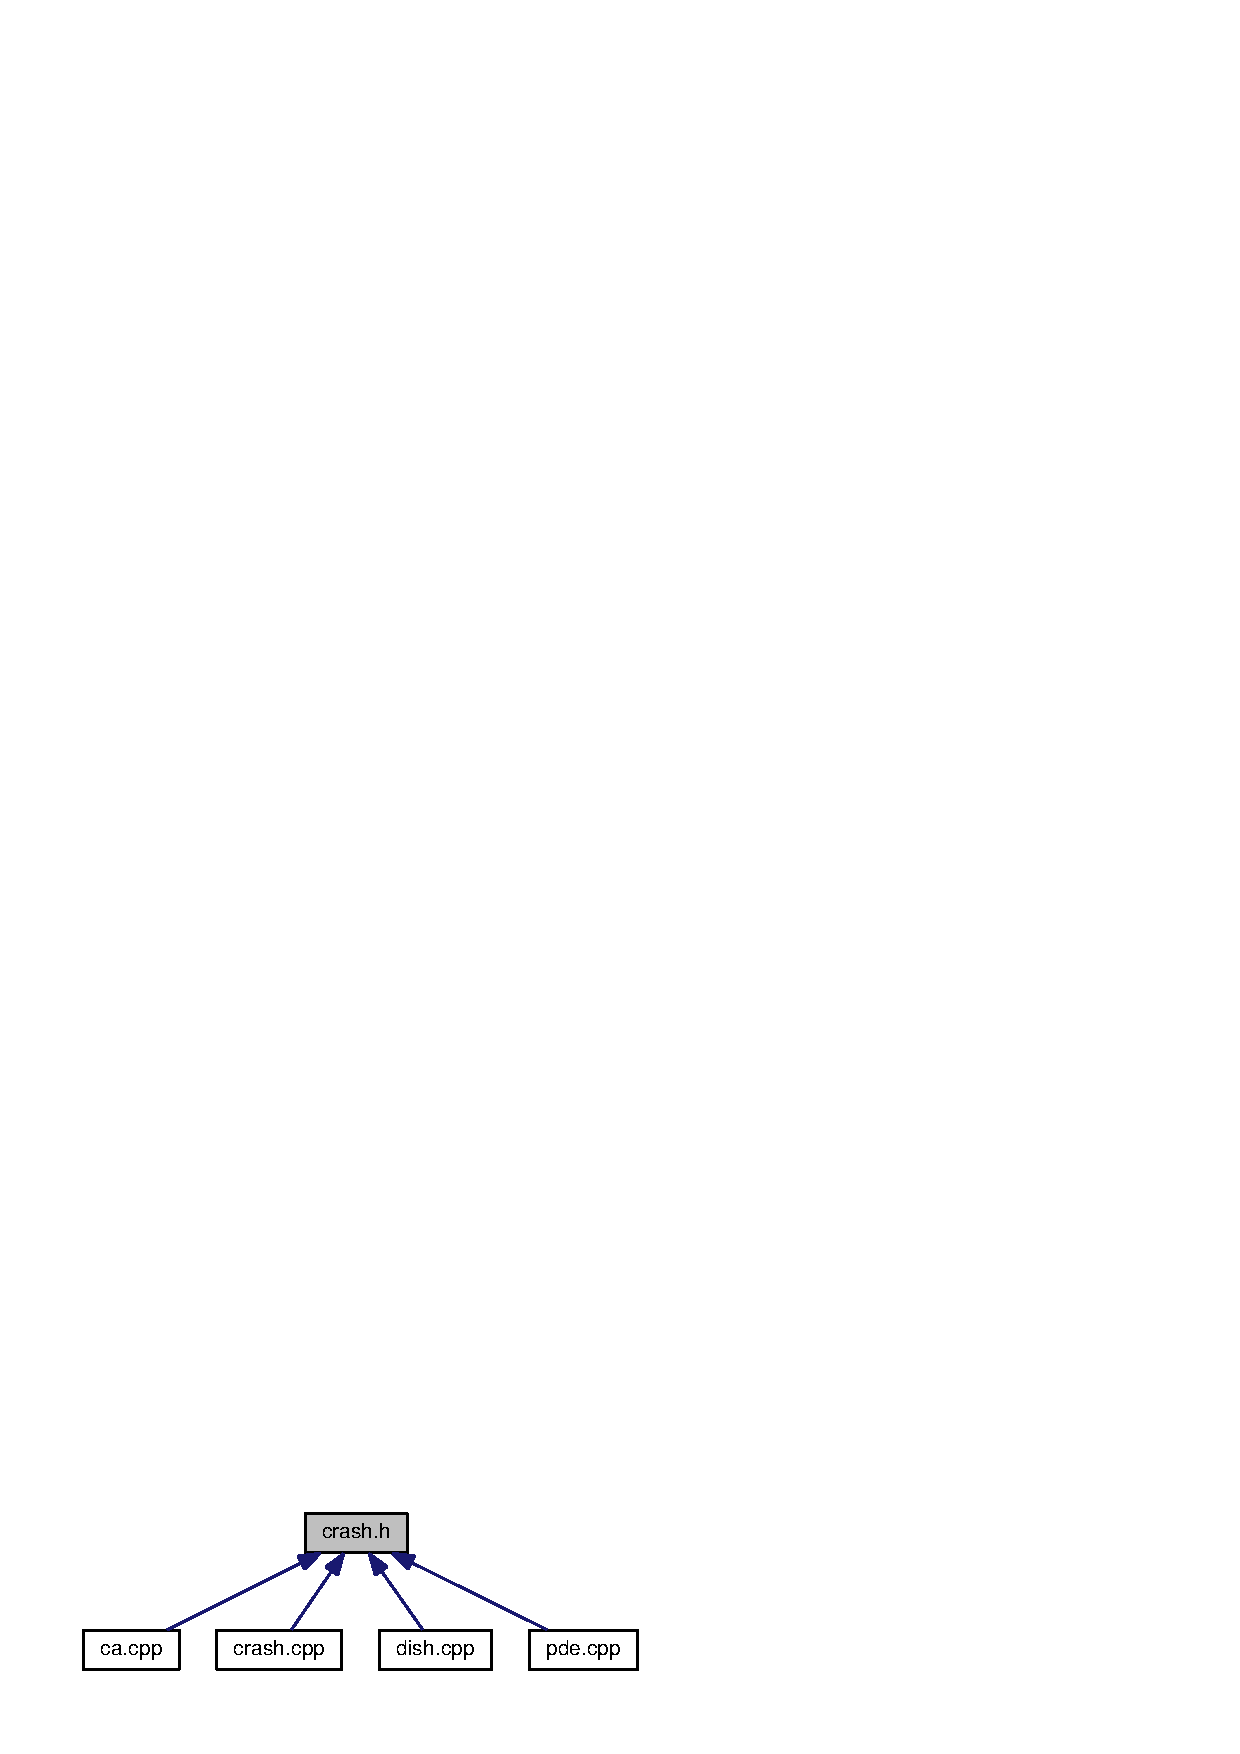
\includegraphics[width=310pt]{crash_8h__dep__incl}
\end{center}
\end{figure}
\subsection*{Functions}
\begin{DoxyCompactItemize}
\item 
void {\bf Start\-S\-I\-G\-I\-N\-T\-Handling} ()
\item 
void {\bf Handle\-S\-I\-G\-I\-N\-T} (int dummy)
\item 
void {\bf Start\-S\-I\-G\-S\-E\-G\-V\-Handling} ()
\item 
void {\bf Handle\-S\-I\-G\-S\-E\-G\-V} (int dummy)
\item 
void {\bf Nice\-Message} ()
\item 
void {\bf Memory\-Warning} (void)
\item 
void {\bf Crash} (char $\ast$message)
\end{DoxyCompactItemize}


\subsection{Function Documentation}
\index{crash.\-h@{crash.\-h}!Crash@{Crash}}
\index{Crash@{Crash}!crash.h@{crash.\-h}}
\subsubsection[{Crash}]{\setlength{\rightskip}{0pt plus 5cm}void Crash (
\begin{DoxyParamCaption}
\item[{char $\ast$}]{message}
\end{DoxyParamCaption}
)}\label{crash_8h_aa1a68e59048ea7e4b1e8ec147425715f}


Referenced by Handle\-S\-I\-G\-I\-N\-T(), Handle\-S\-I\-G\-S\-E\-G\-V(), and Memory\-Warning().

\index{crash.\-h@{crash.\-h}!Handle\-S\-I\-G\-I\-N\-T@{Handle\-S\-I\-G\-I\-N\-T}}
\index{Handle\-S\-I\-G\-I\-N\-T@{Handle\-S\-I\-G\-I\-N\-T}!crash.h@{crash.\-h}}
\subsubsection[{Handle\-S\-I\-G\-I\-N\-T}]{\setlength{\rightskip}{0pt plus 5cm}void Handle\-S\-I\-G\-I\-N\-T (
\begin{DoxyParamCaption}
\item[{int}]{dummy}
\end{DoxyParamCaption}
)}\label{crash_8h_a9204dc74d558cf88808a07563c0720e7}


References Crash().



Referenced by Start\-S\-I\-G\-I\-N\-T\-Handling().

\index{crash.\-h@{crash.\-h}!Handle\-S\-I\-G\-S\-E\-G\-V@{Handle\-S\-I\-G\-S\-E\-G\-V}}
\index{Handle\-S\-I\-G\-S\-E\-G\-V@{Handle\-S\-I\-G\-S\-E\-G\-V}!crash.h@{crash.\-h}}
\subsubsection[{Handle\-S\-I\-G\-S\-E\-G\-V}]{\setlength{\rightskip}{0pt plus 5cm}void Handle\-S\-I\-G\-S\-E\-G\-V (
\begin{DoxyParamCaption}
\item[{int}]{dummy}
\end{DoxyParamCaption}
)}\label{crash_8h_a8b93c1fe9e113ae0de5b3fec7d9c96c3}


References Crash().



Referenced by Start\-S\-I\-G\-S\-E\-G\-V\-Handling().

\index{crash.\-h@{crash.\-h}!Memory\-Warning@{Memory\-Warning}}
\index{Memory\-Warning@{Memory\-Warning}!crash.h@{crash.\-h}}
\subsubsection[{Memory\-Warning}]{\setlength{\rightskip}{0pt plus 5cm}void Memory\-Warning (
\begin{DoxyParamCaption}
\item[{void}]{}
\end{DoxyParamCaption}
)}\label{crash_8h_aa7a71c80db8162c3dbcf8d4343abd3eb}


References Crash().



Referenced by Cellular\-Potts\-::\-Allocate\-Sigma(), P\-D\-E\-::\-Allocate\-Sigma(), Cellular\-Potts\-::\-Find\-Cell\-Directions(), Cellular\-Potts\-::\-Grow\-In\-Cells(), Cellular\-Potts\-::\-Read\-Zygote\-Picture(), and Cellular\-Potts\-::\-Search\-Nand\-Plot().

\index{crash.\-h@{crash.\-h}!Nice\-Message@{Nice\-Message}}
\index{Nice\-Message@{Nice\-Message}!crash.h@{crash.\-h}}
\subsubsection[{Nice\-Message}]{\setlength{\rightskip}{0pt plus 5cm}void Nice\-Message (
\begin{DoxyParamCaption}
{}
\end{DoxyParamCaption}
)}\label{crash_8h_a12d2cdb667c7fc02143f95f6caf5b299}


Referenced by Start\-S\-I\-G\-I\-N\-T\-Handling().

\index{crash.\-h@{crash.\-h}!Start\-S\-I\-G\-I\-N\-T\-Handling@{Start\-S\-I\-G\-I\-N\-T\-Handling}}
\index{Start\-S\-I\-G\-I\-N\-T\-Handling@{Start\-S\-I\-G\-I\-N\-T\-Handling}!crash.h@{crash.\-h}}
\subsubsection[{Start\-S\-I\-G\-I\-N\-T\-Handling}]{\setlength{\rightskip}{0pt plus 5cm}void Start\-S\-I\-G\-I\-N\-T\-Handling (
\begin{DoxyParamCaption}
{}
\end{DoxyParamCaption}
)}\label{crash_8h_a8f556bfd09e856fb90fcd0d8569102ac}


References Handle\-S\-I\-G\-I\-N\-T(), and Nice\-Message().

\index{crash.\-h@{crash.\-h}!Start\-S\-I\-G\-S\-E\-G\-V\-Handling@{Start\-S\-I\-G\-S\-E\-G\-V\-Handling}}
\index{Start\-S\-I\-G\-S\-E\-G\-V\-Handling@{Start\-S\-I\-G\-S\-E\-G\-V\-Handling}!crash.h@{crash.\-h}}
\subsubsection[{Start\-S\-I\-G\-S\-E\-G\-V\-Handling}]{\setlength{\rightskip}{0pt plus 5cm}void Start\-S\-I\-G\-S\-E\-G\-V\-Handling (
\begin{DoxyParamCaption}
{}
\end{DoxyParamCaption}
)}\label{crash_8h_ad8a6bbf5a9b18ae6a4f66ae84d16d48a}


References Handle\-S\-I\-G\-S\-E\-G\-V().


\section{dish.\-cpp File Reference}
\label{dish_8cpp}\index{dish.\-cpp@{dish.\-cpp}}
{\ttfamily \#include $<$vector$>$}\\*
{\ttfamily \#include $<$list$>$}\\*
{\ttfamily \#include $<$algorithm$>$}\\*
{\ttfamily \#include $<$fstream$>$}\\*
{\ttfamily \#include $<$string.\-h$>$}\\*
{\ttfamily \#include $<$errno.\-h$>$}\\*
{\ttfamily \#include $<$math.\-h$>$}\\*
{\ttfamily \#include \char`\"{}dish.\-h\char`\"{}}\\*
{\ttfamily \#include \char`\"{}sticky.\-h\char`\"{}}\\*
{\ttfamily \#include \char`\"{}parameter.\-h\char`\"{}}\\*
{\ttfamily \#include \char`\"{}info.\-h\char`\"{}}\\*
{\ttfamily \#include \char`\"{}crash.\-h\char`\"{}}\\*
{\ttfamily \#include \char`\"{}pde.\-h\char`\"{}}\\*
Include dependency graph for dish.\-cpp\-:
\nopagebreak
\begin{figure}[H]
\begin{center}
\leavevmode
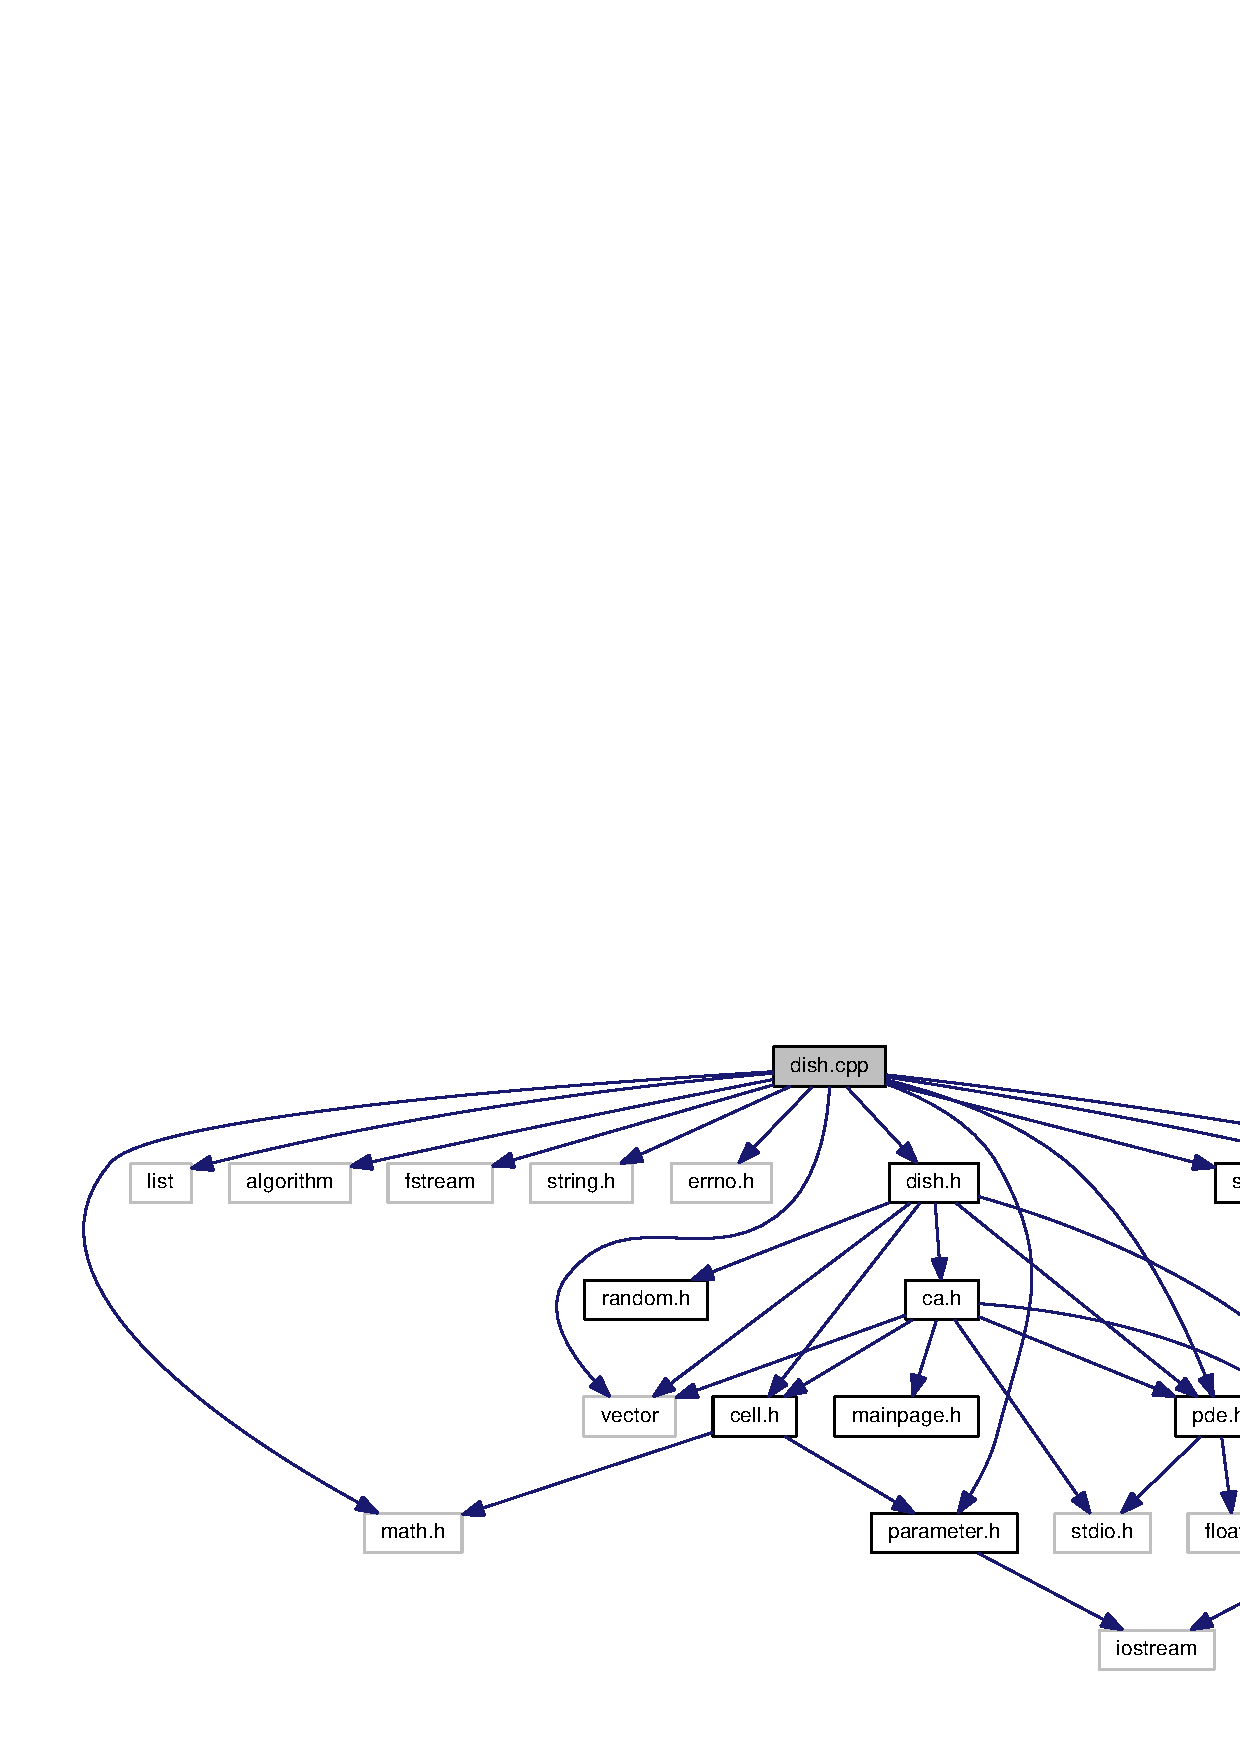
\includegraphics[width=350pt]{dish_8cpp__incl}
\end{center}
\end{figure}
\subsection*{Macros}
\begin{DoxyCompactItemize}
\item 
\#define {\bf E\-X\-T\-E\-R\-N\-A\-L\-\_\-\-O\-F\-F}
\end{DoxyCompactItemize}
\subsection*{Variables}
\begin{DoxyCompactItemize}
\item 
{\bf Parameter} {\bf par}
\end{DoxyCompactItemize}


\subsection{Macro Definition Documentation}
\index{dish.\-cpp@{dish.\-cpp}!E\-X\-T\-E\-R\-N\-A\-L\-\_\-\-O\-F\-F@{E\-X\-T\-E\-R\-N\-A\-L\-\_\-\-O\-F\-F}}
\index{E\-X\-T\-E\-R\-N\-A\-L\-\_\-\-O\-F\-F@{E\-X\-T\-E\-R\-N\-A\-L\-\_\-\-O\-F\-F}!dish.cpp@{dish.\-cpp}}
\subsubsection[{E\-X\-T\-E\-R\-N\-A\-L\-\_\-\-O\-F\-F}]{\setlength{\rightskip}{0pt plus 5cm}\#define E\-X\-T\-E\-R\-N\-A\-L\-\_\-\-O\-F\-F}\label{dish_8cpp_a3c638035d71663ea96aecfeea6817aa5}


\subsection{Variable Documentation}
\index{dish.\-cpp@{dish.\-cpp}!par@{par}}
\index{par@{par}!dish.cpp@{dish.\-cpp}}
\subsubsection[{par}]{\setlength{\rightskip}{0pt plus 5cm}{\bf Parameter} par}\label{dish_8cpp_aa11a52593a908c20a7259a3e72c0b348}

\section{dish.\-h File Reference}
\label{dish_8h}\index{dish.\-h@{dish.\-h}}
{\ttfamily \#include $<$vector$>$}\\*
{\ttfamily \#include \char`\"{}graph.\-h\char`\"{}}\\*
{\ttfamily \#include \char`\"{}random.\-h\char`\"{}}\\*
{\ttfamily \#include \char`\"{}pde.\-h\char`\"{}}\\*
{\ttfamily \#include \char`\"{}cell.\-h\char`\"{}}\\*
{\ttfamily \#include \char`\"{}ca.\-h\char`\"{}}\\*
Include dependency graph for dish.\-h\-:
\nopagebreak
\begin{figure}[H]
\begin{center}
\leavevmode
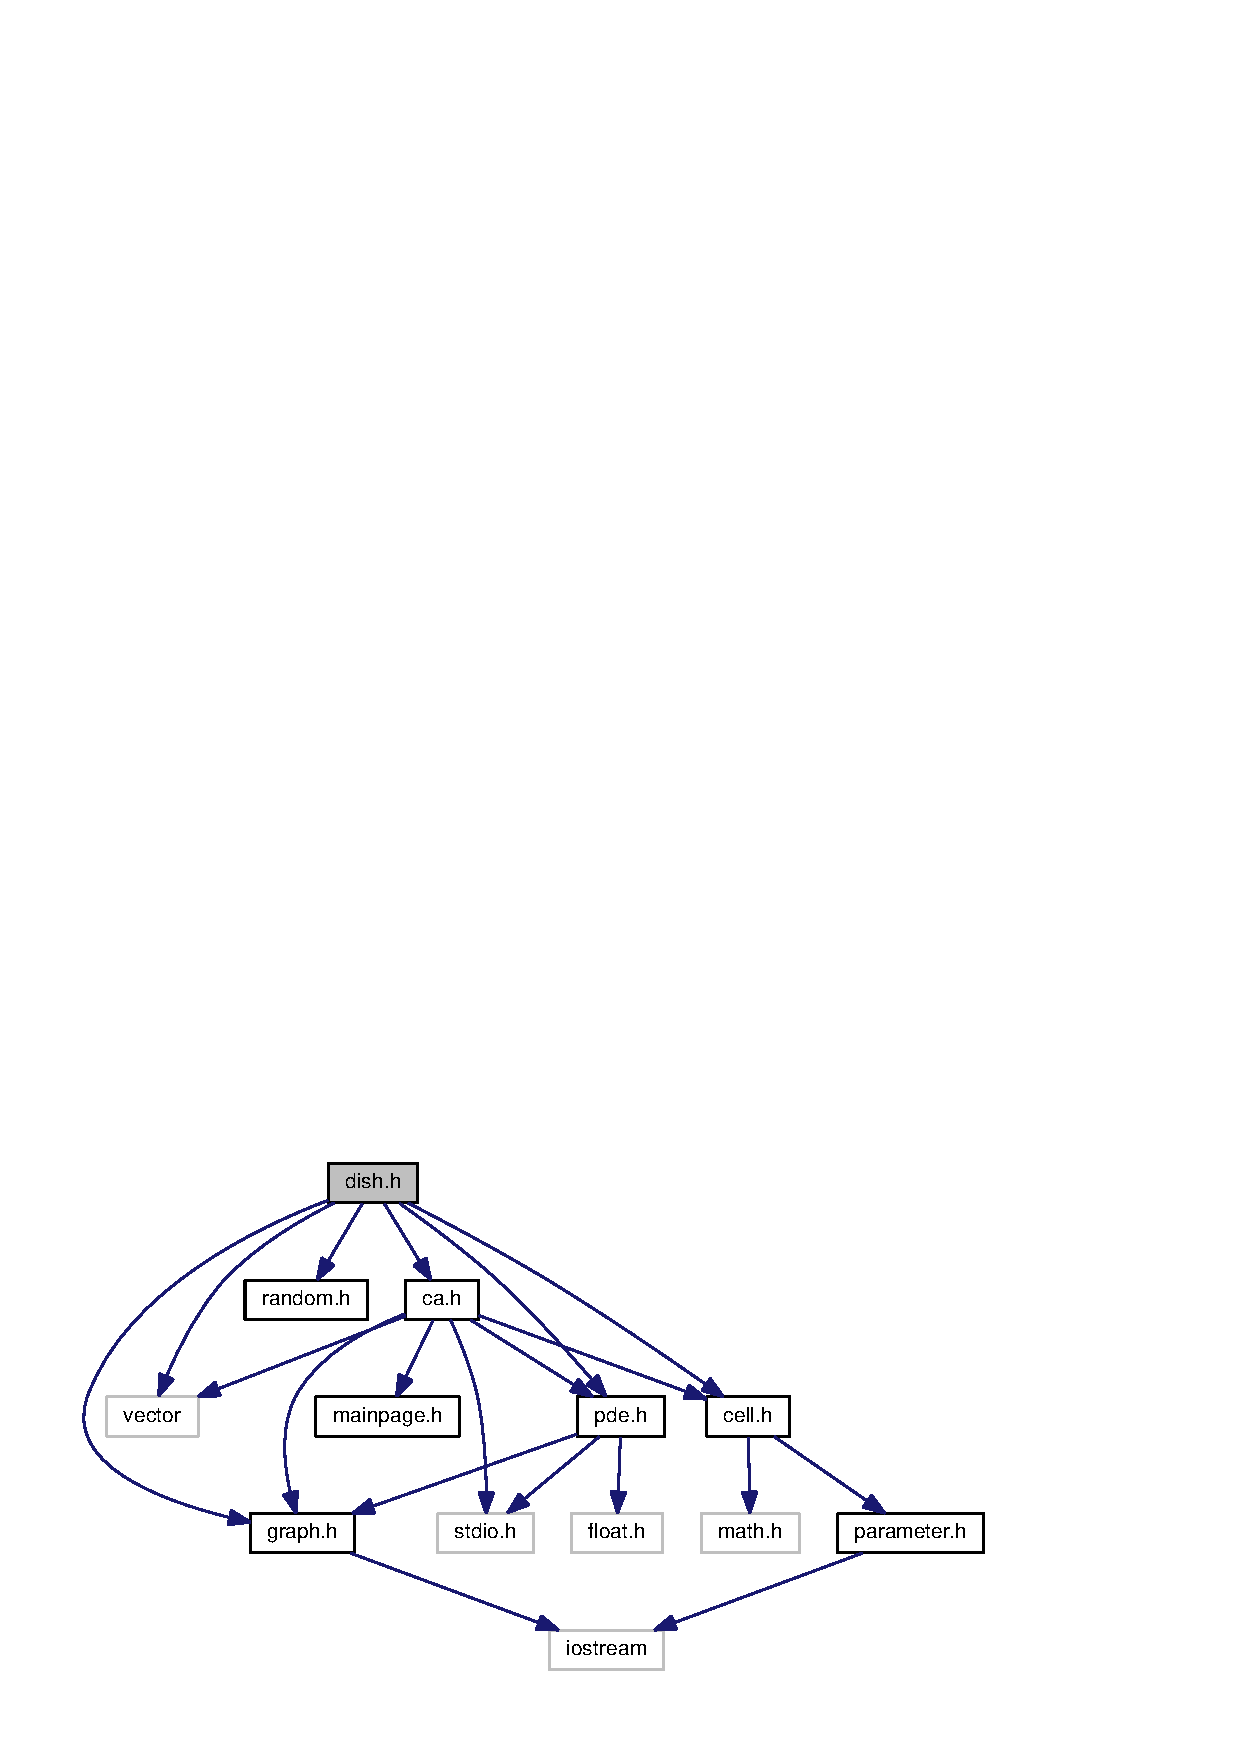
\includegraphics[width=350pt]{dish_8h__incl}
\end{center}
\end{figure}
This graph shows which files directly or indirectly include this file\-:
\nopagebreak
\begin{figure}[H]
\begin{center}
\leavevmode
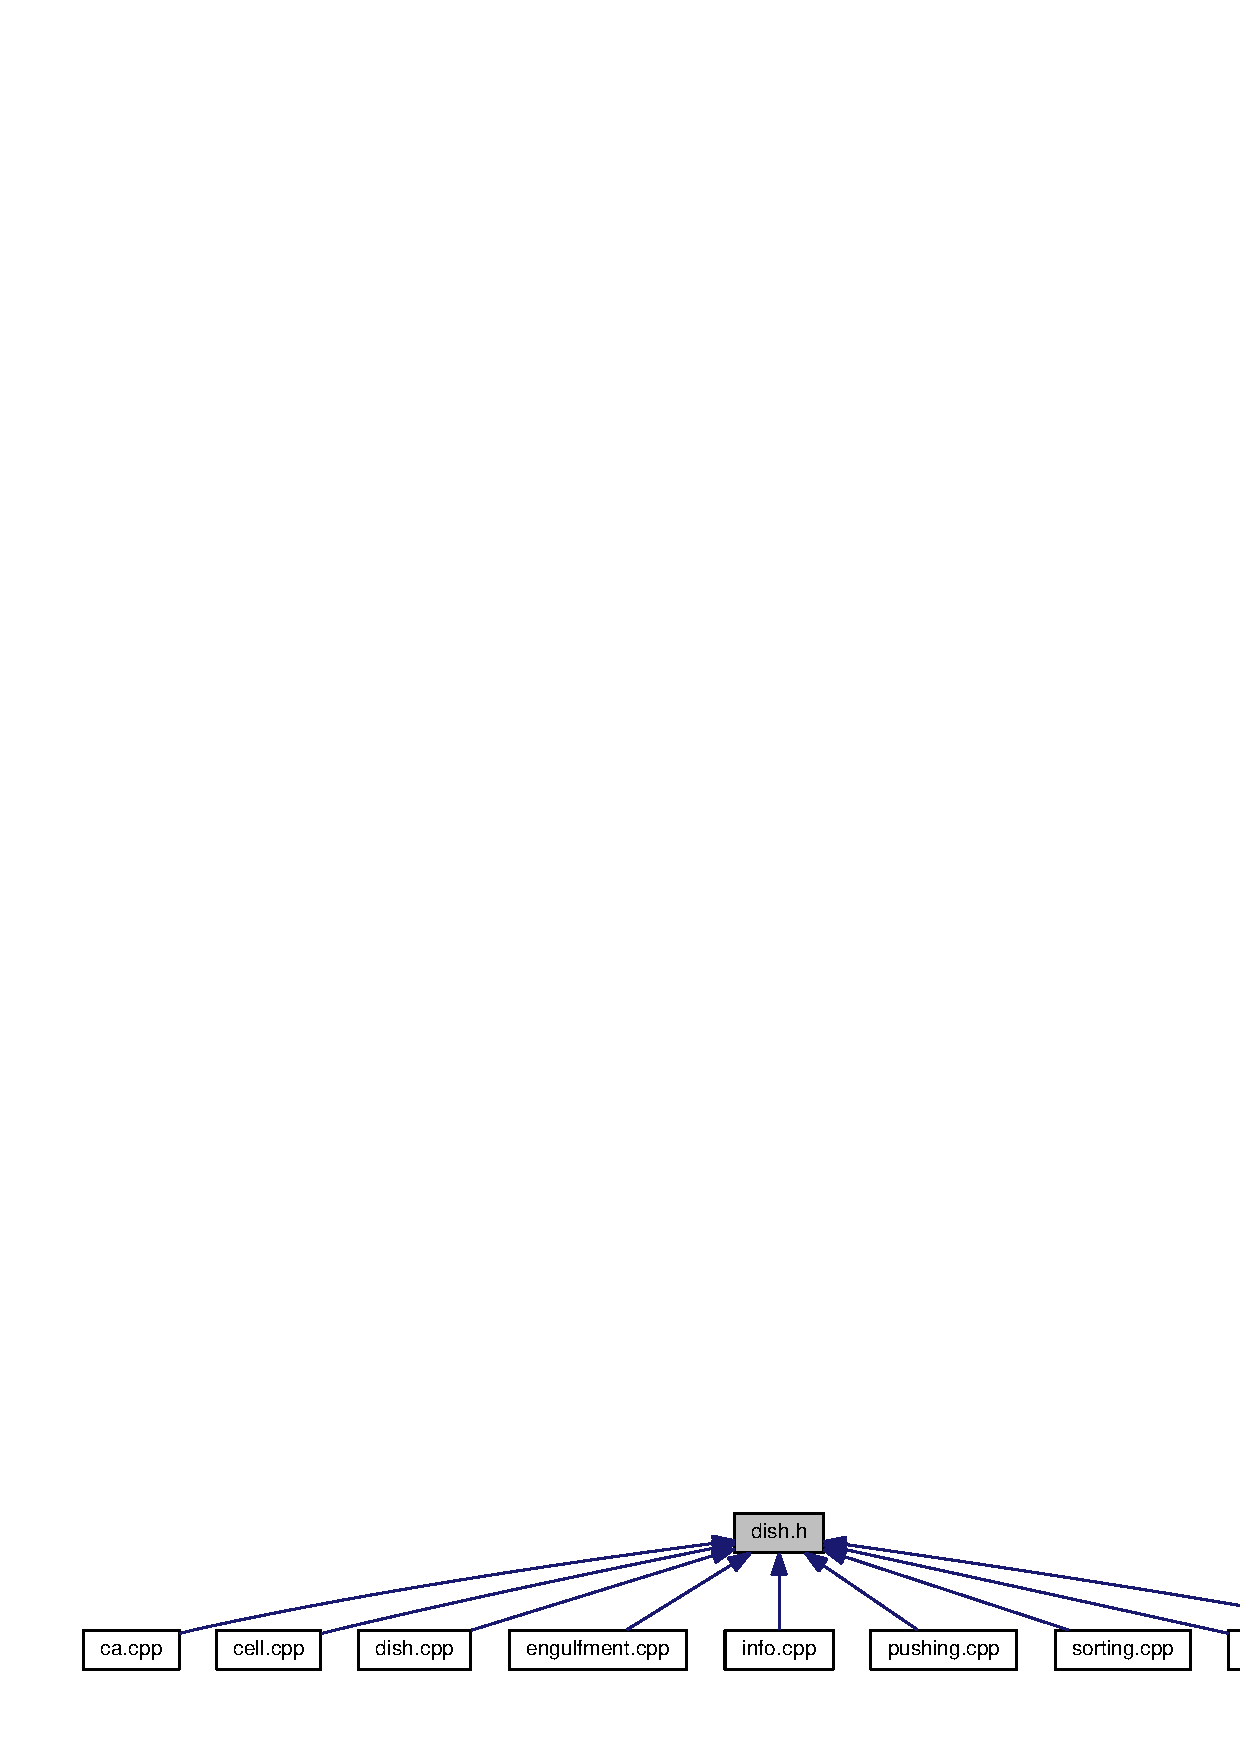
\includegraphics[width=350pt]{dish_8h__dep__incl}
\end{center}
\end{figure}
\subsection*{Classes}
\begin{DoxyCompactItemize}
\item 
class {\bf Dish}
\begin{DoxyCompactList}\small\item\em The virtual Petri dish. \end{DoxyCompactList}\end{DoxyCompactItemize}
\subsection*{Namespaces}
\begin{DoxyCompactItemize}
\item 
{\bf Colour\-Mode}
\end{DoxyCompactItemize}
\subsection*{Macros}
\begin{DoxyCompactItemize}
\item 
\#define {\bf I\-N\-I\-T}~void {\bf Dish\-::\-Init}(void)
\end{DoxyCompactItemize}
\subsection*{Enumerations}
\begin{DoxyCompactItemize}
\item 
enum \{ {\bf Colour\-Mode\-::\-State}, 
{\bf Colour\-Mode\-::\-Cell\-Type}, 
{\bf Colour\-Mode\-::\-Sigma}, 
{\bf Colour\-Mode\-::\-Auxilliary}
 \}
\end{DoxyCompactItemize}


\subsection{Macro Definition Documentation}
\index{dish.\-h@{dish.\-h}!I\-N\-I\-T@{I\-N\-I\-T}}
\index{I\-N\-I\-T@{I\-N\-I\-T}!dish.h@{dish.\-h}}
\subsubsection[{I\-N\-I\-T}]{\setlength{\rightskip}{0pt plus 5cm}\#define I\-N\-I\-T~void {\bf Dish\-::\-Init}(void)}\label{dish_8h_ab5889105dcd019008c9448dff61323f6}

\section{engulfment.\-cpp File Reference}
\label{engulfment_8cpp}\index{engulfment.\-cpp@{engulfment.\-cpp}}
{\ttfamily \#include $<$stdio.\-h$>$}\\*
{\ttfamily \#include $<$malloc.\-h$>$}\\*
{\ttfamily \#include $<$iostream$>$}\\*
{\ttfamily \#include $<$cstdlib$>$}\\*
{\ttfamily \#include $<$algorithm$>$}\\*
{\ttfamily \#include $<$fstream$>$}\\*
{\ttfamily \#include $<$math.\-h$>$}\\*
{\ttfamily \#include \char`\"{}dish.\-h\char`\"{}}\\*
{\ttfamily \#include \char`\"{}random.\-h\char`\"{}}\\*
{\ttfamily \#include \char`\"{}cell.\-h\char`\"{}}\\*
{\ttfamily \#include \char`\"{}info.\-h\char`\"{}}\\*
{\ttfamily \#include \char`\"{}parameter.\-h\char`\"{}}\\*
{\ttfamily \#include \char`\"{}morphometry.\-h\char`\"{}}\\*
{\ttfamily \#include \char`\"{}sqr.\-h\char`\"{}}\\*
{\ttfamily \#include \char`\"{}x11graph.\-h\char`\"{}}\\*
Include dependency graph for engulfment.\-cpp\-:
\nopagebreak
\begin{figure}[H]
\begin{center}
\leavevmode
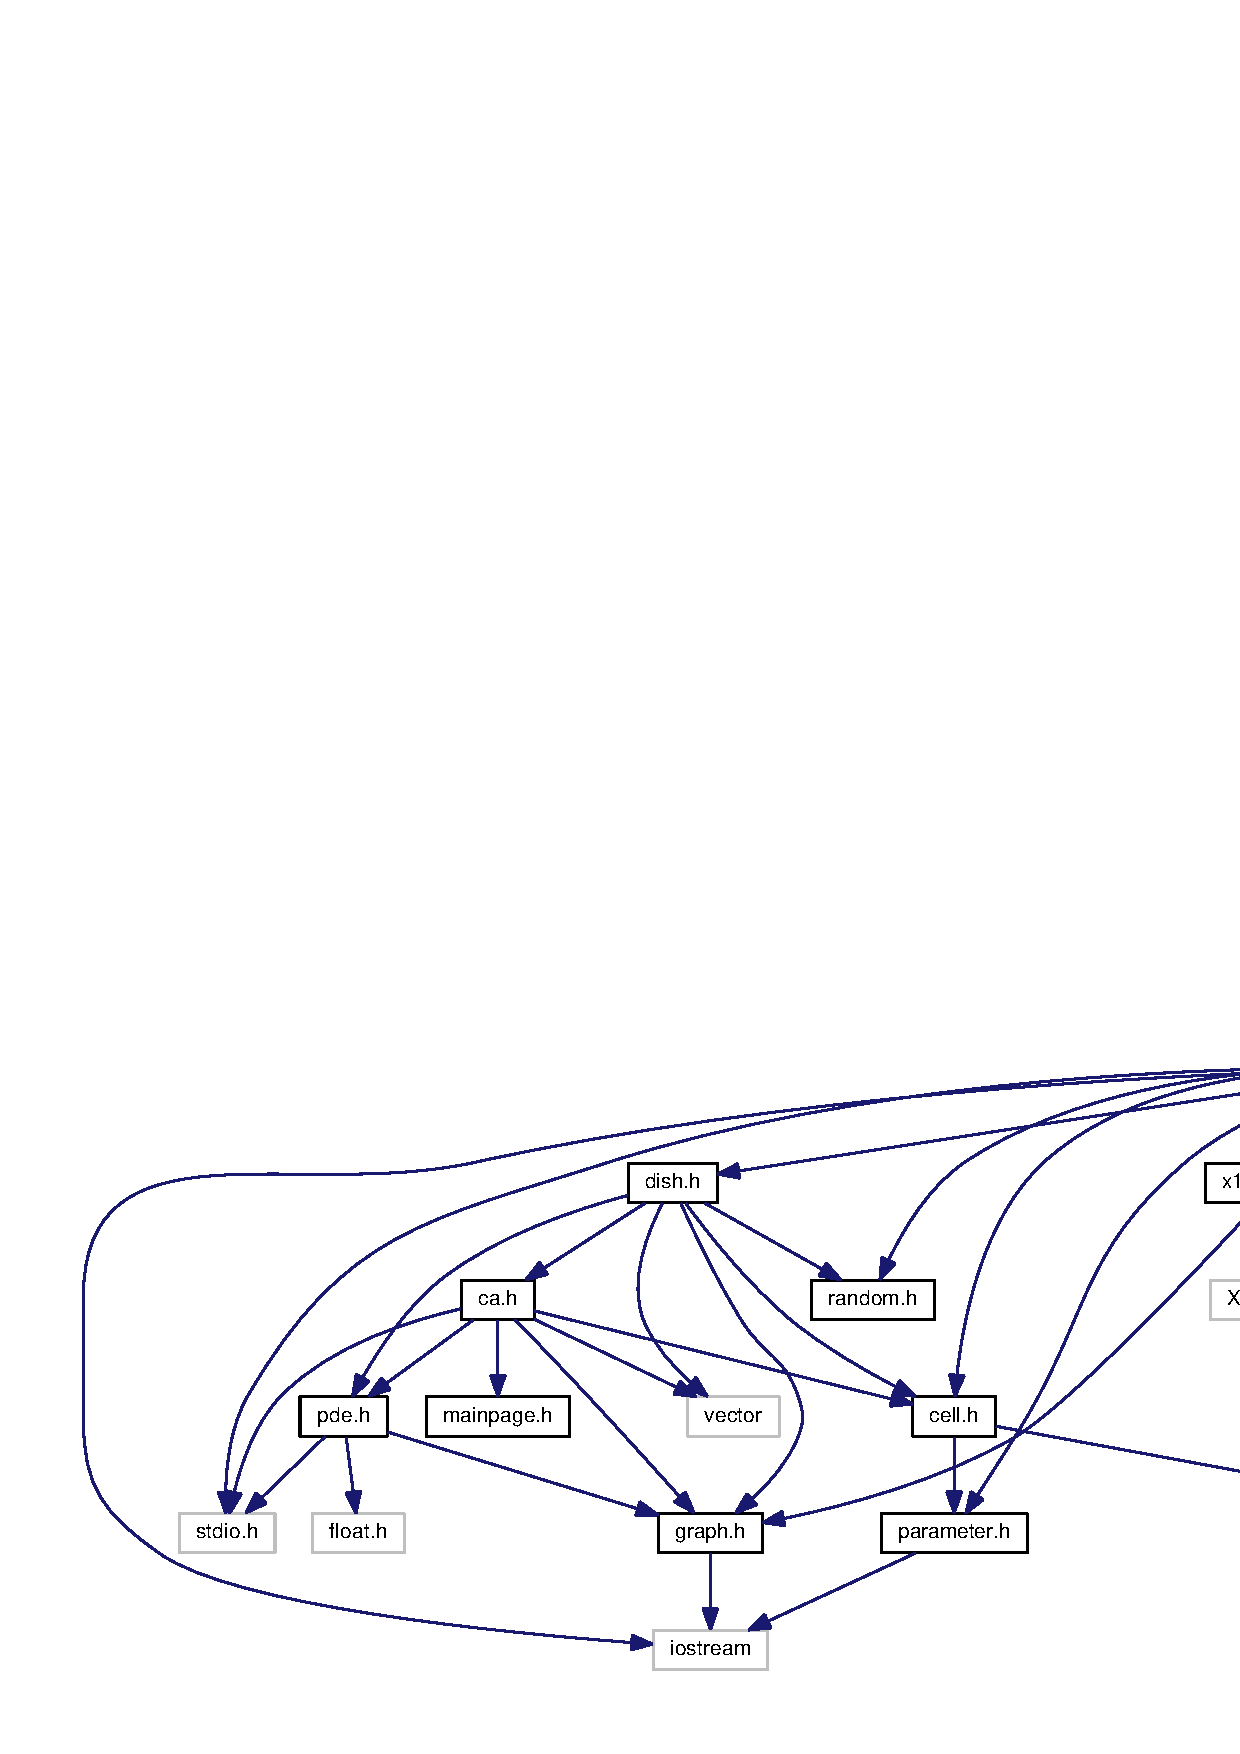
\includegraphics[width=350pt]{engulfment_8cpp__incl}
\end{center}
\end{figure}

\section{graph.\-h File Reference}
\label{graph_8h}\index{graph.\-h@{graph.\-h}}
{\ttfamily \#include $<$iostream$>$}\\*
Include dependency graph for graph.\-h\-:
\nopagebreak
\begin{figure}[H]
\begin{center}
\leavevmode
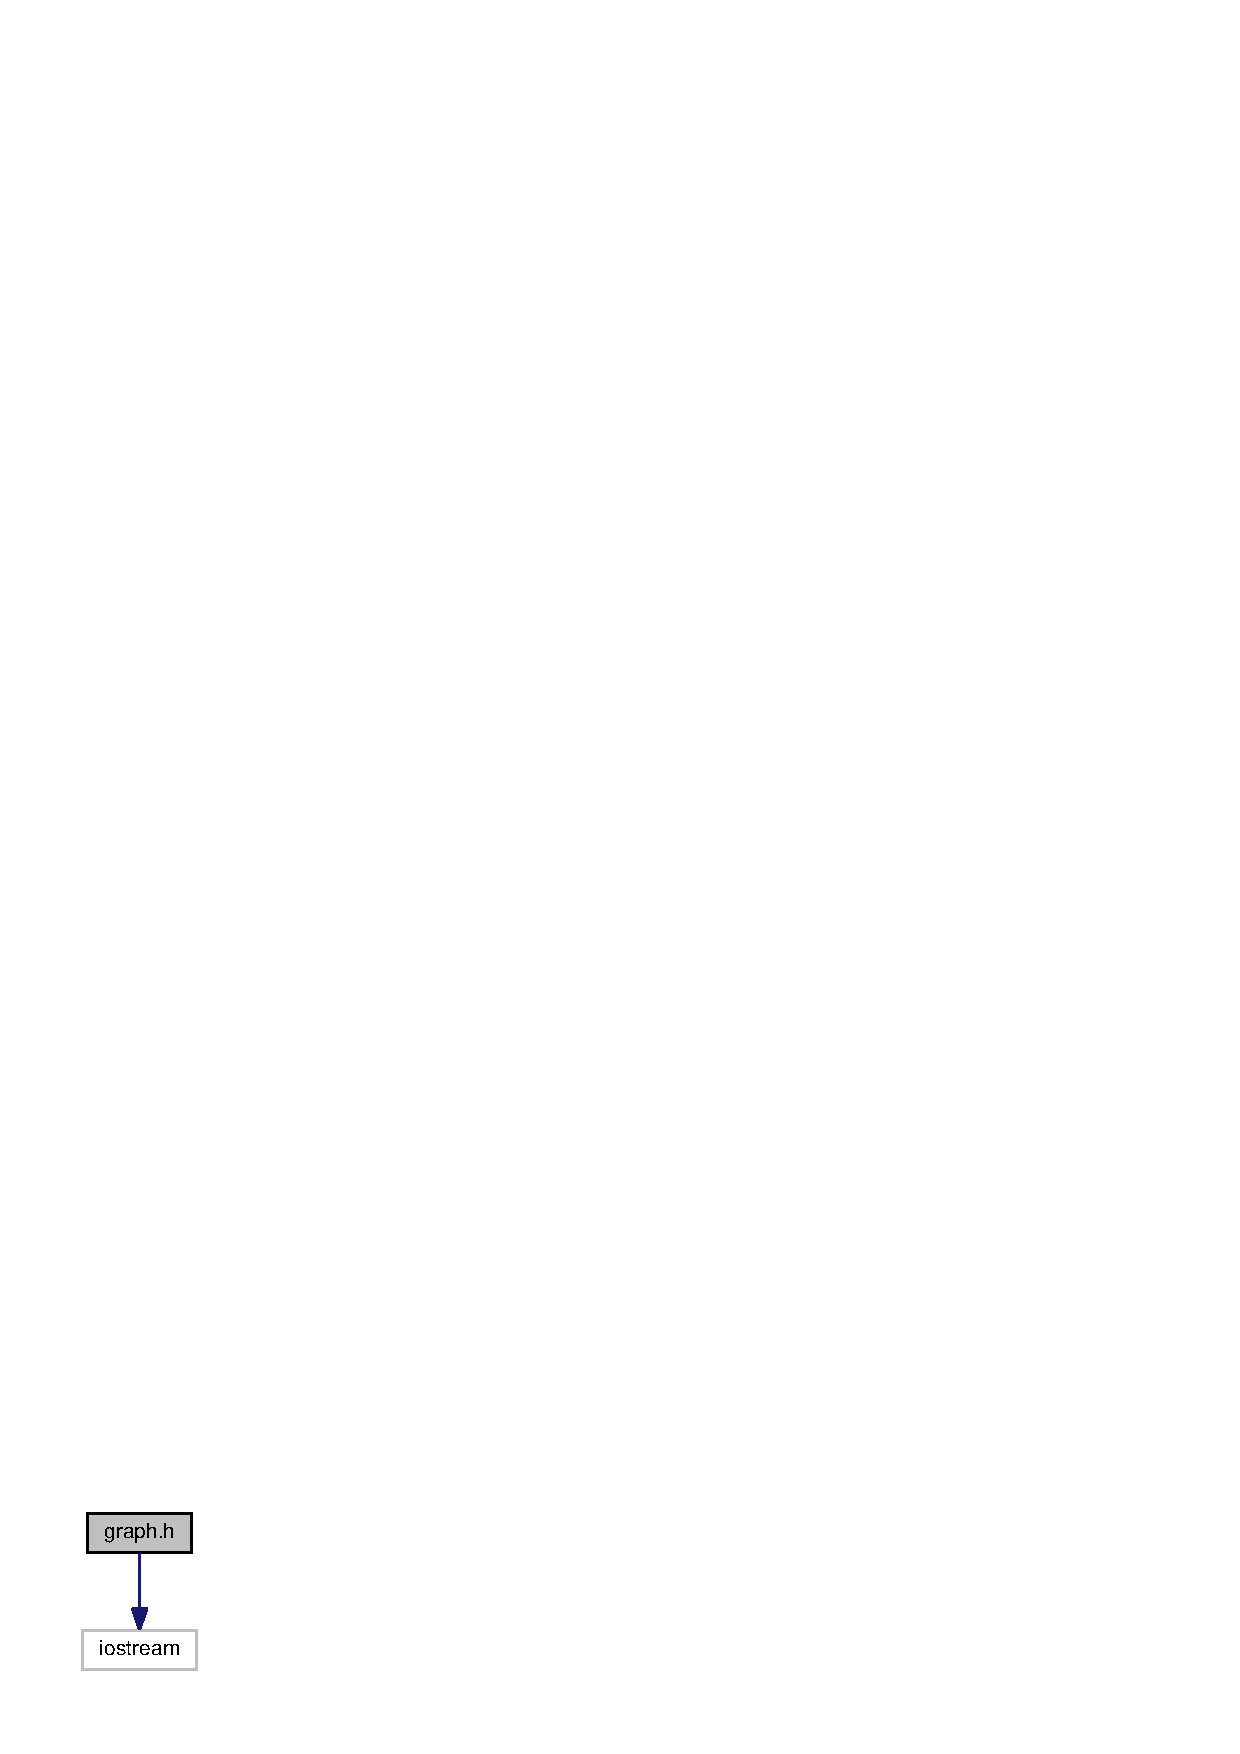
\includegraphics[width=98pt]{graph_8h__incl}
\end{center}
\end{figure}
This graph shows which files directly or indirectly include this file\-:
\nopagebreak
\begin{figure}[H]
\begin{center}
\leavevmode
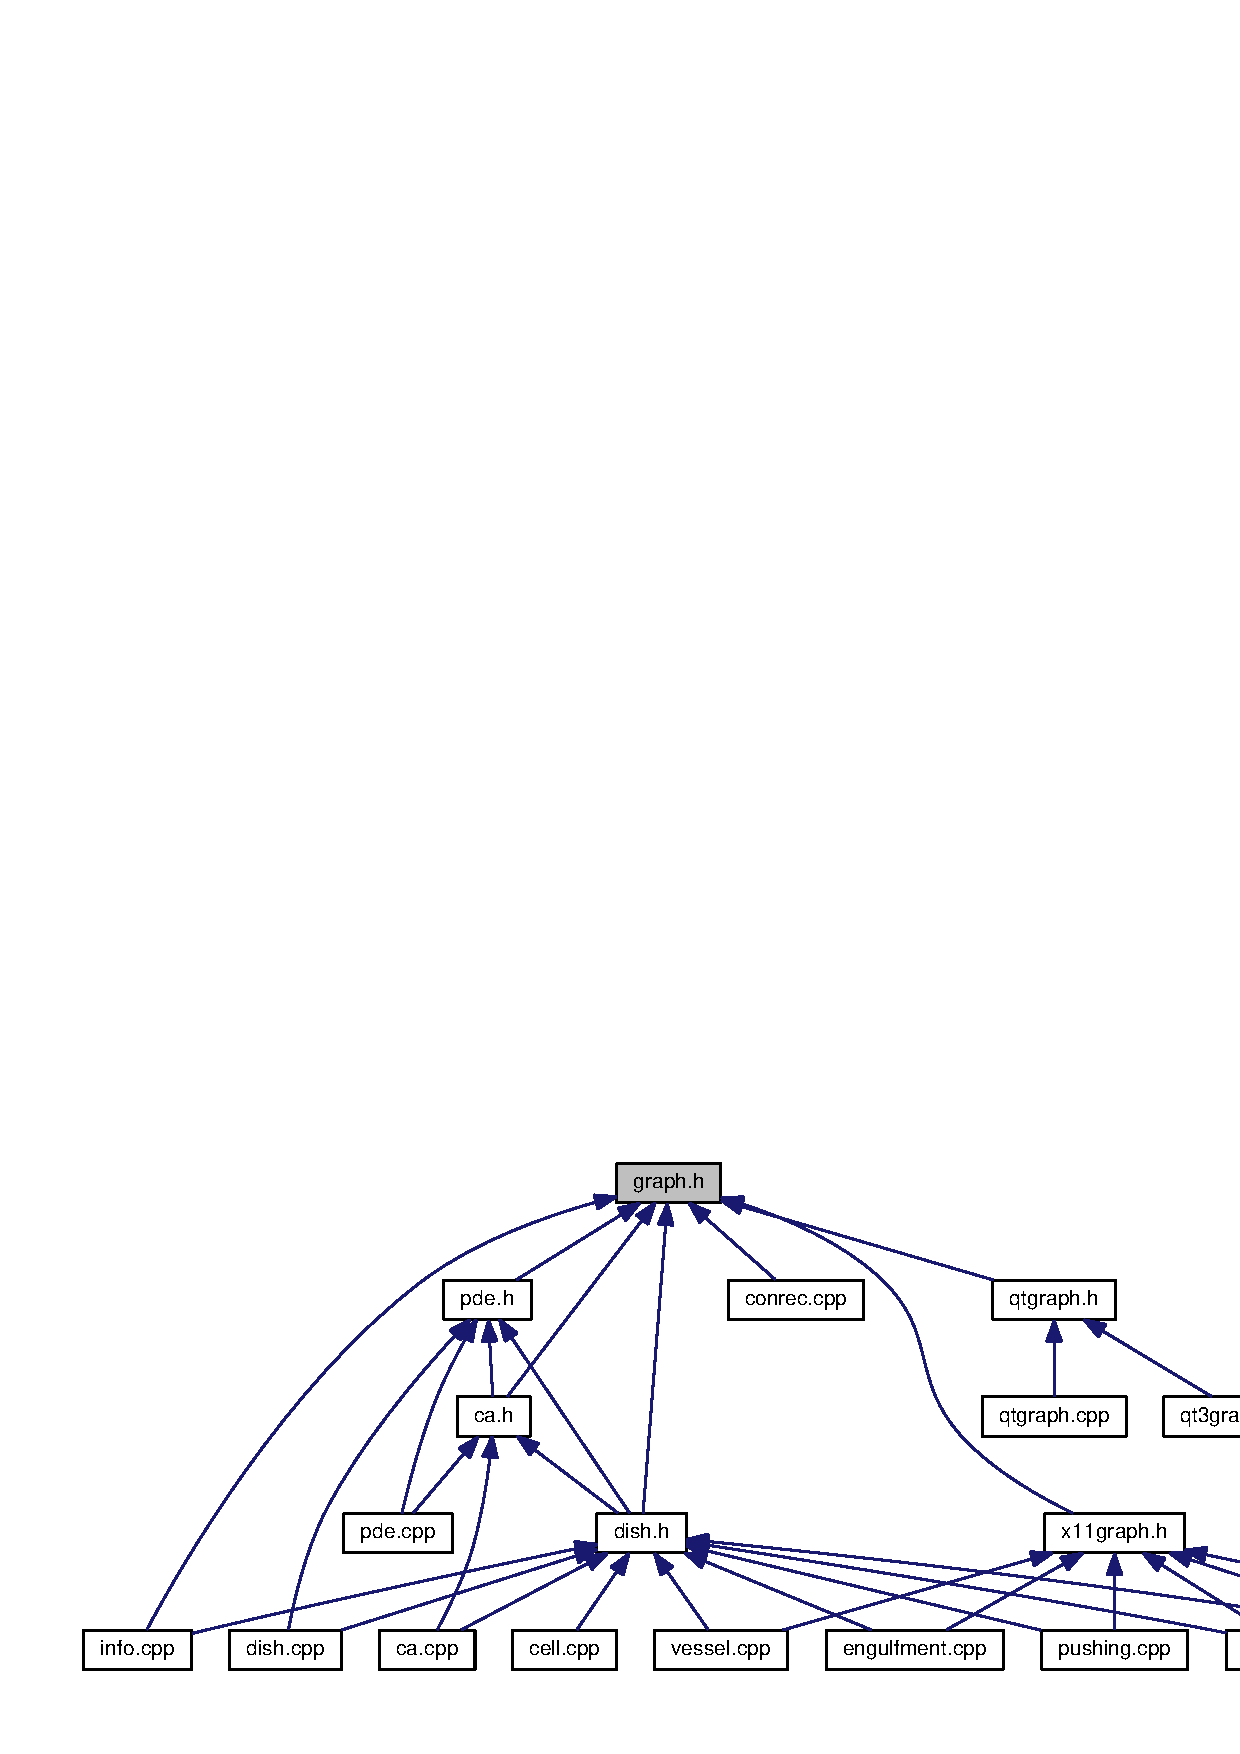
\includegraphics[width=350pt]{graph_8h__dep__incl}
\end{center}
\end{figure}
\subsection*{Classes}
\begin{DoxyCompactItemize}
\item 
class {\bf Graphics}
\begin{DoxyCompactList}\small\item\em A\-P\-I for \doxyref{Graphics}{p.}{classGraphics} windows. \end{DoxyCompactList}\end{DoxyCompactItemize}

\section{hull.\-cpp File Reference}
\label{hull_8cpp}\index{hull.\-cpp@{hull.\-cpp}}
{\ttfamily \#include \char`\"{}hull.\-h\char`\"{}}\\*
Include dependency graph for hull.\-cpp\-:
\nopagebreak
\begin{figure}[H]
\begin{center}
\leavevmode
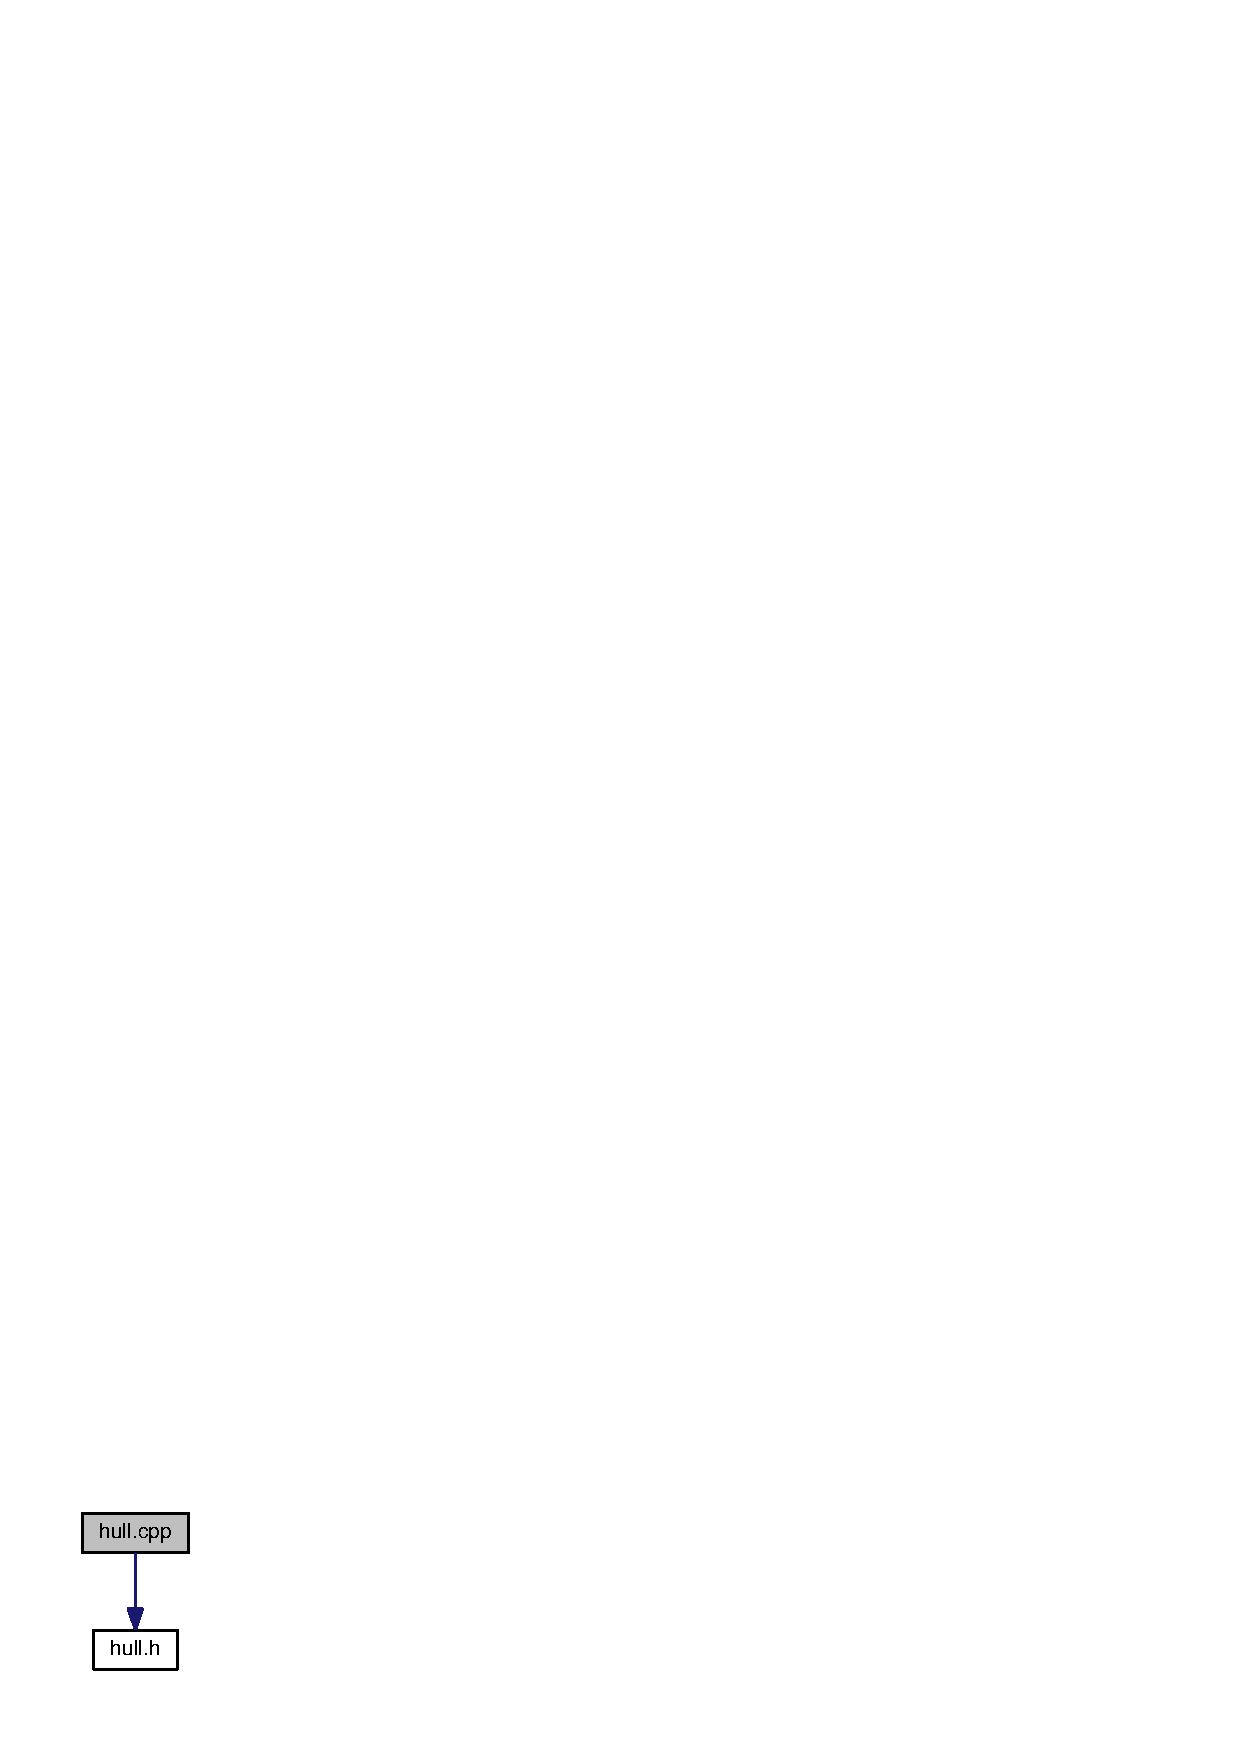
\includegraphics[width=94pt]{hull_8cpp__incl}
\end{center}
\end{figure}
\subsection*{Functions}
\begin{DoxyCompactItemize}
\item 
float {\bf is\-Left} ({\bf Point} P0, {\bf Point} P1, {\bf Point} P2)
\item 
int {\bf chain\-Hull\-\_\-2\-D} ({\bf Point} $\ast$P, int n, {\bf Point} $\ast$H)
\end{DoxyCompactItemize}


\subsection{Function Documentation}
\index{hull.\-cpp@{hull.\-cpp}!chain\-Hull\-\_\-2\-D@{chain\-Hull\-\_\-2\-D}}
\index{chain\-Hull\-\_\-2\-D@{chain\-Hull\-\_\-2\-D}!hull.cpp@{hull.\-cpp}}
\subsubsection[{chain\-Hull\-\_\-2\-D}]{\setlength{\rightskip}{0pt plus 5cm}int chain\-Hull\-\_\-2\-D (
\begin{DoxyParamCaption}
\item[{{\bf Point} $\ast$}]{P, }
\item[{int}]{n, }
\item[{{\bf Point} $\ast$}]{H}
\end{DoxyParamCaption}
)}\label{hull_8cpp_ad687868582cf5cc0fe52ae4d93f319cb}


References is\-Left(), and Point\-::x.



Referenced by Cellular\-Potts\-::\-Compactness(), and Cellular\-Potts\-::\-Draw\-Convex\-Hull().

\index{hull.\-cpp@{hull.\-cpp}!is\-Left@{is\-Left}}
\index{is\-Left@{is\-Left}!hull.cpp@{hull.\-cpp}}
\subsubsection[{is\-Left}]{\setlength{\rightskip}{0pt plus 5cm}float is\-Left (
\begin{DoxyParamCaption}
\item[{{\bf Point}}]{P0, }
\item[{{\bf Point}}]{P1, }
\item[{{\bf Point}}]{P2}
\end{DoxyParamCaption}
)\hspace{0.3cm}{\ttfamily [inline]}}\label{hull_8cpp_a1c45750c2758d03b8387378f556b4ee8}


References Point\-::x, and Point\-::y.



Referenced by chain\-Hull\-\_\-2\-D().


\section{hull.\-h File Reference}
\label{hull_8h}\index{hull.\-h@{hull.\-h}}
This graph shows which files directly or indirectly include this file\-:
\nopagebreak
\begin{figure}[H]
\begin{center}
\leavevmode
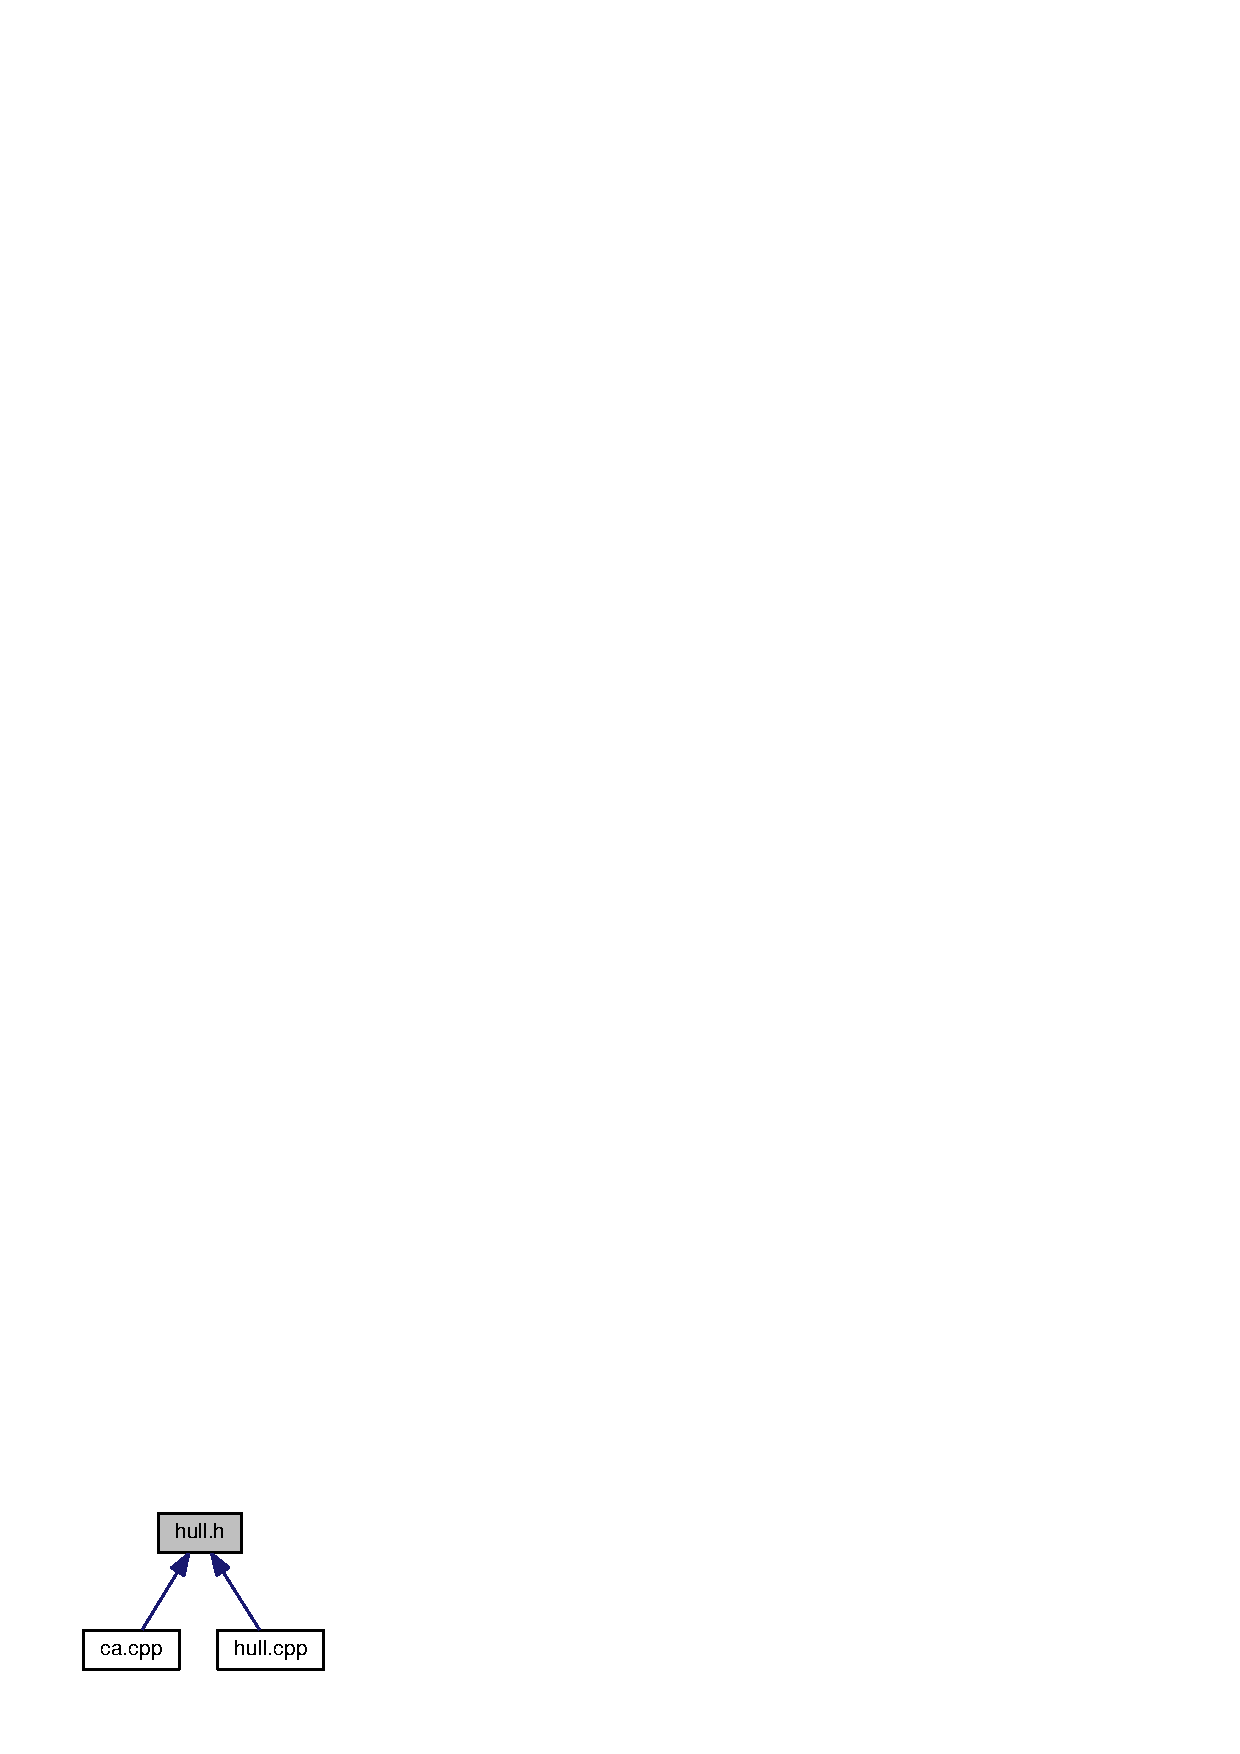
\includegraphics[width=159pt]{hull_8h__dep__incl}
\end{center}
\end{figure}
\subsection*{Classes}
\begin{DoxyCompactItemize}
\item 
class {\bf Point}
\end{DoxyCompactItemize}
\subsection*{Functions}
\begin{DoxyCompactItemize}
\item 
int {\bf chain\-Hull\-\_\-2\-D} ({\bf Point} $\ast$P, int n, {\bf Point} $\ast$H)
\end{DoxyCompactItemize}


\subsection{Function Documentation}
\index{hull.\-h@{hull.\-h}!chain\-Hull\-\_\-2\-D@{chain\-Hull\-\_\-2\-D}}
\index{chain\-Hull\-\_\-2\-D@{chain\-Hull\-\_\-2\-D}!hull.h@{hull.\-h}}
\subsubsection[{chain\-Hull\-\_\-2\-D}]{\setlength{\rightskip}{0pt plus 5cm}int chain\-Hull\-\_\-2\-D (
\begin{DoxyParamCaption}
\item[{{\bf Point} $\ast$}]{P, }
\item[{int}]{n, }
\item[{{\bf Point} $\ast$}]{H}
\end{DoxyParamCaption}
)}\label{hull_8h_ad687868582cf5cc0fe52ae4d93f319cb}


References is\-Left(), and Point\-::x.



Referenced by Cellular\-Potts\-::\-Compactness(), and Cellular\-Potts\-::\-Draw\-Convex\-Hull().


\section{info.\-cpp File Reference}
\label{info_8cpp}\index{info.\-cpp@{info.\-cpp}}
{\ttfamily \#include $<$iostream$>$}\\*
{\ttfamily \#include $<$math.\-h$>$}\\*
{\ttfamily \#include $<$fstream$>$}\\*
{\ttfamily \#include $<$malloc.\-h$>$}\\*
{\ttfamily \#include \char`\"{}dish.\-h\char`\"{}}\\*
{\ttfamily \#include \char`\"{}graph.\-h\char`\"{}}\\*
{\ttfamily \#include \char`\"{}info.\-h\char`\"{}}\\*
{\ttfamily \#include \char`\"{}parameter.\-h\char`\"{}}\\*
{\ttfamily \#include \char`\"{}misc.\-h\char`\"{}}\\*
{\ttfamily \#include \char`\"{}parse.\-h\char`\"{}}\\*
Include dependency graph for info.\-cpp\-:
\nopagebreak
\begin{figure}[H]
\begin{center}
\leavevmode
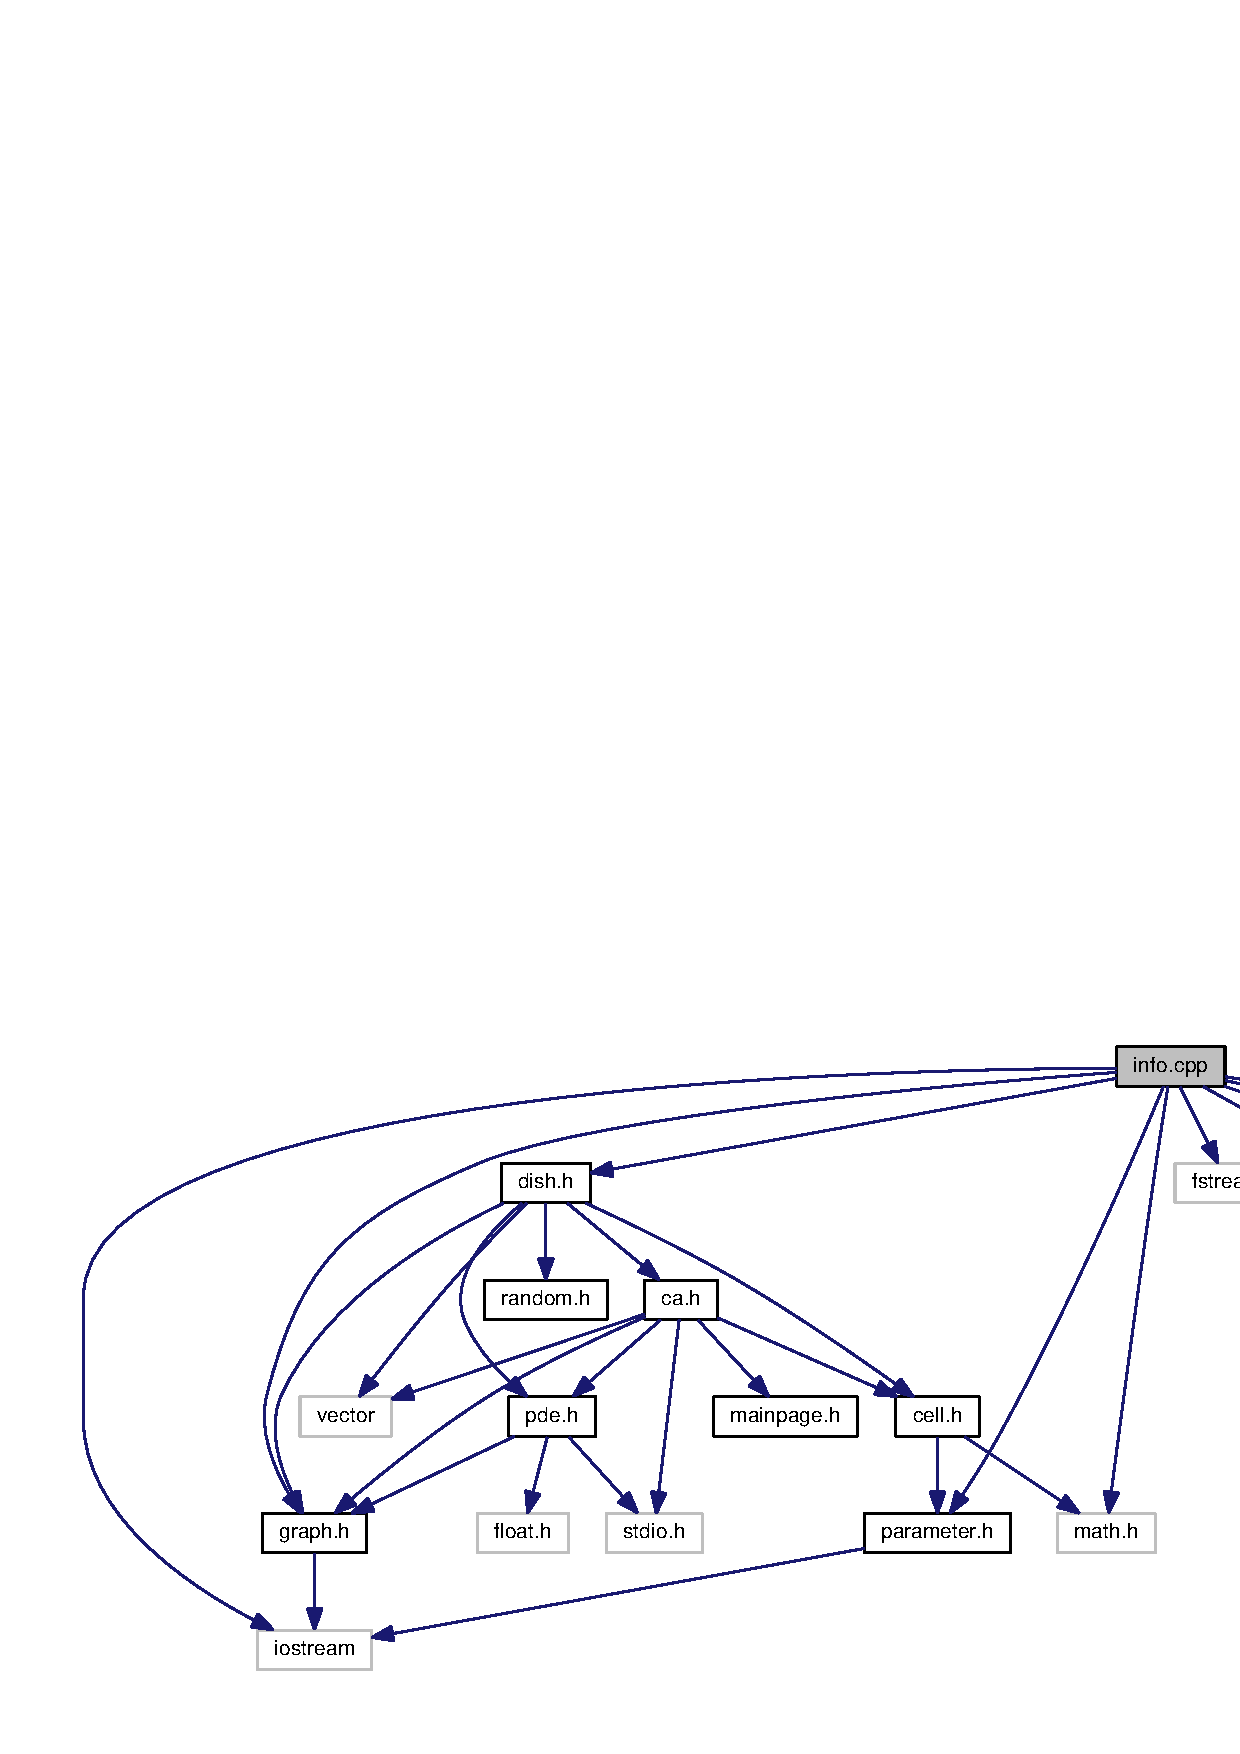
\includegraphics[width=350pt]{info_8cpp__incl}
\end{center}
\end{figure}
\subsection*{Variables}
\begin{DoxyCompactItemize}
\item 
{\bf Parameter} {\bf par}
\end{DoxyCompactItemize}


\subsection{Variable Documentation}
\index{info.\-cpp@{info.\-cpp}!par@{par}}
\index{par@{par}!info.cpp@{info.\-cpp}}
\subsubsection[{par}]{\setlength{\rightskip}{0pt plus 5cm}{\bf Parameter} par}\label{info_8cpp_aa11a52593a908c20a7259a3e72c0b348}


Referenced by Info\-::\-Menu().


\section{info.\-h File Reference}
\label{info_8h}\index{info.\-h@{info.\-h}}
This graph shows which files directly or indirectly include this file\-:
\nopagebreak
\begin{figure}[H]
\begin{center}
\leavevmode
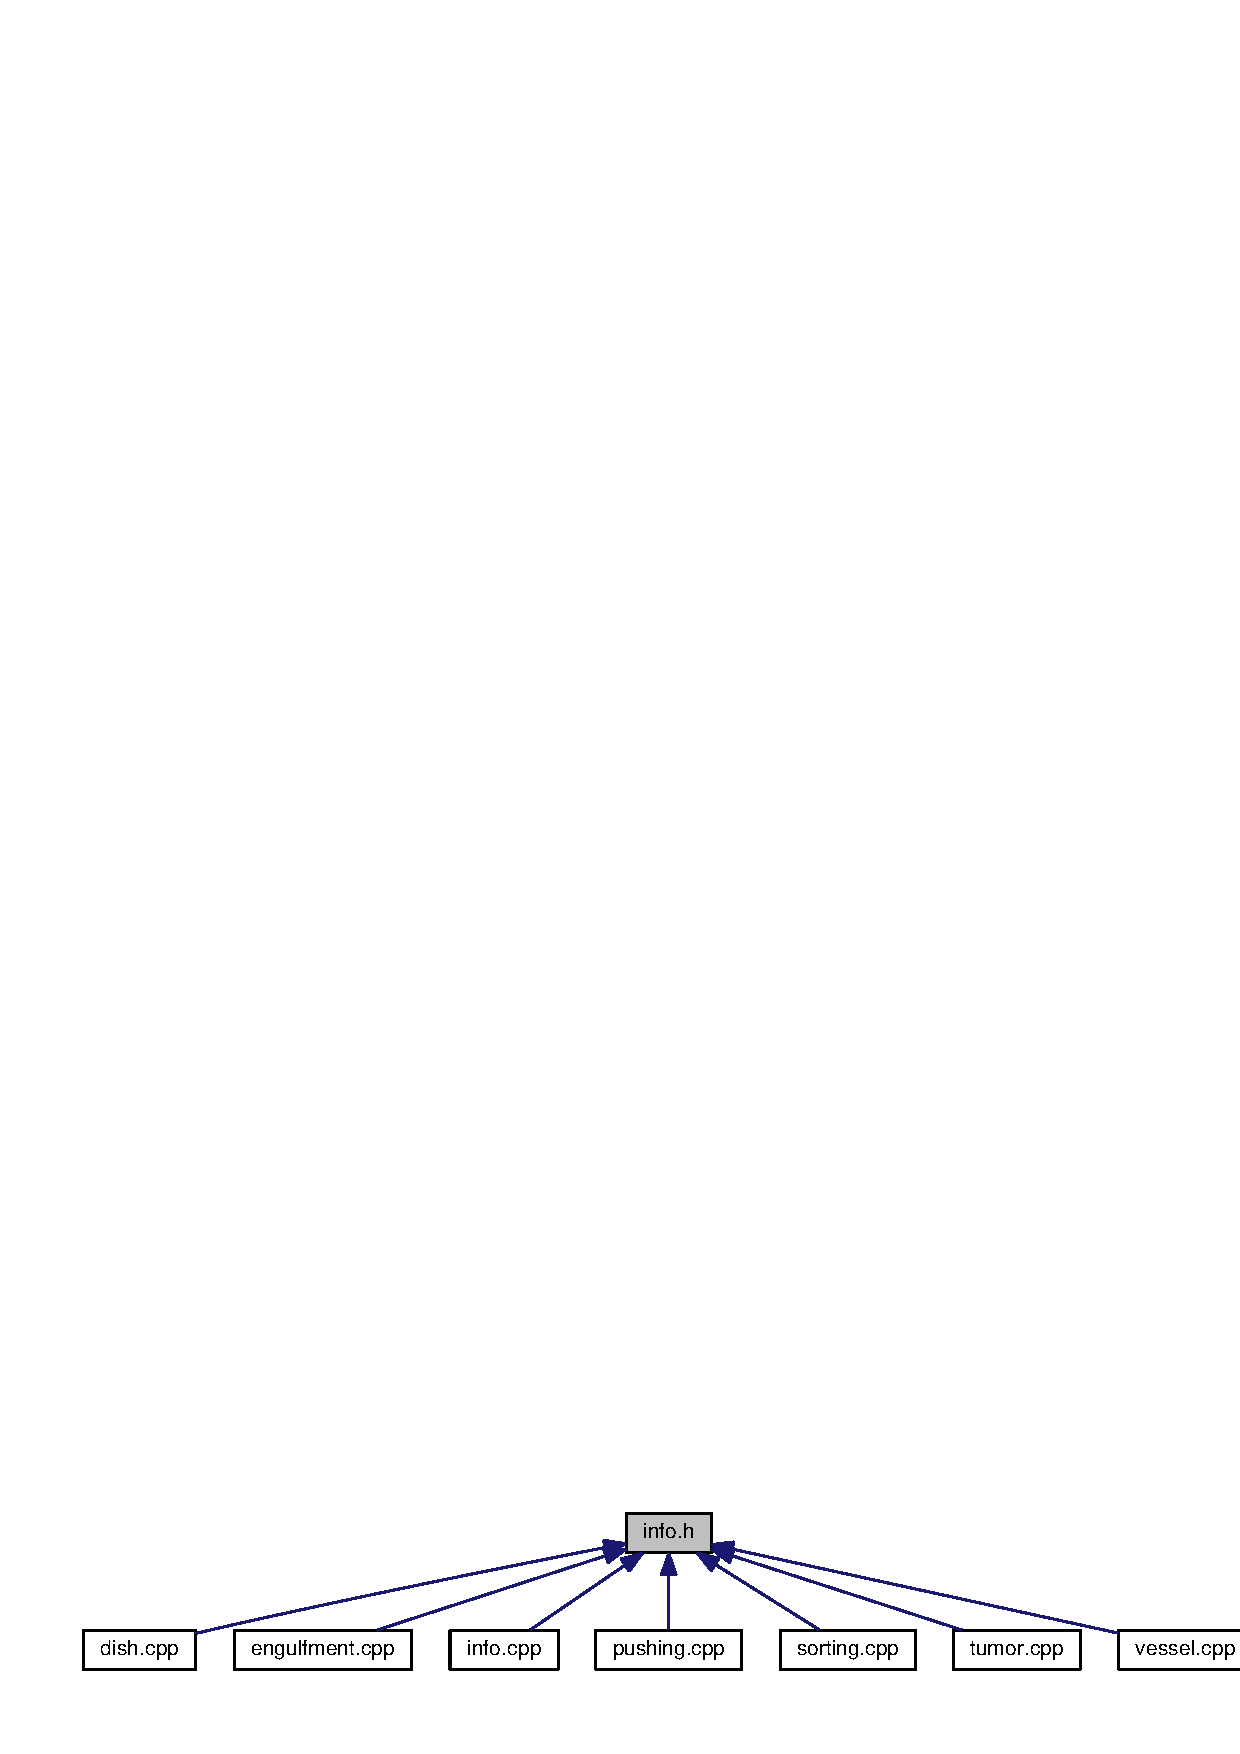
\includegraphics[width=350pt]{info_8h__dep__incl}
\end{center}
\end{figure}
\subsection*{Classes}
\begin{DoxyCompactItemize}
\item 
class {\bf Info}
\begin{DoxyCompactList}\small\item\em Enables interactive querying of the simulation. \end{DoxyCompactList}\end{DoxyCompactItemize}

\section{mainpage.\-h File Reference}
\label{mainpage_8h}\index{mainpage.\-h@{mainpage.\-h}}
This graph shows which files directly or indirectly include this file\-:
\nopagebreak
\begin{figure}[H]
\begin{center}
\leavevmode
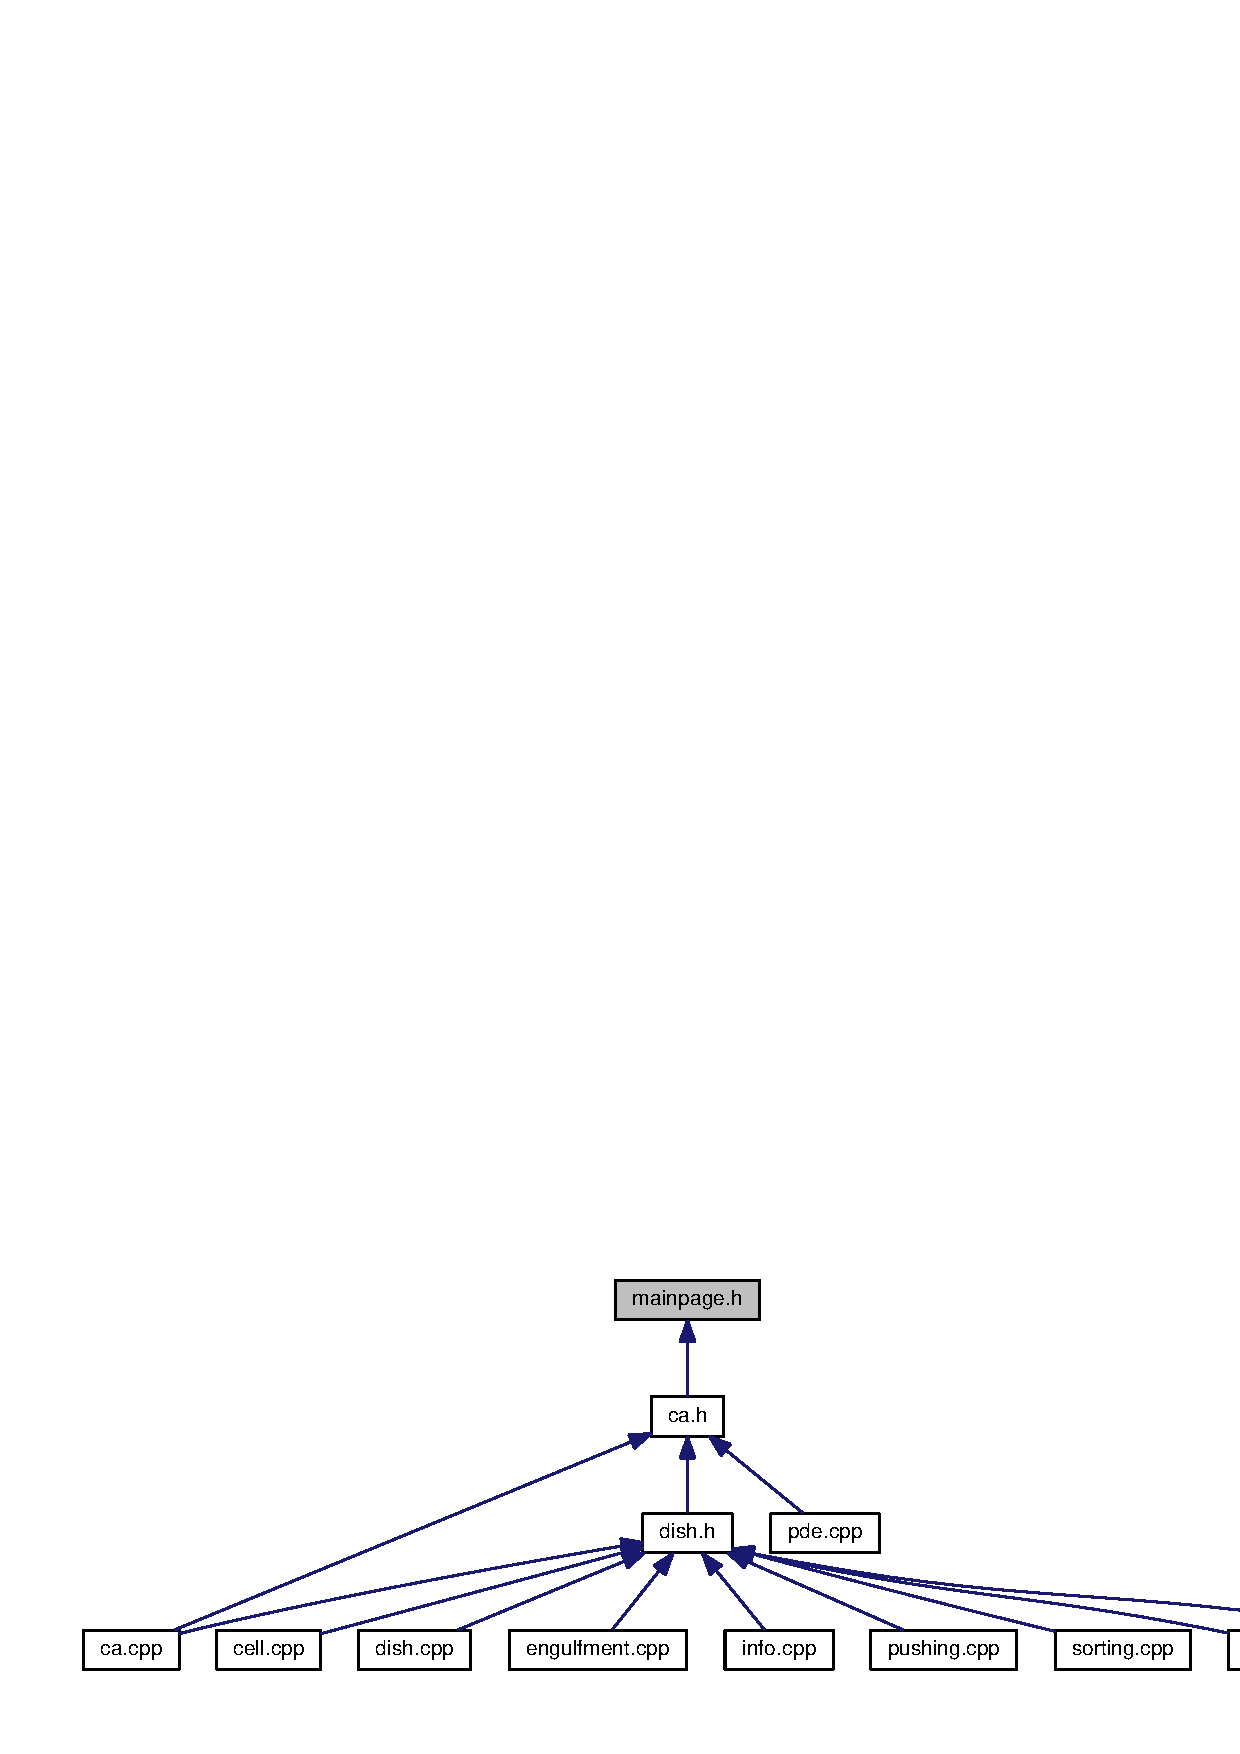
\includegraphics[width=350pt]{mainpage_8h__dep__incl}
\end{center}
\end{figure}

\section{misc.\-cpp File Reference}
\label{misc_8cpp}\index{misc.\-cpp@{misc.\-cpp}}
{\ttfamily \#include $<$stdio.\-h$>$}\\*
{\ttfamily \#include $<$locale.\-h$>$}\\*
{\ttfamily \#include $<$stdlib.\-h$>$}\\*
{\ttfamily \#include $<$cstring$>$}\\*
{\ttfamily \#include \char`\"{}sticky.\-h\char`\"{}}\\*
Include dependency graph for misc.\-cpp\-:
\nopagebreak
\begin{figure}[H]
\begin{center}
\leavevmode
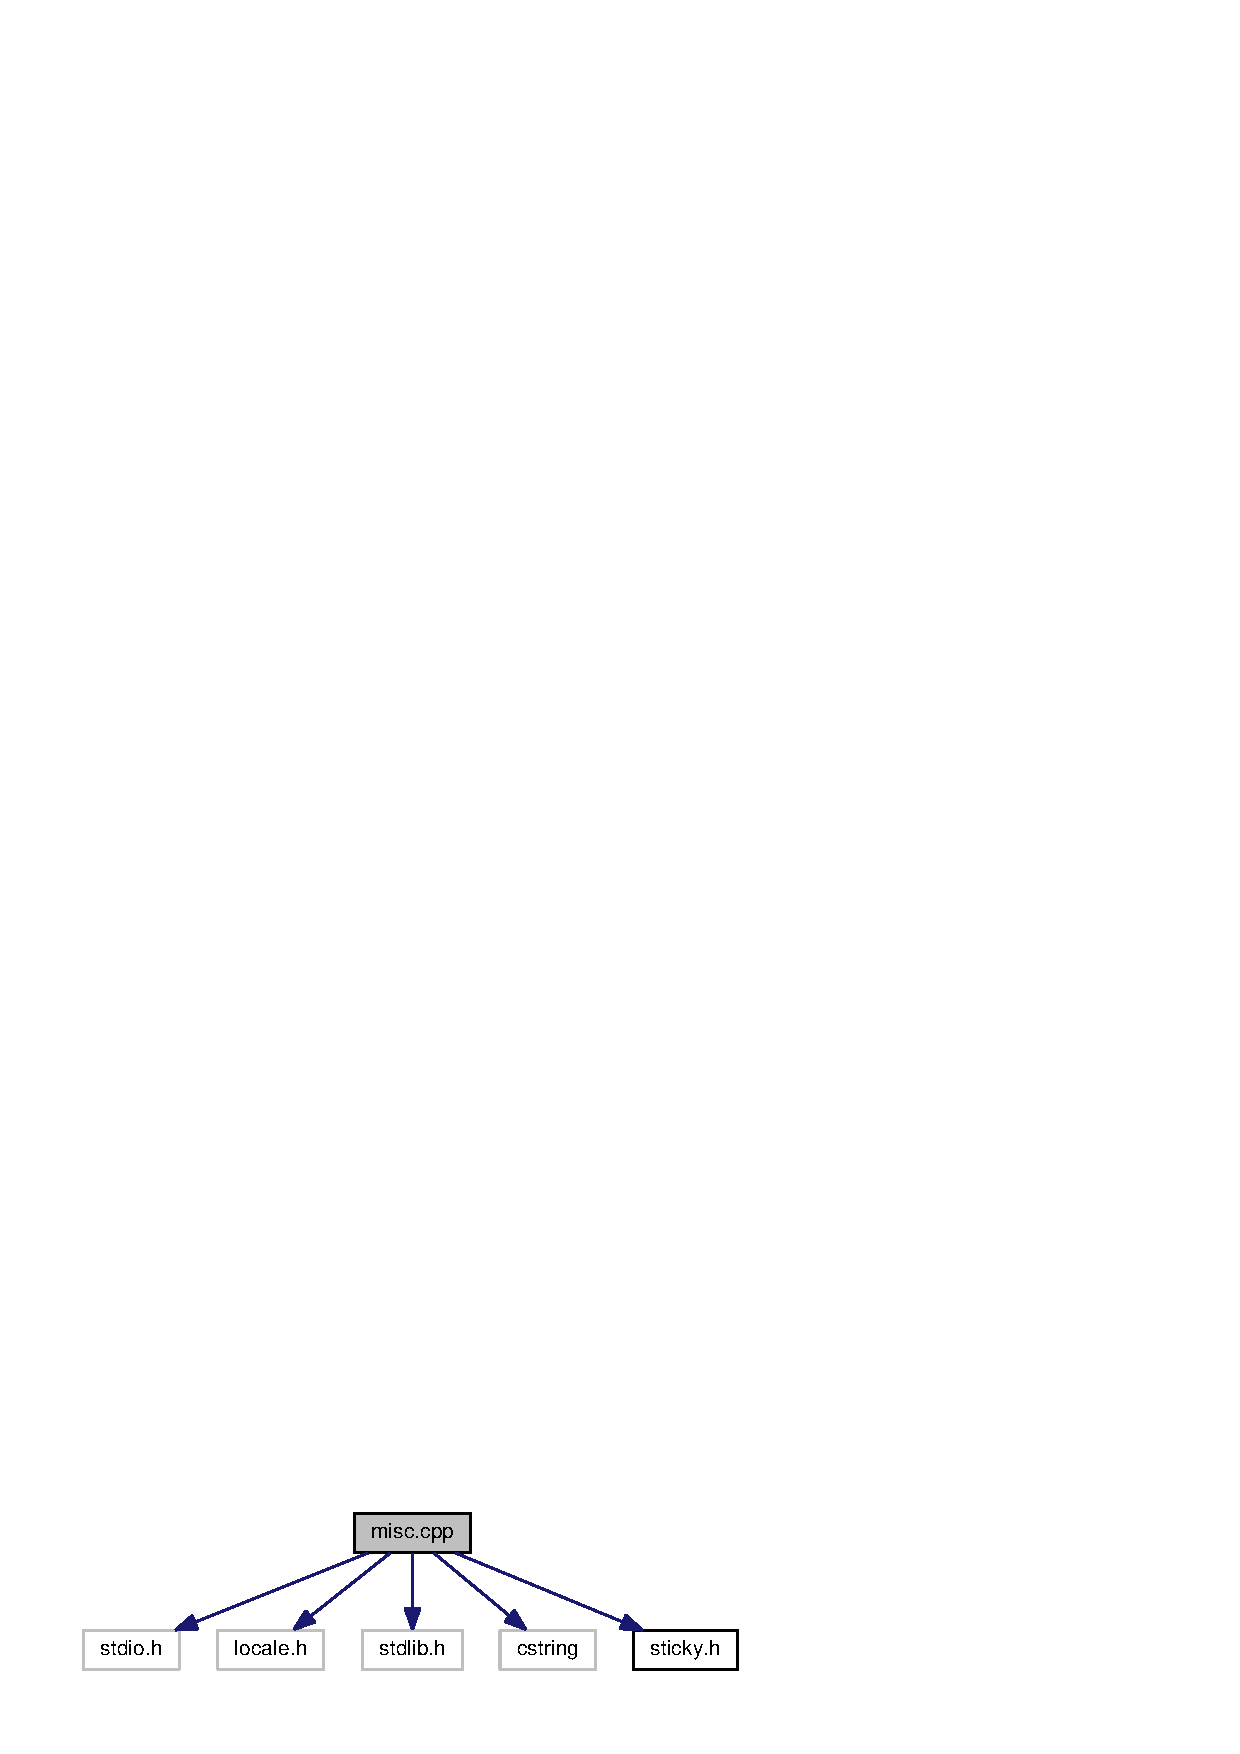
\includegraphics[width=350pt]{misc_8cpp__incl}
\end{center}
\end{figure}
\subsection*{Functions}
\begin{DoxyCompactItemize}
\item 
int {\bf Read\-Number} (F\-I\-L\-E $\ast$file, int $\ast$number)
\item 
int {\bf Read\-Double} (F\-I\-L\-E $\ast$file, double $\ast$number)
\item 
int {\bf File\-Exists} (F\-I\-L\-E $\ast$$\ast$fp, const char $\ast$fname, const char $\ast$ftype)
\item 
int {\bf Yes\-No\-P} (const char $\ast$message)
\item 
char $\ast$ {\bf Get\-File\-Name} (const char $\ast$message, const char $\ast$ftype)
\end{DoxyCompactItemize}


\subsection{Function Documentation}
\index{misc.\-cpp@{misc.\-cpp}!File\-Exists@{File\-Exists}}
\index{File\-Exists@{File\-Exists}!misc.cpp@{misc.\-cpp}}
\subsubsection[{File\-Exists}]{\setlength{\rightskip}{0pt plus 5cm}int File\-Exists (
\begin{DoxyParamCaption}
\item[{F\-I\-L\-E $\ast$$\ast$}]{fp, }
\item[{const char $\ast$}]{fname, }
\item[{const char $\ast$}]{ftype}
\end{DoxyParamCaption}
)}\label{misc_8cpp_ae59164878311b840e5846c64ae238126}


References F\-A\-L\-S\-E, and T\-R\-U\-E.



Referenced by Get\-File\-Name().

\index{misc.\-cpp@{misc.\-cpp}!Get\-File\-Name@{Get\-File\-Name}}
\index{Get\-File\-Name@{Get\-File\-Name}!misc.cpp@{misc.\-cpp}}
\subsubsection[{Get\-File\-Name}]{\setlength{\rightskip}{0pt plus 5cm}char$\ast$ Get\-File\-Name (
\begin{DoxyParamCaption}
\item[{const char $\ast$}]{message, }
\item[{const char $\ast$}]{ftype}
\end{DoxyParamCaption}
)}\label{misc_8cpp_afbd8290f9c5b53b8ec8b86a06bdd6ac0}


References F\-A\-L\-S\-E, File\-Exists(), T\-R\-U\-E, and Yes\-No\-P().

\index{misc.\-cpp@{misc.\-cpp}!Read\-Double@{Read\-Double}}
\index{Read\-Double@{Read\-Double}!misc.cpp@{misc.\-cpp}}
\subsubsection[{Read\-Double}]{\setlength{\rightskip}{0pt plus 5cm}int Read\-Double (
\begin{DoxyParamCaption}
\item[{F\-I\-L\-E $\ast$}]{file, }
\item[{double $\ast$}]{number}
\end{DoxyParamCaption}
)}\label{misc_8cpp_a1065caf5bb7bf5a871c0bb6cce4e5d69}


References O\-K, and R\-E\-M\-A\-R\-K.



Referenced by Info\-::\-Menu().

\index{misc.\-cpp@{misc.\-cpp}!Read\-Number@{Read\-Number}}
\index{Read\-Number@{Read\-Number}!misc.cpp@{misc.\-cpp}}
\subsubsection[{Read\-Number}]{\setlength{\rightskip}{0pt plus 5cm}int Read\-Number (
\begin{DoxyParamCaption}
\item[{F\-I\-L\-E $\ast$}]{file, }
\item[{int $\ast$}]{number}
\end{DoxyParamCaption}
)}\label{misc_8cpp_ab1000566635b3292ea889a41b92f12b2}
P\-U\-B\-L\-I\-C 

References O\-K, and R\-E\-M\-A\-R\-K.

\index{misc.\-cpp@{misc.\-cpp}!Yes\-No\-P@{Yes\-No\-P}}
\index{Yes\-No\-P@{Yes\-No\-P}!misc.cpp@{misc.\-cpp}}
\subsubsection[{Yes\-No\-P}]{\setlength{\rightskip}{0pt plus 5cm}int Yes\-No\-P (
\begin{DoxyParamCaption}
\item[{const char $\ast$}]{message}
\end{DoxyParamCaption}
)}\label{misc_8cpp_aa67ef0a1d41408ed07b342be6de4c37c}


Referenced by Get\-File\-Name(), and Info\-::\-Menu().


\section{misc.\-h File Reference}
\label{misc_8h}\index{misc.\-h@{misc.\-h}}
This graph shows which files directly or indirectly include this file\-:
\nopagebreak
\begin{figure}[H]
\begin{center}
\leavevmode
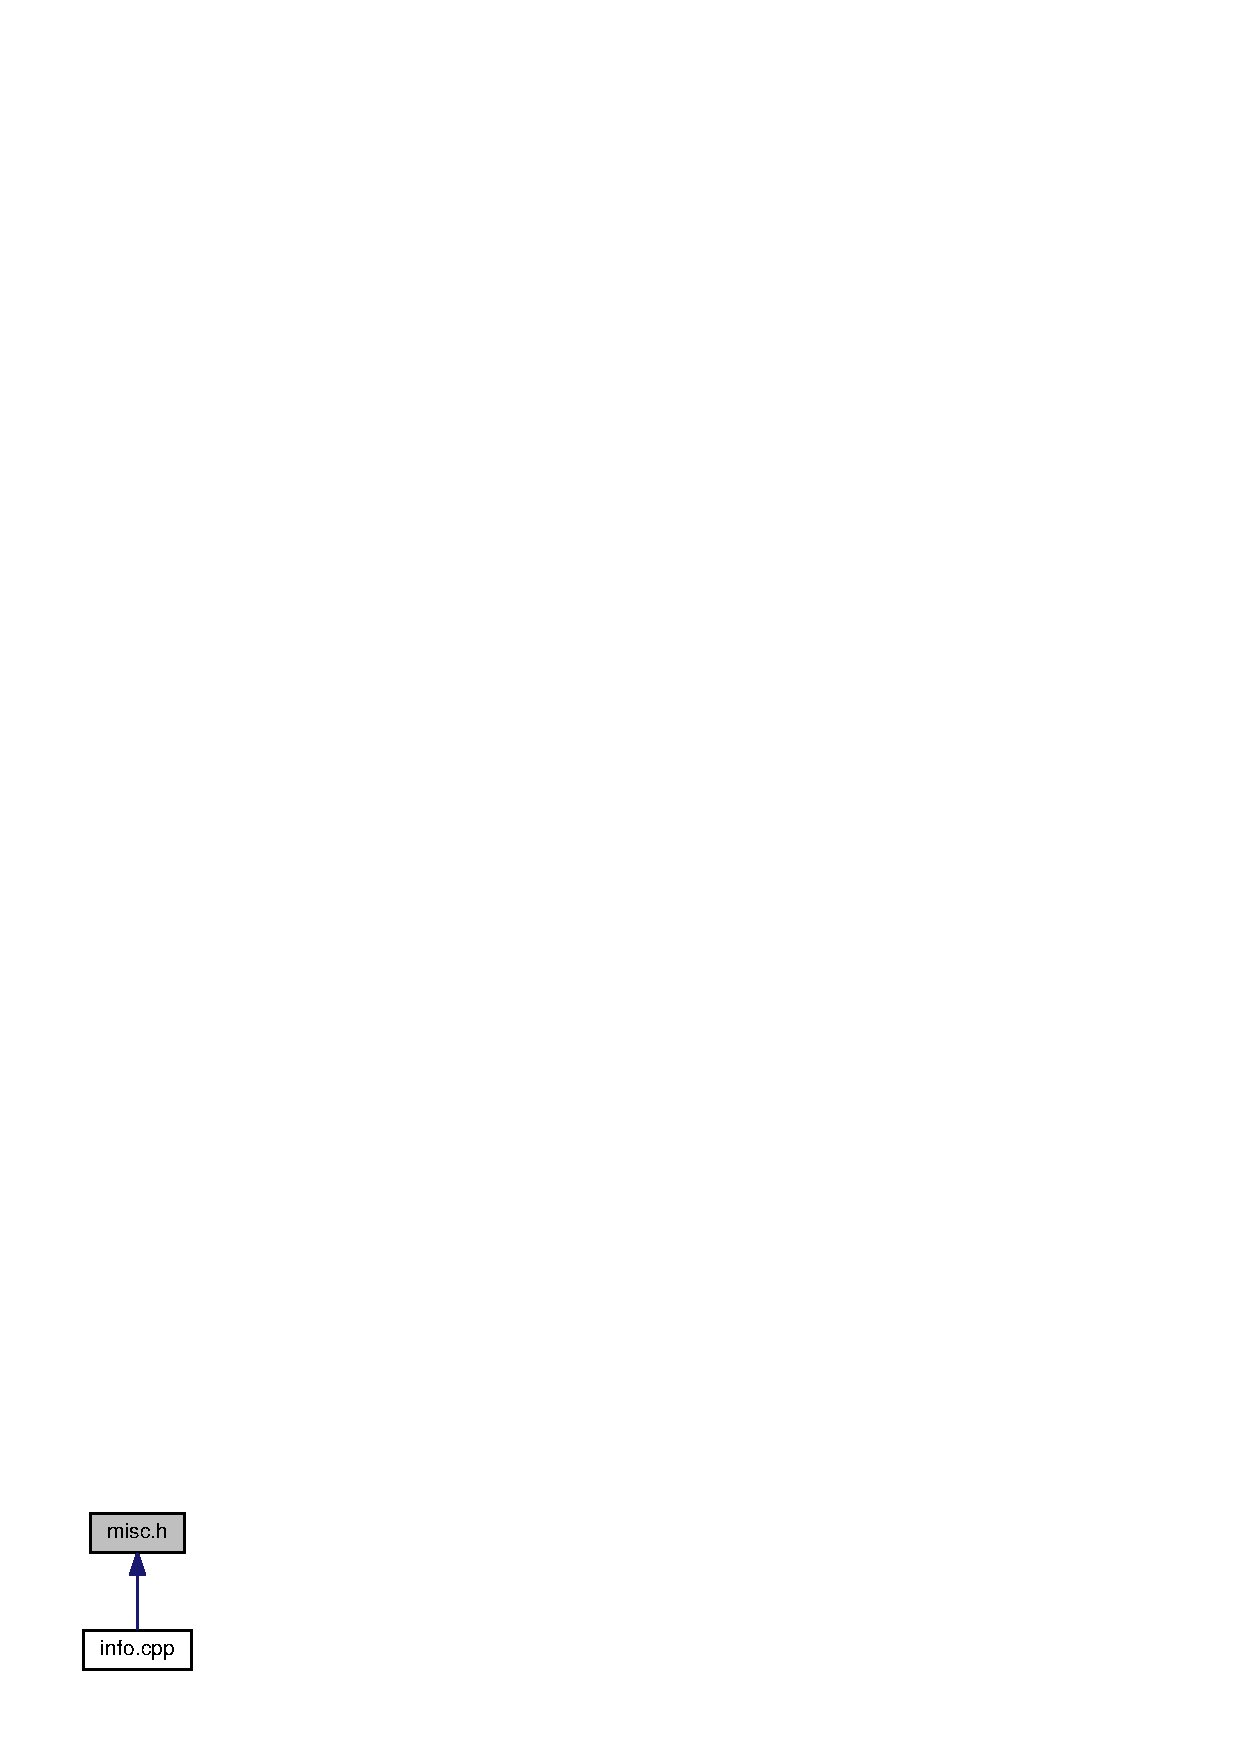
\includegraphics[width=96pt]{misc_8h__dep__incl}
\end{center}
\end{figure}
\subsection*{Macros}
\begin{DoxyCompactItemize}
\item 
\#define {\bf F\-A\-L\-S\-E}~0
\item 
\#define {\bf T\-R\-U\-E}~1
\item 
\#define {\bf O\-K}~1
\item 
\#define {\bf R\-E\-M\-A\-R\-K}~56
\end{DoxyCompactItemize}
\subsection*{Functions}
\begin{DoxyCompactItemize}
\item 
int {\bf Read\-Number} (F\-I\-L\-E $\ast$file, int $\ast$number)
\item 
int {\bf Yes\-No\-P} (const char $\ast$message)
\item 
char $\ast$ {\bf Get\-File\-Name} (const char $\ast$message, const char $\ast$ftype)
\item 
int {\bf File\-Exists} (F\-I\-L\-E $\ast$$\ast$fp, const char $\ast$fname, const char $\ast$ftype)
\item 
int {\bf Read\-Double} (F\-I\-L\-E $\ast$file, double $\ast$number)
\end{DoxyCompactItemize}


\subsection{Macro Definition Documentation}
\index{misc.\-h@{misc.\-h}!F\-A\-L\-S\-E@{F\-A\-L\-S\-E}}
\index{F\-A\-L\-S\-E@{F\-A\-L\-S\-E}!misc.h@{misc.\-h}}
\subsubsection[{F\-A\-L\-S\-E}]{\setlength{\rightskip}{0pt plus 5cm}\#define F\-A\-L\-S\-E~0}\label{misc_8h_aa93f0eb578d23995850d61f7d61c55c1}


Referenced by File\-Exists(), File\-Exists\-P(), Get\-File\-Name(), Open\-File\-And\-Check\-Existance(), Open\-Read\-File(), and Yes\-No\-P().

\index{misc.\-h@{misc.\-h}!O\-K@{O\-K}}
\index{O\-K@{O\-K}!misc.h@{misc.\-h}}
\subsubsection[{O\-K}]{\setlength{\rightskip}{0pt plus 5cm}\#define O\-K~1}\label{misc_8h_aba51915c87d64af47fb1cc59348961c9}


Referenced by Read\-Double(), and Read\-Number().

\index{misc.\-h@{misc.\-h}!R\-E\-M\-A\-R\-K@{R\-E\-M\-A\-R\-K}}
\index{R\-E\-M\-A\-R\-K@{R\-E\-M\-A\-R\-K}!misc.h@{misc.\-h}}
\subsubsection[{R\-E\-M\-A\-R\-K}]{\setlength{\rightskip}{0pt plus 5cm}\#define R\-E\-M\-A\-R\-K~56}\label{misc_8h_ace9fba7267bf6a9a92654ce7f25c5516}


Referenced by Read\-Double(), and Read\-Number().

\index{misc.\-h@{misc.\-h}!T\-R\-U\-E@{T\-R\-U\-E}}
\index{T\-R\-U\-E@{T\-R\-U\-E}!misc.h@{misc.\-h}}
\subsubsection[{T\-R\-U\-E}]{\setlength{\rightskip}{0pt plus 5cm}\#define T\-R\-U\-E~1}\label{misc_8h_aa8cecfc5c5c054d2875c03e77b7be15d}


Referenced by File\-Exists(), File\-Exists\-P(), Get\-File\-Name(), Open\-File\-And\-Check\-Existance(), Open\-Write\-File(), X11\-Graphics\-::\-Replace\-Beast(), and Yes\-No\-P().



\subsection{Function Documentation}
\index{misc.\-h@{misc.\-h}!File\-Exists@{File\-Exists}}
\index{File\-Exists@{File\-Exists}!misc.h@{misc.\-h}}
\subsubsection[{File\-Exists}]{\setlength{\rightskip}{0pt plus 5cm}int File\-Exists (
\begin{DoxyParamCaption}
\item[{F\-I\-L\-E $\ast$$\ast$}]{fp, }
\item[{const char $\ast$}]{fname, }
\item[{const char $\ast$}]{ftype}
\end{DoxyParamCaption}
)}\label{misc_8h_ae59164878311b840e5846c64ae238126}


References F\-A\-L\-S\-E, and T\-R\-U\-E.



Referenced by Get\-File\-Name().

\index{misc.\-h@{misc.\-h}!Get\-File\-Name@{Get\-File\-Name}}
\index{Get\-File\-Name@{Get\-File\-Name}!misc.h@{misc.\-h}}
\subsubsection[{Get\-File\-Name}]{\setlength{\rightskip}{0pt plus 5cm}char$\ast$ Get\-File\-Name (
\begin{DoxyParamCaption}
\item[{const char $\ast$}]{message, }
\item[{const char $\ast$}]{ftype}
\end{DoxyParamCaption}
)}\label{misc_8h_afbd8290f9c5b53b8ec8b86a06bdd6ac0}


References F\-A\-L\-S\-E, File\-Exists(), T\-R\-U\-E, and Yes\-No\-P().

\index{misc.\-h@{misc.\-h}!Read\-Double@{Read\-Double}}
\index{Read\-Double@{Read\-Double}!misc.h@{misc.\-h}}
\subsubsection[{Read\-Double}]{\setlength{\rightskip}{0pt plus 5cm}int Read\-Double (
\begin{DoxyParamCaption}
\item[{F\-I\-L\-E $\ast$}]{file, }
\item[{double $\ast$}]{number}
\end{DoxyParamCaption}
)}\label{misc_8h_a1065caf5bb7bf5a871c0bb6cce4e5d69}


References O\-K, and R\-E\-M\-A\-R\-K.



Referenced by Info\-::\-Menu().

\index{misc.\-h@{misc.\-h}!Read\-Number@{Read\-Number}}
\index{Read\-Number@{Read\-Number}!misc.h@{misc.\-h}}
\subsubsection[{Read\-Number}]{\setlength{\rightskip}{0pt plus 5cm}int Read\-Number (
\begin{DoxyParamCaption}
\item[{F\-I\-L\-E $\ast$}]{file, }
\item[{int $\ast$}]{number}
\end{DoxyParamCaption}
)}\label{misc_8h_ab1000566635b3292ea889a41b92f12b2}
P\-U\-B\-L\-I\-C 

References O\-K, and R\-E\-M\-A\-R\-K.

\index{misc.\-h@{misc.\-h}!Yes\-No\-P@{Yes\-No\-P}}
\index{Yes\-No\-P@{Yes\-No\-P}!misc.h@{misc.\-h}}
\subsubsection[{Yes\-No\-P}]{\setlength{\rightskip}{0pt plus 5cm}int Yes\-No\-P (
\begin{DoxyParamCaption}
\item[{const char $\ast$}]{message}
\end{DoxyParamCaption}
)}\label{misc_8h_aa67ef0a1d41408ed07b342be6de4c37c}

\section{output.\-cpp File Reference}
\label{output_8cpp}\index{output.\-cpp@{output.\-cpp}}
{\ttfamily \#include $<$stdio.\-h$>$}\\*
{\ttfamily \#include $<$string.\-h$>$}\\*
{\ttfamily \#include $<$stdlib.\-h$>$}\\*
{\ttfamily \#include $<$errno.\-h$>$}\\*
{\ttfamily \#include $<$sys/types.\-h$>$}\\*
{\ttfamily \#include $<$sys/stat.\-h$>$}\\*
{\ttfamily \#include \char`\"{}warning.\-h\char`\"{}}\\*
{\ttfamily \#include \char`\"{}parameter.\-h\char`\"{}}\\*
{\ttfamily \#include \char`\"{}output.\-h\char`\"{}}\\*
Include dependency graph for output.\-cpp\-:
\nopagebreak
\begin{figure}[H]
\begin{center}
\leavevmode
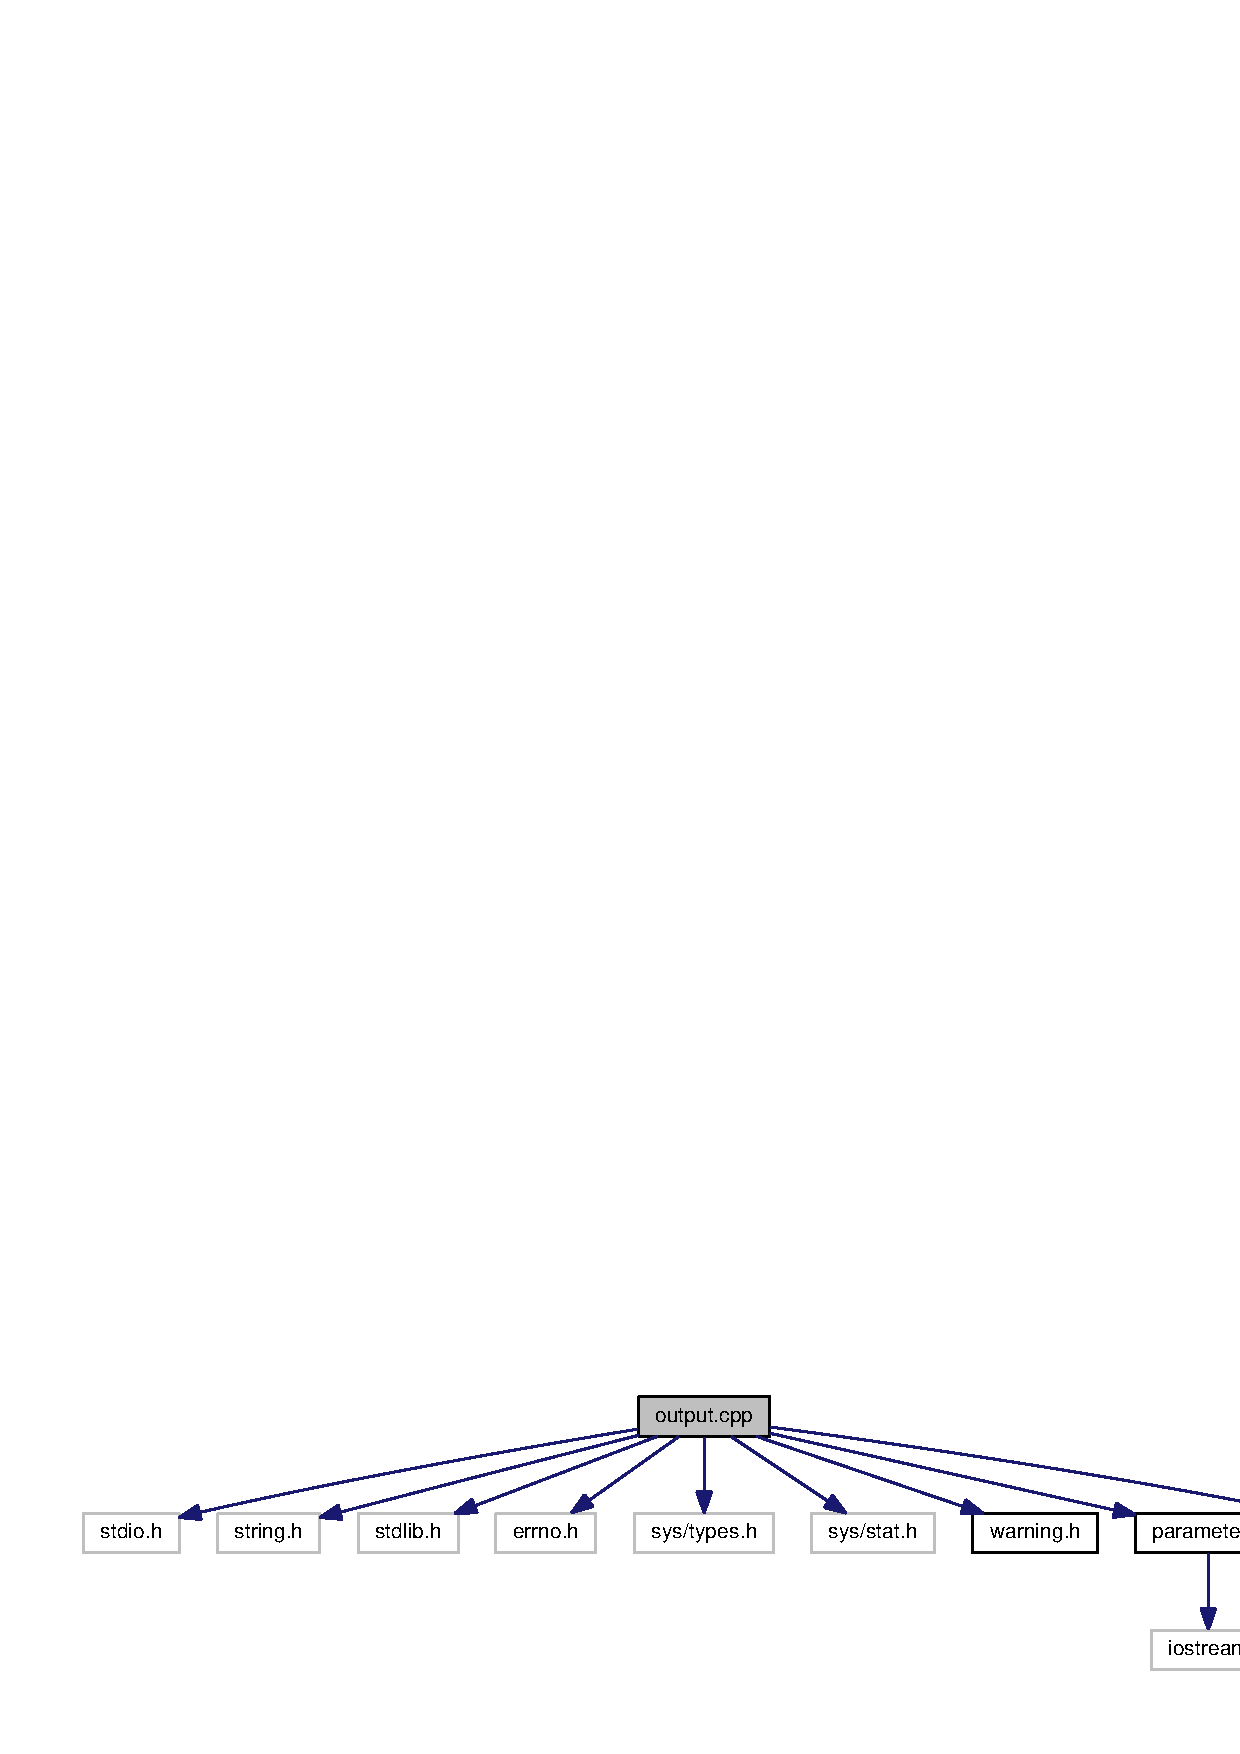
\includegraphics[width=350pt]{output_8cpp__incl}
\end{center}
\end{figure}
\subsection*{Macros}
\begin{DoxyCompactItemize}
\item 
\#define {\bf F\-N\-A\-M\-E\-S\-I\-Z\-E}~100
\item 
\#define {\bf I\-N\-I\-T\-I\-A\-L\-\_\-\-B\-U\-F\-S\-I\-Z\-E}~100
\end{DoxyCompactItemize}
\subsection*{Functions}
\begin{DoxyCompactItemize}
\item 
int {\bf Open\-File\-And\-Check\-Existance} (F\-I\-L\-E $\ast$$\ast$fp, const char $\ast$fname, char $\ast$ftype)
\item 
int {\bf File\-Exists\-P} (const char $\ast$fname)
\item 
int {\bf Yes\-No\-P} (const char $\ast$message)
\item 
F\-I\-L\-E $\ast$ {\bf Open\-Write\-File} (const char $\ast$filename)
\item 
F\-I\-L\-E $\ast$ {\bf Open\-Read\-File} (const char $\ast$filename)
\item 
char $\ast$ {\bf Read\-Line} (F\-I\-L\-E $\ast$fp)
\item 
void {\bf Check\-File} (F\-I\-L\-E $\ast$fp)
\item 
char $\ast$ {\bf Chext} (char $\ast$filename)
\end{DoxyCompactItemize}


\subsection{Macro Definition Documentation}
\index{output.\-cpp@{output.\-cpp}!F\-N\-A\-M\-E\-S\-I\-Z\-E@{F\-N\-A\-M\-E\-S\-I\-Z\-E}}
\index{F\-N\-A\-M\-E\-S\-I\-Z\-E@{F\-N\-A\-M\-E\-S\-I\-Z\-E}!output.cpp@{output.\-cpp}}
\subsubsection[{F\-N\-A\-M\-E\-S\-I\-Z\-E}]{\setlength{\rightskip}{0pt plus 5cm}\#define F\-N\-A\-M\-E\-S\-I\-Z\-E~100}\label{output_8cpp_ae83ce735482c1d710ee7664331f71875}


Referenced by Open\-Write\-File().

\index{output.\-cpp@{output.\-cpp}!I\-N\-I\-T\-I\-A\-L\-\_\-\-B\-U\-F\-S\-I\-Z\-E@{I\-N\-I\-T\-I\-A\-L\-\_\-\-B\-U\-F\-S\-I\-Z\-E}}
\index{I\-N\-I\-T\-I\-A\-L\-\_\-\-B\-U\-F\-S\-I\-Z\-E@{I\-N\-I\-T\-I\-A\-L\-\_\-\-B\-U\-F\-S\-I\-Z\-E}!output.cpp@{output.\-cpp}}
\subsubsection[{I\-N\-I\-T\-I\-A\-L\-\_\-\-B\-U\-F\-S\-I\-Z\-E}]{\setlength{\rightskip}{0pt plus 5cm}\#define I\-N\-I\-T\-I\-A\-L\-\_\-\-B\-U\-F\-S\-I\-Z\-E~100}\label{output_8cpp_afa6724360f3351cdc337471d90c7d7b1}


Referenced by Read\-Line().



\subsection{Function Documentation}
\index{output.\-cpp@{output.\-cpp}!Check\-File@{Check\-File}}
\index{Check\-File@{Check\-File}!output.cpp@{output.\-cpp}}
\subsubsection[{Check\-File}]{\setlength{\rightskip}{0pt plus 5cm}void Check\-File (
\begin{DoxyParamCaption}
\item[{F\-I\-L\-E $\ast$}]{fp}
\end{DoxyParamCaption}
)}\label{output_8cpp_a591057779cf6eb75e2b32e4bd5fd7e39}


References errno, and error().



Referenced by Read\-Line().

\index{output.\-cpp@{output.\-cpp}!Chext@{Chext}}
\index{Chext@{Chext}!output.cpp@{output.\-cpp}}
\subsubsection[{Chext}]{\setlength{\rightskip}{0pt plus 5cm}char$\ast$ Chext (
\begin{DoxyParamCaption}
\item[{char $\ast$}]{filename}
\end{DoxyParamCaption}
)}\label{output_8cpp_aed9addb9669ade1f4f253421d2e584e8}
\index{output.\-cpp@{output.\-cpp}!File\-Exists\-P@{File\-Exists\-P}}
\index{File\-Exists\-P@{File\-Exists\-P}!output.cpp@{output.\-cpp}}
\subsubsection[{File\-Exists\-P}]{\setlength{\rightskip}{0pt plus 5cm}int File\-Exists\-P (
\begin{DoxyParamCaption}
\item[{const char $\ast$}]{fname}
\end{DoxyParamCaption}
)}\label{output_8cpp_a077e75dac8ec098c48f371324d242125}


References F\-A\-L\-S\-E, and T\-R\-U\-E.



Referenced by Open\-Write\-File().

\index{output.\-cpp@{output.\-cpp}!Open\-File\-And\-Check\-Existance@{Open\-File\-And\-Check\-Existance}}
\index{Open\-File\-And\-Check\-Existance@{Open\-File\-And\-Check\-Existance}!output.cpp@{output.\-cpp}}
\subsubsection[{Open\-File\-And\-Check\-Existance}]{\setlength{\rightskip}{0pt plus 5cm}int Open\-File\-And\-Check\-Existance (
\begin{DoxyParamCaption}
\item[{F\-I\-L\-E $\ast$$\ast$}]{fp, }
\item[{const char $\ast$}]{fname, }
\item[{char $\ast$}]{ftype}
\end{DoxyParamCaption}
)}\label{output_8cpp_ae2d304b679f192150c7d56a96f704dea}


References F\-A\-L\-S\-E, and T\-R\-U\-E.



Referenced by Open\-Read\-File().

\index{output.\-cpp@{output.\-cpp}!Open\-Read\-File@{Open\-Read\-File}}
\index{Open\-Read\-File@{Open\-Read\-File}!output.cpp@{output.\-cpp}}
\subsubsection[{Open\-Read\-File}]{\setlength{\rightskip}{0pt plus 5cm}F\-I\-L\-E$\ast$ Open\-Read\-File (
\begin{DoxyParamCaption}
\item[{const char $\ast$}]{filename}
\end{DoxyParamCaption}
)}\label{output_8cpp_ae65c4e75d7e0eec28ee29907349430d9}


References F\-A\-L\-S\-E, and Open\-File\-And\-Check\-Existance().



Referenced by Parameter\-::\-Read().

\index{output.\-cpp@{output.\-cpp}!Open\-Write\-File@{Open\-Write\-File}}
\index{Open\-Write\-File@{Open\-Write\-File}!output.cpp@{output.\-cpp}}
\subsubsection[{Open\-Write\-File}]{\setlength{\rightskip}{0pt plus 5cm}F\-I\-L\-E$\ast$ Open\-Write\-File (
\begin{DoxyParamCaption}
\item[{const char $\ast$}]{filename}
\end{DoxyParamCaption}
)}\label{output_8cpp_ae665379ae0aec10a4eba6e6e9679b368}


References File\-Exists\-P(), F\-N\-A\-M\-E\-S\-I\-Z\-E, and T\-R\-U\-E.

\index{output.\-cpp@{output.\-cpp}!Read\-Line@{Read\-Line}}
\index{Read\-Line@{Read\-Line}!output.cpp@{output.\-cpp}}
\subsubsection[{Read\-Line}]{\setlength{\rightskip}{0pt plus 5cm}char$\ast$ Read\-Line (
\begin{DoxyParamCaption}
\item[{F\-I\-L\-E $\ast$}]{fp}
\end{DoxyParamCaption}
)}\label{output_8cpp_aa1a5a5360af42ce9059dc52134fdac41}


References Check\-File(), errno, error(), I\-N\-I\-T\-I\-A\-L\-\_\-\-B\-U\-F\-S\-I\-Z\-E, and M\-E\-M\-O\-R\-Y\-C\-H\-E\-C\-K.



Referenced by Search\-Token(), and Skip\-Line().

\index{output.\-cpp@{output.\-cpp}!Yes\-No\-P@{Yes\-No\-P}}
\index{Yes\-No\-P@{Yes\-No\-P}!output.cpp@{output.\-cpp}}
\subsubsection[{Yes\-No\-P}]{\setlength{\rightskip}{0pt plus 5cm}int Yes\-No\-P (
\begin{DoxyParamCaption}
\item[{const char $\ast$}]{message}
\end{DoxyParamCaption}
)}\label{output_8cpp_aa67ef0a1d41408ed07b342be6de4c37c}


References F\-A\-L\-S\-E, and T\-R\-U\-E.


\section{output.\-h File Reference}
\label{output_8h}\index{output.\-h@{output.\-h}}
This graph shows which files directly or indirectly include this file\-:
\nopagebreak
\begin{figure}[H]
\begin{center}
\leavevmode
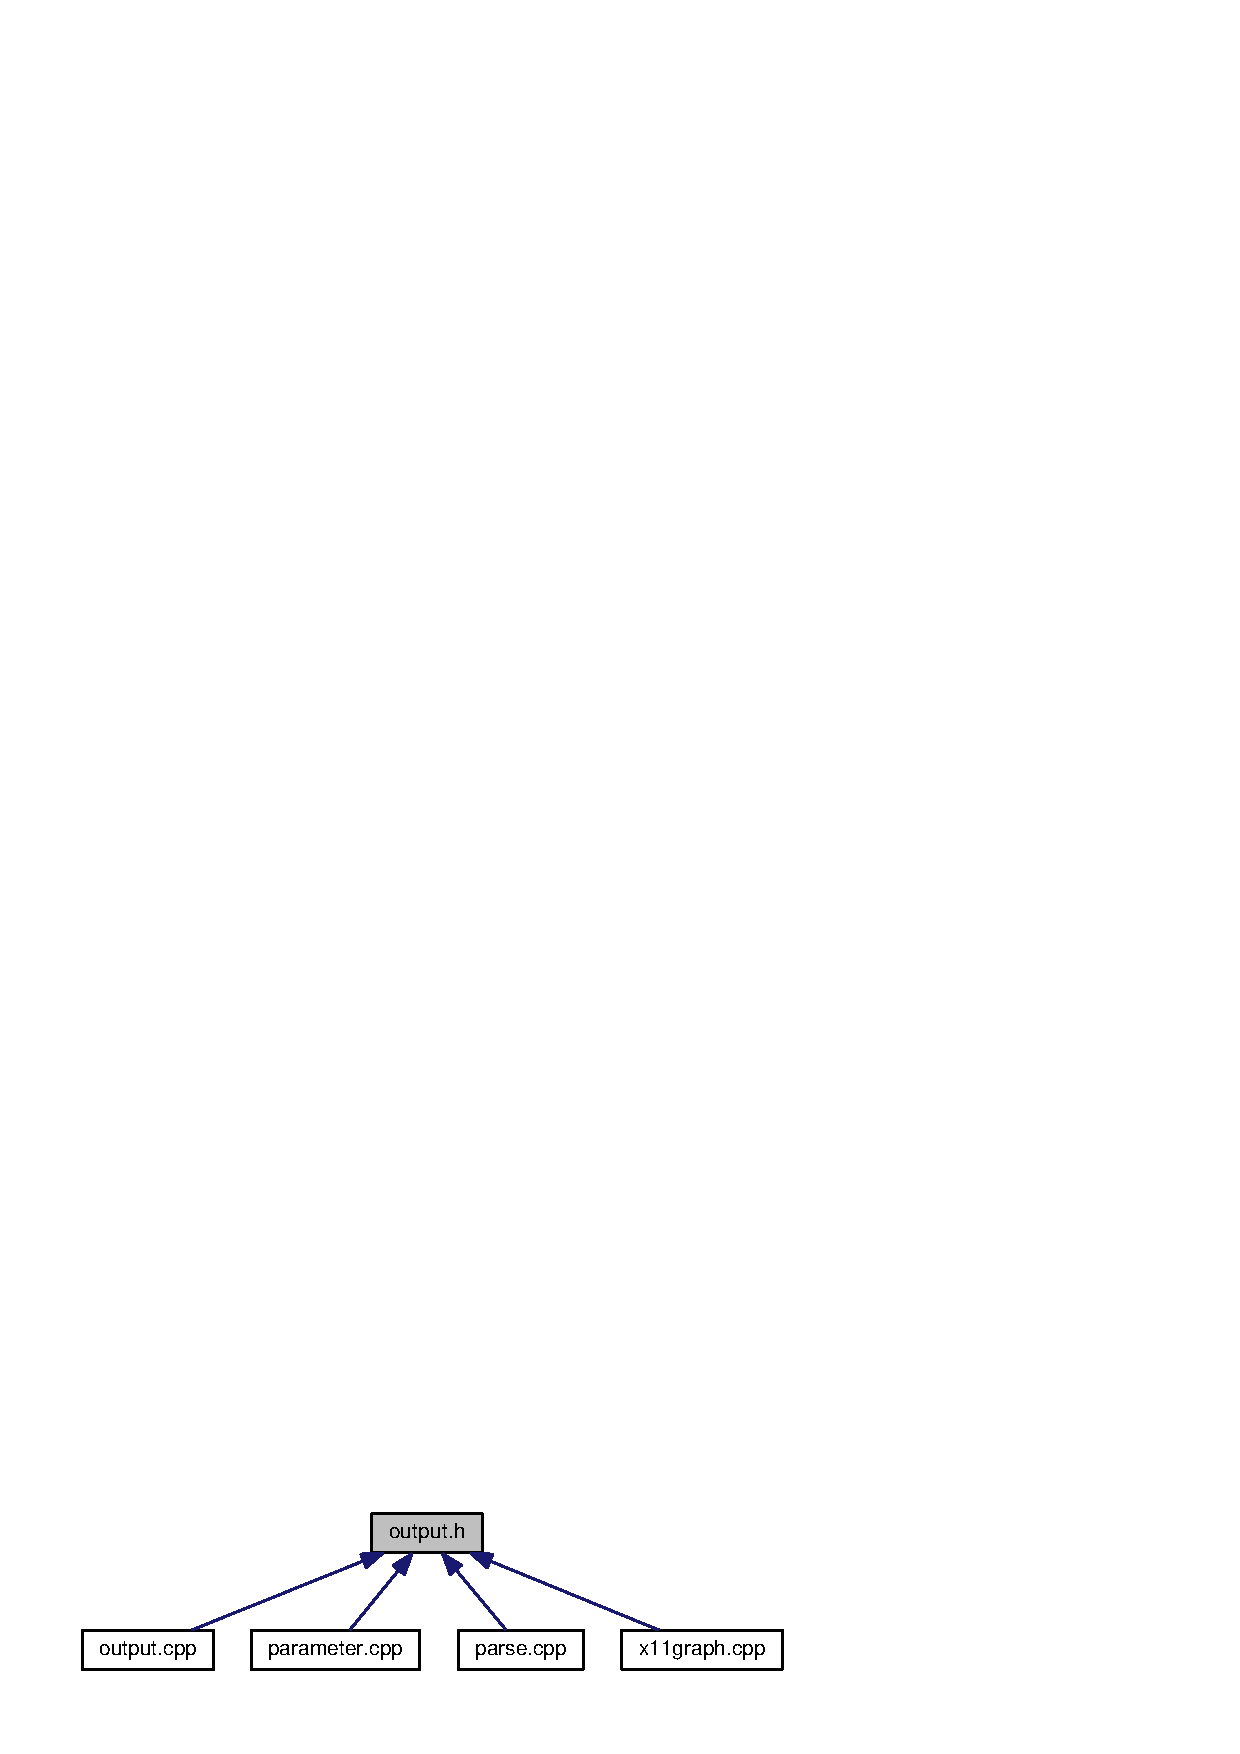
\includegraphics[width=350pt]{output_8h__dep__incl}
\end{center}
\end{figure}
\subsection*{Macros}
\begin{DoxyCompactItemize}
\item 
\#define {\bf M\-E\-S\-S\-\_\-\-B\-U\-F\-\_\-\-S\-I\-Z\-E}~160
\item 
\#define {\bf F\-A\-L\-S\-E}~0
\item 
\#define {\bf T\-R\-U\-E}~1
\end{DoxyCompactItemize}
\subsection*{Functions}
\begin{DoxyCompactItemize}
\item 
int {\bf Open\-File\-And\-Check\-Existance} (F\-I\-L\-E $\ast$$\ast$fp, const char $\ast$fname, char $\ast$ftype)
\item 
int {\bf Yes\-No\-P} (const char $\ast$message)
\item 
F\-I\-L\-E $\ast$ {\bf Open\-Write\-File} (const char $\ast$filename)
\item 
F\-I\-L\-E $\ast$ {\bf Open\-G\-Zipped\-Write\-File} (const char $\ast$filename)
\item 
F\-I\-L\-E $\ast$ {\bf Open\-Read\-File} (const char $\ast$filename)
\item 
char $\ast$ {\bf Read\-Line} (F\-I\-L\-E $\ast$fp)
\item 
void {\bf Check\-File} (F\-I\-L\-E $\ast$fp)
\item 
int {\bf File\-Exists\-P} (const char $\ast$fname)
\item 
char $\ast$ {\bf Chext} (char $\ast$filename)
\item 
void {\bf Make\-Dir} (const char $\ast$dirname)
\item 
bool {\bf Can\-We\-Write\-P} (char $\ast$filename)
\end{DoxyCompactItemize}


\subsection{Macro Definition Documentation}
\index{output.\-h@{output.\-h}!F\-A\-L\-S\-E@{F\-A\-L\-S\-E}}
\index{F\-A\-L\-S\-E@{F\-A\-L\-S\-E}!output.h@{output.\-h}}
\subsubsection[{F\-A\-L\-S\-E}]{\setlength{\rightskip}{0pt plus 5cm}\#define F\-A\-L\-S\-E~0}\label{output_8h_aa93f0eb578d23995850d61f7d61c55c1}
\index{output.\-h@{output.\-h}!M\-E\-S\-S\-\_\-\-B\-U\-F\-\_\-\-S\-I\-Z\-E@{M\-E\-S\-S\-\_\-\-B\-U\-F\-\_\-\-S\-I\-Z\-E}}
\index{M\-E\-S\-S\-\_\-\-B\-U\-F\-\_\-\-S\-I\-Z\-E@{M\-E\-S\-S\-\_\-\-B\-U\-F\-\_\-\-S\-I\-Z\-E}!output.h@{output.\-h}}
\subsubsection[{M\-E\-S\-S\-\_\-\-B\-U\-F\-\_\-\-S\-I\-Z\-E}]{\setlength{\rightskip}{0pt plus 5cm}\#define M\-E\-S\-S\-\_\-\-B\-U\-F\-\_\-\-S\-I\-Z\-E~160}\label{output_8h_aba6accff3016874eb0bb95d2b197801e}
\index{output.\-h@{output.\-h}!T\-R\-U\-E@{T\-R\-U\-E}}
\index{T\-R\-U\-E@{T\-R\-U\-E}!output.h@{output.\-h}}
\subsubsection[{T\-R\-U\-E}]{\setlength{\rightskip}{0pt plus 5cm}\#define T\-R\-U\-E~1}\label{output_8h_aa8cecfc5c5c054d2875c03e77b7be15d}


\subsection{Function Documentation}
\index{output.\-h@{output.\-h}!Can\-We\-Write\-P@{Can\-We\-Write\-P}}
\index{Can\-We\-Write\-P@{Can\-We\-Write\-P}!output.h@{output.\-h}}
\subsubsection[{Can\-We\-Write\-P}]{\setlength{\rightskip}{0pt plus 5cm}bool Can\-We\-Write\-P (
\begin{DoxyParamCaption}
\item[{char $\ast$}]{filename}
\end{DoxyParamCaption}
)}\label{output_8h_af74935c6d7742547b2a1381a8a26d683}
\index{output.\-h@{output.\-h}!Check\-File@{Check\-File}}
\index{Check\-File@{Check\-File}!output.h@{output.\-h}}
\subsubsection[{Check\-File}]{\setlength{\rightskip}{0pt plus 5cm}void Check\-File (
\begin{DoxyParamCaption}
\item[{F\-I\-L\-E $\ast$}]{fp}
\end{DoxyParamCaption}
)}\label{output_8h_a591057779cf6eb75e2b32e4bd5fd7e39}


References errno, and error().



Referenced by Read\-Line().

\index{output.\-h@{output.\-h}!Chext@{Chext}}
\index{Chext@{Chext}!output.h@{output.\-h}}
\subsubsection[{Chext}]{\setlength{\rightskip}{0pt plus 5cm}char$\ast$ Chext (
\begin{DoxyParamCaption}
\item[{char $\ast$}]{filename}
\end{DoxyParamCaption}
)}\label{output_8h_aed9addb9669ade1f4f253421d2e584e8}
\index{output.\-h@{output.\-h}!File\-Exists\-P@{File\-Exists\-P}}
\index{File\-Exists\-P@{File\-Exists\-P}!output.h@{output.\-h}}
\subsubsection[{File\-Exists\-P}]{\setlength{\rightskip}{0pt plus 5cm}int File\-Exists\-P (
\begin{DoxyParamCaption}
\item[{const char $\ast$}]{fname}
\end{DoxyParamCaption}
)}\label{output_8h_a077e75dac8ec098c48f371324d242125}


References F\-A\-L\-S\-E, and T\-R\-U\-E.



Referenced by Open\-Write\-File().

\index{output.\-h@{output.\-h}!Make\-Dir@{Make\-Dir}}
\index{Make\-Dir@{Make\-Dir}!output.h@{output.\-h}}
\subsubsection[{Make\-Dir}]{\setlength{\rightskip}{0pt plus 5cm}void Make\-Dir (
\begin{DoxyParamCaption}
\item[{const char $\ast$}]{dirname}
\end{DoxyParamCaption}
)}\label{output_8h_a4ec3db460f292e18639f4108c49e857d}
\index{output.\-h@{output.\-h}!Open\-File\-And\-Check\-Existance@{Open\-File\-And\-Check\-Existance}}
\index{Open\-File\-And\-Check\-Existance@{Open\-File\-And\-Check\-Existance}!output.h@{output.\-h}}
\subsubsection[{Open\-File\-And\-Check\-Existance}]{\setlength{\rightskip}{0pt plus 5cm}int Open\-File\-And\-Check\-Existance (
\begin{DoxyParamCaption}
\item[{F\-I\-L\-E $\ast$$\ast$}]{fp, }
\item[{const char $\ast$}]{fname, }
\item[{char $\ast$}]{ftype}
\end{DoxyParamCaption}
)}\label{output_8h_ae2d304b679f192150c7d56a96f704dea}


References F\-A\-L\-S\-E, and T\-R\-U\-E.



Referenced by Open\-Read\-File().

\index{output.\-h@{output.\-h}!Open\-G\-Zipped\-Write\-File@{Open\-G\-Zipped\-Write\-File}}
\index{Open\-G\-Zipped\-Write\-File@{Open\-G\-Zipped\-Write\-File}!output.h@{output.\-h}}
\subsubsection[{Open\-G\-Zipped\-Write\-File}]{\setlength{\rightskip}{0pt plus 5cm}F\-I\-L\-E$\ast$ Open\-G\-Zipped\-Write\-File (
\begin{DoxyParamCaption}
\item[{const char $\ast$}]{filename}
\end{DoxyParamCaption}
)}\label{output_8h_a75d34fa70e8aef991b63e667db9beb32}
\index{output.\-h@{output.\-h}!Open\-Read\-File@{Open\-Read\-File}}
\index{Open\-Read\-File@{Open\-Read\-File}!output.h@{output.\-h}}
\subsubsection[{Open\-Read\-File}]{\setlength{\rightskip}{0pt plus 5cm}F\-I\-L\-E$\ast$ Open\-Read\-File (
\begin{DoxyParamCaption}
\item[{const char $\ast$}]{filename}
\end{DoxyParamCaption}
)}\label{output_8h_ae65c4e75d7e0eec28ee29907349430d9}


References F\-A\-L\-S\-E, and Open\-File\-And\-Check\-Existance().



Referenced by Parameter\-::\-Read().

\index{output.\-h@{output.\-h}!Open\-Write\-File@{Open\-Write\-File}}
\index{Open\-Write\-File@{Open\-Write\-File}!output.h@{output.\-h}}
\subsubsection[{Open\-Write\-File}]{\setlength{\rightskip}{0pt plus 5cm}F\-I\-L\-E$\ast$ Open\-Write\-File (
\begin{DoxyParamCaption}
\item[{const char $\ast$}]{filename}
\end{DoxyParamCaption}
)}\label{output_8h_ae665379ae0aec10a4eba6e6e9679b368}


References File\-Exists\-P(), F\-N\-A\-M\-E\-S\-I\-Z\-E, and T\-R\-U\-E.

\index{output.\-h@{output.\-h}!Read\-Line@{Read\-Line}}
\index{Read\-Line@{Read\-Line}!output.h@{output.\-h}}
\subsubsection[{Read\-Line}]{\setlength{\rightskip}{0pt plus 5cm}char$\ast$ Read\-Line (
\begin{DoxyParamCaption}
\item[{F\-I\-L\-E $\ast$}]{fp}
\end{DoxyParamCaption}
)}\label{output_8h_aa1a5a5360af42ce9059dc52134fdac41}


References Check\-File(), errno, error(), I\-N\-I\-T\-I\-A\-L\-\_\-\-B\-U\-F\-S\-I\-Z\-E, and M\-E\-M\-O\-R\-Y\-C\-H\-E\-C\-K.



Referenced by Search\-Token(), and Skip\-Line().

\index{output.\-h@{output.\-h}!Yes\-No\-P@{Yes\-No\-P}}
\index{Yes\-No\-P@{Yes\-No\-P}!output.h@{output.\-h}}
\subsubsection[{Yes\-No\-P}]{\setlength{\rightskip}{0pt plus 5cm}int Yes\-No\-P (
\begin{DoxyParamCaption}
\item[{const char $\ast$}]{message}
\end{DoxyParamCaption}
)}\label{output_8h_aa67ef0a1d41408ed07b342be6de4c37c}


References F\-A\-L\-S\-E, and T\-R\-U\-E.



Referenced by Get\-File\-Name(), and Info\-::\-Menu().


\section{parameter.\-cpp File Reference}
\label{parameter_8cpp}\index{parameter.\-cpp@{parameter.\-cpp}}
{\ttfamily \#include \char`\"{}parameter.\-h\char`\"{}}\\*
{\ttfamily \#include $<$cstdio$>$}\\*
{\ttfamily \#include $<$cstring$>$}\\*
{\ttfamily \#include $<$cstdlib$>$}\\*
{\ttfamily \#include $<$cerrno$>$}\\*
{\ttfamily \#include $<$iostream$>$}\\*
{\ttfamily \#include \char`\"{}output.\-h\char`\"{}}\\*
{\ttfamily \#include \char`\"{}parse.\-h\char`\"{}}\\*
Include dependency graph for parameter.\-cpp\-:
\nopagebreak
\begin{figure}[H]
\begin{center}
\leavevmode
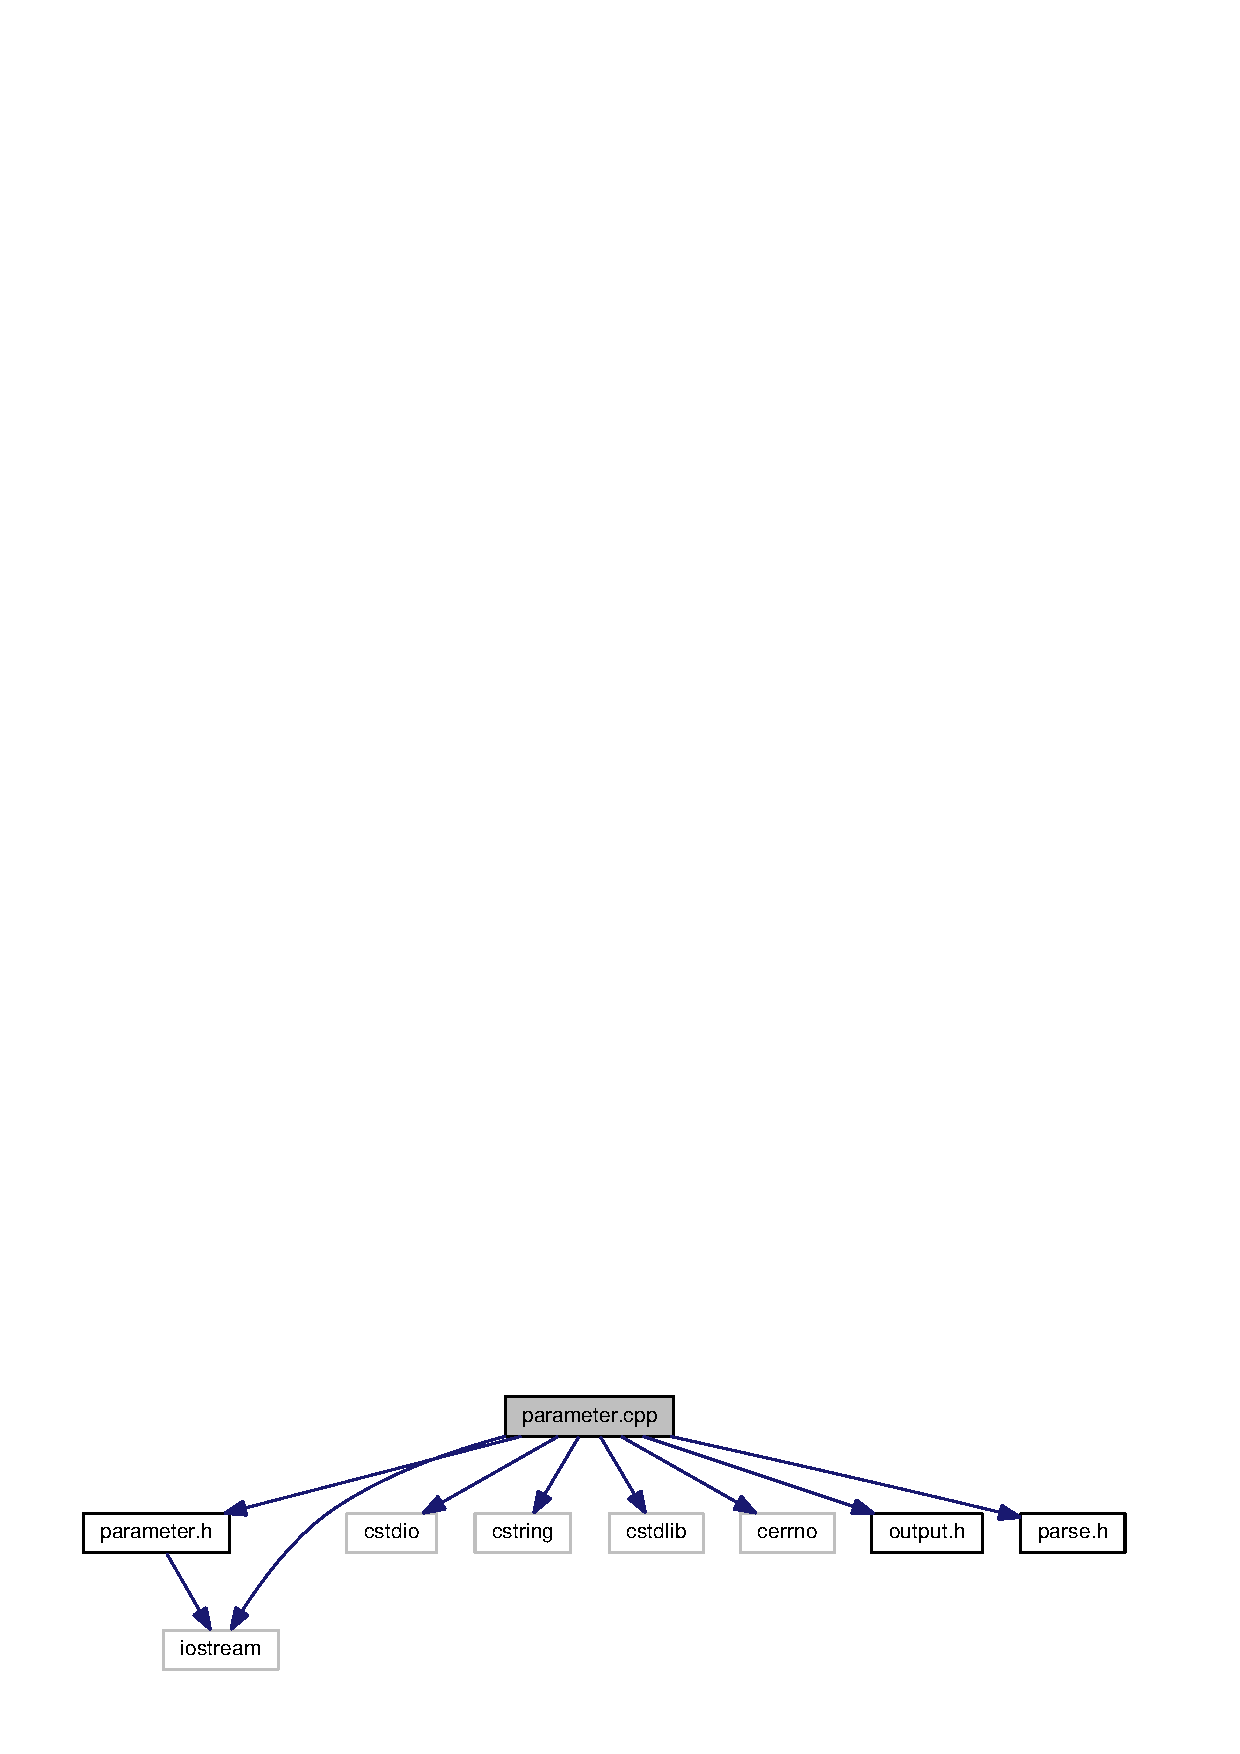
\includegraphics[width=350pt]{parameter_8cpp__incl}
\end{center}
\end{figure}
\subsection*{Functions}
\begin{DoxyCompactItemize}
\item 
const char $\ast$ {\bf sbool} (const bool \&p)
\item 
ostream \& {\bf operator$<$$<$} (ostream \&os, {\bf Parameter} \&p)
\end{DoxyCompactItemize}
\subsection*{Variables}
\begin{DoxyCompactItemize}
\item 
{\bf Parameter} {\bf par}
\end{DoxyCompactItemize}


\subsection{Function Documentation}
\index{parameter.\-cpp@{parameter.\-cpp}!operator$<$$<$@{operator$<$$<$}}
\index{operator$<$$<$@{operator$<$$<$}!parameter.cpp@{parameter.\-cpp}}
\subsubsection[{operator$<$$<$}]{\setlength{\rightskip}{0pt plus 5cm}ostream\& operator$<$$<$ (
\begin{DoxyParamCaption}
\item[{ostream \&}]{os, }
\item[{{\bf Parameter} \&}]{p}
\end{DoxyParamCaption}
)}\label{parameter_8cpp_acfe35248e4b79ab92dca7a80516b6ee9}


References Parameter\-::\-Write().

\index{parameter.\-cpp@{parameter.\-cpp}!sbool@{sbool}}
\index{sbool@{sbool}!parameter.cpp@{parameter.\-cpp}}
\subsubsection[{sbool}]{\setlength{\rightskip}{0pt plus 5cm}const char$\ast$ sbool (
\begin{DoxyParamCaption}
\item[{const bool \&}]{p}
\end{DoxyParamCaption}
)}\label{parameter_8cpp_a5f45a702ad254e252af17c1a81675af6}


Referenced by Parameter\-::\-Write().



\subsection{Variable Documentation}
\index{parameter.\-cpp@{parameter.\-cpp}!par@{par}}
\index{par@{par}!parameter.cpp@{parameter.\-cpp}}
\subsubsection[{par}]{\setlength{\rightskip}{0pt plus 5cm}{\bf Parameter} par}\label{parameter_8cpp_aa11a52593a908c20a7259a3e72c0b348}


Referenced by Info\-::\-Menu(), and Qt\-Graphics\-::\-Time\-Step\-Wrap().


\section{parameter.\-h File Reference}
\label{parameter_8h}\index{parameter.\-h@{parameter.\-h}}
{\ttfamily \#include $<$iostream$>$}\\*
Include dependency graph for parameter.\-h\-:
\nopagebreak
\begin{figure}[H]
\begin{center}
\leavevmode
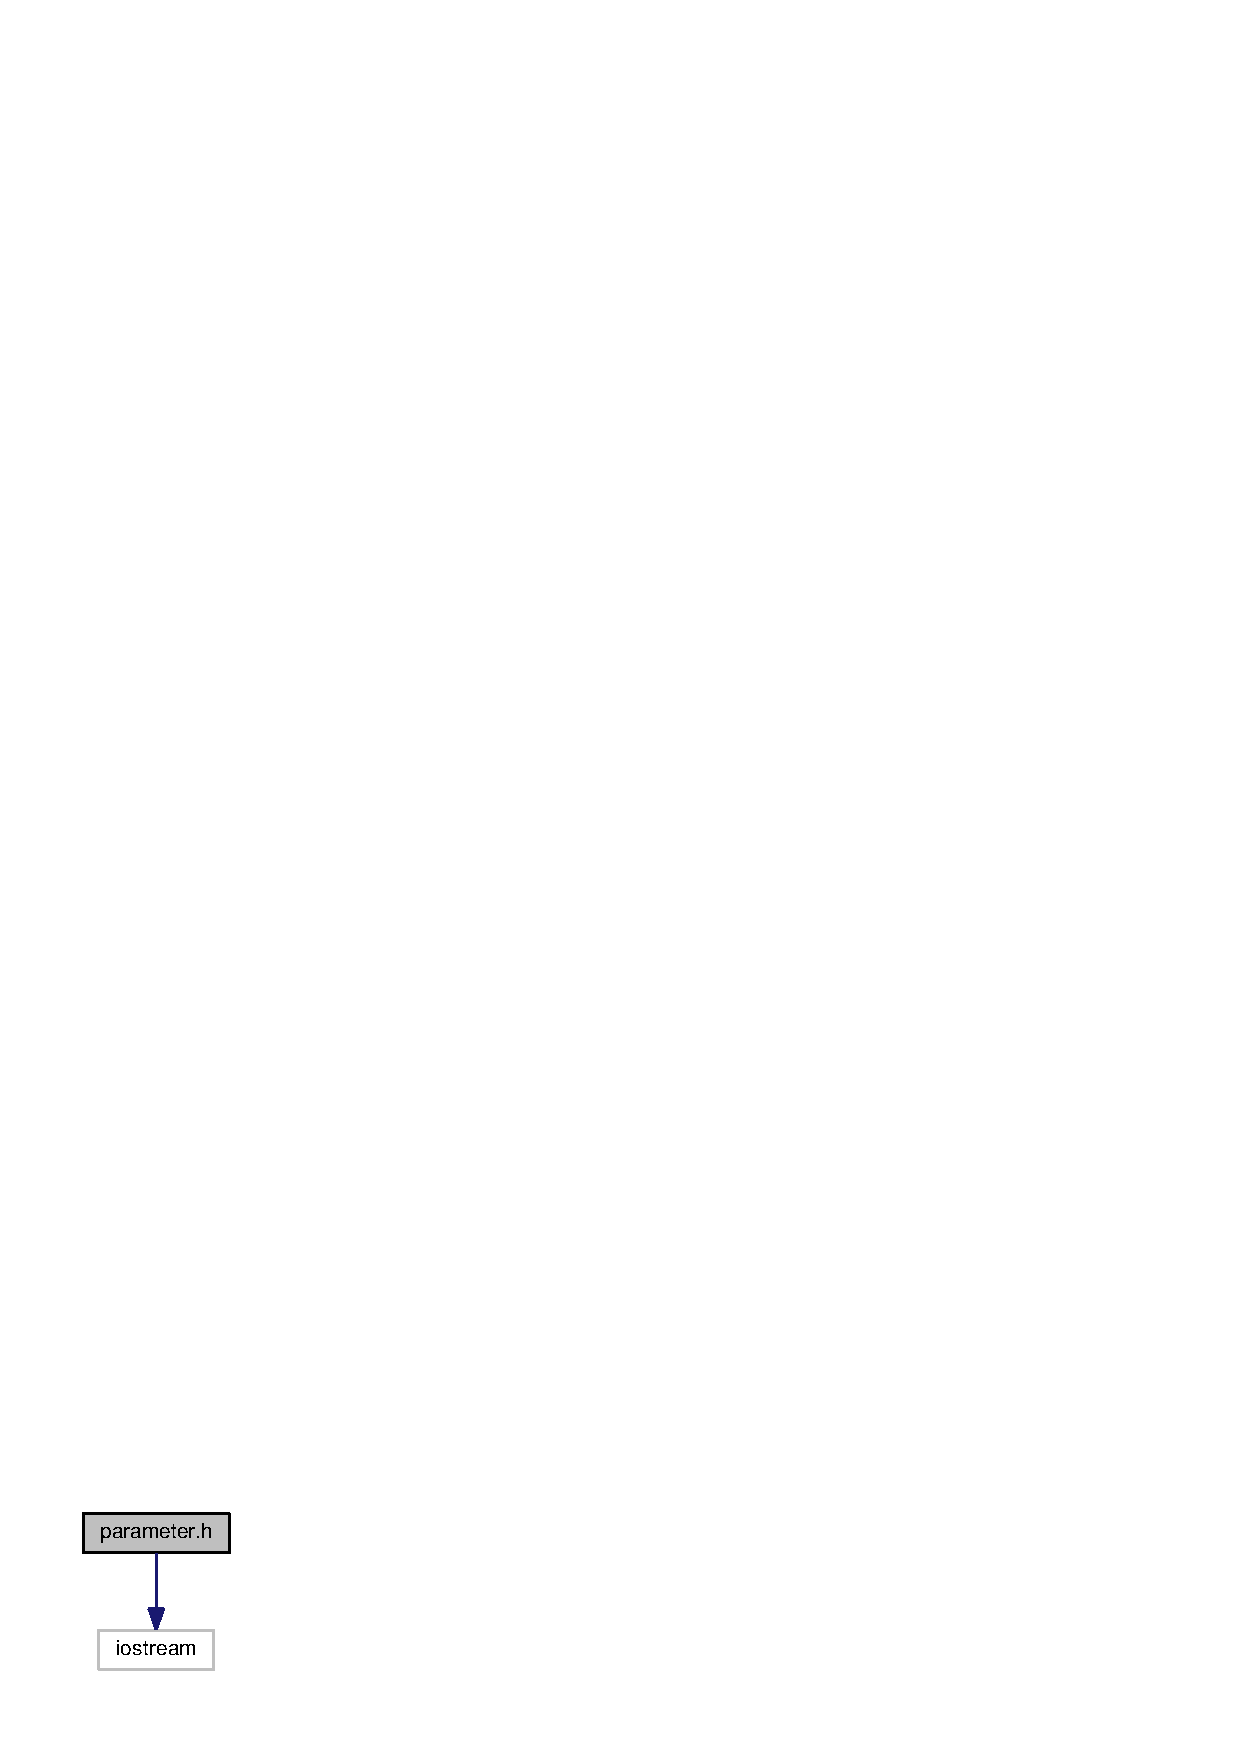
\includegraphics[width=114pt]{parameter_8h__incl}
\end{center}
\end{figure}
This graph shows which files directly or indirectly include this file\-:
\nopagebreak
\begin{figure}[H]
\begin{center}
\leavevmode
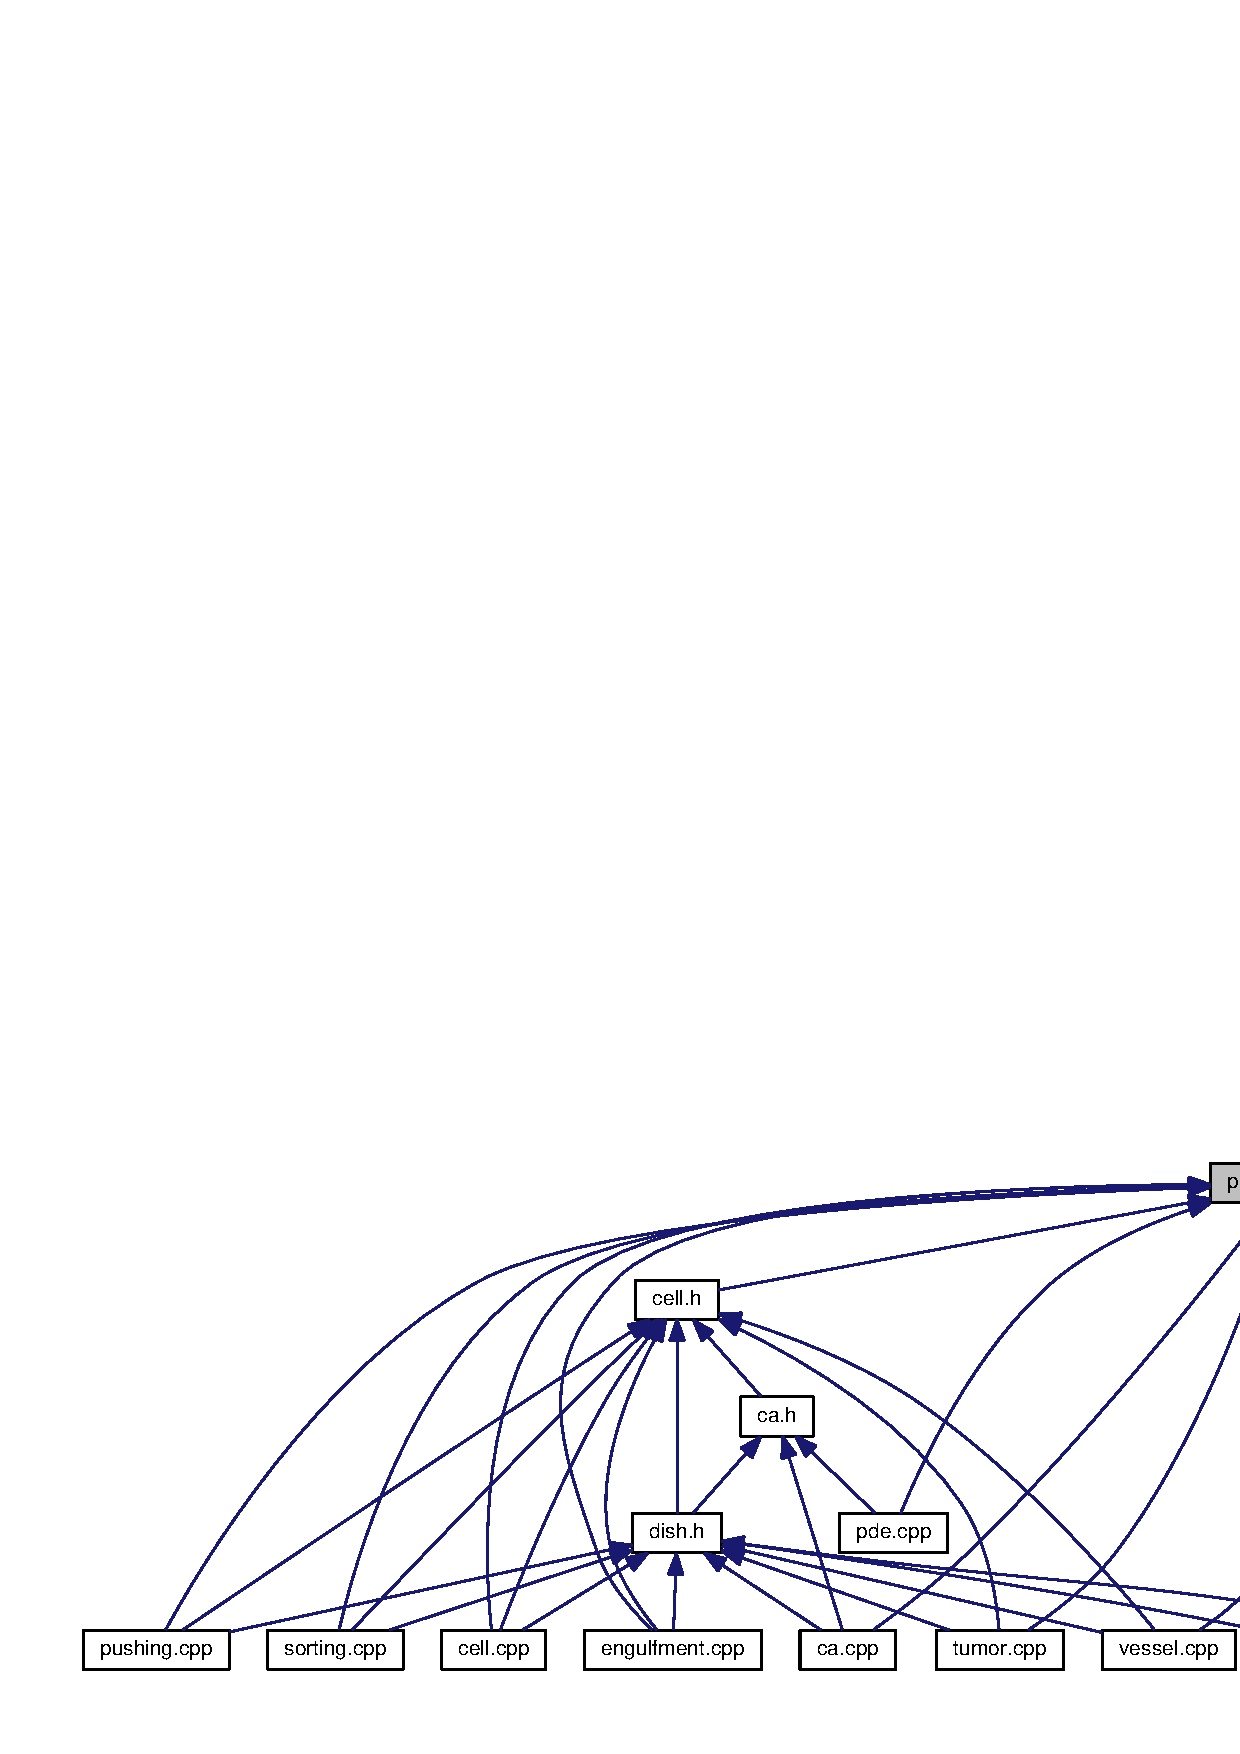
\includegraphics[width=350pt]{parameter_8h__dep__incl}
\end{center}
\end{figure}
\subsection*{Classes}
\begin{DoxyCompactItemize}
\item 
class {\bf Parameter}
\end{DoxyCompactItemize}
\subsection*{Functions}
\begin{DoxyCompactItemize}
\item 
ostream \& {\bf operator$<$$<$} (ostream \&os, {\bf Parameter} \&p)
\item 
const char $\ast$ {\bf sbool} (const bool \&p)
\end{DoxyCompactItemize}


\subsection{Function Documentation}
\index{parameter.\-h@{parameter.\-h}!operator$<$$<$@{operator$<$$<$}}
\index{operator$<$$<$@{operator$<$$<$}!parameter.h@{parameter.\-h}}
\subsubsection[{operator$<$$<$}]{\setlength{\rightskip}{0pt plus 5cm}ostream\& operator$<$$<$ (
\begin{DoxyParamCaption}
\item[{ostream \&}]{os, }
\item[{{\bf Parameter} \&}]{p}
\end{DoxyParamCaption}
)}\label{parameter_8h_acfe35248e4b79ab92dca7a80516b6ee9}


References Parameter\-::\-Write().

\index{parameter.\-h@{parameter.\-h}!sbool@{sbool}}
\index{sbool@{sbool}!parameter.h@{parameter.\-h}}
\subsubsection[{sbool}]{\setlength{\rightskip}{0pt plus 5cm}const char$\ast$ sbool (
\begin{DoxyParamCaption}
\item[{const bool \&}]{p}
\end{DoxyParamCaption}
)}\label{parameter_8h_a5f45a702ad254e252af17c1a81675af6}


Referenced by Parameter\-::\-Write().


\section{parse.\-cpp File Reference}
\label{parse_8cpp}\index{parse.\-cpp@{parse.\-cpp}}
{\ttfamily \#include $<$stdio.\-h$>$}\\*
{\ttfamily \#include $<$locale.\-h$>$}\\*
{\ttfamily \#include $<$string.\-h$>$}\\*
{\ttfamily \#include $<$stdlib.\-h$>$}\\*
{\ttfamily \#include $<$errno.\-h$>$}\\*
{\ttfamily \#include \char`\"{}warning.\-h\char`\"{}}\\*
{\ttfamily \#include \char`\"{}parse.\-h\char`\"{}}\\*
{\ttfamily \#include \char`\"{}output.\-h\char`\"{}}\\*
Include dependency graph for parse.\-cpp\-:
\nopagebreak
\begin{figure}[H]
\begin{center}
\leavevmode
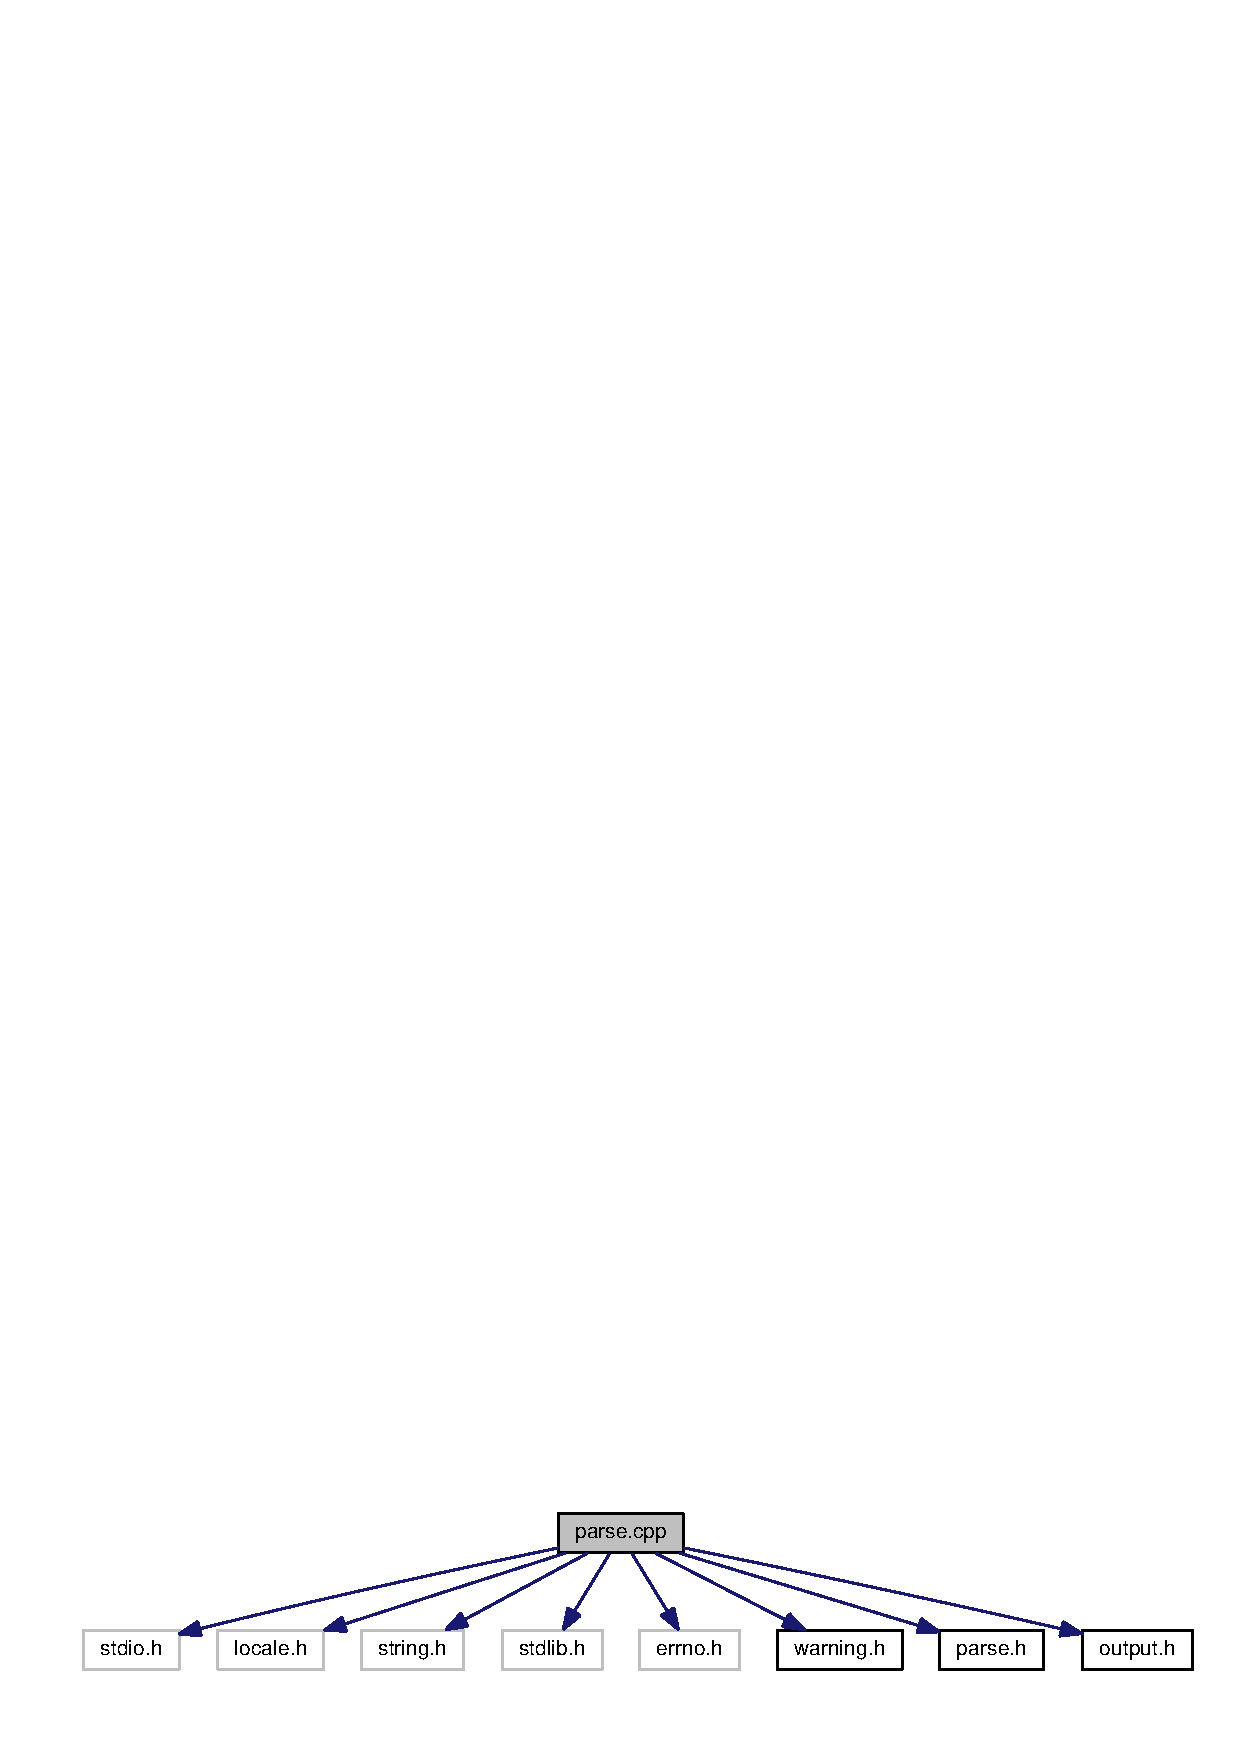
\includegraphics[width=350pt]{parse_8cpp__incl}
\end{center}
\end{figure}
\subsection*{Functions}
\begin{DoxyCompactItemize}
\item 
char $\ast$ {\bf Parse\-Par} (F\-I\-L\-E $\ast$fp, char $\ast$parameter, bool wrapflag)
\item 
int {\bf igetpar} (F\-I\-L\-E $\ast$fp, char $\ast$parameter, bool wrapflag)
\item 
int {\bf igetpar} (F\-I\-L\-E $\ast$fp, char $\ast$parameter, int default\-\_\-val, bool wrapflag)
\item 
float {\bf fgetpar} (F\-I\-L\-E $\ast$fp, char $\ast$parameter, bool wrapflag)
\item 
float {\bf fgetpar} (F\-I\-L\-E $\ast$fp, char $\ast$parameter, double default\-\_\-val, bool wrapflag)
\item 
double $\ast$ {\bf dgetparlist} (F\-I\-L\-E $\ast$fp, char $\ast$parameter, int n, bool wrapflag)
\item 
char $\ast$ {\bf sgetpar} (F\-I\-L\-E $\ast$fp, char $\ast$parameter, bool wrapflag)
\item 
char $\ast$ {\bf sgetpar} (F\-I\-L\-E $\ast$fp, char $\ast$parameter, const char $\ast$default\-\_\-val, bool wrapflag)
\item 
char $\ast$ {\bf bool\-\_\-str} (bool bool\-\_\-var)
\item 
bool {\bf bgetpar} (F\-I\-L\-E $\ast$fp, char $\ast$parameter, bool wrapflag)
\item 
bool {\bf bgetpar} (F\-I\-L\-E $\ast$fp, char $\ast$parameter, int default\-\_\-val, bool wrapflag)
\item 
char $\ast$ {\bf Search\-Token} (F\-I\-L\-E $\ast$fp, char $\ast$token, bool wrapflag)
\item 
int {\bf Token\-In\-Line\-P} (char $\ast$line, char $\ast$token)
\item 
void {\bf Skip\-Line} (F\-I\-L\-E $\ast$fp)
\item 
void {\bf Skip\-Token} (F\-I\-L\-E $\ast$fp, char $\ast$token, bool wrapflag)
\end{DoxyCompactItemize}


\subsection{Function Documentation}
\index{parse.\-cpp@{parse.\-cpp}!bgetpar@{bgetpar}}
\index{bgetpar@{bgetpar}!parse.cpp@{parse.\-cpp}}
\subsubsection[{bgetpar}]{\setlength{\rightskip}{0pt plus 5cm}bool bgetpar (
\begin{DoxyParamCaption}
\item[{F\-I\-L\-E $\ast$}]{fp, }
\item[{char $\ast$}]{parameter, }
\item[{bool}]{wrapflag}
\end{DoxyParamCaption}
)}\label{parse_8cpp_ac55ee6bfbd2cfd686c71efb955ce5a49}


References bgetpar().



Referenced by bgetpar(), and Parameter\-::\-Read().

\index{parse.\-cpp@{parse.\-cpp}!bgetpar@{bgetpar}}
\index{bgetpar@{bgetpar}!parse.cpp@{parse.\-cpp}}
\subsubsection[{bgetpar}]{\setlength{\rightskip}{0pt plus 5cm}bool bgetpar (
\begin{DoxyParamCaption}
\item[{F\-I\-L\-E $\ast$}]{fp, }
\item[{char $\ast$}]{parameter, }
\item[{int}]{default\-\_\-val, }
\item[{bool}]{wrapflag}
\end{DoxyParamCaption}
)}\label{parse_8cpp_a2daef242a27a1c9fda431bc30a1ecfd3}


References bool\-\_\-str(), error(), Parse\-Par(), and warning().

\index{parse.\-cpp@{parse.\-cpp}!bool\-\_\-str@{bool\-\_\-str}}
\index{bool\-\_\-str@{bool\-\_\-str}!parse.cpp@{parse.\-cpp}}
\subsubsection[{bool\-\_\-str}]{\setlength{\rightskip}{0pt plus 5cm}char$\ast$ bool\-\_\-str (
\begin{DoxyParamCaption}
\item[{bool}]{bool\-\_\-var}
\end{DoxyParamCaption}
)}\label{parse_8cpp_a2328592dbd8b961b0417eedc0056e6c7}


Referenced by bgetpar().

\index{parse.\-cpp@{parse.\-cpp}!dgetparlist@{dgetparlist}}
\index{dgetparlist@{dgetparlist}!parse.cpp@{parse.\-cpp}}
\subsubsection[{dgetparlist}]{\setlength{\rightskip}{0pt plus 5cm}double$\ast$ dgetparlist (
\begin{DoxyParamCaption}
\item[{F\-I\-L\-E $\ast$}]{fp, }
\item[{char $\ast$}]{parameter, }
\item[{int}]{n, }
\item[{bool}]{wrapflag}
\end{DoxyParamCaption}
)}\label{parse_8cpp_a5e164cf1271fc5d2dd578b12702f097a}


References error(), Parse\-Par(), and warning().



Referenced by Parameter\-::\-Read().

\index{parse.\-cpp@{parse.\-cpp}!fgetpar@{fgetpar}}
\index{fgetpar@{fgetpar}!parse.cpp@{parse.\-cpp}}
\subsubsection[{fgetpar}]{\setlength{\rightskip}{0pt plus 5cm}float fgetpar (
\begin{DoxyParamCaption}
\item[{F\-I\-L\-E $\ast$}]{fp, }
\item[{char $\ast$}]{parameter, }
\item[{bool}]{wrapflag}
\end{DoxyParamCaption}
)}\label{parse_8cpp_a2299c4462e8fba3b6c8b1c4294fe2a94}


References fgetpar().



Referenced by fgetpar(), and Parameter\-::\-Read().

\index{parse.\-cpp@{parse.\-cpp}!fgetpar@{fgetpar}}
\index{fgetpar@{fgetpar}!parse.cpp@{parse.\-cpp}}
\subsubsection[{fgetpar}]{\setlength{\rightskip}{0pt plus 5cm}float fgetpar (
\begin{DoxyParamCaption}
\item[{F\-I\-L\-E $\ast$}]{fp, }
\item[{char $\ast$}]{parameter, }
\item[{double}]{default\-\_\-val, }
\item[{bool}]{wrapflag}
\end{DoxyParamCaption}
)}\label{parse_8cpp_a890000bfc36a5f1e6c66ca098e1f8eb5}


References Parse\-Par(), and warning().

\index{parse.\-cpp@{parse.\-cpp}!igetpar@{igetpar}}
\index{igetpar@{igetpar}!parse.cpp@{parse.\-cpp}}
\subsubsection[{igetpar}]{\setlength{\rightskip}{0pt plus 5cm}int igetpar (
\begin{DoxyParamCaption}
\item[{F\-I\-L\-E $\ast$}]{fp, }
\item[{char $\ast$}]{parameter, }
\item[{bool}]{wrapflag}
\end{DoxyParamCaption}
)}\label{parse_8cpp_adf56eac548f104599e8a7cc51bf58aee}


References igetpar().



Referenced by igetpar(), and Parameter\-::\-Read().

\index{parse.\-cpp@{parse.\-cpp}!igetpar@{igetpar}}
\index{igetpar@{igetpar}!parse.cpp@{parse.\-cpp}}
\subsubsection[{igetpar}]{\setlength{\rightskip}{0pt plus 5cm}int igetpar (
\begin{DoxyParamCaption}
\item[{F\-I\-L\-E $\ast$}]{fp, }
\item[{char $\ast$}]{parameter, }
\item[{int}]{default\-\_\-val, }
\item[{bool}]{wrapflag}
\end{DoxyParamCaption}
)}\label{parse_8cpp_a6d3bbb1604d8f669171e426ac629a41d}


References Parse\-Par(), and warning().

\index{parse.\-cpp@{parse.\-cpp}!Parse\-Par@{Parse\-Par}}
\index{Parse\-Par@{Parse\-Par}!parse.cpp@{parse.\-cpp}}
\subsubsection[{Parse\-Par}]{\setlength{\rightskip}{0pt plus 5cm}char$\ast$ Parse\-Par (
\begin{DoxyParamCaption}
\item[{F\-I\-L\-E $\ast$}]{fp, }
\item[{char $\ast$}]{parameter, }
\item[{bool}]{wrapflag}
\end{DoxyParamCaption}
)}\label{parse_8cpp_ad7e24aa69d628788949f9ac9b0474e1c}


References error(), Search\-Token(), and warning().



Referenced by bgetpar(), dgetparlist(), fgetpar(), igetpar(), and sgetpar().

\index{parse.\-cpp@{parse.\-cpp}!Search\-Token@{Search\-Token}}
\index{Search\-Token@{Search\-Token}!parse.cpp@{parse.\-cpp}}
\subsubsection[{Search\-Token}]{\setlength{\rightskip}{0pt plus 5cm}char$\ast$ Search\-Token (
\begin{DoxyParamCaption}
\item[{F\-I\-L\-E $\ast$}]{fp, }
\item[{char $\ast$}]{token, }
\item[{bool}]{wrapflag}
\end{DoxyParamCaption}
)}\label{parse_8cpp_a1446df70c82e543b3e786d17b4105a3a}


References errno, error(), Read\-Line(), and warning().



Referenced by Parse\-Par(), and Skip\-Token().

\index{parse.\-cpp@{parse.\-cpp}!sgetpar@{sgetpar}}
\index{sgetpar@{sgetpar}!parse.cpp@{parse.\-cpp}}
\subsubsection[{sgetpar}]{\setlength{\rightskip}{0pt plus 5cm}char$\ast$ sgetpar (
\begin{DoxyParamCaption}
\item[{F\-I\-L\-E $\ast$}]{fp, }
\item[{char $\ast$}]{parameter, }
\item[{bool}]{wrapflag}
\end{DoxyParamCaption}
)}\label{parse_8cpp_adbecbe0b887fa03998389764e0394400}


References sgetpar().



Referenced by Parameter\-::\-Read(), and sgetpar().

\index{parse.\-cpp@{parse.\-cpp}!sgetpar@{sgetpar}}
\index{sgetpar@{sgetpar}!parse.cpp@{parse.\-cpp}}
\subsubsection[{sgetpar}]{\setlength{\rightskip}{0pt plus 5cm}char$\ast$ sgetpar (
\begin{DoxyParamCaption}
\item[{F\-I\-L\-E $\ast$}]{fp, }
\item[{char $\ast$}]{parameter, }
\item[{const char $\ast$}]{default\-\_\-val, }
\item[{bool}]{wrapflag}
\end{DoxyParamCaption}
)}\label{parse_8cpp_afd8452193c8594b6e97191174c12f63c}


References Parse\-Par(), and warning().

\index{parse.\-cpp@{parse.\-cpp}!Skip\-Line@{Skip\-Line}}
\index{Skip\-Line@{Skip\-Line}!parse.cpp@{parse.\-cpp}}
\subsubsection[{Skip\-Line}]{\setlength{\rightskip}{0pt plus 5cm}void Skip\-Line (
\begin{DoxyParamCaption}
\item[{F\-I\-L\-E $\ast$}]{fp}
\end{DoxyParamCaption}
)}\label{parse_8cpp_af032c357bf5040759c3a57073182be95}


References Read\-Line().

\index{parse.\-cpp@{parse.\-cpp}!Skip\-Token@{Skip\-Token}}
\index{Skip\-Token@{Skip\-Token}!parse.cpp@{parse.\-cpp}}
\subsubsection[{Skip\-Token}]{\setlength{\rightskip}{0pt plus 5cm}void Skip\-Token (
\begin{DoxyParamCaption}
\item[{F\-I\-L\-E $\ast$}]{fp, }
\item[{char $\ast$}]{token, }
\item[{bool}]{wrapflag}
\end{DoxyParamCaption}
)}\label{parse_8cpp_afc42a9f3ab59e8d07161aa1e2c9cbe83}


References error(), and Search\-Token().

\index{parse.\-cpp@{parse.\-cpp}!Token\-In\-Line\-P@{Token\-In\-Line\-P}}
\index{Token\-In\-Line\-P@{Token\-In\-Line\-P}!parse.cpp@{parse.\-cpp}}
\subsubsection[{Token\-In\-Line\-P}]{\setlength{\rightskip}{0pt plus 5cm}int Token\-In\-Line\-P (
\begin{DoxyParamCaption}
\item[{char $\ast$}]{line, }
\item[{char $\ast$}]{token}
\end{DoxyParamCaption}
)}\label{parse_8cpp_abc93274aa269efda64082d0a90cb32cf}

\section{parse.\-h File Reference}
\label{parse_8h}\index{parse.\-h@{parse.\-h}}
This graph shows which files directly or indirectly include this file\-:
\nopagebreak
\begin{figure}[H]
\begin{center}
\leavevmode
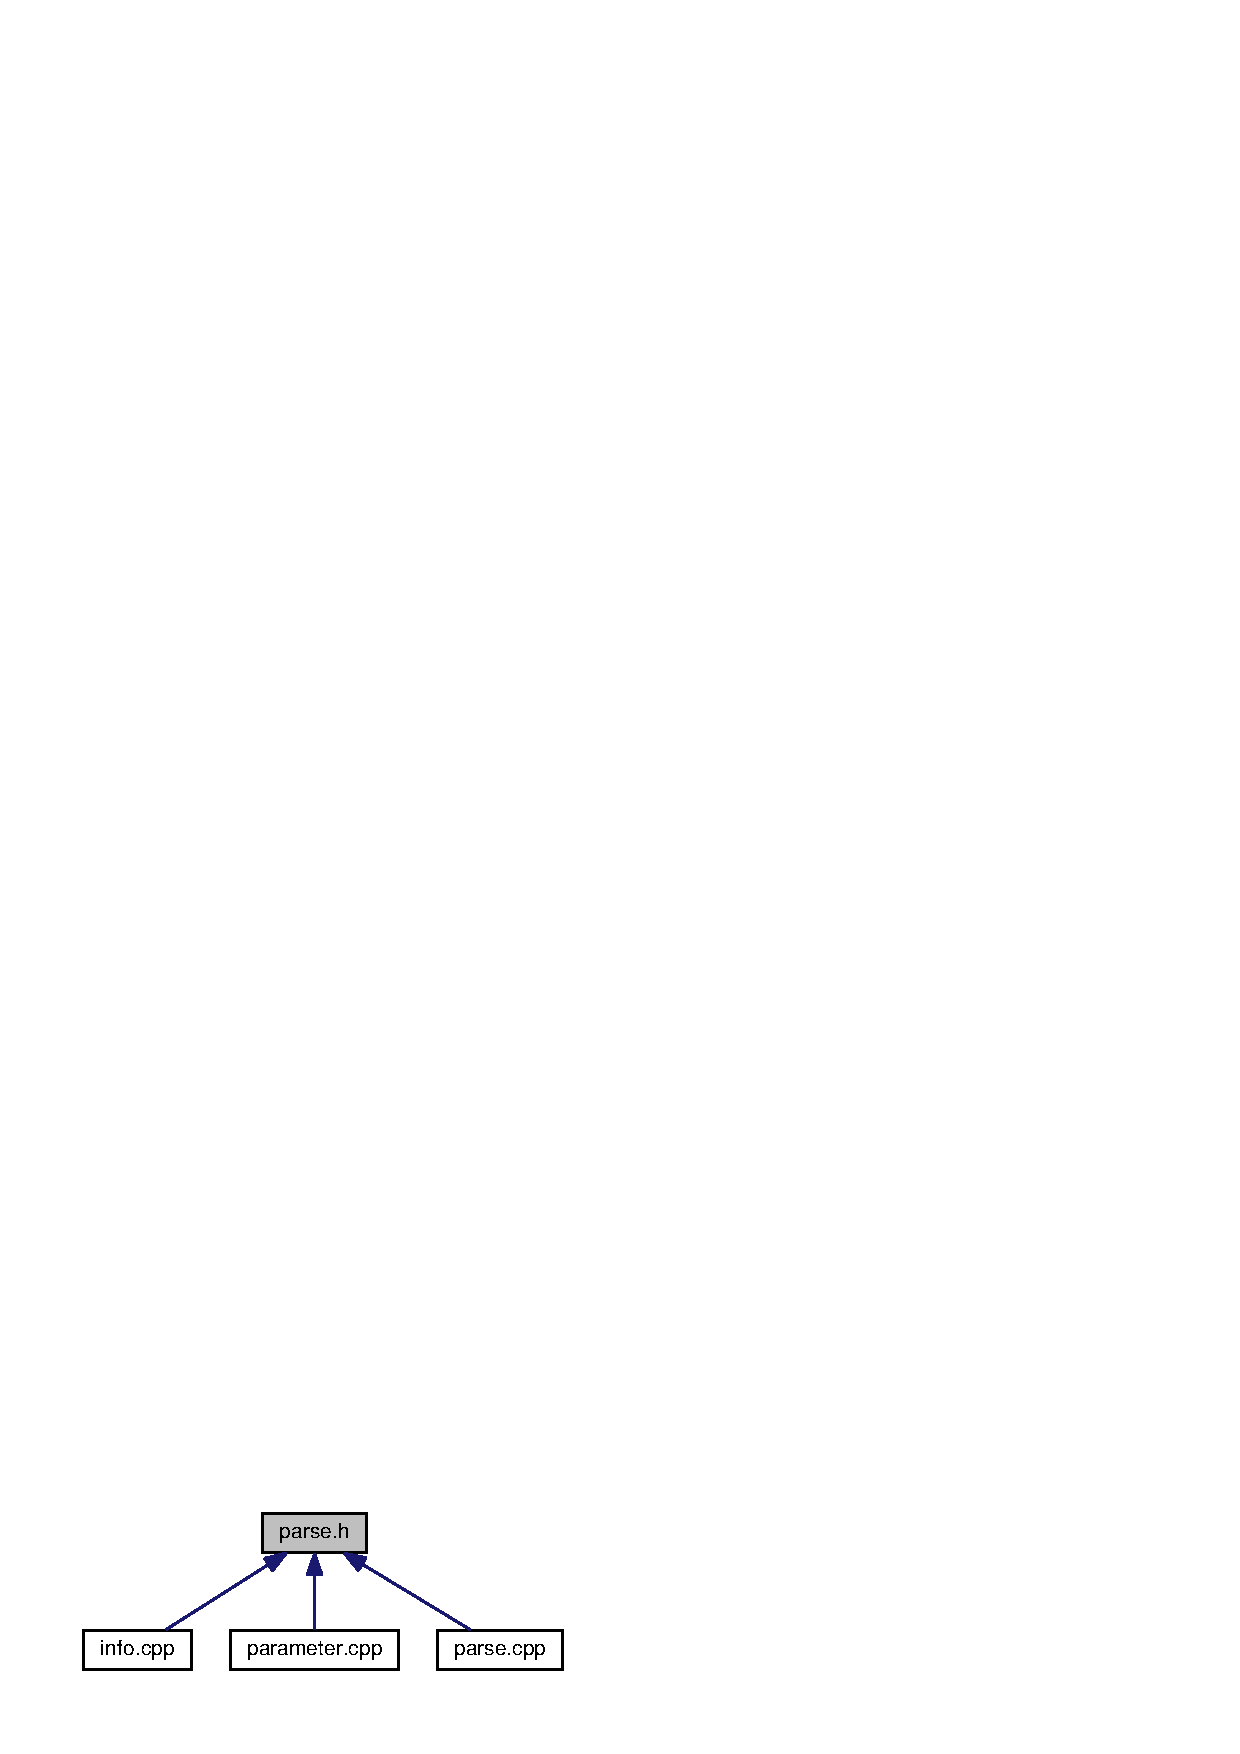
\includegraphics[width=274pt]{parse_8h__dep__incl}
\end{center}
\end{figure}
\subsection*{Functions}
\begin{DoxyCompactItemize}
\item 
char $\ast$ {\bf Parse\-Par} (F\-I\-L\-E $\ast$fp, char $\ast$parameter, bool wrapflag)
\item 
int {\bf igetpar} (F\-I\-L\-E $\ast$fp, char $\ast$parameter, bool wrapflag)
\item 
int {\bf igetpar} (F\-I\-L\-E $\ast$fp, char $\ast$parameter, int default\-\_\-val, bool wrapflag)
\item 
float {\bf fgetpar} (F\-I\-L\-E $\ast$fp, char $\ast$parameter, bool wrapflag)
\item 
float {\bf fgetpar} (F\-I\-L\-E $\ast$fp, char $\ast$parameter, double default\-\_\-val, bool wrapflag)
\item 
double $\ast$ {\bf dgetparlist} (F\-I\-L\-E $\ast$fp, char $\ast$parameter, int n, bool wrapflag)
\item 
char $\ast$ {\bf sgetpar} (F\-I\-L\-E $\ast$fp, char $\ast$parameter, bool wrapflag)
\item 
char $\ast$ {\bf sgetpar} (F\-I\-L\-E $\ast$fp, char $\ast$parameter, const char $\ast$default\-\_\-val, bool wrapflag)
\item 
bool {\bf bgetpar} (F\-I\-L\-E $\ast$fp, char $\ast$parameter, bool wrapflag)
\item 
bool {\bf bgetpar} (F\-I\-L\-E $\ast$fp, char $\ast$parameter, int default\-\_\-val, bool wrapflag)
\item 
char $\ast$ {\bf Search\-Token} (F\-I\-L\-E $\ast$fp, char $\ast$token, bool wrapflag)
\item 
int {\bf Token\-In\-Line\-P} (char $\ast$line, char $\ast$token)
\item 
void {\bf Skip\-Token} (F\-I\-L\-E $\ast$fp, char $\ast$token, bool wrapflag)
\item 
void {\bf Skip\-Line} (F\-I\-L\-E $\ast$fp)
\item 
char $\ast$ {\bf bool\-\_\-str} (bool bool\-\_\-var)
\end{DoxyCompactItemize}


\subsection{Function Documentation}
\index{parse.\-h@{parse.\-h}!bgetpar@{bgetpar}}
\index{bgetpar@{bgetpar}!parse.h@{parse.\-h}}
\subsubsection[{bgetpar}]{\setlength{\rightskip}{0pt plus 5cm}bool bgetpar (
\begin{DoxyParamCaption}
\item[{F\-I\-L\-E $\ast$}]{fp, }
\item[{char $\ast$}]{parameter, }
\item[{bool}]{wrapflag}
\end{DoxyParamCaption}
)}\label{parse_8h_ac55ee6bfbd2cfd686c71efb955ce5a49}


References bgetpar().



Referenced by bgetpar(), and Parameter\-::\-Read().

\index{parse.\-h@{parse.\-h}!bgetpar@{bgetpar}}
\index{bgetpar@{bgetpar}!parse.h@{parse.\-h}}
\subsubsection[{bgetpar}]{\setlength{\rightskip}{0pt plus 5cm}bool bgetpar (
\begin{DoxyParamCaption}
\item[{F\-I\-L\-E $\ast$}]{fp, }
\item[{char $\ast$}]{parameter, }
\item[{int}]{default\-\_\-val, }
\item[{bool}]{wrapflag}
\end{DoxyParamCaption}
)}\label{parse_8h_a2daef242a27a1c9fda431bc30a1ecfd3}


References bool\-\_\-str(), error(), Parse\-Par(), and warning().

\index{parse.\-h@{parse.\-h}!bool\-\_\-str@{bool\-\_\-str}}
\index{bool\-\_\-str@{bool\-\_\-str}!parse.h@{parse.\-h}}
\subsubsection[{bool\-\_\-str}]{\setlength{\rightskip}{0pt plus 5cm}char$\ast$ bool\-\_\-str (
\begin{DoxyParamCaption}
\item[{bool}]{bool\-\_\-var}
\end{DoxyParamCaption}
)}\label{parse_8h_a2328592dbd8b961b0417eedc0056e6c7}


Referenced by bgetpar().

\index{parse.\-h@{parse.\-h}!dgetparlist@{dgetparlist}}
\index{dgetparlist@{dgetparlist}!parse.h@{parse.\-h}}
\subsubsection[{dgetparlist}]{\setlength{\rightskip}{0pt plus 5cm}double$\ast$ dgetparlist (
\begin{DoxyParamCaption}
\item[{F\-I\-L\-E $\ast$}]{fp, }
\item[{char $\ast$}]{parameter, }
\item[{int}]{n, }
\item[{bool}]{wrapflag}
\end{DoxyParamCaption}
)}\label{parse_8h_a5e164cf1271fc5d2dd578b12702f097a}


References error(), Parse\-Par(), and warning().



Referenced by Parameter\-::\-Read().

\index{parse.\-h@{parse.\-h}!fgetpar@{fgetpar}}
\index{fgetpar@{fgetpar}!parse.h@{parse.\-h}}
\subsubsection[{fgetpar}]{\setlength{\rightskip}{0pt plus 5cm}float fgetpar (
\begin{DoxyParamCaption}
\item[{F\-I\-L\-E $\ast$}]{fp, }
\item[{char $\ast$}]{parameter, }
\item[{bool}]{wrapflag}
\end{DoxyParamCaption}
)}\label{parse_8h_a2299c4462e8fba3b6c8b1c4294fe2a94}


References fgetpar().



Referenced by fgetpar(), and Parameter\-::\-Read().

\index{parse.\-h@{parse.\-h}!fgetpar@{fgetpar}}
\index{fgetpar@{fgetpar}!parse.h@{parse.\-h}}
\subsubsection[{fgetpar}]{\setlength{\rightskip}{0pt plus 5cm}float fgetpar (
\begin{DoxyParamCaption}
\item[{F\-I\-L\-E $\ast$}]{fp, }
\item[{char $\ast$}]{parameter, }
\item[{double}]{default\-\_\-val, }
\item[{bool}]{wrapflag}
\end{DoxyParamCaption}
)}\label{parse_8h_a890000bfc36a5f1e6c66ca098e1f8eb5}


References Parse\-Par(), and warning().

\index{parse.\-h@{parse.\-h}!igetpar@{igetpar}}
\index{igetpar@{igetpar}!parse.h@{parse.\-h}}
\subsubsection[{igetpar}]{\setlength{\rightskip}{0pt plus 5cm}int igetpar (
\begin{DoxyParamCaption}
\item[{F\-I\-L\-E $\ast$}]{fp, }
\item[{char $\ast$}]{parameter, }
\item[{bool}]{wrapflag}
\end{DoxyParamCaption}
)}\label{parse_8h_adf56eac548f104599e8a7cc51bf58aee}


References igetpar().



Referenced by igetpar(), and Parameter\-::\-Read().

\index{parse.\-h@{parse.\-h}!igetpar@{igetpar}}
\index{igetpar@{igetpar}!parse.h@{parse.\-h}}
\subsubsection[{igetpar}]{\setlength{\rightskip}{0pt plus 5cm}int igetpar (
\begin{DoxyParamCaption}
\item[{F\-I\-L\-E $\ast$}]{fp, }
\item[{char $\ast$}]{parameter, }
\item[{int}]{default\-\_\-val, }
\item[{bool}]{wrapflag}
\end{DoxyParamCaption}
)}\label{parse_8h_a6d3bbb1604d8f669171e426ac629a41d}


References Parse\-Par(), and warning().

\index{parse.\-h@{parse.\-h}!Parse\-Par@{Parse\-Par}}
\index{Parse\-Par@{Parse\-Par}!parse.h@{parse.\-h}}
\subsubsection[{Parse\-Par}]{\setlength{\rightskip}{0pt plus 5cm}char$\ast$ Parse\-Par (
\begin{DoxyParamCaption}
\item[{F\-I\-L\-E $\ast$}]{fp, }
\item[{char $\ast$}]{parameter, }
\item[{bool}]{wrapflag}
\end{DoxyParamCaption}
)}\label{parse_8h_ad7e24aa69d628788949f9ac9b0474e1c}


References error(), Search\-Token(), and warning().



Referenced by bgetpar(), dgetparlist(), fgetpar(), igetpar(), and sgetpar().

\index{parse.\-h@{parse.\-h}!Search\-Token@{Search\-Token}}
\index{Search\-Token@{Search\-Token}!parse.h@{parse.\-h}}
\subsubsection[{Search\-Token}]{\setlength{\rightskip}{0pt plus 5cm}char$\ast$ Search\-Token (
\begin{DoxyParamCaption}
\item[{F\-I\-L\-E $\ast$}]{fp, }
\item[{char $\ast$}]{token, }
\item[{bool}]{wrapflag}
\end{DoxyParamCaption}
)}\label{parse_8h_a1446df70c82e543b3e786d17b4105a3a}


References errno, error(), Read\-Line(), and warning().



Referenced by Parse\-Par(), and Skip\-Token().

\index{parse.\-h@{parse.\-h}!sgetpar@{sgetpar}}
\index{sgetpar@{sgetpar}!parse.h@{parse.\-h}}
\subsubsection[{sgetpar}]{\setlength{\rightskip}{0pt plus 5cm}char$\ast$ sgetpar (
\begin{DoxyParamCaption}
\item[{F\-I\-L\-E $\ast$}]{fp, }
\item[{char $\ast$}]{parameter, }
\item[{bool}]{wrapflag}
\end{DoxyParamCaption}
)}\label{parse_8h_adbecbe0b887fa03998389764e0394400}


References sgetpar().



Referenced by Parameter\-::\-Read(), and sgetpar().

\index{parse.\-h@{parse.\-h}!sgetpar@{sgetpar}}
\index{sgetpar@{sgetpar}!parse.h@{parse.\-h}}
\subsubsection[{sgetpar}]{\setlength{\rightskip}{0pt plus 5cm}char$\ast$ sgetpar (
\begin{DoxyParamCaption}
\item[{F\-I\-L\-E $\ast$}]{fp, }
\item[{char $\ast$}]{parameter, }
\item[{const char $\ast$}]{default\-\_\-val, }
\item[{bool}]{wrapflag}
\end{DoxyParamCaption}
)}\label{parse_8h_afd8452193c8594b6e97191174c12f63c}


References Parse\-Par(), and warning().

\index{parse.\-h@{parse.\-h}!Skip\-Line@{Skip\-Line}}
\index{Skip\-Line@{Skip\-Line}!parse.h@{parse.\-h}}
\subsubsection[{Skip\-Line}]{\setlength{\rightskip}{0pt plus 5cm}void Skip\-Line (
\begin{DoxyParamCaption}
\item[{F\-I\-L\-E $\ast$}]{fp}
\end{DoxyParamCaption}
)}\label{parse_8h_af032c357bf5040759c3a57073182be95}


References Read\-Line().

\index{parse.\-h@{parse.\-h}!Skip\-Token@{Skip\-Token}}
\index{Skip\-Token@{Skip\-Token}!parse.h@{parse.\-h}}
\subsubsection[{Skip\-Token}]{\setlength{\rightskip}{0pt plus 5cm}void Skip\-Token (
\begin{DoxyParamCaption}
\item[{F\-I\-L\-E $\ast$}]{fp, }
\item[{char $\ast$}]{token, }
\item[{bool}]{wrapflag}
\end{DoxyParamCaption}
)}\label{parse_8h_afc42a9f3ab59e8d07161aa1e2c9cbe83}


References error(), and Search\-Token().

\index{parse.\-h@{parse.\-h}!Token\-In\-Line\-P@{Token\-In\-Line\-P}}
\index{Token\-In\-Line\-P@{Token\-In\-Line\-P}!parse.h@{parse.\-h}}
\subsubsection[{Token\-In\-Line\-P}]{\setlength{\rightskip}{0pt plus 5cm}int Token\-In\-Line\-P (
\begin{DoxyParamCaption}
\item[{char $\ast$}]{line, }
\item[{char $\ast$}]{token}
\end{DoxyParamCaption}
)}\label{parse_8h_abc93274aa269efda64082d0a90cb32cf}

\section{pde.\-cpp File Reference}
\label{pde_8cpp}\index{pde.\-cpp@{pde.\-cpp}}
{\ttfamily \#include $<$stdio.\-h$>$}\\*
{\ttfamily \#include $<$math.\-h$>$}\\*
{\ttfamily \#include $<$cstdlib$>$}\\*
{\ttfamily \#include \char`\"{}crash.\-h\char`\"{}}\\*
{\ttfamily \#include \char`\"{}parameter.\-h\char`\"{}}\\*
{\ttfamily \#include \char`\"{}ca.\-h\char`\"{}}\\*
{\ttfamily \#include \char`\"{}pde.\-h\char`\"{}}\\*
{\ttfamily \#include \char`\"{}conrec.\-h\char`\"{}}\\*
Include dependency graph for pde.\-cpp\-:
\nopagebreak
\begin{figure}[H]
\begin{center}
\leavevmode
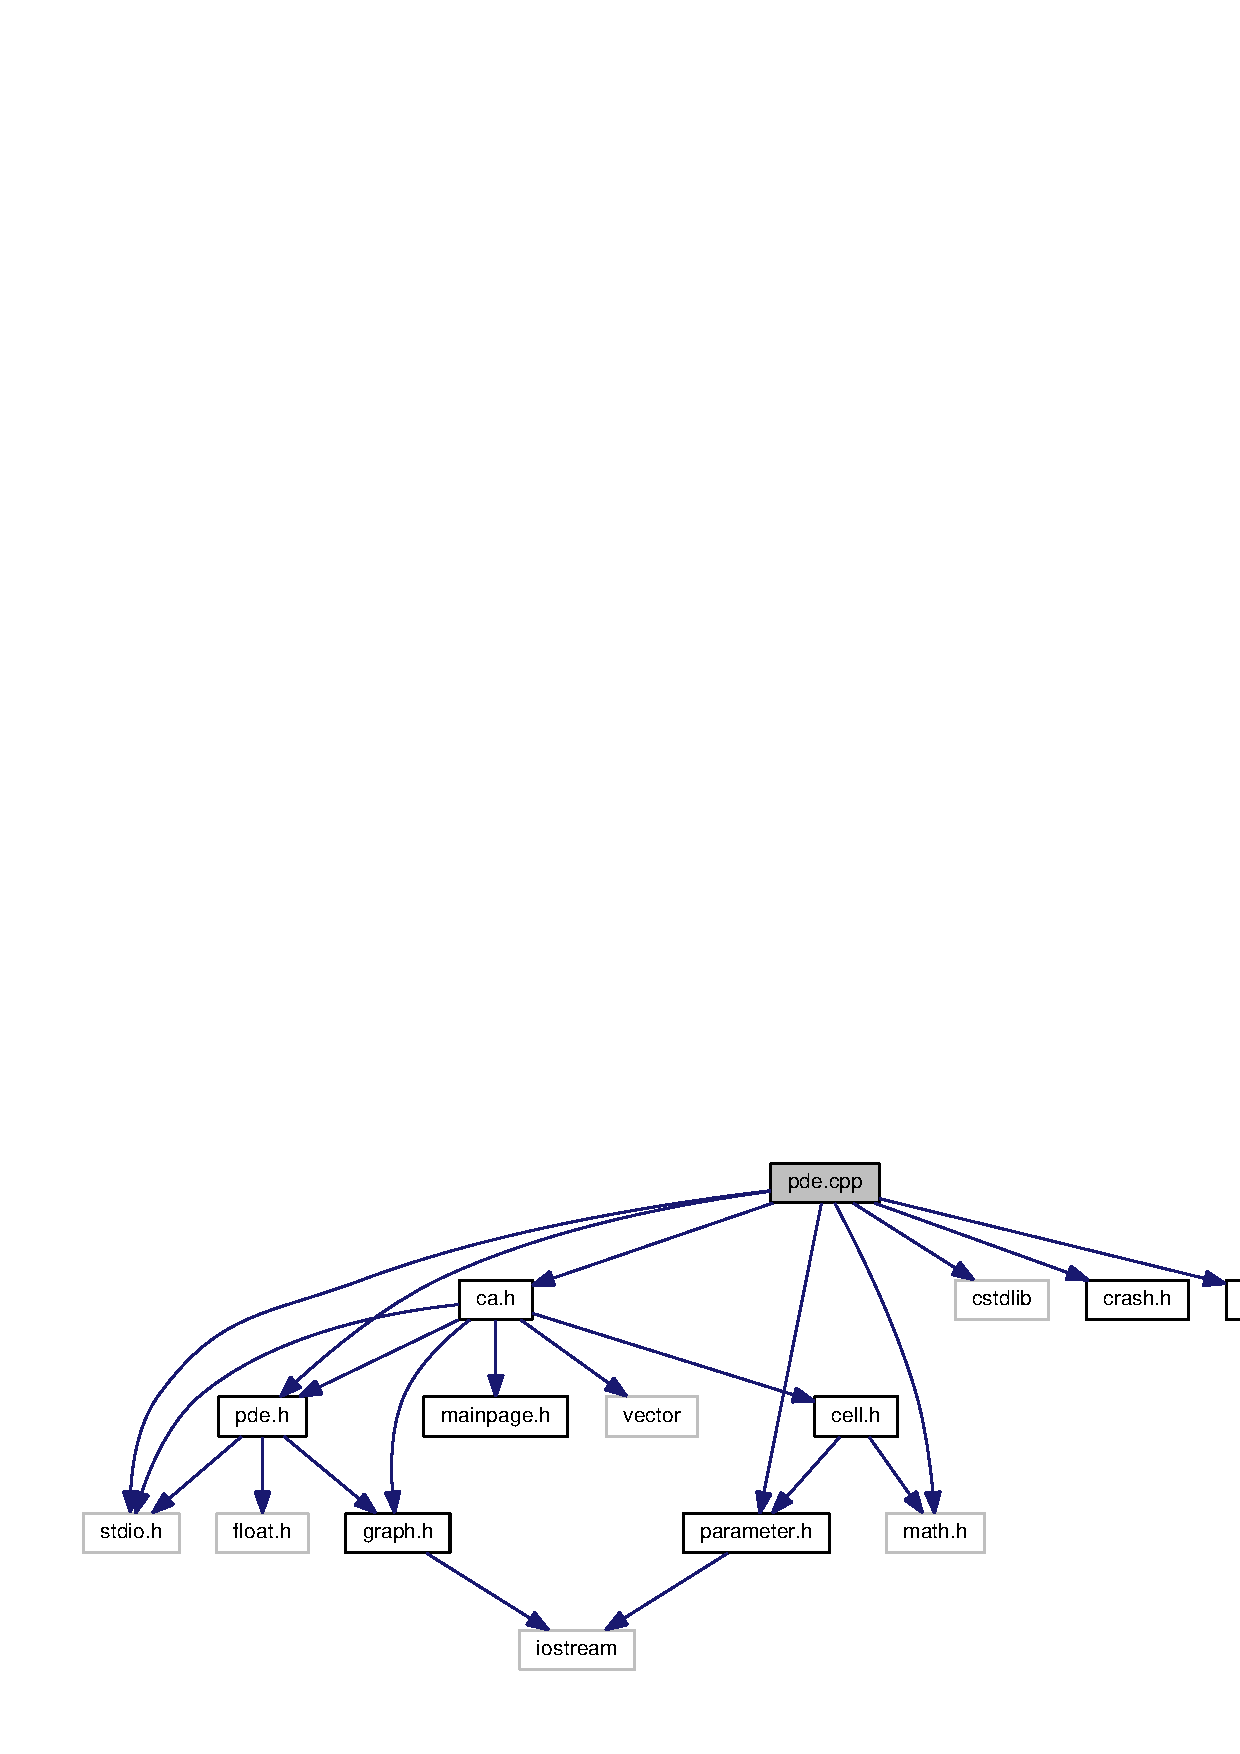
\includegraphics[width=350pt]{pde_8cpp__incl}
\end{center}
\end{figure}
\subsection*{Variables}
\begin{DoxyCompactItemize}
\item 
{\bf Parameter} {\bf par}
\end{DoxyCompactItemize}


\subsection{Variable Documentation}
\index{pde.\-cpp@{pde.\-cpp}!par@{par}}
\index{par@{par}!pde.cpp@{pde.\-cpp}}
\subsubsection[{par}]{\setlength{\rightskip}{0pt plus 5cm}{\bf Parameter} par}\label{pde_8cpp_aa11a52593a908c20a7259a3e72c0b348}

\section{pde.\-h File Reference}
\label{pde_8h}\index{pde.\-h@{pde.\-h}}
{\ttfamily \#include $<$stdio.\-h$>$}\\*
{\ttfamily \#include $<$float.\-h$>$}\\*
{\ttfamily \#include \char`\"{}graph.\-h\char`\"{}}\\*
Include dependency graph for pde.\-h\-:
\nopagebreak
\begin{figure}[H]
\begin{center}
\leavevmode
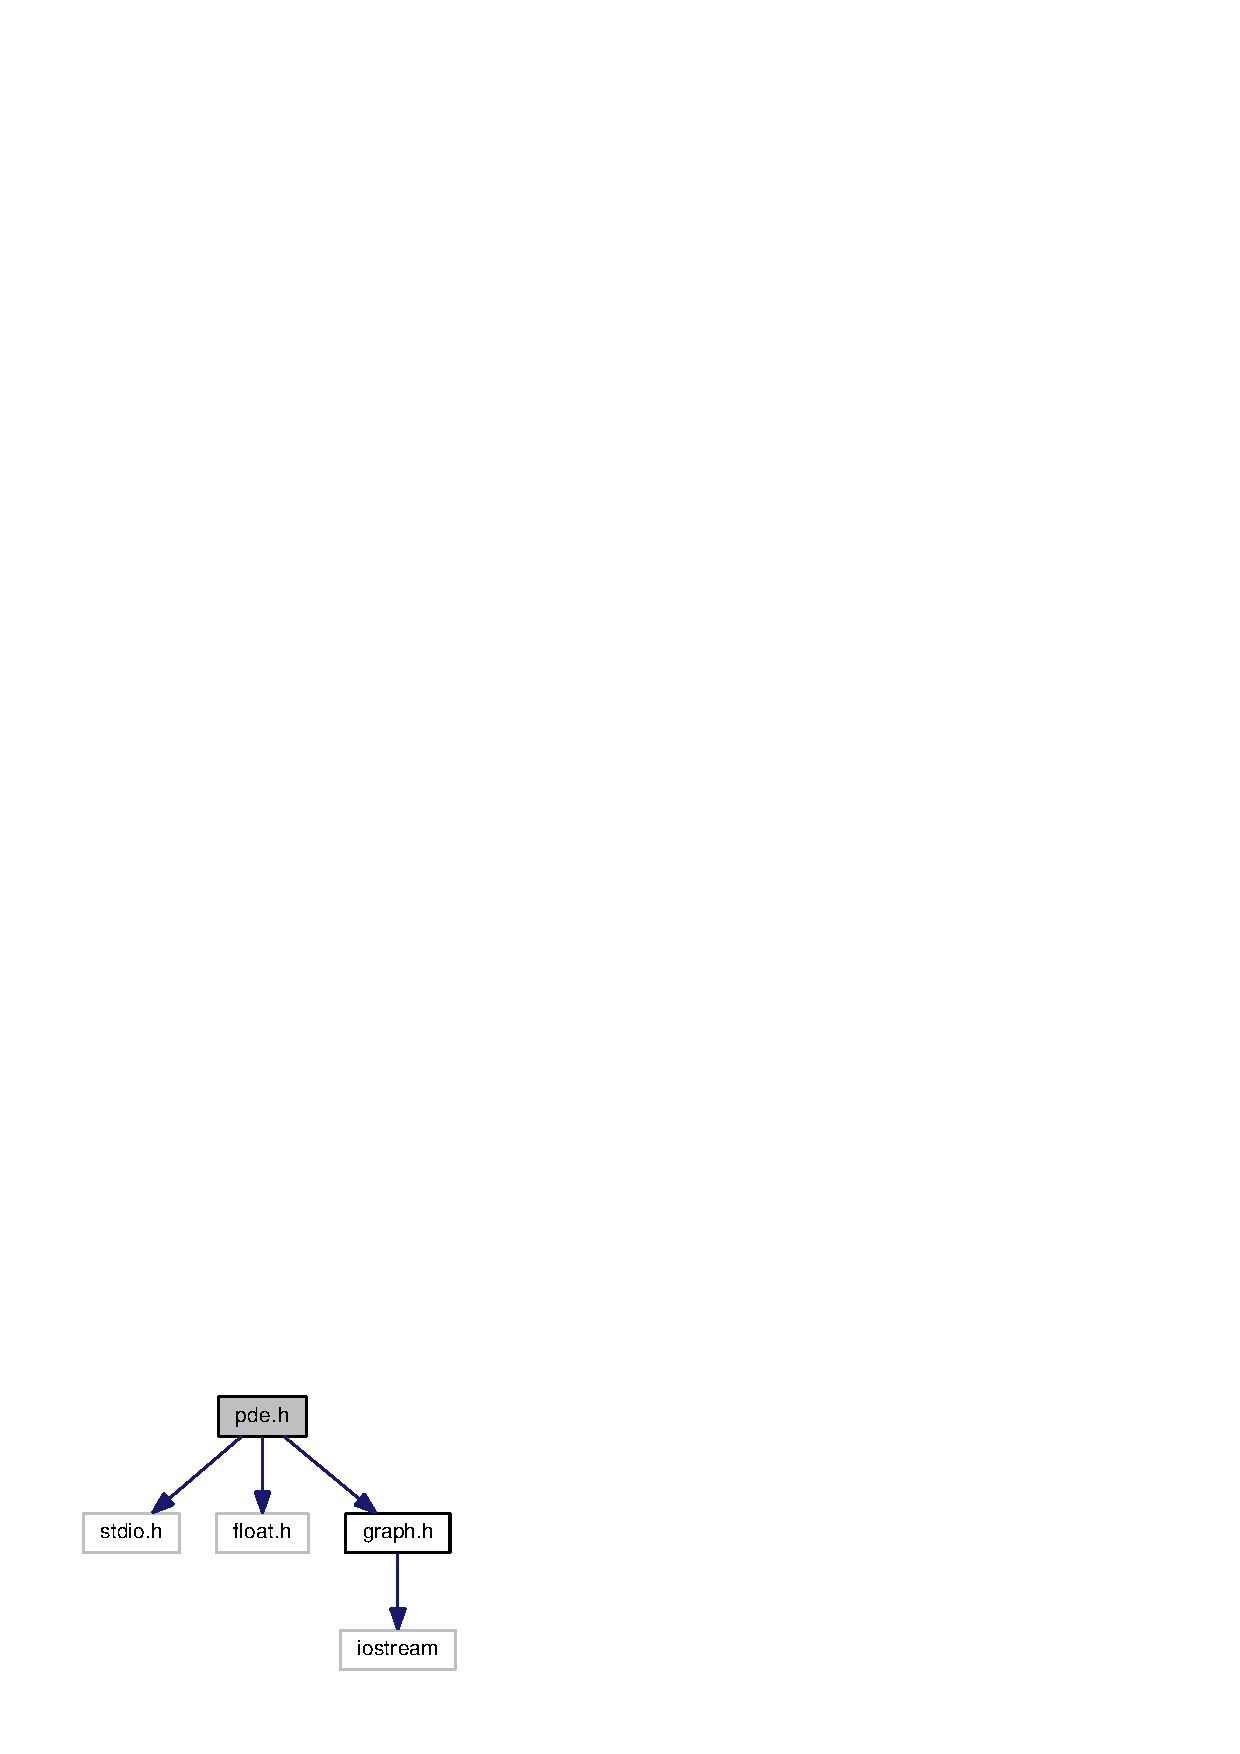
\includegraphics[width=222pt]{pde_8h__incl}
\end{center}
\end{figure}
This graph shows which files directly or indirectly include this file\-:
\nopagebreak
\begin{figure}[H]
\begin{center}
\leavevmode
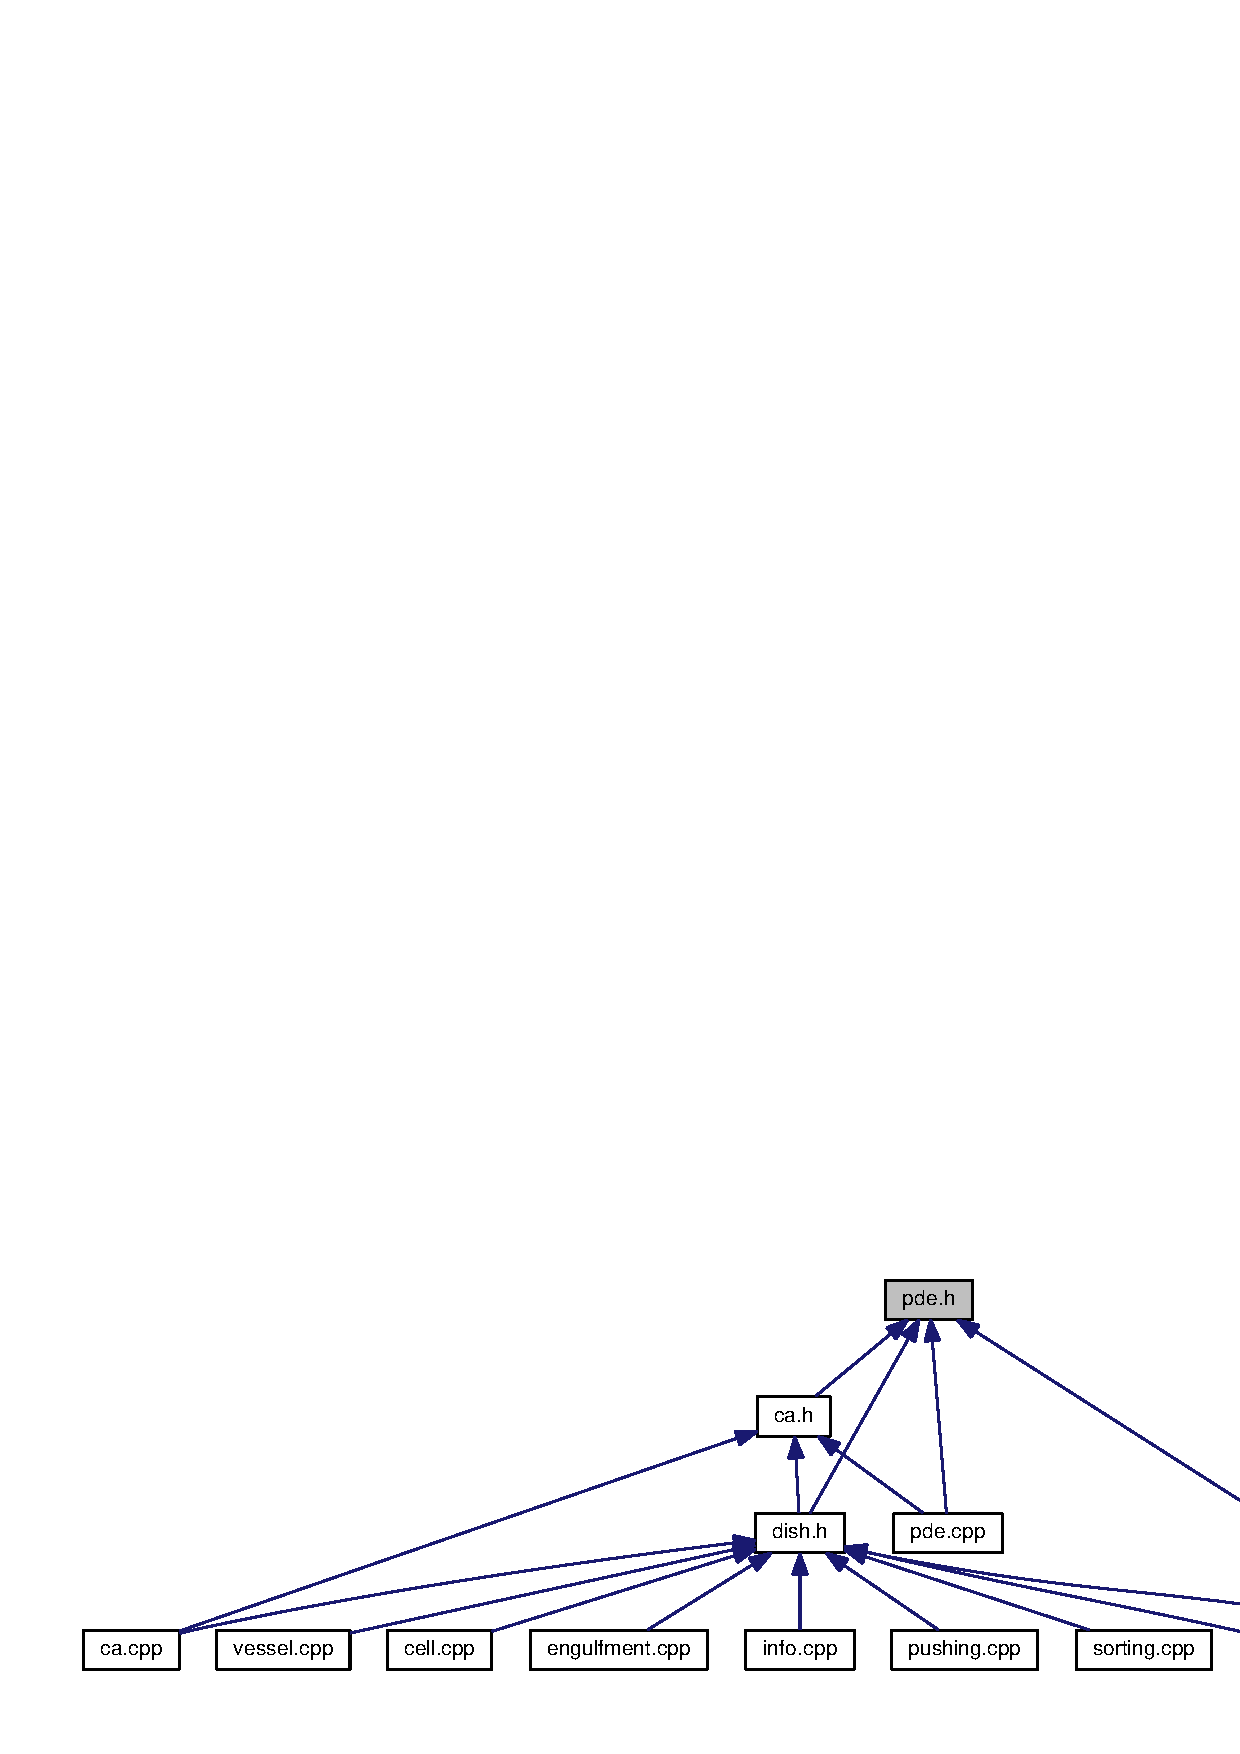
\includegraphics[width=350pt]{pde_8h__dep__incl}
\end{center}
\end{figure}
\subsection*{Classes}
\begin{DoxyCompactItemize}
\item 
class {\bf P\-D\-E}
\end{DoxyCompactItemize}

\section{pushing.\-cpp File Reference}
\label{pushing_8cpp}\index{pushing.\-cpp@{pushing.\-cpp}}
{\ttfamily \#include $<$stdio.\-h$>$}\\*
{\ttfamily \#include $<$malloc.\-h$>$}\\*
{\ttfamily \#include $<$iostream$>$}\\*
{\ttfamily \#include $<$cstdlib$>$}\\*
{\ttfamily \#include $<$algorithm$>$}\\*
{\ttfamily \#include $<$fstream$>$}\\*
{\ttfamily \#include $<$math.\-h$>$}\\*
{\ttfamily \#include \char`\"{}dish.\-h\char`\"{}}\\*
{\ttfamily \#include \char`\"{}random.\-h\char`\"{}}\\*
{\ttfamily \#include \char`\"{}cell.\-h\char`\"{}}\\*
{\ttfamily \#include \char`\"{}info.\-h\char`\"{}}\\*
{\ttfamily \#include \char`\"{}parameter.\-h\char`\"{}}\\*
{\ttfamily \#include \char`\"{}sqr.\-h\char`\"{}}\\*
{\ttfamily \#include \char`\"{}x11graph.\-h\char`\"{}}\\*
Include dependency graph for pushing.\-cpp\-:
\nopagebreak
\begin{figure}[H]
\begin{center}
\leavevmode
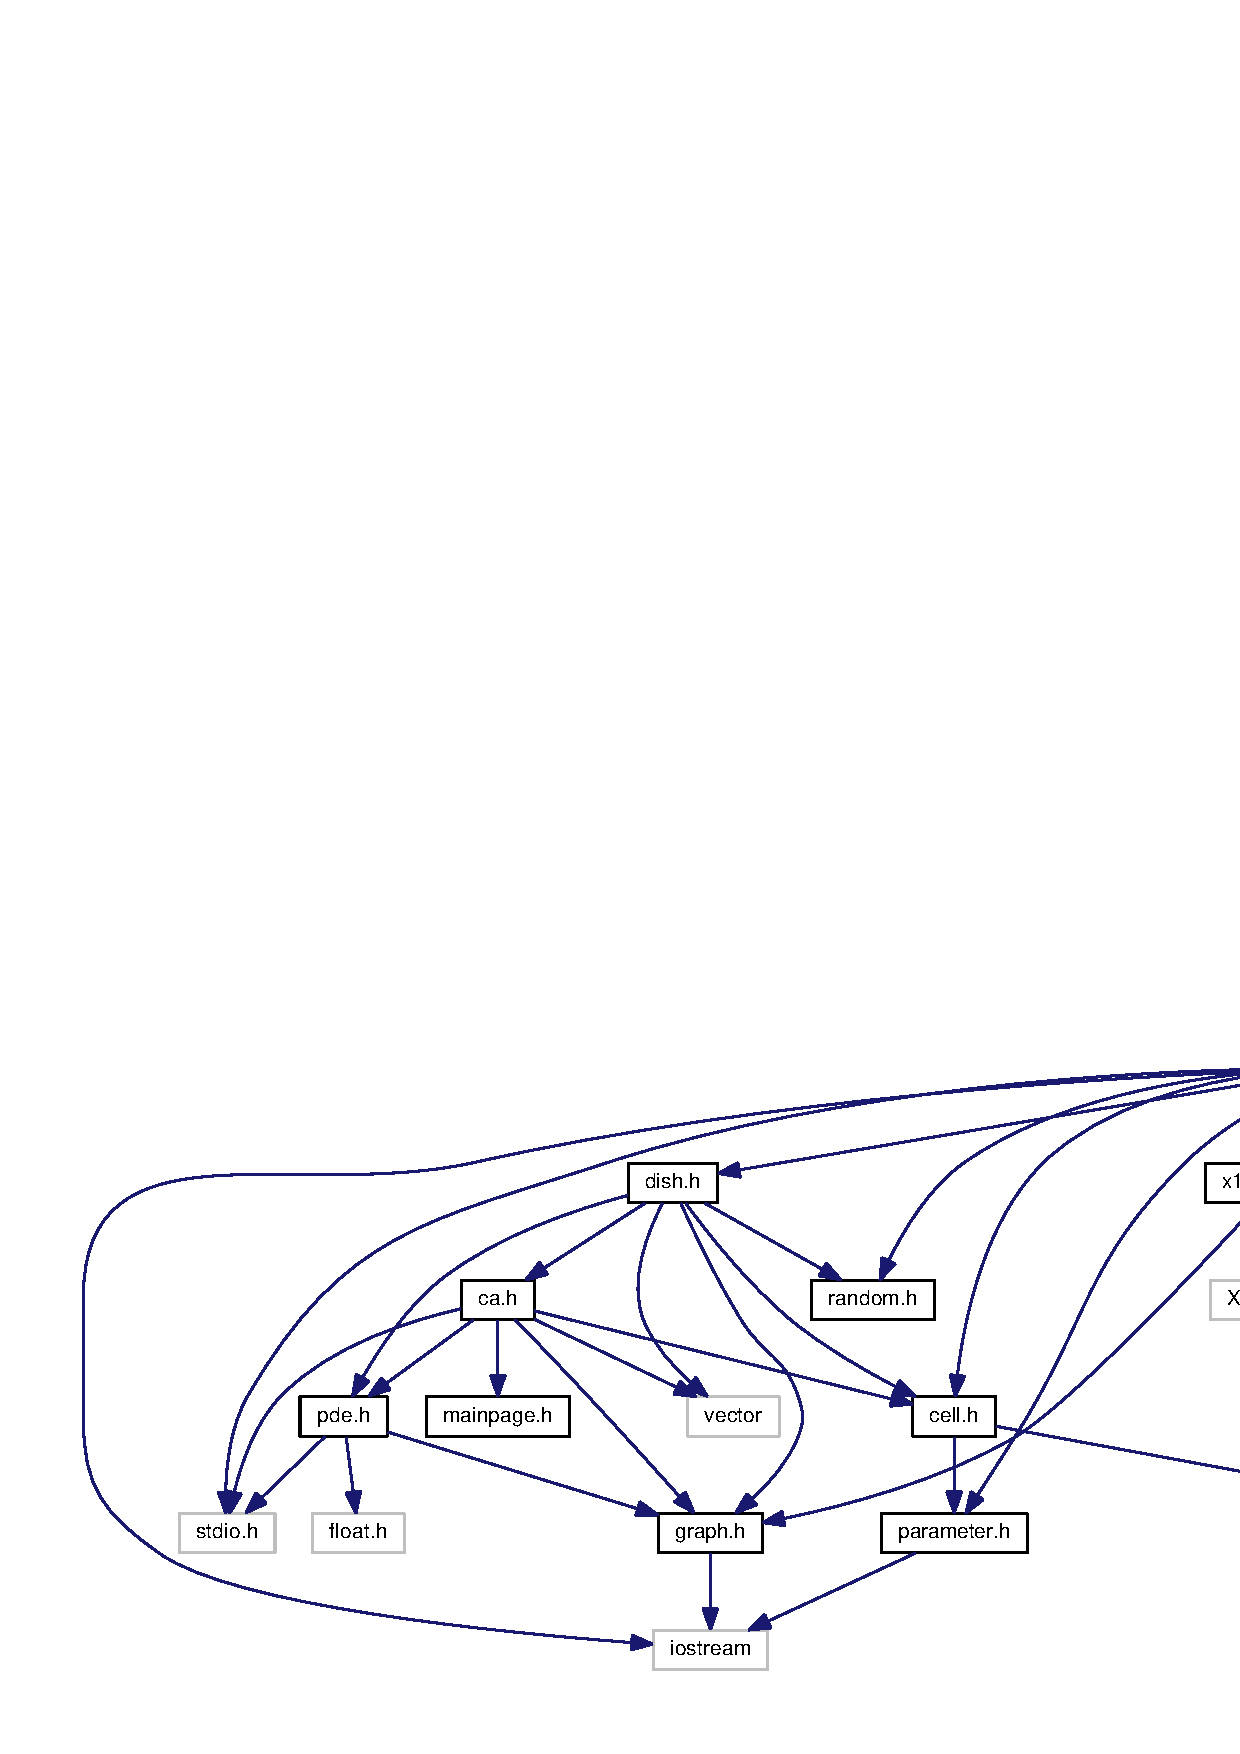
\includegraphics[width=350pt]{pushing_8cpp__incl}
\end{center}
\end{figure}

\section{qt3graph.\-cpp File Reference}
\label{qt3graph_8cpp}\index{qt3graph.\-cpp@{qt3graph.\-cpp}}
{\ttfamily \#include $<$qapplication.\-h$>$}\\*
{\ttfamily \#include $<$qwidget.\-h$>$}\\*
{\ttfamily \#include $<$qlabel.\-h$>$}\\*
{\ttfamily \#include $<$qpainter.\-h$>$}\\*
{\ttfamily \#include $<$qpicture.\-h$>$}\\*
{\ttfamily \#include $<$malloc.\-h$>$}\\*
{\ttfamily \#include $<$iostream$>$}\\*
{\ttfamily \#include $<$qtimer.\-h$>$}\\*
{\ttfamily \#include $<$qpixmap.\-h$>$}\\*
{\ttfamily \#include $<$qimage.\-h$>$}\\*
{\ttfamily \#include $<$qstrlist.\-h$>$}\\*
{\ttfamily \#include \char`\"{}qtgraph.\-h\char`\"{}}\\*
{\ttfamily \#include \char`\"{}parameter.\-h\char`\"{}}\\*
Include dependency graph for qt3graph.\-cpp\-:
\nopagebreak
\begin{figure}[H]
\begin{center}
\leavevmode
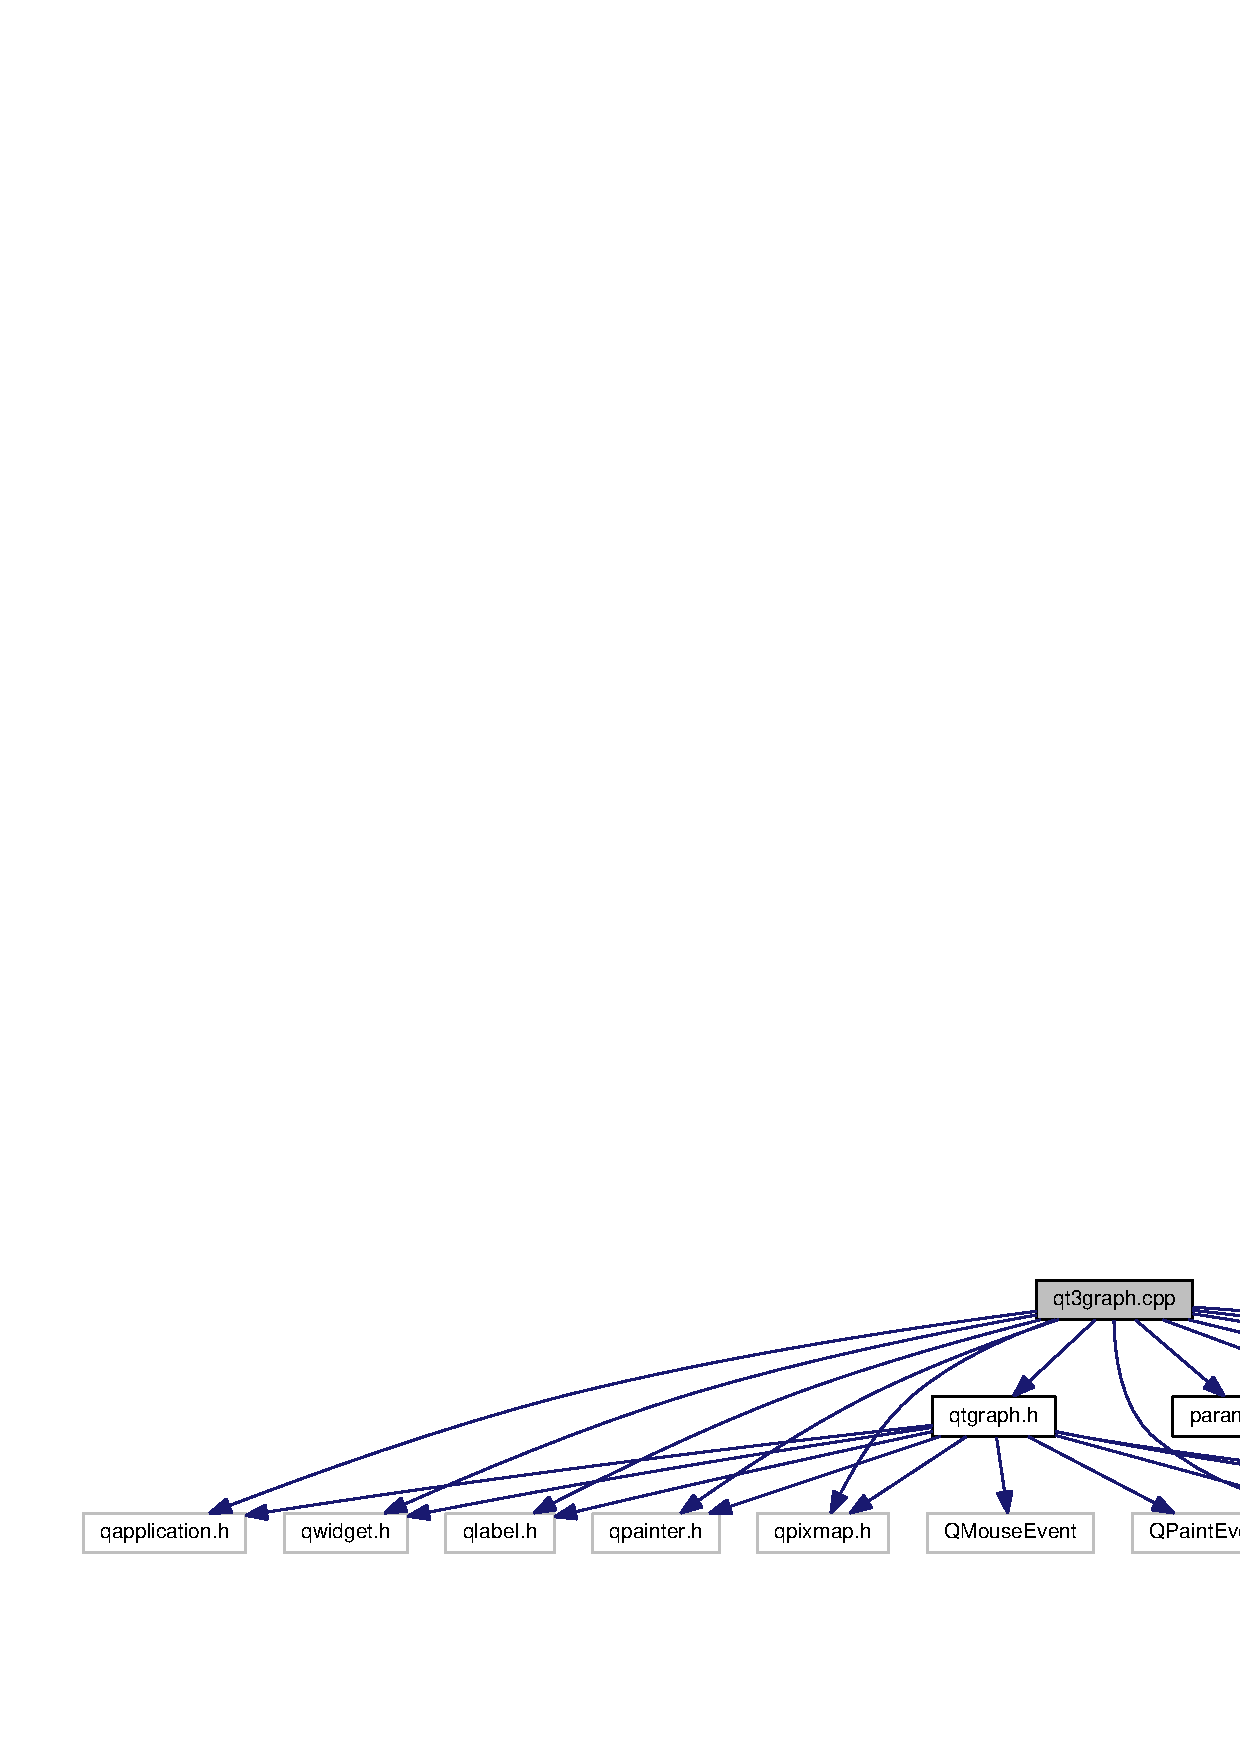
\includegraphics[width=350pt]{qt3graph_8cpp__incl}
\end{center}
\end{figure}

\section{qtgraph.\-cpp File Reference}
\label{qtgraph_8cpp}\index{qtgraph.\-cpp@{qtgraph.\-cpp}}
{\ttfamily \#include $<$qapplication.\-h$>$}\\*
{\ttfamily \#include $<$qwidget.\-h$>$}\\*
{\ttfamily \#include $<$qlabel.\-h$>$}\\*
{\ttfamily \#include $<$qpainter.\-h$>$}\\*
{\ttfamily \#include $<$q3picture.\-h$>$}\\*
{\ttfamily \#include $<$Q\-Palette$>$}\\*
{\ttfamily \#include $<$Q\-Mouse\-Event$>$}\\*
{\ttfamily \#include $<$Q\-Paint\-Event$>$}\\*
{\ttfamily \#include $<$Q\-Image\-Writer$>$}\\*
{\ttfamily \#include $<$malloc.\-h$>$}\\*
{\ttfamily \#include $<$iostream$>$}\\*
{\ttfamily \#include $<$qtimer.\-h$>$}\\*
{\ttfamily \#include $<$qpixmap.\-h$>$}\\*
{\ttfamily \#include $<$qimage.\-h$>$}\\*
{\ttfamily \#include $<$q3strlist.\-h$>$}\\*
{\ttfamily \#include $<$Q\-Resize\-Event$>$}\\*
{\ttfamily \#include \char`\"{}qtgraph.\-h\char`\"{}}\\*
{\ttfamily \#include \char`\"{}parameter.\-h\char`\"{}}\\*
Include dependency graph for qtgraph.\-cpp\-:
\nopagebreak
\begin{figure}[H]
\begin{center}
\leavevmode
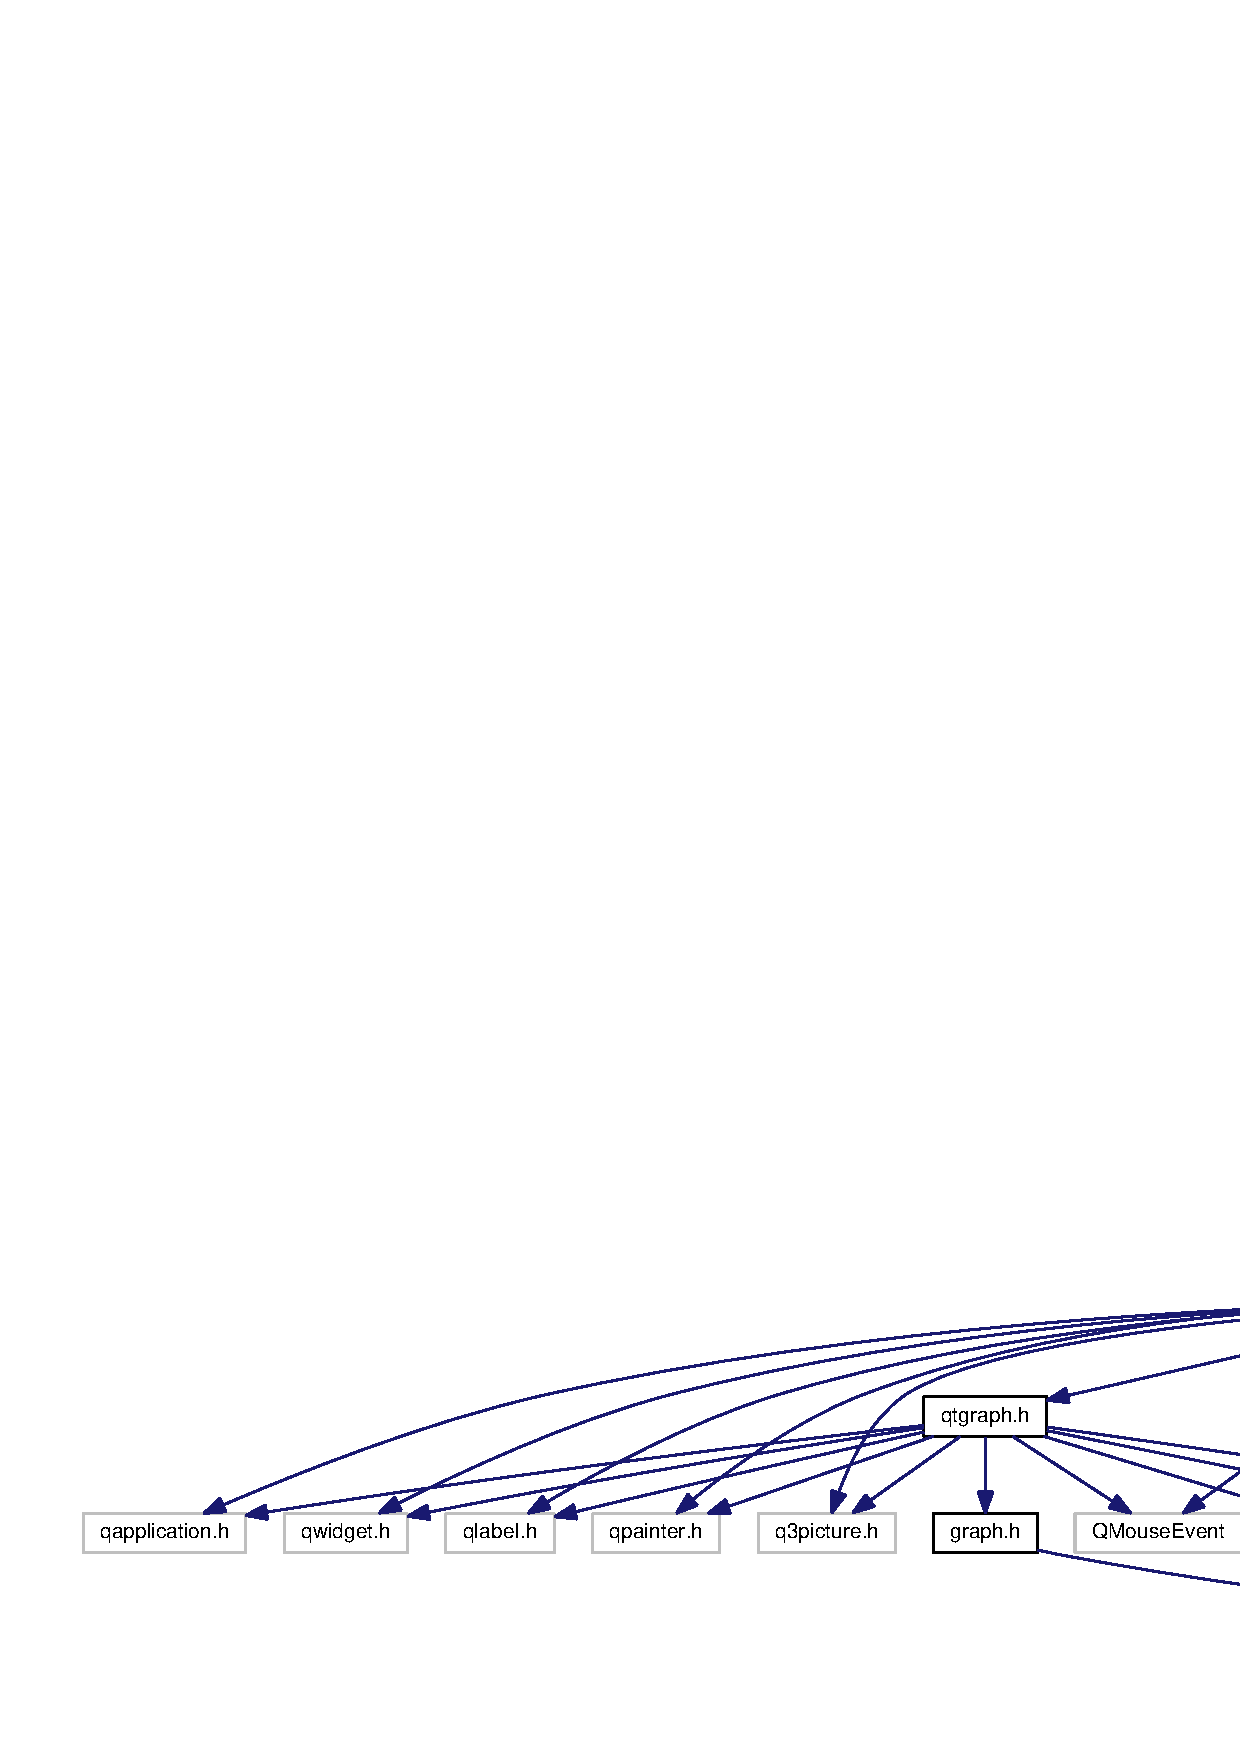
\includegraphics[width=350pt]{qtgraph_8cpp__incl}
\end{center}
\end{figure}

\section{qtgraph.\-h File Reference}
\label{qtgraph_8h}\index{qtgraph.\-h@{qtgraph.\-h}}
{\ttfamily \#include $<$qwidget.\-h$>$}\\*
{\ttfamily \#include $<$qlabel.\-h$>$}\\*
{\ttfamily \#include $<$qpainter.\-h$>$}\\*
{\ttfamily \#include $<$q3picture.\-h$>$}\\*
{\ttfamily \#include $<$qpixmap.\-h$>$}\\*
{\ttfamily \#include $<$Q\-Mouse\-Event$>$}\\*
{\ttfamily \#include $<$Q\-Paint\-Event$>$}\\*
{\ttfamily \#include $<$Q\-Resize\-Event$>$}\\*
{\ttfamily \#include \char`\"{}graph.\-h\char`\"{}}\\*
{\ttfamily \#include $<$qapplication.\-h$>$}\\*
Include dependency graph for qtgraph.\-h\-:
\nopagebreak
\begin{figure}[H]
\begin{center}
\leavevmode
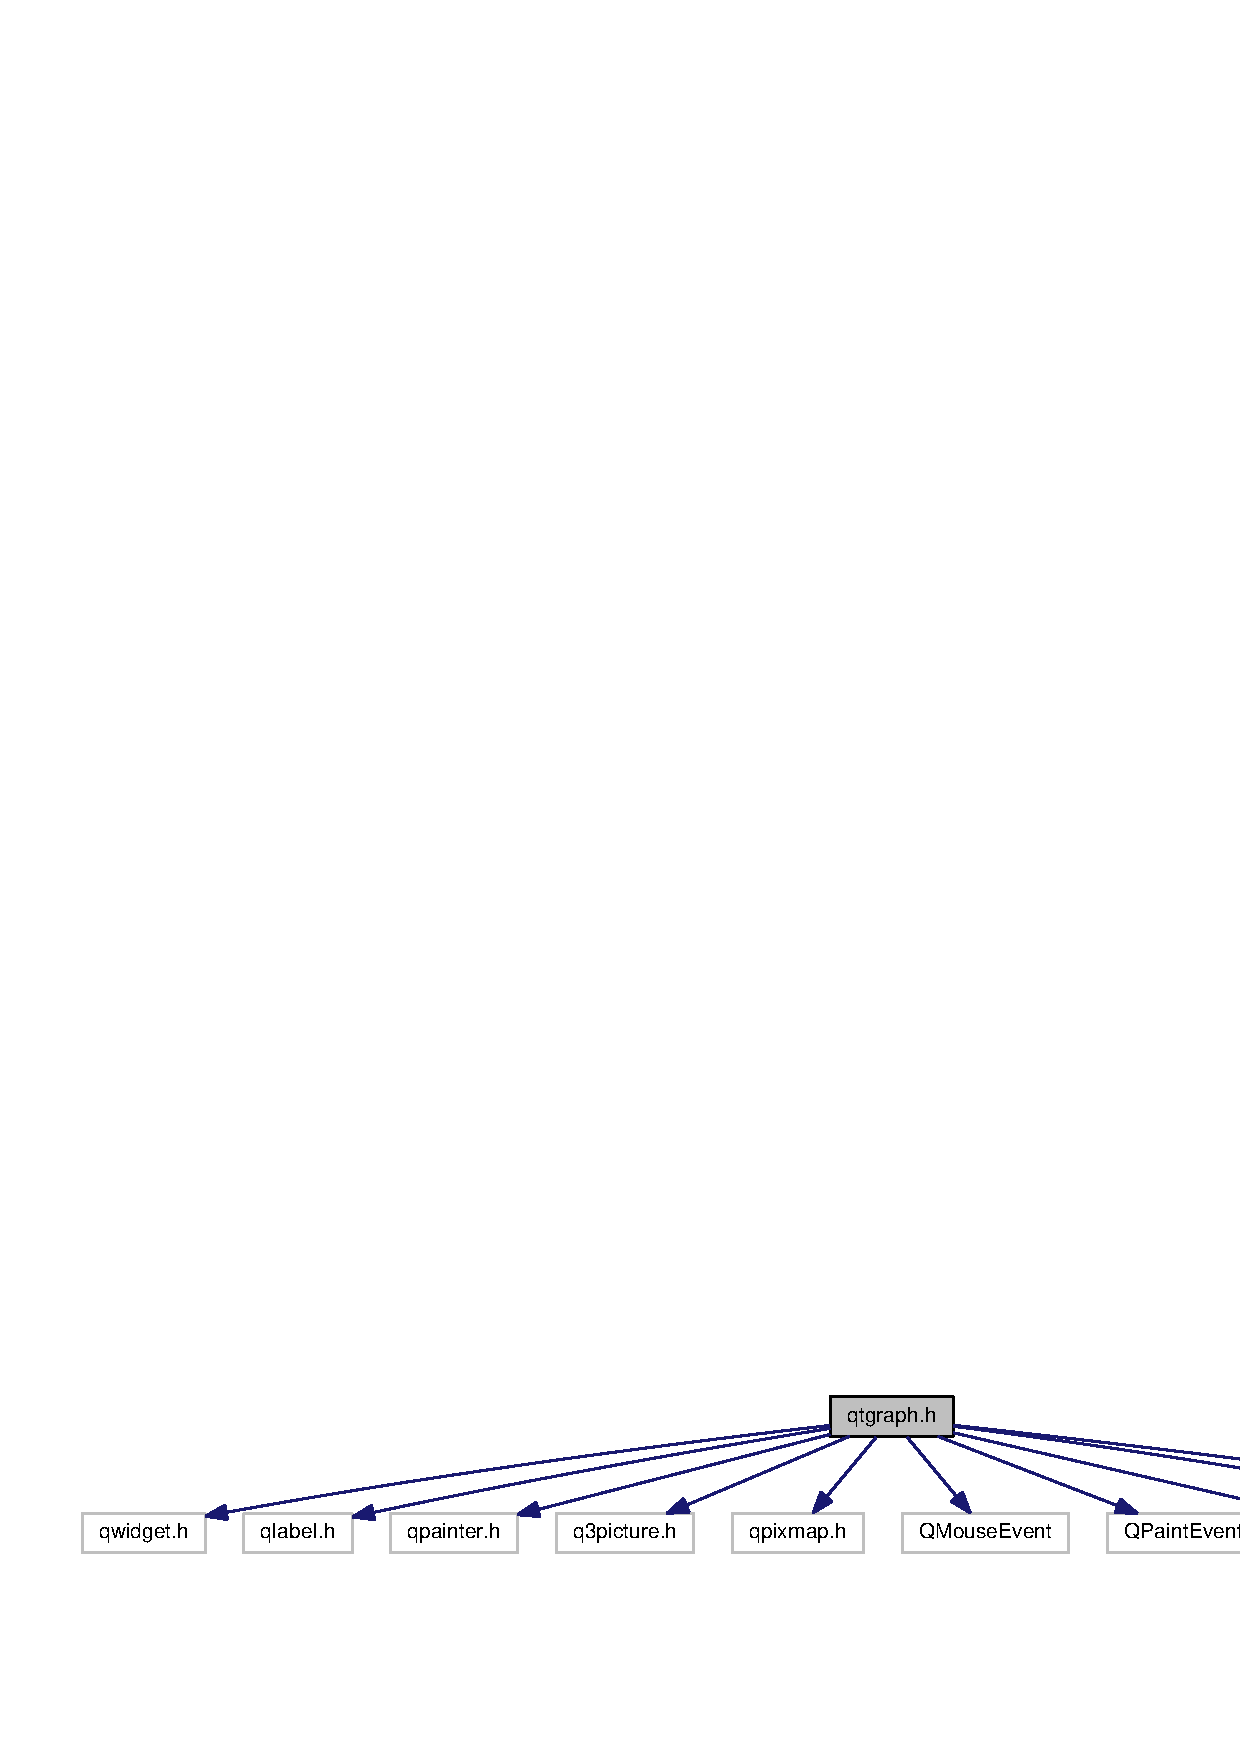
\includegraphics[width=350pt]{qtgraph_8h__incl}
\end{center}
\end{figure}
This graph shows which files directly or indirectly include this file\-:
\nopagebreak
\begin{figure}[H]
\begin{center}
\leavevmode
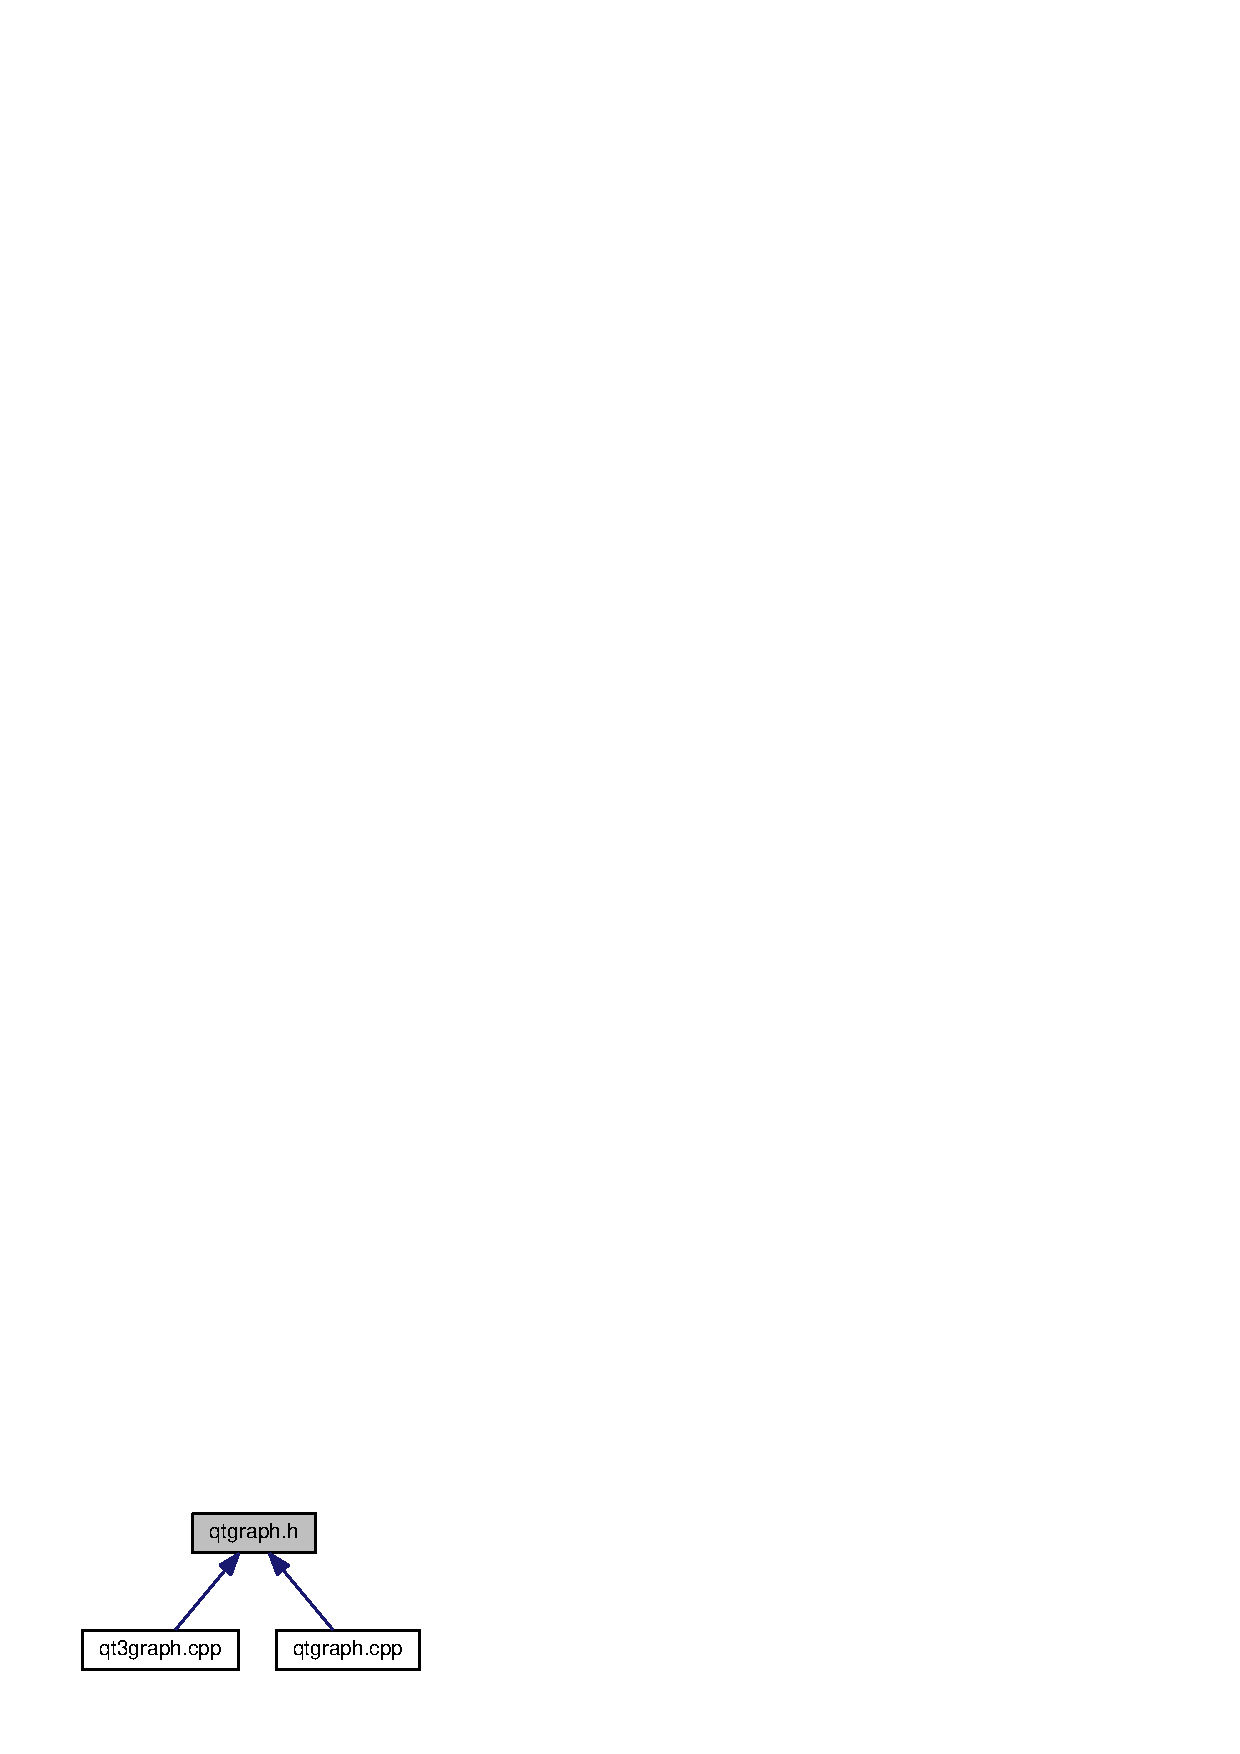
\includegraphics[width=205pt]{qtgraph_8h__dep__incl}
\end{center}
\end{figure}
\subsection*{Classes}
\begin{DoxyCompactItemize}
\item 
class {\bf Qt\-Graphics}
\end{DoxyCompactItemize}
\subsection*{Macros}
\begin{DoxyCompactItemize}
\item 
\#define {\bf T\-I\-M\-E\-S\-T\-E\-P}~void {\bf Qt\-Graphics\-::\-Time\-Step}(void)
\end{DoxyCompactItemize}


\subsection{Macro Definition Documentation}
\index{qtgraph.\-h@{qtgraph.\-h}!T\-I\-M\-E\-S\-T\-E\-P@{T\-I\-M\-E\-S\-T\-E\-P}}
\index{T\-I\-M\-E\-S\-T\-E\-P@{T\-I\-M\-E\-S\-T\-E\-P}!qtgraph.h@{qtgraph.\-h}}
\subsubsection[{T\-I\-M\-E\-S\-T\-E\-P}]{\setlength{\rightskip}{0pt plus 5cm}\#define T\-I\-M\-E\-S\-T\-E\-P~void {\bf Qt\-Graphics\-::\-Time\-Step}(void)}\label{qtgraph_8h_a68ee019dafc12ee47d427cda7f17713e}

\section{random.\-cpp File Reference}
\label{random_8cpp}\index{random.\-cpp@{random.\-cpp}}
{\ttfamily \#include $<$stdio.\-h$>$}\\*
{\ttfamily \#include $<$stdlib.\-h$>$}\\*
{\ttfamily \#include $<$sys/timeb.\-h$>$}\\*
{\ttfamily \#include $<$iostream$>$}\\*
{\ttfamily \#include \char`\"{}random.\-h\char`\"{}}\\*
Include dependency graph for random.\-cpp\-:
\nopagebreak
\begin{figure}[H]
\begin{center}
\leavevmode
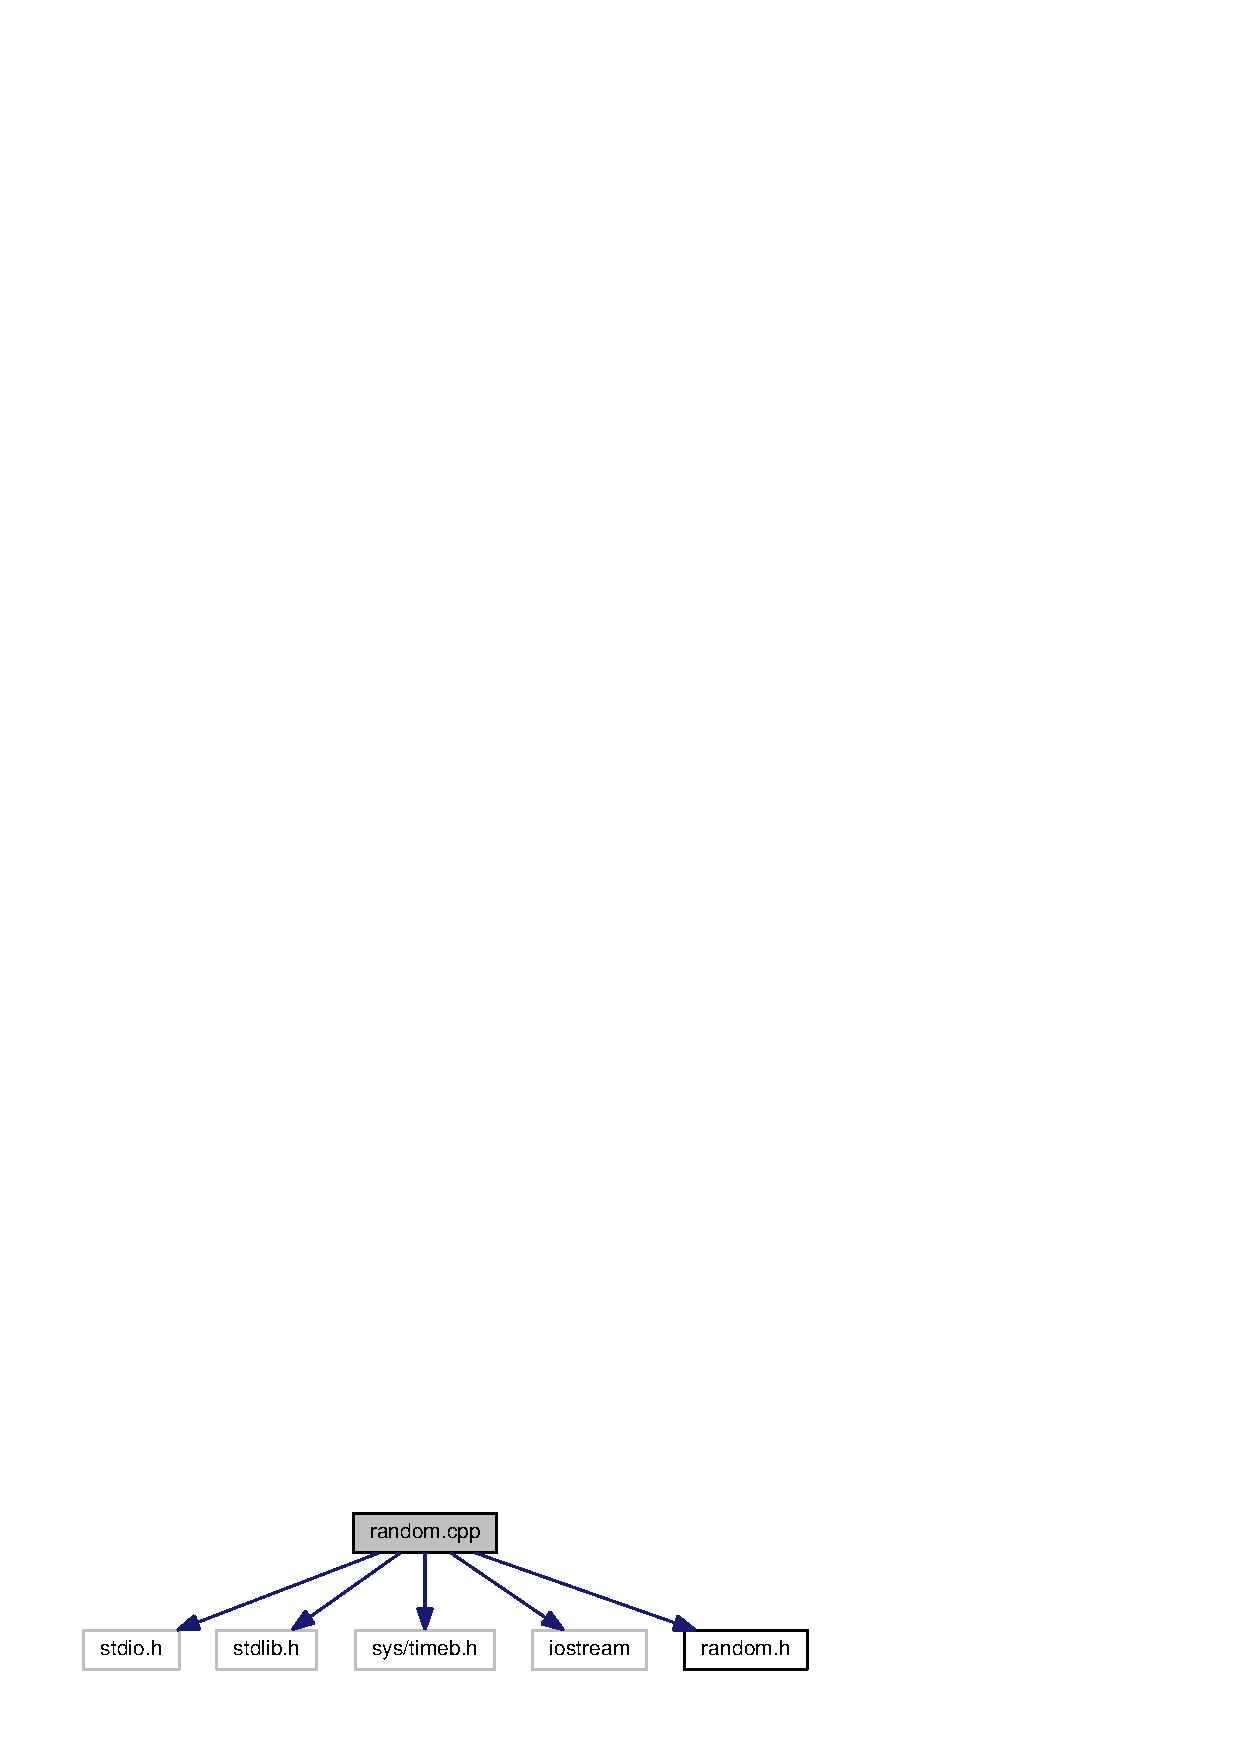
\includegraphics[width=350pt]{random_8cpp__incl}
\end{center}
\end{figure}
\subsection*{Functions}
\begin{DoxyCompactItemize}
\item 
double {\bf R\-A\-N\-D\-O\-M} (void)
\item 
int {\bf Seed} (int seed)
\item 
long {\bf Random\-Number} (long {\bf max})
\item 
void {\bf Ask\-Seed} (void)
\item 
int {\bf Randomize} (void)
\end{DoxyCompactItemize}


\subsection{Function Documentation}
\index{random.\-cpp@{random.\-cpp}!Ask\-Seed@{Ask\-Seed}}
\index{Ask\-Seed@{Ask\-Seed}!random.cpp@{random.\-cpp}}
\subsubsection[{Ask\-Seed}]{\setlength{\rightskip}{0pt plus 5cm}void Ask\-Seed (
\begin{DoxyParamCaption}
\item[{void}]{}
\end{DoxyParamCaption}
)}\label{random_8cpp_ac5f0897c1e7606a95cb1cce33cc44194}
Interactively ask for the seed 
\begin{DoxyParams}{Parameters}
{\em void} & \\
\hline
\end{DoxyParams}
\begin{DoxyReturn}{Returns}
void 
\end{DoxyReturn}


References Seed().

\index{random.\-cpp@{random.\-cpp}!R\-A\-N\-D\-O\-M@{R\-A\-N\-D\-O\-M}}
\index{R\-A\-N\-D\-O\-M@{R\-A\-N\-D\-O\-M}!random.cpp@{random.\-cpp}}
\subsubsection[{R\-A\-N\-D\-O\-M}]{\setlength{\rightskip}{0pt plus 5cm}double R\-A\-N\-D\-O\-M (
\begin{DoxyParamCaption}
\item[{void}]{}
\end{DoxyParamCaption}
)}\label{random_8cpp_a116ead99728070ce429280e9c976ff7f}
\begin{DoxyReturn}{Returns}
A random double between 0 and 1 
\end{DoxyReturn}


References F\-A\-C, M\-B\-I\-G, M\-S\-E\-E\-D, and M\-Z.



Referenced by Cellular\-Potts\-::\-Amoebae\-Move(), Cellular\-Potts\-::\-Grow\-In\-Cells(), Random\-Number(), and Seed().

\index{random.\-cpp@{random.\-cpp}!Randomize@{Randomize}}
\index{Randomize@{Randomize}!random.cpp@{random.\-cpp}}
\subsubsection[{Randomize}]{\setlength{\rightskip}{0pt plus 5cm}int Randomize (
\begin{DoxyParamCaption}
\item[{void}]{}
\end{DoxyParamCaption}
)}\label{random_8cpp_ae21c32bc12a35221312b6ba099cfbfc3}
Make a random seed based on the local time 
\begin{DoxyParams}{Parameters}
{\em void} & \\
\hline
\end{DoxyParams}
\begin{DoxyReturn}{Returns}
void 
\end{DoxyReturn}


References Seed().



Referenced by Seed().

\index{random.\-cpp@{random.\-cpp}!Random\-Number@{Random\-Number}}
\index{Random\-Number@{Random\-Number}!random.cpp@{random.\-cpp}}
\subsubsection[{Random\-Number}]{\setlength{\rightskip}{0pt plus 5cm}long Random\-Number (
\begin{DoxyParamCaption}
\item[{long}]{max}
\end{DoxyParamCaption}
)}\label{random_8cpp_ab49f60b2bb33d03c1371c7a3fa46b1a6}
Returns a random integer value between 1 and 'max' 
\begin{DoxyParams}{Parameters}
{\em The} & maximum value (long) \\
\hline
\end{DoxyParams}
\begin{DoxyReturn}{Returns}
A random integer (long) 
\end{DoxyReturn}


References R\-A\-N\-D\-O\-M().



Referenced by Cellular\-Potts\-::\-Grow\-In\-Cells(), Cellular\-Potts\-::\-Set\-Random\-Types(), and Cellular\-Potts\-::\-Throw\-In\-Cells().

\index{random.\-cpp@{random.\-cpp}!Seed@{Seed}}
\index{Seed@{Seed}!random.cpp@{random.\-cpp}}
\subsubsection[{Seed}]{\setlength{\rightskip}{0pt plus 5cm}int Seed (
\begin{DoxyParamCaption}
\item[{int}]{seed}
\end{DoxyParamCaption}
)}\label{random_8cpp_a12de90ae172738036dbb252c0e72dc66}

\begin{DoxyParams}{Parameters}
{\em An} & integer random seed \\
\hline
\end{DoxyParams}
\begin{DoxyReturn}{Returns}
the random seed 
\end{DoxyReturn}


References R\-A\-N\-D\-O\-M(), and Randomize().



Referenced by Ask\-Seed(), and Randomize().


\section{random.\-h File Reference}
\label{random_8h}\index{random.\-h@{random.\-h}}
This graph shows which files directly or indirectly include this file\-:
\nopagebreak
\begin{figure}[H]
\begin{center}
\leavevmode
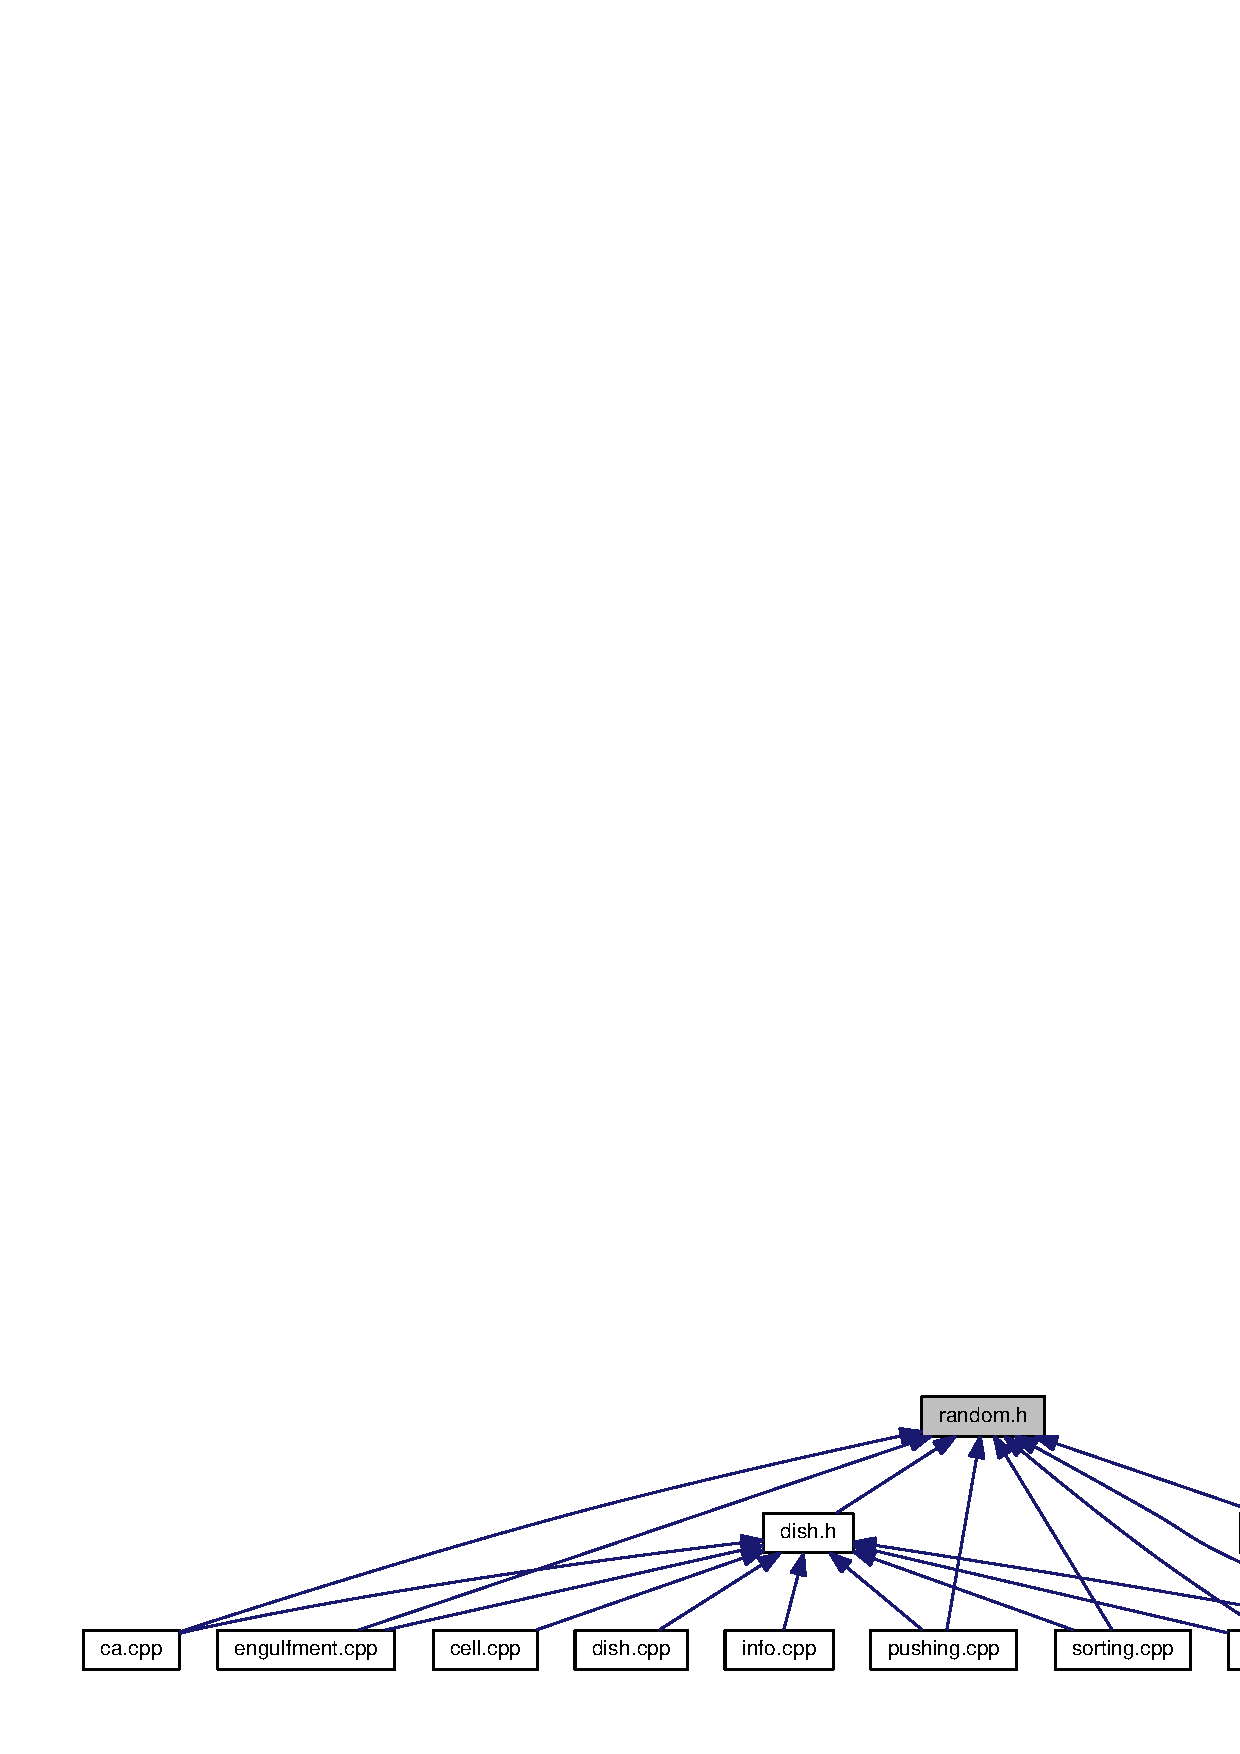
\includegraphics[width=350pt]{random_8h__dep__incl}
\end{center}
\end{figure}
\subsection*{Macros}
\begin{DoxyCompactItemize}
\item 
\#define {\bf M\-B\-I\-G}~1000000000
\item 
\#define {\bf M\-S\-E\-E\-D}~161803398
\item 
\#define {\bf M\-Z}~0
\item 
\#define {\bf F\-A\-C}~(1.\-0/{\bf M\-B\-I\-G})
\end{DoxyCompactItemize}
\subsection*{Functions}
\begin{DoxyCompactItemize}
\item 
double {\bf R\-A\-N\-D\-O\-M} ()
\item 
int {\bf Seed} (int seed)
\item 
long {\bf Random\-Number} (long {\bf max})
\item 
void {\bf Ask\-Seed} ()
\item 
int {\bf Randomize} (void)
\end{DoxyCompactItemize}


\subsection{Macro Definition Documentation}
\index{random.\-h@{random.\-h}!F\-A\-C@{F\-A\-C}}
\index{F\-A\-C@{F\-A\-C}!random.h@{random.\-h}}
\subsubsection[{F\-A\-C}]{\setlength{\rightskip}{0pt plus 5cm}\#define F\-A\-C~(1.\-0/{\bf M\-B\-I\-G})}\label{random_8h_a8c3c7226e23b36189d1ec6b7d3504499}


Referenced by R\-A\-N\-D\-O\-M().

\index{random.\-h@{random.\-h}!M\-B\-I\-G@{M\-B\-I\-G}}
\index{M\-B\-I\-G@{M\-B\-I\-G}!random.h@{random.\-h}}
\subsubsection[{M\-B\-I\-G}]{\setlength{\rightskip}{0pt plus 5cm}\#define M\-B\-I\-G~1000000000}\label{random_8h_a31be5e3096afa10fc67bd629dd9332e7}


Referenced by R\-A\-N\-D\-O\-M().

\index{random.\-h@{random.\-h}!M\-S\-E\-E\-D@{M\-S\-E\-E\-D}}
\index{M\-S\-E\-E\-D@{M\-S\-E\-E\-D}!random.h@{random.\-h}}
\subsubsection[{M\-S\-E\-E\-D}]{\setlength{\rightskip}{0pt plus 5cm}\#define M\-S\-E\-E\-D~161803398}\label{random_8h_aa0e8039431bb68581133ef4c1dbbe71d}


Referenced by R\-A\-N\-D\-O\-M().

\index{random.\-h@{random.\-h}!M\-Z@{M\-Z}}
\index{M\-Z@{M\-Z}!random.h@{random.\-h}}
\subsubsection[{M\-Z}]{\setlength{\rightskip}{0pt plus 5cm}\#define M\-Z~0}\label{random_8h_a8dbc2223b1260b0fb5ab3d57bec0f74d}


Referenced by R\-A\-N\-D\-O\-M().



\subsection{Function Documentation}
\index{random.\-h@{random.\-h}!Ask\-Seed@{Ask\-Seed}}
\index{Ask\-Seed@{Ask\-Seed}!random.h@{random.\-h}}
\subsubsection[{Ask\-Seed}]{\setlength{\rightskip}{0pt plus 5cm}void Ask\-Seed (
\begin{DoxyParamCaption}
\item[{void}]{}
\end{DoxyParamCaption}
)}\label{random_8h_a34f7b93b23be476f43d1b1169cbab3c0}
Interactively ask for the seed 
\begin{DoxyParams}{Parameters}
{\em void} & \\
\hline
\end{DoxyParams}
\begin{DoxyReturn}{Returns}
void 
\end{DoxyReturn}


References Seed().

\index{random.\-h@{random.\-h}!R\-A\-N\-D\-O\-M@{R\-A\-N\-D\-O\-M}}
\index{R\-A\-N\-D\-O\-M@{R\-A\-N\-D\-O\-M}!random.h@{random.\-h}}
\subsubsection[{R\-A\-N\-D\-O\-M}]{\setlength{\rightskip}{0pt plus 5cm}double R\-A\-N\-D\-O\-M (
\begin{DoxyParamCaption}
\item[{void}]{}
\end{DoxyParamCaption}
)}\label{random_8h_af26e98955ff2eaaa6f4ee6b09ca07342}
\begin{DoxyReturn}{Returns}
A random double between 0 and 1 
\end{DoxyReturn}
\index{random.\-h@{random.\-h}!Randomize@{Randomize}}
\index{Randomize@{Randomize}!random.h@{random.\-h}}
\subsubsection[{Randomize}]{\setlength{\rightskip}{0pt plus 5cm}int Randomize (
\begin{DoxyParamCaption}
\item[{void}]{}
\end{DoxyParamCaption}
)}\label{random_8h_ae21c32bc12a35221312b6ba099cfbfc3}
Make a random seed based on the local time 
\begin{DoxyParams}{Parameters}
{\em void} & \\
\hline
\end{DoxyParams}
\begin{DoxyReturn}{Returns}
void 
\end{DoxyReturn}


References Seed().



Referenced by Seed().

\index{random.\-h@{random.\-h}!Random\-Number@{Random\-Number}}
\index{Random\-Number@{Random\-Number}!random.h@{random.\-h}}
\subsubsection[{Random\-Number}]{\setlength{\rightskip}{0pt plus 5cm}long Random\-Number (
\begin{DoxyParamCaption}
\item[{long}]{max}
\end{DoxyParamCaption}
)}\label{random_8h_ab49f60b2bb33d03c1371c7a3fa46b1a6}
Returns a random integer value between 1 and 'max' 
\begin{DoxyParams}{Parameters}
{\em The} & maximum value (long) \\
\hline
\end{DoxyParams}
\begin{DoxyReturn}{Returns}
A random integer (long) 
\end{DoxyReturn}


References R\-A\-N\-D\-O\-M().



Referenced by Cellular\-Potts\-::\-Grow\-In\-Cells(), Cellular\-Potts\-::\-Set\-Random\-Types(), and Cellular\-Potts\-::\-Throw\-In\-Cells().

\index{random.\-h@{random.\-h}!Seed@{Seed}}
\index{Seed@{Seed}!random.h@{random.\-h}}
\subsubsection[{Seed}]{\setlength{\rightskip}{0pt plus 5cm}int Seed (
\begin{DoxyParamCaption}
\item[{int}]{seed}
\end{DoxyParamCaption}
)}\label{random_8h_a12de90ae172738036dbb252c0e72dc66}

\begin{DoxyParams}{Parameters}
{\em An} & integer random seed \\
\hline
\end{DoxyParams}
\begin{DoxyReturn}{Returns}
the random seed 
\end{DoxyReturn}


References R\-A\-N\-D\-O\-M(), and Randomize().



Referenced by Ask\-Seed(), and Randomize().


\section{sorting.\-cpp File Reference}
\label{sorting_8cpp}\index{sorting.\-cpp@{sorting.\-cpp}}
{\ttfamily \#include $<$stdio.\-h$>$}\\*
{\ttfamily \#include $<$malloc.\-h$>$}\\*
{\ttfamily \#include $<$iostream$>$}\\*
{\ttfamily \#include $<$cstdlib$>$}\\*
{\ttfamily \#include $<$algorithm$>$}\\*
{\ttfamily \#include $<$fstream$>$}\\*
{\ttfamily \#include $<$math.\-h$>$}\\*
{\ttfamily \#include \char`\"{}dish.\-h\char`\"{}}\\*
{\ttfamily \#include \char`\"{}random.\-h\char`\"{}}\\*
{\ttfamily \#include \char`\"{}cell.\-h\char`\"{}}\\*
{\ttfamily \#include \char`\"{}info.\-h\char`\"{}}\\*
{\ttfamily \#include \char`\"{}parameter.\-h\char`\"{}}\\*
{\ttfamily \#include \char`\"{}sqr.\-h\char`\"{}}\\*
{\ttfamily \#include \char`\"{}x11graph.\-h\char`\"{}}\\*
Include dependency graph for sorting.\-cpp\-:
\nopagebreak
\begin{figure}[H]
\begin{center}
\leavevmode
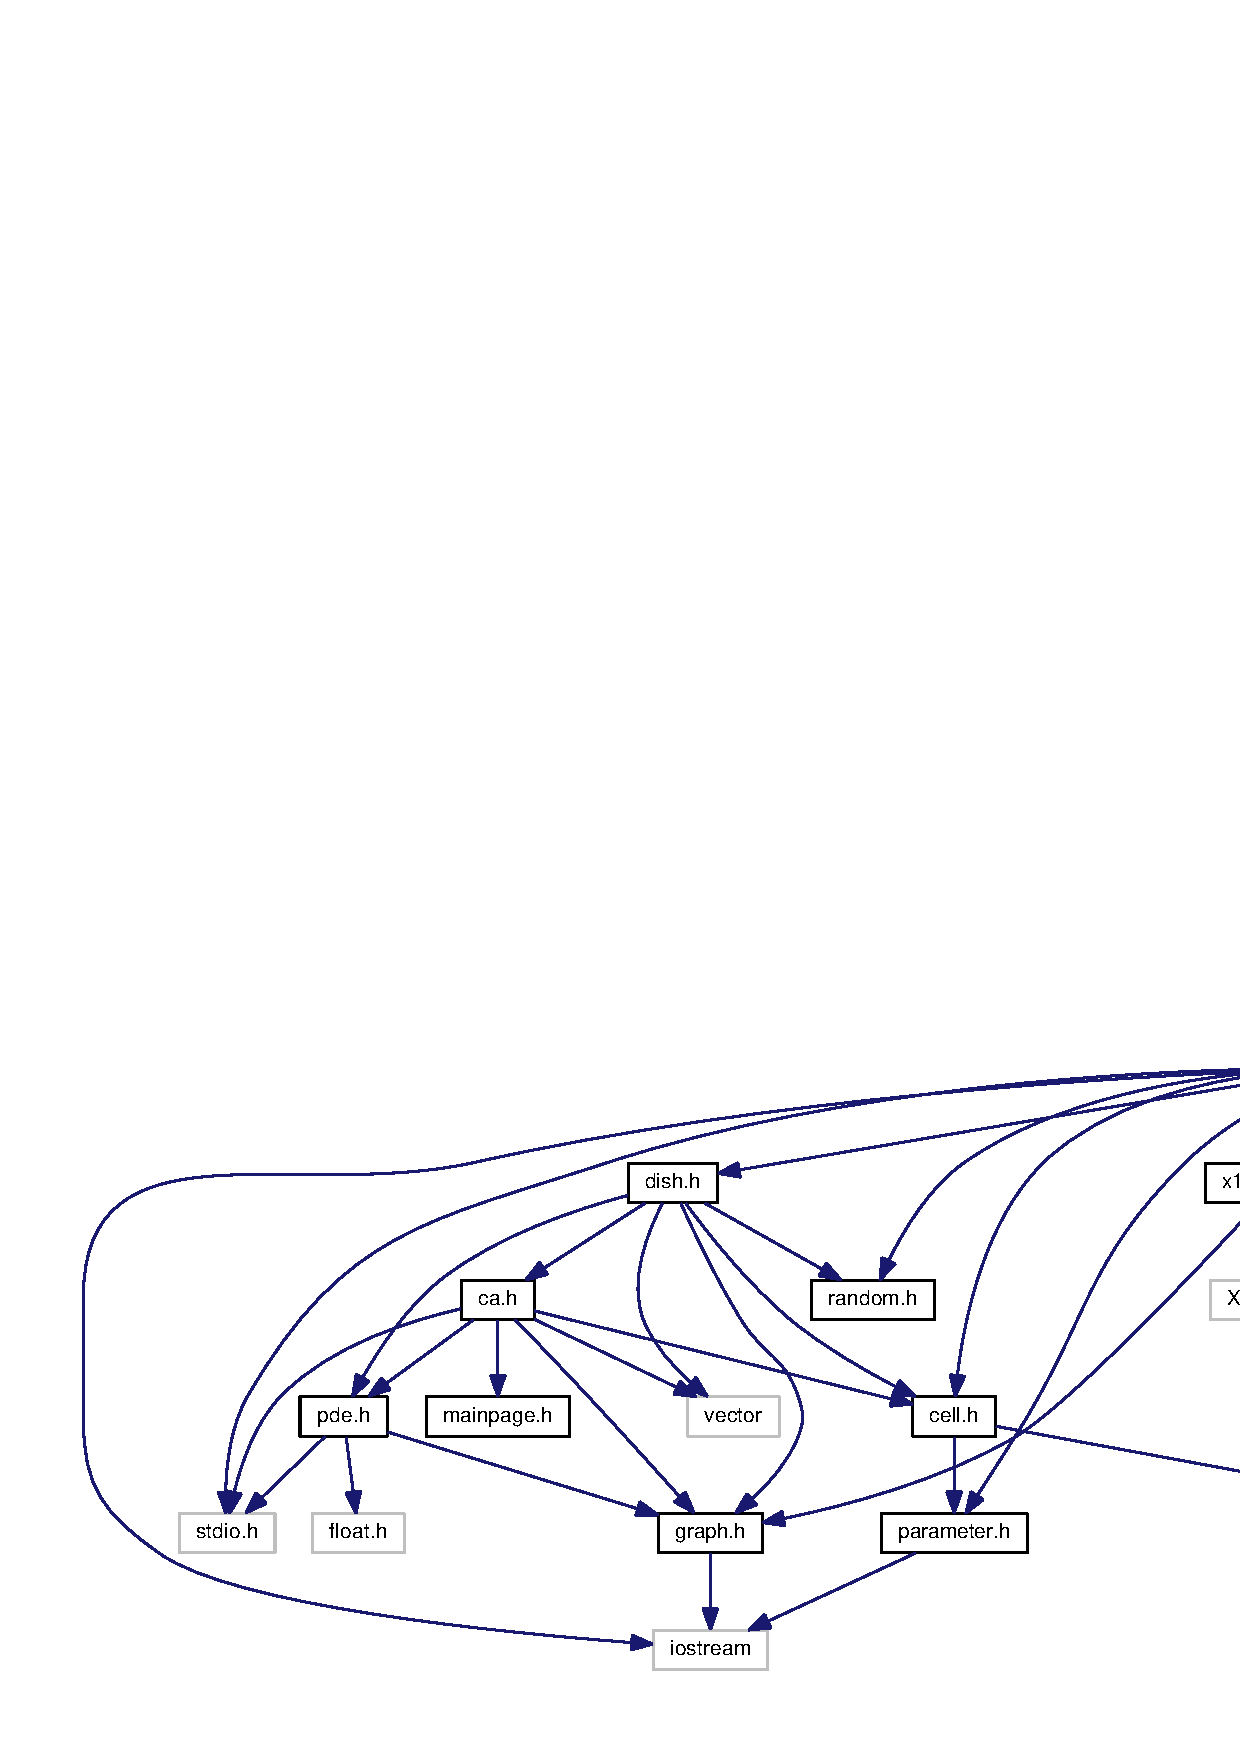
\includegraphics[width=350pt]{sorting_8cpp__incl}
\end{center}
\end{figure}

\section{sqr.\-h File Reference}
\label{sqr_8h}\index{sqr.\-h@{sqr.\-h}}
This graph shows which files directly or indirectly include this file\-:
\nopagebreak
\begin{figure}[H]
\begin{center}
\leavevmode
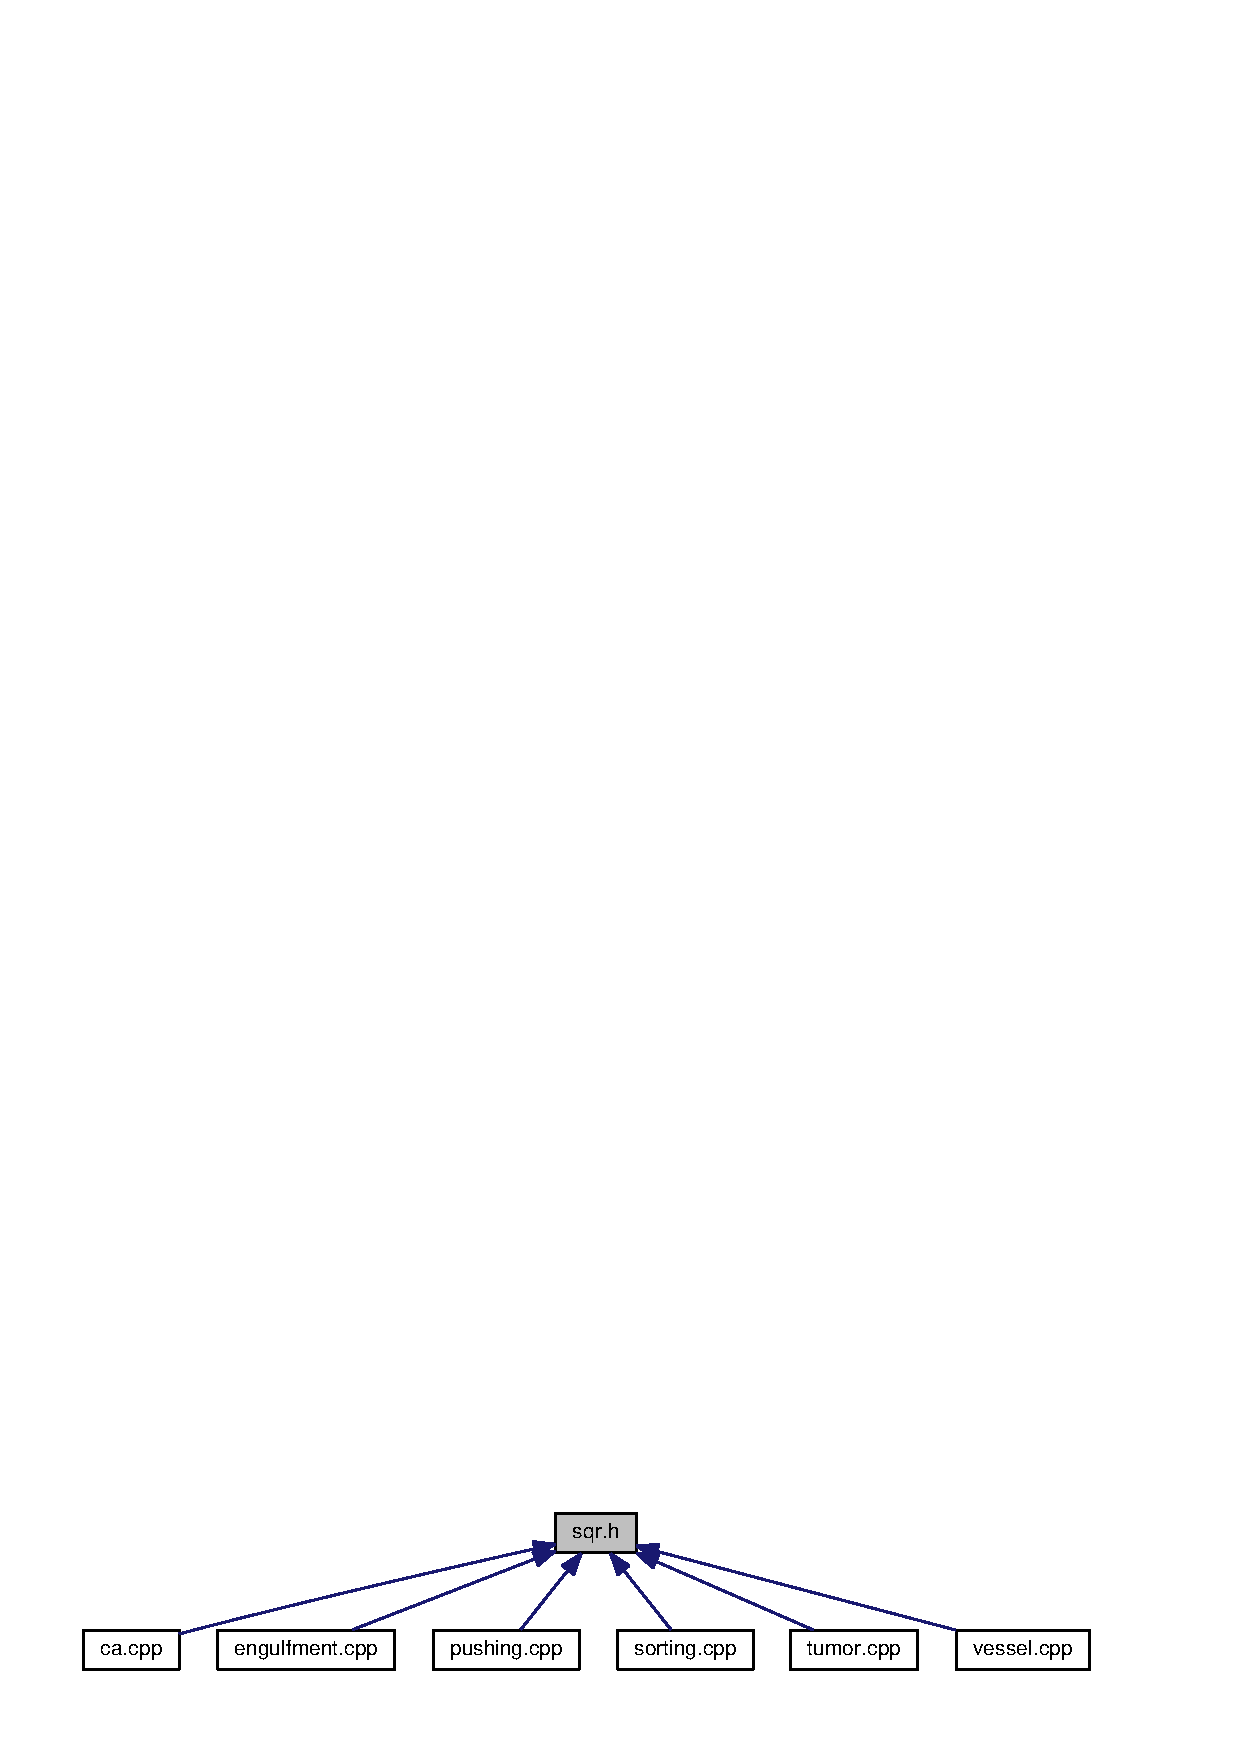
\includegraphics[width=350pt]{sqr_8h__dep__incl}
\end{center}
\end{figure}
\subsection*{Macros}
\begin{DoxyCompactItemize}
\item 
\#define {\bf S\-Q\-R}(a)~((sqrarg=(a)) == 0.\-0 ? 0.\-0 \-: sqrarg$\ast$sqrarg)
\item 
\#define {\bf D\-S\-Q\-R}(a)~((dsqrarg=(a)) == 0.\-0 ? 0.\-0 \-: dsqrarg$\ast$dsqrarg)
\end{DoxyCompactItemize}


\subsection{Macro Definition Documentation}
\index{sqr.\-h@{sqr.\-h}!D\-S\-Q\-R@{D\-S\-Q\-R}}
\index{D\-S\-Q\-R@{D\-S\-Q\-R}!sqr.h@{sqr.\-h}}
\subsubsection[{D\-S\-Q\-R}]{\setlength{\rightskip}{0pt plus 5cm}\#define D\-S\-Q\-R(
\begin{DoxyParamCaption}
\item[{}]{a}
\end{DoxyParamCaption}
)~((dsqrarg=(a)) == 0.\-0 ? 0.\-0 \-: dsqrarg$\ast$dsqrarg)}\label{sqr_8h_aa3c80caa06171d7fad9ab72cb3c9cd5b}
\index{sqr.\-h@{sqr.\-h}!S\-Q\-R@{S\-Q\-R}}
\index{S\-Q\-R@{S\-Q\-R}!sqr.h@{sqr.\-h}}
\subsubsection[{S\-Q\-R}]{\setlength{\rightskip}{0pt plus 5cm}\#define S\-Q\-R(
\begin{DoxyParamCaption}
\item[{}]{a}
\end{DoxyParamCaption}
)~((sqrarg=(a)) == 0.\-0 ? 0.\-0 \-: sqrarg$\ast$sqrarg)}\label{sqr_8h_ad41630f833e920c1ffa34722f45a8e77}

\section{sticky.\-h File Reference}
\label{sticky_8h}\index{sticky.\-h@{sticky.\-h}}
This graph shows which files directly or indirectly include this file\-:
\nopagebreak
\begin{figure}[H]
\begin{center}
\leavevmode
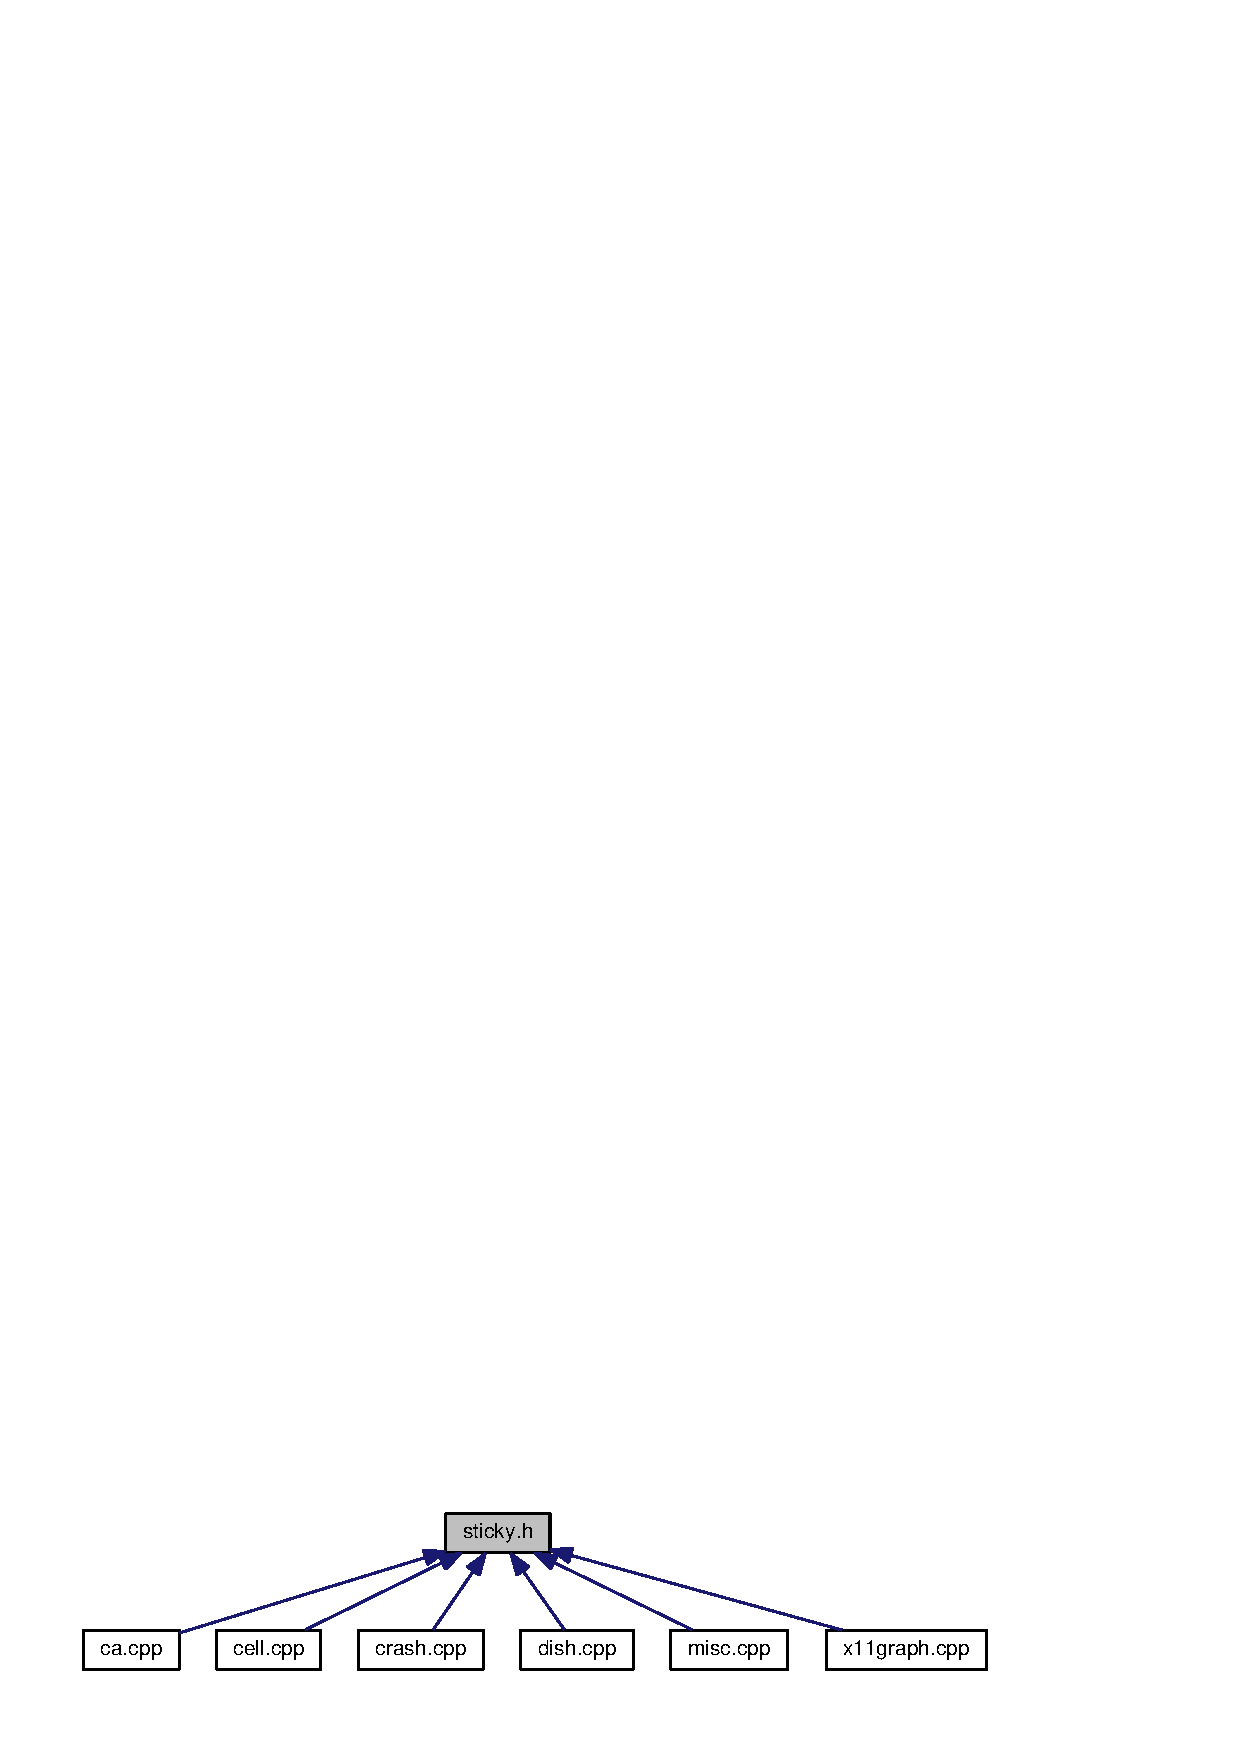
\includegraphics[width=350pt]{sticky_8h__dep__incl}
\end{center}
\end{figure}
\subsection*{Macros}
\begin{DoxyCompactItemize}
\item 
\#define {\bf G\-R\-I\-D\-X}~100
\item 
\#define {\bf G\-R\-I\-D\-Y}~100
\item 
\#define {\bf M\-A\-X\-C\-E\-L\-L\-S}~1024 /$\ast$  beware  $\ast$/
\item 
\#define {\bf M\-A\-X\-N\-E\-I\-G\-H}~2054
\item 
\#define {\bf F\-A\-L\-S\-E}~0
\item 
\#define {\bf T\-R\-U\-E}~1
\item 
\#define {\bf O\-K}~1
\item 
\#define {\bf T\-E\-S\-T\-C\-E\-L\-L\-S}~1
\item 
\#define {\bf B\-O\-L\-T\-Z\-M\-A\-N\-N}~1024
\item 
\#define {\bf M\-A\-X\-S\-E\-E\-D}~65531349
\item 
\#define {\bf M\-A\-X\-H\-I\-S\-T}~4096
\item 
\#define {\bf M\-A\-X\-T\-Y\-P\-E}~256
\item 
\#define {\bf W\-H\-I\-T\-E}~0
\item 
\#define {\bf B\-L\-A\-C\-K}~1
\item 
\#define {\bf R\-E\-D}~2
\item 
\#define {\bf B\-L\-U\-E}~3
\item 
\#define {\bf G\-R\-E\-E\-N}~4
\item 
\#define {\bf M\-E\-D\-I\-U\-M}~0
\item 
\#define {\bf E\-M\-P\-T\-Y}~-\/1
\item 
\#define {\bf D\-I\-V}~1   /$\ast$ D\-I\-V 2$^\wedge$(\# of divbit) $\ast$/
\item 
\#define {\bf R\-E\-M\-A\-R\-K}~56
\item 
\#define {\bf H\-A\-S\-H\-C\-O\-L\-P\-R\-I\-M\-E}~255
\item 
\#define {\bf P\-L\-O\-T\-P\-E\-R\-I\-O\-D\-F\-R\-E\-Q\-U\-E\-N\-C\-Y}~25
\item 
\#define {\bf H\-O\-S\-T\-D\-E\-A\-D}~-\/20
\item 
\#define {\bf N\-U\-L\-L\-\_\-\-B\-E\-A\-S\-T}~-\/10
\item 
\#define {\bf O\-K\-\_\-\-B\-E\-A\-S\-T}~-\/5
\item 
\#define {\bf P\-M\-U\-T}~0.\-009
\item 
\#define {\bf P\-M\-U\-T2}~.\-1
\item 
\#define {\bf D\-M\-U\-T}~0.\-0021
\item 
\#define {\bf P\-C\-O}~0.
\item 
\#define {\bf N\-E\-T\-S\-I\-Z\-E}~29
\item 
\#define {\bf I\-N\-E\-T\-S\-I\-Z\-E}~16
\item 
\#define {\bf I\-N\-P\-\_\-\-P\-R\-O\-T}~16 /$\ast$ number of negative inputs (connectivity) $\ast$/
\item 
\#define {\bf P\-O\-T\-P\-R\-O\-T}~16 /$\ast$ number of potential proteins $\ast$/
\item 
\#define {\bf C\-O\-M\-M\-U\-N\-I\-C\-A\-T\-I\-O\-N}~2
\item 
\#define {\bf E\-N\-E\-R\-G\-Y\-O\-F\-F\-S\-E\-T}~8
\item 
\#define {\bf N\-H\-H\-I\-S\-T}~10
\item 
\#define {\bf N\-H\-\_\-\-T\-H}~0.\-5
\item 
\#define {\bf E\-N\-D\-O\-F\-S\-T\-A\-T\-E\-S}~1$<$$<$({\bf N\-E\-T\-S\-I\-Z\-E}+2)
\end{DoxyCompactItemize}
\subsection*{Functions}
\begin{DoxyCompactItemize}
\item 
double {\bf R\-A\-N\-D\-O\-M} ()
\end{DoxyCompactItemize}


\subsection{Macro Definition Documentation}
\index{sticky.\-h@{sticky.\-h}!B\-L\-A\-C\-K@{B\-L\-A\-C\-K}}
\index{B\-L\-A\-C\-K@{B\-L\-A\-C\-K}!sticky.h@{sticky.\-h}}
\subsubsection[{B\-L\-A\-C\-K}]{\setlength{\rightskip}{0pt plus 5cm}\#define B\-L\-A\-C\-K~1}\label{sticky_8h_a7b3b25cba33b07c303f3060fe41887f6}
\index{sticky.\-h@{sticky.\-h}!B\-L\-U\-E@{B\-L\-U\-E}}
\index{B\-L\-U\-E@{B\-L\-U\-E}!sticky.h@{sticky.\-h}}
\subsubsection[{B\-L\-U\-E}]{\setlength{\rightskip}{0pt plus 5cm}\#define B\-L\-U\-E~3}\label{sticky_8h_a79d10e672abb49ad63eeaa8aaef57c38}
\index{sticky.\-h@{sticky.\-h}!B\-O\-L\-T\-Z\-M\-A\-N\-N@{B\-O\-L\-T\-Z\-M\-A\-N\-N}}
\index{B\-O\-L\-T\-Z\-M\-A\-N\-N@{B\-O\-L\-T\-Z\-M\-A\-N\-N}!sticky.h@{sticky.\-h}}
\subsubsection[{B\-O\-L\-T\-Z\-M\-A\-N\-N}]{\setlength{\rightskip}{0pt plus 5cm}\#define B\-O\-L\-T\-Z\-M\-A\-N\-N~1024}\label{sticky_8h_aa1487dae81baa2e0a5643e7b571633a0}
\index{sticky.\-h@{sticky.\-h}!C\-O\-M\-M\-U\-N\-I\-C\-A\-T\-I\-O\-N@{C\-O\-M\-M\-U\-N\-I\-C\-A\-T\-I\-O\-N}}
\index{C\-O\-M\-M\-U\-N\-I\-C\-A\-T\-I\-O\-N@{C\-O\-M\-M\-U\-N\-I\-C\-A\-T\-I\-O\-N}!sticky.h@{sticky.\-h}}
\subsubsection[{C\-O\-M\-M\-U\-N\-I\-C\-A\-T\-I\-O\-N}]{\setlength{\rightskip}{0pt plus 5cm}\#define C\-O\-M\-M\-U\-N\-I\-C\-A\-T\-I\-O\-N~2}\label{sticky_8h_ab45c9753cd336b5f0cb5d278b5547562}
\index{sticky.\-h@{sticky.\-h}!D\-I\-V@{D\-I\-V}}
\index{D\-I\-V@{D\-I\-V}!sticky.h@{sticky.\-h}}
\subsubsection[{D\-I\-V}]{\setlength{\rightskip}{0pt plus 5cm}\#define D\-I\-V~1   /$\ast$ D\-I\-V 2$^\wedge$(\# of divbit) $\ast$/}\label{sticky_8h_a8295e0aed07a8923d8363ce46c7b08e2}
\index{sticky.\-h@{sticky.\-h}!D\-M\-U\-T@{D\-M\-U\-T}}
\index{D\-M\-U\-T@{D\-M\-U\-T}!sticky.h@{sticky.\-h}}
\subsubsection[{D\-M\-U\-T}]{\setlength{\rightskip}{0pt plus 5cm}\#define D\-M\-U\-T~0.\-0021}\label{sticky_8h_a589694e83256d29f3f17d77aa5ee1468}
\index{sticky.\-h@{sticky.\-h}!E\-M\-P\-T\-Y@{E\-M\-P\-T\-Y}}
\index{E\-M\-P\-T\-Y@{E\-M\-P\-T\-Y}!sticky.h@{sticky.\-h}}
\subsubsection[{E\-M\-P\-T\-Y}]{\setlength{\rightskip}{0pt plus 5cm}\#define E\-M\-P\-T\-Y~-\/1}\label{sticky_8h_a2b7cf2a3641be7b89138615764d60ba3}


Referenced by Cell\-::\-Clear\-J(), and Cellular\-Potts\-::\-Search\-Nand\-Plot().

\index{sticky.\-h@{sticky.\-h}!E\-N\-D\-O\-F\-S\-T\-A\-T\-E\-S@{E\-N\-D\-O\-F\-S\-T\-A\-T\-E\-S}}
\index{E\-N\-D\-O\-F\-S\-T\-A\-T\-E\-S@{E\-N\-D\-O\-F\-S\-T\-A\-T\-E\-S}!sticky.h@{sticky.\-h}}
\subsubsection[{E\-N\-D\-O\-F\-S\-T\-A\-T\-E\-S}]{\setlength{\rightskip}{0pt plus 5cm}\#define E\-N\-D\-O\-F\-S\-T\-A\-T\-E\-S~1$<$$<$({\bf N\-E\-T\-S\-I\-Z\-E}+2)}\label{sticky_8h_a033f79766aaf51515318d900472434c2}
\index{sticky.\-h@{sticky.\-h}!E\-N\-E\-R\-G\-Y\-O\-F\-F\-S\-E\-T@{E\-N\-E\-R\-G\-Y\-O\-F\-F\-S\-E\-T}}
\index{E\-N\-E\-R\-G\-Y\-O\-F\-F\-S\-E\-T@{E\-N\-E\-R\-G\-Y\-O\-F\-F\-S\-E\-T}!sticky.h@{sticky.\-h}}
\subsubsection[{E\-N\-E\-R\-G\-Y\-O\-F\-F\-S\-E\-T}]{\setlength{\rightskip}{0pt plus 5cm}\#define E\-N\-E\-R\-G\-Y\-O\-F\-F\-S\-E\-T~8}\label{sticky_8h_a4d27595b7aa889871960faee4f07be06}
\index{sticky.\-h@{sticky.\-h}!F\-A\-L\-S\-E@{F\-A\-L\-S\-E}}
\index{F\-A\-L\-S\-E@{F\-A\-L\-S\-E}!sticky.h@{sticky.\-h}}
\subsubsection[{F\-A\-L\-S\-E}]{\setlength{\rightskip}{0pt plus 5cm}\#define F\-A\-L\-S\-E~0}\label{sticky_8h_aa93f0eb578d23995850d61f7d61c55c1}
\index{sticky.\-h@{sticky.\-h}!G\-R\-E\-E\-N@{G\-R\-E\-E\-N}}
\index{G\-R\-E\-E\-N@{G\-R\-E\-E\-N}!sticky.h@{sticky.\-h}}
\subsubsection[{G\-R\-E\-E\-N}]{\setlength{\rightskip}{0pt plus 5cm}\#define G\-R\-E\-E\-N~4}\label{sticky_8h_acfbc006ea433ad708fdee3e82996e721}
\index{sticky.\-h@{sticky.\-h}!G\-R\-I\-D\-X@{G\-R\-I\-D\-X}}
\index{G\-R\-I\-D\-X@{G\-R\-I\-D\-X}!sticky.h@{sticky.\-h}}
\subsubsection[{G\-R\-I\-D\-X}]{\setlength{\rightskip}{0pt plus 5cm}\#define G\-R\-I\-D\-X~100}\label{sticky_8h_a3e873381dde6998ffa24155ca5bdc8db}
\index{sticky.\-h@{sticky.\-h}!G\-R\-I\-D\-Y@{G\-R\-I\-D\-Y}}
\index{G\-R\-I\-D\-Y@{G\-R\-I\-D\-Y}!sticky.h@{sticky.\-h}}
\subsubsection[{G\-R\-I\-D\-Y}]{\setlength{\rightskip}{0pt plus 5cm}\#define G\-R\-I\-D\-Y~100}\label{sticky_8h_a9e2c4c6919f2d65845459e082e408903}
\index{sticky.\-h@{sticky.\-h}!H\-A\-S\-H\-C\-O\-L\-P\-R\-I\-M\-E@{H\-A\-S\-H\-C\-O\-L\-P\-R\-I\-M\-E}}
\index{H\-A\-S\-H\-C\-O\-L\-P\-R\-I\-M\-E@{H\-A\-S\-H\-C\-O\-L\-P\-R\-I\-M\-E}!sticky.h@{sticky.\-h}}
\subsubsection[{H\-A\-S\-H\-C\-O\-L\-P\-R\-I\-M\-E}]{\setlength{\rightskip}{0pt plus 5cm}\#define H\-A\-S\-H\-C\-O\-L\-P\-R\-I\-M\-E~255}\label{sticky_8h_a722a6ac399fb2f267d981dbe03b9f19c}
\index{sticky.\-h@{sticky.\-h}!H\-O\-S\-T\-D\-E\-A\-D@{H\-O\-S\-T\-D\-E\-A\-D}}
\index{H\-O\-S\-T\-D\-E\-A\-D@{H\-O\-S\-T\-D\-E\-A\-D}!sticky.h@{sticky.\-h}}
\subsubsection[{H\-O\-S\-T\-D\-E\-A\-D}]{\setlength{\rightskip}{0pt plus 5cm}\#define H\-O\-S\-T\-D\-E\-A\-D~-\/20}\label{sticky_8h_affbffb2cda53ff0b083eb936fd6a63fc}
\index{sticky.\-h@{sticky.\-h}!I\-N\-E\-T\-S\-I\-Z\-E@{I\-N\-E\-T\-S\-I\-Z\-E}}
\index{I\-N\-E\-T\-S\-I\-Z\-E@{I\-N\-E\-T\-S\-I\-Z\-E}!sticky.h@{sticky.\-h}}
\subsubsection[{I\-N\-E\-T\-S\-I\-Z\-E}]{\setlength{\rightskip}{0pt plus 5cm}\#define I\-N\-E\-T\-S\-I\-Z\-E~16}\label{sticky_8h_adaa6d88422473ffa47ccb883655b6805}
\index{sticky.\-h@{sticky.\-h}!I\-N\-P\-\_\-\-P\-R\-O\-T@{I\-N\-P\-\_\-\-P\-R\-O\-T}}
\index{I\-N\-P\-\_\-\-P\-R\-O\-T@{I\-N\-P\-\_\-\-P\-R\-O\-T}!sticky.h@{sticky.\-h}}
\subsubsection[{I\-N\-P\-\_\-\-P\-R\-O\-T}]{\setlength{\rightskip}{0pt plus 5cm}\#define I\-N\-P\-\_\-\-P\-R\-O\-T~16 /$\ast$ number of negative inputs (connectivity) $\ast$/}\label{sticky_8h_a37e8ab1e4485febfad36a87cf7c02e46}
\index{sticky.\-h@{sticky.\-h}!M\-A\-X\-C\-E\-L\-L\-S@{M\-A\-X\-C\-E\-L\-L\-S}}
\index{M\-A\-X\-C\-E\-L\-L\-S@{M\-A\-X\-C\-E\-L\-L\-S}!sticky.h@{sticky.\-h}}
\subsubsection[{M\-A\-X\-C\-E\-L\-L\-S}]{\setlength{\rightskip}{0pt plus 5cm}\#define M\-A\-X\-C\-E\-L\-L\-S~1024 /$\ast$  beware  $\ast$/}\label{sticky_8h_aebdcd55375f6299449092ca0c4695243}
\index{sticky.\-h@{sticky.\-h}!M\-A\-X\-H\-I\-S\-T@{M\-A\-X\-H\-I\-S\-T}}
\index{M\-A\-X\-H\-I\-S\-T@{M\-A\-X\-H\-I\-S\-T}!sticky.h@{sticky.\-h}}
\subsubsection[{M\-A\-X\-H\-I\-S\-T}]{\setlength{\rightskip}{0pt plus 5cm}\#define M\-A\-X\-H\-I\-S\-T~4096}\label{sticky_8h_a41ba038635d6b8c9533fdfc5e2cf55d6}
\index{sticky.\-h@{sticky.\-h}!M\-A\-X\-N\-E\-I\-G\-H@{M\-A\-X\-N\-E\-I\-G\-H}}
\index{M\-A\-X\-N\-E\-I\-G\-H@{M\-A\-X\-N\-E\-I\-G\-H}!sticky.h@{sticky.\-h}}
\subsubsection[{M\-A\-X\-N\-E\-I\-G\-H}]{\setlength{\rightskip}{0pt plus 5cm}\#define M\-A\-X\-N\-E\-I\-G\-H~2054}\label{sticky_8h_a2b7287bc638f867d58fe5d48703fbb03}
\index{sticky.\-h@{sticky.\-h}!M\-A\-X\-S\-E\-E\-D@{M\-A\-X\-S\-E\-E\-D}}
\index{M\-A\-X\-S\-E\-E\-D@{M\-A\-X\-S\-E\-E\-D}!sticky.h@{sticky.\-h}}
\subsubsection[{M\-A\-X\-S\-E\-E\-D}]{\setlength{\rightskip}{0pt plus 5cm}\#define M\-A\-X\-S\-E\-E\-D~65531349}\label{sticky_8h_a137e5553fa04907d478f603885f01548}
\index{sticky.\-h@{sticky.\-h}!M\-A\-X\-T\-Y\-P\-E@{M\-A\-X\-T\-Y\-P\-E}}
\index{M\-A\-X\-T\-Y\-P\-E@{M\-A\-X\-T\-Y\-P\-E}!sticky.h@{sticky.\-h}}
\subsubsection[{M\-A\-X\-T\-Y\-P\-E}]{\setlength{\rightskip}{0pt plus 5cm}\#define M\-A\-X\-T\-Y\-P\-E~256}\label{sticky_8h_afa3b7bd558114ea80d4a13d732b53dde}
\index{sticky.\-h@{sticky.\-h}!M\-E\-D\-I\-U\-M@{M\-E\-D\-I\-U\-M}}
\index{M\-E\-D\-I\-U\-M@{M\-E\-D\-I\-U\-M}!sticky.h@{sticky.\-h}}
\subsubsection[{M\-E\-D\-I\-U\-M}]{\setlength{\rightskip}{0pt plus 5cm}\#define M\-E\-D\-I\-U\-M~0}\label{sticky_8h_a455b219d48b21108576f53129be38c32}
\index{sticky.\-h@{sticky.\-h}!N\-E\-T\-S\-I\-Z\-E@{N\-E\-T\-S\-I\-Z\-E}}
\index{N\-E\-T\-S\-I\-Z\-E@{N\-E\-T\-S\-I\-Z\-E}!sticky.h@{sticky.\-h}}
\subsubsection[{N\-E\-T\-S\-I\-Z\-E}]{\setlength{\rightskip}{0pt plus 5cm}\#define N\-E\-T\-S\-I\-Z\-E~29}\label{sticky_8h_a1a35ff780ff7a491a27e5f5398a39916}
\index{sticky.\-h@{sticky.\-h}!N\-H\-\_\-\-T\-H@{N\-H\-\_\-\-T\-H}}
\index{N\-H\-\_\-\-T\-H@{N\-H\-\_\-\-T\-H}!sticky.h@{sticky.\-h}}
\subsubsection[{N\-H\-\_\-\-T\-H}]{\setlength{\rightskip}{0pt plus 5cm}\#define N\-H\-\_\-\-T\-H~0.\-5}\label{sticky_8h_ac52a6e7a1de4af11e3b76bd9ee1898d2}
\index{sticky.\-h@{sticky.\-h}!N\-H\-H\-I\-S\-T@{N\-H\-H\-I\-S\-T}}
\index{N\-H\-H\-I\-S\-T@{N\-H\-H\-I\-S\-T}!sticky.h@{sticky.\-h}}
\subsubsection[{N\-H\-H\-I\-S\-T}]{\setlength{\rightskip}{0pt plus 5cm}\#define N\-H\-H\-I\-S\-T~10}\label{sticky_8h_aa70e07fe7bdad62c8b9cf0b91e21104f}
\index{sticky.\-h@{sticky.\-h}!N\-U\-L\-L\-\_\-\-B\-E\-A\-S\-T@{N\-U\-L\-L\-\_\-\-B\-E\-A\-S\-T}}
\index{N\-U\-L\-L\-\_\-\-B\-E\-A\-S\-T@{N\-U\-L\-L\-\_\-\-B\-E\-A\-S\-T}!sticky.h@{sticky.\-h}}
\subsubsection[{N\-U\-L\-L\-\_\-\-B\-E\-A\-S\-T}]{\setlength{\rightskip}{0pt plus 5cm}\#define N\-U\-L\-L\-\_\-\-B\-E\-A\-S\-T~-\/10}\label{sticky_8h_ae6a4e91343e3d4972a664d1a4be283f8}
\index{sticky.\-h@{sticky.\-h}!O\-K@{O\-K}}
\index{O\-K@{O\-K}!sticky.h@{sticky.\-h}}
\subsubsection[{O\-K}]{\setlength{\rightskip}{0pt plus 5cm}\#define O\-K~1}\label{sticky_8h_aba51915c87d64af47fb1cc59348961c9}
\index{sticky.\-h@{sticky.\-h}!O\-K\-\_\-\-B\-E\-A\-S\-T@{O\-K\-\_\-\-B\-E\-A\-S\-T}}
\index{O\-K\-\_\-\-B\-E\-A\-S\-T@{O\-K\-\_\-\-B\-E\-A\-S\-T}!sticky.h@{sticky.\-h}}
\subsubsection[{O\-K\-\_\-\-B\-E\-A\-S\-T}]{\setlength{\rightskip}{0pt plus 5cm}\#define O\-K\-\_\-\-B\-E\-A\-S\-T~-\/5}\label{sticky_8h_ac8bdd93ad3cd3be1e1d3d8afad542497}
\index{sticky.\-h@{sticky.\-h}!P\-C\-O@{P\-C\-O}}
\index{P\-C\-O@{P\-C\-O}!sticky.h@{sticky.\-h}}
\subsubsection[{P\-C\-O}]{\setlength{\rightskip}{0pt plus 5cm}\#define P\-C\-O~0.}\label{sticky_8h_a7a089b66e242231a852fb911ea4ca636}
\index{sticky.\-h@{sticky.\-h}!P\-L\-O\-T\-P\-E\-R\-I\-O\-D\-F\-R\-E\-Q\-U\-E\-N\-C\-Y@{P\-L\-O\-T\-P\-E\-R\-I\-O\-D\-F\-R\-E\-Q\-U\-E\-N\-C\-Y}}
\index{P\-L\-O\-T\-P\-E\-R\-I\-O\-D\-F\-R\-E\-Q\-U\-E\-N\-C\-Y@{P\-L\-O\-T\-P\-E\-R\-I\-O\-D\-F\-R\-E\-Q\-U\-E\-N\-C\-Y}!sticky.h@{sticky.\-h}}
\subsubsection[{P\-L\-O\-T\-P\-E\-R\-I\-O\-D\-F\-R\-E\-Q\-U\-E\-N\-C\-Y}]{\setlength{\rightskip}{0pt plus 5cm}\#define P\-L\-O\-T\-P\-E\-R\-I\-O\-D\-F\-R\-E\-Q\-U\-E\-N\-C\-Y~25}\label{sticky_8h_ab378a69d1d734ac99bf650f87e407e07}
\index{sticky.\-h@{sticky.\-h}!P\-M\-U\-T@{P\-M\-U\-T}}
\index{P\-M\-U\-T@{P\-M\-U\-T}!sticky.h@{sticky.\-h}}
\subsubsection[{P\-M\-U\-T}]{\setlength{\rightskip}{0pt plus 5cm}\#define P\-M\-U\-T~0.\-009}\label{sticky_8h_af7a24d0d49a3310aea7c7eabb4834a5e}
\index{sticky.\-h@{sticky.\-h}!P\-M\-U\-T2@{P\-M\-U\-T2}}
\index{P\-M\-U\-T2@{P\-M\-U\-T2}!sticky.h@{sticky.\-h}}
\subsubsection[{P\-M\-U\-T2}]{\setlength{\rightskip}{0pt plus 5cm}\#define P\-M\-U\-T2~.\-1}\label{sticky_8h_ad4e4ff849ff6e653cbb4beb30e65de80}
\index{sticky.\-h@{sticky.\-h}!P\-O\-T\-P\-R\-O\-T@{P\-O\-T\-P\-R\-O\-T}}
\index{P\-O\-T\-P\-R\-O\-T@{P\-O\-T\-P\-R\-O\-T}!sticky.h@{sticky.\-h}}
\subsubsection[{P\-O\-T\-P\-R\-O\-T}]{\setlength{\rightskip}{0pt plus 5cm}\#define P\-O\-T\-P\-R\-O\-T~16 /$\ast$ number of potential proteins $\ast$/}\label{sticky_8h_a1689f56af09ad8a248d4afe4d05e18a4}
\index{sticky.\-h@{sticky.\-h}!R\-E\-D@{R\-E\-D}}
\index{R\-E\-D@{R\-E\-D}!sticky.h@{sticky.\-h}}
\subsubsection[{R\-E\-D}]{\setlength{\rightskip}{0pt plus 5cm}\#define R\-E\-D~2}\label{sticky_8h_a8d23feea868a983c8c2b661e1e16972f}
\index{sticky.\-h@{sticky.\-h}!R\-E\-M\-A\-R\-K@{R\-E\-M\-A\-R\-K}}
\index{R\-E\-M\-A\-R\-K@{R\-E\-M\-A\-R\-K}!sticky.h@{sticky.\-h}}
\subsubsection[{R\-E\-M\-A\-R\-K}]{\setlength{\rightskip}{0pt plus 5cm}\#define R\-E\-M\-A\-R\-K~56}\label{sticky_8h_ace9fba7267bf6a9a92654ce7f25c5516}
\index{sticky.\-h@{sticky.\-h}!T\-E\-S\-T\-C\-E\-L\-L\-S@{T\-E\-S\-T\-C\-E\-L\-L\-S}}
\index{T\-E\-S\-T\-C\-E\-L\-L\-S@{T\-E\-S\-T\-C\-E\-L\-L\-S}!sticky.h@{sticky.\-h}}
\subsubsection[{T\-E\-S\-T\-C\-E\-L\-L\-S}]{\setlength{\rightskip}{0pt plus 5cm}\#define T\-E\-S\-T\-C\-E\-L\-L\-S~1}\label{sticky_8h_aca55abd7a8e8b4195a0323a1a6a2e79c}
\index{sticky.\-h@{sticky.\-h}!T\-R\-U\-E@{T\-R\-U\-E}}
\index{T\-R\-U\-E@{T\-R\-U\-E}!sticky.h@{sticky.\-h}}
\subsubsection[{T\-R\-U\-E}]{\setlength{\rightskip}{0pt plus 5cm}\#define T\-R\-U\-E~1}\label{sticky_8h_aa8cecfc5c5c054d2875c03e77b7be15d}
\index{sticky.\-h@{sticky.\-h}!W\-H\-I\-T\-E@{W\-H\-I\-T\-E}}
\index{W\-H\-I\-T\-E@{W\-H\-I\-T\-E}!sticky.h@{sticky.\-h}}
\subsubsection[{W\-H\-I\-T\-E}]{\setlength{\rightskip}{0pt plus 5cm}\#define W\-H\-I\-T\-E~0}\label{sticky_8h_a87b537f5fa5c109d3c05c13d6b18f382}


\subsection{Function Documentation}
\index{sticky.\-h@{sticky.\-h}!R\-A\-N\-D\-O\-M@{R\-A\-N\-D\-O\-M}}
\index{R\-A\-N\-D\-O\-M@{R\-A\-N\-D\-O\-M}!sticky.h@{sticky.\-h}}
\subsubsection[{R\-A\-N\-D\-O\-M}]{\setlength{\rightskip}{0pt plus 5cm}double R\-A\-N\-D\-O\-M (
\begin{DoxyParamCaption}
\item[{void}]{}
\end{DoxyParamCaption}
)}\label{sticky_8h_af26e98955ff2eaaa6f4ee6b09ca07342}
\begin{DoxyReturn}{Returns}
A random double between 0 and 1 
\end{DoxyReturn}


References F\-A\-C, M\-B\-I\-G, M\-S\-E\-E\-D, and M\-Z.



Referenced by Cellular\-Potts\-::\-Amoebae\-Move(), Cellular\-Potts\-::\-Grow\-In\-Cells(), Random\-Number(), and Seed().


\section{tumor.\-cpp File Reference}
\label{tumor_8cpp}\index{tumor.\-cpp@{tumor.\-cpp}}
{\ttfamily \#include $<$stdio.\-h$>$}\\*
{\ttfamily \#include $<$malloc.\-h$>$}\\*
{\ttfamily \#include $<$iostream$>$}\\*
{\ttfamily \#include $<$cstdlib$>$}\\*
{\ttfamily \#include $<$algorithm$>$}\\*
{\ttfamily \#include $<$fstream$>$}\\*
{\ttfamily \#include $<$math.\-h$>$}\\*
{\ttfamily \#include \char`\"{}dish.\-h\char`\"{}}\\*
{\ttfamily \#include \char`\"{}random.\-h\char`\"{}}\\*
{\ttfamily \#include \char`\"{}cell.\-h\char`\"{}}\\*
{\ttfamily \#include \char`\"{}info.\-h\char`\"{}}\\*
{\ttfamily \#include \char`\"{}parameter.\-h\char`\"{}}\\*
{\ttfamily \#include \char`\"{}sqr.\-h\char`\"{}}\\*
{\ttfamily \#include \char`\"{}x11graph.\-h\char`\"{}}\\*
Include dependency graph for tumor.\-cpp\-:
\nopagebreak
\begin{figure}[H]
\begin{center}
\leavevmode
\includegraphics[width=350pt]{tumor_8cpp__incl}
\end{center}
\end{figure}

\section{vessel.\-cpp File Reference}
\label{vessel_8cpp}\index{vessel.\-cpp@{vessel.\-cpp}}
{\ttfamily \#include $<$stdio.\-h$>$}\\*
{\ttfamily \#include $<$malloc.\-h$>$}\\*
{\ttfamily \#include $<$iostream$>$}\\*
{\ttfamily \#include $<$cstdlib$>$}\\*
{\ttfamily \#include $<$algorithm$>$}\\*
{\ttfamily \#include $<$fstream$>$}\\*
{\ttfamily \#include $<$math.\-h$>$}\\*
{\ttfamily \#include \char`\"{}dish.\-h\char`\"{}}\\*
{\ttfamily \#include \char`\"{}random.\-h\char`\"{}}\\*
{\ttfamily \#include \char`\"{}cell.\-h\char`\"{}}\\*
{\ttfamily \#include \char`\"{}info.\-h\char`\"{}}\\*
{\ttfamily \#include \char`\"{}parameter.\-h\char`\"{}}\\*
{\ttfamily \#include \char`\"{}sqr.\-h\char`\"{}}\\*
{\ttfamily \#include \char`\"{}x11graph.\-h\char`\"{}}\\*
Include dependency graph for vessel.\-cpp\-:
\nopagebreak
\begin{figure}[H]
\begin{center}
\leavevmode
\includegraphics[width=350pt]{vessel_8cpp__incl}
\end{center}
\end{figure}

\section{warning.\-cpp File Reference}
\label{warning_8cpp}\index{warning.\-cpp@{warning.\-cpp}}
{\ttfamily \#include $<$stdarg.\-h$>$}\\*
{\ttfamily \#include $<$stdio.\-h$>$}\\*
{\ttfamily \#include $<$stdlib.\-h$>$}\\*
{\ttfamily \#include \char`\"{}warning.\-h\char`\"{}}\\*
Include dependency graph for warning.\-cpp\-:
\nopagebreak
\begin{figure}[H]
\begin{center}
\leavevmode
\includegraphics[width=305pt]{warning_8cpp__incl}
\end{center}
\end{figure}
\subsection*{Functions}
\begin{DoxyCompactItemize}
\item 
void {\bf error} (char $\ast$fmt,...)
\item 
void {\bf warning} (char $\ast$fmt,...)
\end{DoxyCompactItemize}
\subsection*{Variables}
\begin{DoxyCompactItemize}
\item 
int {\bf Quiet} =0
\end{DoxyCompactItemize}


\subsection{Function Documentation}
\index{warning.\-cpp@{warning.\-cpp}!error@{error}}
\index{error@{error}!warning.cpp@{warning.\-cpp}}
\subsubsection[{error}]{\setlength{\rightskip}{0pt plus 5cm}void error (
\begin{DoxyParamCaption}
\item[{char $\ast$}]{fmt, }
\item[{}]{...}
\end{DoxyParamCaption}
)}\label{warning_8cpp_aa7733e30b2951f225e24dca1ed4632b2}


Referenced by bgetpar(), Check\-File(), dgetparlist(), Parse\-Par(), Read\-Line(), Search\-Token(), and Skip\-Token().

\index{warning.\-cpp@{warning.\-cpp}!warning@{warning}}
\index{warning@{warning}!warning.cpp@{warning.\-cpp}}
\subsubsection[{warning}]{\setlength{\rightskip}{0pt plus 5cm}void warning (
\begin{DoxyParamCaption}
\item[{char $\ast$}]{fmt, }
\item[{}]{...}
\end{DoxyParamCaption}
)}\label{warning_8cpp_a03a9b4d67e93976f0e28d3c1a26cd9ef}


References Quiet.



Referenced by bgetpar(), dgetparlist(), fgetpar(), igetpar(), Parse\-Par(), Search\-Token(), and sgetpar().



\subsection{Variable Documentation}
\index{warning.\-cpp@{warning.\-cpp}!Quiet@{Quiet}}
\index{Quiet@{Quiet}!warning.cpp@{warning.\-cpp}}
\subsubsection[{Quiet}]{\setlength{\rightskip}{0pt plus 5cm}int Quiet =0}\label{warning_8cpp_a4cbc70c34829a2ba413672310bb6d528}


Referenced by warning().


\section{warning.\-h File Reference}
\label{warning_8h}\index{warning.\-h@{warning.\-h}}
This graph shows which files directly or indirectly include this file\-:
\nopagebreak
\begin{figure}[H]
\begin{center}
\leavevmode
\includegraphics[width=273pt]{warning_8h__dep__incl}
\end{center}
\end{figure}
\subsection*{Macros}
\begin{DoxyCompactItemize}
\item 
\#define {\bf M\-E\-M\-O\-R\-Y\-C\-H\-E\-C\-K}(x)~if ((x)==N\-U\-L\-L) \{   fprintf(stderr, \char`\"{}Out of Memory {\bf error} in \char`\"{}\#x\char`\"{} \textbackslash{}n\char`\"{});  exit(0); \}
\item 
\#define {\bf U\-N\-I\-D\-E\-N\-T\-I\-F\-I\-E\-D}~2353996
\end{DoxyCompactItemize}
\subsection*{Functions}
\begin{DoxyCompactItemize}
\item 
void {\bf error} (char $\ast$,...)
\item 
void {\bf warning} (char $\ast$,...)
\end{DoxyCompactItemize}


\subsection{Macro Definition Documentation}
\index{warning.\-h@{warning.\-h}!M\-E\-M\-O\-R\-Y\-C\-H\-E\-C\-K@{M\-E\-M\-O\-R\-Y\-C\-H\-E\-C\-K}}
\index{M\-E\-M\-O\-R\-Y\-C\-H\-E\-C\-K@{M\-E\-M\-O\-R\-Y\-C\-H\-E\-C\-K}!warning.h@{warning.\-h}}
\subsubsection[{M\-E\-M\-O\-R\-Y\-C\-H\-E\-C\-K}]{\setlength{\rightskip}{0pt plus 5cm}\#define M\-E\-M\-O\-R\-Y\-C\-H\-E\-C\-K(
\begin{DoxyParamCaption}
\item[{}]{x}
\end{DoxyParamCaption}
)~if ((x)==N\-U\-L\-L) \{   fprintf(stderr, \char`\"{}Out of Memory {\bf error} in \char`\"{}\#x\char`\"{} \textbackslash{}n\char`\"{});  exit(0); \}}\label{warning_8h_a4deefb7a45a2708e7102aded4cf38774}


Referenced by Read\-Line().

\index{warning.\-h@{warning.\-h}!U\-N\-I\-D\-E\-N\-T\-I\-F\-I\-E\-D@{U\-N\-I\-D\-E\-N\-T\-I\-F\-I\-E\-D}}
\index{U\-N\-I\-D\-E\-N\-T\-I\-F\-I\-E\-D@{U\-N\-I\-D\-E\-N\-T\-I\-F\-I\-E\-D}!warning.h@{warning.\-h}}
\subsubsection[{U\-N\-I\-D\-E\-N\-T\-I\-F\-I\-E\-D}]{\setlength{\rightskip}{0pt plus 5cm}\#define U\-N\-I\-D\-E\-N\-T\-I\-F\-I\-E\-D~2353996}\label{warning_8h_a0aa27ea24eb609b1568658c698607a5e}


\subsection{Function Documentation}
\index{warning.\-h@{warning.\-h}!error@{error}}
\index{error@{error}!warning.h@{warning.\-h}}
\subsubsection[{error}]{\setlength{\rightskip}{0pt plus 5cm}void error (
\begin{DoxyParamCaption}
\item[{char $\ast$}]{, }
\item[{}]{...}
\end{DoxyParamCaption}
)}\label{warning_8h_afca6a211b1e0fa85666abbc43cd5fbbb}


Referenced by bgetpar(), Check\-File(), dgetparlist(), Parse\-Par(), Read\-Line(), Search\-Token(), and Skip\-Token().

\index{warning.\-h@{warning.\-h}!warning@{warning}}
\index{warning@{warning}!warning.h@{warning.\-h}}
\subsubsection[{warning}]{\setlength{\rightskip}{0pt plus 5cm}void warning (
\begin{DoxyParamCaption}
\item[{char $\ast$}]{, }
\item[{}]{...}
\end{DoxyParamCaption}
)}\label{warning_8h_aece81b89be4e80015bb9981b6862914b}


References Quiet.



Referenced by bgetpar(), dgetparlist(), fgetpar(), igetpar(), Parse\-Par(), Search\-Token(), and sgetpar().


\section{x11graph.\-cpp File Reference}
\label{x11graph_8cpp}\index{x11graph.\-cpp@{x11graph.\-cpp}}
{\ttfamily \#include $<$stdio.\-h$>$}\\*
{\ttfamily \#include $<$unistd.\-h$>$}\\*
{\ttfamily \#include $<$X11/\-Xlib.\-h$>$}\\*
{\ttfamily \#include $<$X11/\-Xutil.\-h$>$}\\*
{\ttfamily \#include $<$X11/keysym.\-h$>$}\\*
{\ttfamily \#include $<$X11/cursorfont.\-h$>$}\\*
{\ttfamily \#include $<$math.\-h$>$}\\*
{\ttfamily \#include $<$malloc.\-h$>$}\\*
{\ttfamily \#include $<$stdlib.\-h$>$}\\*
{\ttfamily \#include $<$sys/types.\-h$>$}\\*
{\ttfamily \#include $<$sys/stat.\-h$>$}\\*
{\ttfamily \#include $<$fcntl.\-h$>$}\\*
{\ttfamily \#include $<$cstring$>$}\\*
{\ttfamily \#include $<$errno.\-h$>$}\\*
{\ttfamily \#include $<$png.\-h$>$}\\*
{\ttfamily \#include \char`\"{}sticky.\-h\char`\"{}}\\*
{\ttfamily \#include \char`\"{}x11graph.\-h\char`\"{}}\\*
{\ttfamily \#include \char`\"{}parameter.\-h\char`\"{}}\\*
{\ttfamily \#include \char`\"{}output.\-h\char`\"{}}\\*
{\ttfamily \#include $<$iostream$>$}\\*
{\ttfamily \#include $<$string$>$}\\*
Include dependency graph for x11graph.\-cpp\-:
\nopagebreak
\begin{figure}[H]
\begin{center}
\leavevmode
\includegraphics[width=350pt]{x11graph_8cpp__incl}
\end{center}
\end{figure}
\subsection*{Macros}
\begin{DoxyCompactItemize}
\item 
\#define {\bf N\-O\-P\-V\-M}
\item 
\#define {\bf K\-E\-Y\-B\-U\-F\-S\-I\-Z\-E}~10
\item 
\#define {\bf S\-W\-A\-P}(a, b)~tmpswap = a; a = b; b = tmpswap;
\end{DoxyCompactItemize}
\subsection*{Variables}
\begin{DoxyCompactItemize}
\item 
{\bf Parameter} {\bf par}
\item 
int {\bf errno}
\end{DoxyCompactItemize}


\subsection{Macro Definition Documentation}
\index{x11graph.\-cpp@{x11graph.\-cpp}!K\-E\-Y\-B\-U\-F\-S\-I\-Z\-E@{K\-E\-Y\-B\-U\-F\-S\-I\-Z\-E}}
\index{K\-E\-Y\-B\-U\-F\-S\-I\-Z\-E@{K\-E\-Y\-B\-U\-F\-S\-I\-Z\-E}!x11graph.cpp@{x11graph.\-cpp}}
\subsubsection[{K\-E\-Y\-B\-U\-F\-S\-I\-Z\-E}]{\setlength{\rightskip}{0pt plus 5cm}\#define K\-E\-Y\-B\-U\-F\-S\-I\-Z\-E~10}\label{x11graph_8cpp_a5058042f8d2b0be49f10f8c46b19a46a}


Referenced by X11\-Graphics\-::\-Get\-X\-Y\-Coo().

\index{x11graph.\-cpp@{x11graph.\-cpp}!N\-O\-P\-V\-M@{N\-O\-P\-V\-M}}
\index{N\-O\-P\-V\-M@{N\-O\-P\-V\-M}!x11graph.cpp@{x11graph.\-cpp}}
\subsubsection[{N\-O\-P\-V\-M}]{\setlength{\rightskip}{0pt plus 5cm}\#define N\-O\-P\-V\-M}\label{x11graph_8cpp_affeb851a50e0fe35fa29a8b04113bcf1}
\index{x11graph.\-cpp@{x11graph.\-cpp}!S\-W\-A\-P@{S\-W\-A\-P}}
\index{S\-W\-A\-P@{S\-W\-A\-P}!x11graph.cpp@{x11graph.\-cpp}}
\subsubsection[{S\-W\-A\-P}]{\setlength{\rightskip}{0pt plus 5cm}\#define S\-W\-A\-P(
\begin{DoxyParamCaption}
\item[{}]{a, }
\item[{}]{b}
\end{DoxyParamCaption}
)~tmpswap = a; a = b; b = tmpswap;}\label{x11graph_8cpp_aac9153aee4bdb92701df902e06a74eb3}


Referenced by X11\-Graphics\-::\-Line().



\subsection{Variable Documentation}
\index{x11graph.\-cpp@{x11graph.\-cpp}!errno@{errno}}
\index{errno@{errno}!x11graph.cpp@{x11graph.\-cpp}}
\subsubsection[{errno}]{\setlength{\rightskip}{0pt plus 5cm}int errno}\label{x11graph_8cpp_ad65a8842cc674e3ddf69355898c0ecbf}


Referenced by Check\-File(), Read\-Line(), and Search\-Token().

\index{x11graph.\-cpp@{x11graph.\-cpp}!par@{par}}
\index{par@{par}!x11graph.cpp@{x11graph.\-cpp}}
\subsubsection[{par}]{\setlength{\rightskip}{0pt plus 5cm}{\bf Parameter} par}\label{x11graph_8cpp_aa11a52593a908c20a7259a3e72c0b348}

\section{x11graph.\-h File Reference}
\label{x11graph_8h}\index{x11graph.\-h@{x11graph.\-h}}
{\ttfamily \#include $<$X11/\-Xlib.\-h$>$}\\*
{\ttfamily \#include $<$X11/\-Xutil.\-h$>$}\\*
{\ttfamily \#include $<$X11/keysym.\-h$>$}\\*
{\ttfamily \#include $<$X11/cursorfont.\-h$>$}\\*
{\ttfamily \#include \char`\"{}graph.\-h\char`\"{}}\\*
Include dependency graph for x11graph.\-h\-:
\nopagebreak
\begin{figure}[H]
\begin{center}
\leavevmode
\includegraphics[width=350pt]{x11graph_8h__incl}
\end{center}
\end{figure}
This graph shows which files directly or indirectly include this file\-:
\nopagebreak
\begin{figure}[H]
\begin{center}
\leavevmode
\includegraphics[width=350pt]{x11graph_8h__dep__incl}
\end{center}
\end{figure}
\subsection*{Classes}
\begin{DoxyCompactItemize}
\item 
struct {\bf li}
\item 
struct {\bf co}
\item 
class {\bf X11\-Graphics}
\begin{DoxyCompactList}\small\item\em X-\/\-Windows implementation of \doxyref{Graphics}{p.}{classGraphics} interface. \end{DoxyCompactList}\end{DoxyCompactItemize}
\subsection*{Macros}
\begin{DoxyCompactItemize}
\item 
\#define {\bf O\-U\-T\-F\-I\-L\-E}~\char`\"{}beestje.\-mov\char`\"{}
\item 
\#define {\bf C\-F\-I\-L\-E}~\char`\"{}sticky.\-ctb\char`\"{}
\item 
\#define {\bf V\-E\-R\-B\-O\-S\-E}~1
\item 
\#define {\bf R\-E\-S\-I\-Z\-E}~-\/20
\item 
\#define {\bf M\-O\-T\-I\-O\-N}~-\/21
\item 
\#define {\bf T\-I\-M\-E\-S\-T\-E\-P}~void {\bf X11\-Graphics\-::\-Time\-Step}(void)
\end{DoxyCompactItemize}
\subsection*{Typedefs}
\begin{DoxyCompactItemize}
\item 
typedef struct {\bf li} {\bf Line\-Type}
\item 
typedef struct {\bf co} {\bf Coordinate}
\end{DoxyCompactItemize}


\subsection{Macro Definition Documentation}
\index{x11graph.\-h@{x11graph.\-h}!C\-F\-I\-L\-E@{C\-F\-I\-L\-E}}
\index{C\-F\-I\-L\-E@{C\-F\-I\-L\-E}!x11graph.h@{x11graph.\-h}}
\subsubsection[{C\-F\-I\-L\-E}]{\setlength{\rightskip}{0pt plus 5cm}\#define C\-F\-I\-L\-E~\char`\"{}sticky.\-ctb\char`\"{}}\label{x11graph_8h_a3331b5c3a259278b37d3e1bdfccbc276}
\index{x11graph.\-h@{x11graph.\-h}!M\-O\-T\-I\-O\-N@{M\-O\-T\-I\-O\-N}}
\index{M\-O\-T\-I\-O\-N@{M\-O\-T\-I\-O\-N}!x11graph.h@{x11graph.\-h}}
\subsubsection[{M\-O\-T\-I\-O\-N}]{\setlength{\rightskip}{0pt plus 5cm}\#define M\-O\-T\-I\-O\-N~-\/21}\label{x11graph_8h_a37210bcb4e70d9199030fb7cd89135e7}


Referenced by X11\-Graphics\-::\-Get\-X\-Y\-Coo(), and X11\-Graphics\-::\-Replace\-Beast().

\index{x11graph.\-h@{x11graph.\-h}!O\-U\-T\-F\-I\-L\-E@{O\-U\-T\-F\-I\-L\-E}}
\index{O\-U\-T\-F\-I\-L\-E@{O\-U\-T\-F\-I\-L\-E}!x11graph.h@{x11graph.\-h}}
\subsubsection[{O\-U\-T\-F\-I\-L\-E}]{\setlength{\rightskip}{0pt plus 5cm}\#define O\-U\-T\-F\-I\-L\-E~\char`\"{}beestje.\-mov\char`\"{}}\label{x11graph_8h_a32cc9d976eaa3b33e3cdbc87e47c72a1}
\index{x11graph.\-h@{x11graph.\-h}!R\-E\-S\-I\-Z\-E@{R\-E\-S\-I\-Z\-E}}
\index{R\-E\-S\-I\-Z\-E@{R\-E\-S\-I\-Z\-E}!x11graph.h@{x11graph.\-h}}
\subsubsection[{R\-E\-S\-I\-Z\-E}]{\setlength{\rightskip}{0pt plus 5cm}\#define R\-E\-S\-I\-Z\-E~-\/20}\label{x11graph_8h_a9b5b3725cfd4e076e81c426cfb0ad4ff}


Referenced by X11\-Graphics\-::\-Get\-X\-Y\-Coo().

\index{x11graph.\-h@{x11graph.\-h}!T\-I\-M\-E\-S\-T\-E\-P@{T\-I\-M\-E\-S\-T\-E\-P}}
\index{T\-I\-M\-E\-S\-T\-E\-P@{T\-I\-M\-E\-S\-T\-E\-P}!x11graph.h@{x11graph.\-h}}
\subsubsection[{T\-I\-M\-E\-S\-T\-E\-P}]{\setlength{\rightskip}{0pt plus 5cm}\#define T\-I\-M\-E\-S\-T\-E\-P~void {\bf X11\-Graphics\-::\-Time\-Step}(void)}\label{x11graph_8h_a68ee019dafc12ee47d427cda7f17713e}
\index{x11graph.\-h@{x11graph.\-h}!V\-E\-R\-B\-O\-S\-E@{V\-E\-R\-B\-O\-S\-E}}
\index{V\-E\-R\-B\-O\-S\-E@{V\-E\-R\-B\-O\-S\-E}!x11graph.h@{x11graph.\-h}}
\subsubsection[{V\-E\-R\-B\-O\-S\-E}]{\setlength{\rightskip}{0pt plus 5cm}\#define V\-E\-R\-B\-O\-S\-E~1}\label{x11graph_8h_a42f8c497a1968074f38bf5055c650dca}


\subsection{Typedef Documentation}
\index{x11graph.\-h@{x11graph.\-h}!Coordinate@{Coordinate}}
\index{Coordinate@{Coordinate}!x11graph.h@{x11graph.\-h}}
\subsubsection[{Coordinate}]{\setlength{\rightskip}{0pt plus 5cm}typedef struct {\bf co}  {\bf Coordinate}}\label{x11graph_8h_a48265b73772f7edca92074dddc43139b}
\index{x11graph.\-h@{x11graph.\-h}!Line\-Type@{Line\-Type}}
\index{Line\-Type@{Line\-Type}!x11graph.h@{x11graph.\-h}}
\subsubsection[{Line\-Type}]{\setlength{\rightskip}{0pt plus 5cm}typedef struct {\bf li}  {\bf Line\-Type}}\label{x11graph_8h_ab775ac44b25dce4c719d40619cf5dd44}

%--- End generated contents ---

% Index
\newpage
\phantomsection
\addcontentsline{toc}{chapter}{Index}
\printindex

\end{document}
